\def\languageisfrench{}

\documentclass[a4paper,10pt]{article}

\usepackage[a4paper, top=2.5cm, bottom=2.2cm, left=2.2cm, right=2.2cm]{geometry} % Marge reduction.

\ifdefined\languageisfrench
	%% Language specific package
	\usepackage[french]{babel}
	\frenchbsetup{StandardLists=true} % Necessary to use enumitem with babel/french.
\fi

%% Font and typing packages
\usepackage{fontspec}
\setmainfont[
	Ligatures=TeX,
	SmallCapsFont={PT Serif}
	]{PT Serif} % default is Latin Modern
\newfontfamily\antiquefont[Ligatures=TeX]{Caslon Antique} % fancy font
\usepackage{microtype}			% Greatly improves general appearance of the text.
\usepackage{SIunits}			% Unit appearance.
\usepackage{ulem}				% To cross words out. Use \sout{}.

%% Array utilities
\usepackage{array}				% Additionnal options for arrays.
\usepackage{colortbl}			% Additionnal options for coloring arrays.
\usepackage[table]{xcolor}		% Auto alternate grey-white rows.
\usepackage[export]{adjustbox}		% Centered pics in tables
\usepackage{slashbox}		% diagonal slash in a cell

%% List utilities
\usepackage[inline]{enumitem}   % Display inline lists.
\usepackage{etoolbox}           % General utility. Good for lists for instance.
\usepackage{xparse}             % List utilities.

%% Frames
\usepackage{framed}				% Boxes.
\usepackage[framemethod=TikZ]{mdframed}% For fancy frames.
\usepackage{tikz}				% For fancy frames.
\usepackage{wrapfig}			% Fancy insertion of pics in text.

%% Page utilities
\usepackage{parskip} 			% no paragraph indentation and spaces between paragraphs.
\usepackage{multicol}			% Allows to divide a part of the page in multiple columns.
\usepackage{titlesec} 			% titles customization
\usepackage{caption}			% captions customization
\usepackage{fancyhdr}		% For custom headers and foot texts
\pagestyle{fancy}

%% TOC
\usepackage{tocloft} % http://ctan.org/pkg/tocloft
\usepackage[toc]{multitoc}
	
%% Others
\usepackage{xstring}            % String parsing, cutting, etc.
\usepackage[hidelinks, bookmarks=false, pdfdisplaydoctitle=true, pdfstartview=FitH, pdfpagelabels=false]{hyperref} % Links in PDF.

\makeatletter

%%% Language specific stuff

\ifdefined\languageisfrench
	
\newcommand{\translationteam}{\item \og AEnoriel \fg \item \og Anglachel \fg \item \og Astadriel \fg \item \og Batcat \fg \item \og Bigfish \fg \item \og Eru \fg  \item \og Gandarin \fg \item \og Groumbahk \fg \item \og Iluvatar \fg \item \og Mammstein \fg \item \og Shlagrabak \fg \item et beaucoup d'autres...}

\hypersetup{
	pdfauthor={Équipe de traduction française de T9A},
	pdfsubject={Règles pour le jeu Batailles Fantastiques : Le 9\ieme{} Âge},
}

%%% Commands %%%

\ifdef{\isitanAB}{

\newcommand{\addtosortedlist}[1]{%
	\protected@edef\textarg{#1}%
	\protected@edef\textwithoutspaces{\expandafter\removespaces\expandafter{\textarg}}%
	\substitute\textwithoutspaces{É}{E}% Most used special characters of the language, and equivalent for alphabetical ordering
	\substitute\textwithoutspaces{È}{E}%
	\substitute\textwithoutspaces{Ê}{E}%
	\substitute\textwithoutspaces{é}{e}%
	\substitute\textwithoutspaces{è}{e}%
	\substitute\textwithoutspaces{ê}{e}%
	\substitute\textwithoutspaces{À}{A}%
	\substitute\textwithoutspaces{à}{a}%
	\substitute\textwithoutspaces{ù}{u}%
	\expandafter\sortitem\expandafter[\textwithoutspaces]{#1}%
}%

\newcommand{\pts}[1]{% First step is to remove spaces if there are some
	\def\numberwithoutspaces{\expandafter\removespaces\expandafter{#1}}%
	% Next step is getting rid of formatting if there are any (bold, color, ...)
	\pdfstringdef\cleannumber{\numberwithoutspaces}%
	% Now we can try if it is 1 or not
	\expandafter\ifstrequal\expandafter{\cleannumber}{1}{#1~\labels@point}{%
	\expandafter\ifstrequal\expandafter{\cleannumber}{0.5}{0,5~\labels@point}{%
	\expandafter\ifstrequal\expandafter{\cleannumber}{1.5}{1,5~\labels@point}{%
	#1~\labels@points}}}%
}

}{}

% Dark gods
\newcommand{\dchange}{Changement}
\newcommand{\dlust}{Luxure}
\newcommand{\pestilence}{Pestilence}
\newcommand{\wrath}{Courroux}
\newcommand{\truechaos}{Chaos Primordial}


% Nothing to edit here

\ifdef{\isitanAB}{

\newcommand{\alliancepts}[1]{
\ifsubstring{#1}{\free}{%
		\free{}%
	}{%
	\ifsubstring{#1}{\permodel}{%
		\splitatinf{#1}\myoption\myvalue%
		\pts{\myvalue}\permodel{}%
	}{%
	\pts{#1}
	}}
}

% You might wanna change the order of the gods - advanced user
\newcommand{\allianceoptions}[1]{%
	\defallianceoptions{#1}%
	\unitentryformat{\labels@allianceoptions\spacebeforecolon{}:}\newline
	\expandafter\ifblank\expandafter{\allianceoptions@introsentence}{}{\noindent\allianceoptions@introsentence{}\spacebeforecolon{}:}
	
	\expandafter\ifblank\expandafter{\allianceoptions@wrath}{
		\setlength{\columnseprule}{0.5pt}
		\renewcommand{\columnseprulecolor}{\color{black!30}}
		\vspace*{-0.2cm}\begin{multicols}{3}\raggedcolumns
		
			\begin{center}
			\noindent\dchange{}
			
			\noindent\alliancepts{\allianceoptions@change}
			\vspace*{-0.3cm}
			\end{center}
		
		\columnbreak
		
			\begin{center}
			\noindent\dlust{}
			
			\noindent\alliancepts{\allianceoptions@lust}
			\vspace*{-0.3cm}
			\end{center}
		
		\columnbreak

			\begin{center}
			\noindent\pestilence{}
			
			\noindent\alliancepts{\allianceoptions@pestilence}
			\vspace*{-0.3cm}
			\end{center}
			
		\end{multicols}
		\setlength{\columnseprule}{0pt}	
	}{
		\setlength{\columnseprule}{0.5pt}
		\renewcommand{\columnseprulecolor}{\color{black!30}}
		\vspace*{-0.2cm}\begin{multicols}{4}\raggedcolumns
		
			\begin{center}
			\noindent\dchange{}
			
			\noindent\alliancepts{\allianceoptions@change}
			\vspace*{-0.3cm}
			\end{center}
		
		\columnbreak

			\begin{center}
			\noindent\wrath{}
			
			\noindent\alliancepts{\allianceoptions@wrath}
			\vspace*{-0.3cm}
			\end{center}
		
		\columnbreak
		
			\begin{center}
			\noindent\dlust{}
			
			\noindent\alliancepts{\allianceoptions@lust}
			\vspace*{-0.3cm}
			\end{center}
		
		\columnbreak

			\begin{center}
			\noindent\pestilence{}
			
			\noindent\alliancepts{\allianceoptions@pestilence}
			\vspace*{-0.3cm}
			\end{center}
			
		\end{multicols}
		\setlength{\columnseprule}{0pt}
	}
}

}{}


%%% Labels %%%

% Profile

\newcommand{\labels@M}{M}
\newcommand{\labels@WS}{CC}
\newcommand{\labels@BS}{CT}
\newcommand{\labels@S}{F}
\newcommand{\labels@T}{E}
\newcommand{\labels@W}{PV}
\newcommand{\labels@I}{I}
\newcommand{\labels@A}{A}
\newcommand{\labels@Ld}{Cd}
\newcommand{\labels@Invocation}{Invocation} % For Vampire Covenant profiles
\newcommand{\labels@roundbase}{rond} % printed after XX mm for round bases

\newcommand{\Strength}{Force}

% Technical

\newcommand{\labels@range}{Portée}
\newcommand{\labels@point}{pt}
\newcommand{\labels@points}{pts}
\newcommand{\labels@only}{uniquement}
\newcommand{\labels@magic}{Magie}
\newcommand{\labels@pathsused}{Génère ses sorts dans la Discipline}
\newcommand{\labels@model}{figurine}
\newcommand{\labels@models}{figurines}
\newcommand{\labels@Singlemodel}{Figurine \textbf{seule}}

% Unit entry labels

\newcommand{\labels@basesize}{Socle}
\newcommand{\labels@trooptype}{Type de troupe}
\newcommand{\labels@specialrules}{Règles Spéciales}
\newcommand{\labels@alignment}{Allégeance}
\newcommand{\labels@alliance}{Allégeance}
\newcommand{\labels@allianceoptions}{Options d'Allégeance}
\newcommand{\labels@greenhiderace}{Race de Peaux Vertes}
\newcommand{\labels@equipment}{Équipement}
\newcommand{\labels@weapons}{Armes}
\newcommand{\labels@armour}{Armure}
\newcommand{\labels@options}{Options}
\newcommand{\labels@commandgroup}{État-Major}
\newcommand{\labels@charactermounts}{Montures de Personnages}
\newcommand{\labels@mounts}{Montures}
\newcommand{\labels@mount}{Monture}
\newcommand{\labels@specialequipment}{Équipement Spécial}

% Command groups

\newcommand{\labels@champion}{Champion}
\newcommand{\labels@standardbearer}{Porte-Étendard}
\newcommand{\labels@musician}{Musicien}
\newcommand{\labels@singlebannerallowance}{Une seule unité de ce type peut prendre une Bannière Magique}
\newcommand{\labels@condsinglebannerallowance}{Une seule unité de ce type peut prendre une Bannière Magique si}
\newcommand{\labels@bannerallowance}{Bannière Magique}
\newcommand{\labels@veteranstandardbearer}{Peut devenir Porte-Étendard Vétéran}
\newcommand{\labels@championallowance}{Arme Magique}

% Titles

\newcommand{\labels@armylist}{Liste des Troupes}
\newcommand{\labels@lords}{Seigneurs}
\newcommand{\labels@heroes}{Héros}
\newcommand{\labels@coreunits}{Unités de Base}
\newcommand{\labels@specialunits}{Unités Spéciales}
\newcommand{\labels@rareunits}{Unités Rares}
\newcommand{\labels@armywiderules}{Règles Communes de l'Armée}
\newcommand{\labels@armyspecialrules}{Règles Spéciales de l'Armée}
\newcommand{\labels@armoury}{Armurerie}
\newcommand{\labels@magicalitems}{Objets Magiques}
\newcommand{\labels@magicalweapons}{Armes Magiques}
\newcommand{\labels@magicalarmour}{Armures Magiques}
\newcommand{\labels@talismans}{Talismans}
\newcommand{\labels@enchanteditems}{Objets Enchantés}
\newcommand{\labels@arcaneitems}{Objets Cabalistiques}
\newcommand{\labels@magicalbanners}{Bannières Magiques}
\newcommand{\labels@quickrefsheet}{Fiche de Référence}
\newcommand{\labels@changelog}{Change Log}

\newcommand{\labels@lordsInitial}{S}
\newcommand{\labels@heroesInitial}{H}
\newcommand{\labels@coreunitsInitial}{B}
\newcommand{\labels@specialunitsInitial}{S}
\newcommand{\labels@rareunitsInitial}{R}
\newcommand{\labels@mountsInitial}{M}


% Titlepage

\newcommand{\labels@fantasybattles}{Batailles Fantastiques}
\newcommand{\labels@NinthAge}{Le 9\ieme{} Âge}
\newcommand{\labels@armyrules}{Règles de l'Armée}
\newcommand{\labels@frontpagecredits}{%
\labels@fantasybattles{} : \labels@NinthAge{} est un jeu créé et entretenu par la communauté qui met en scène des affrontements de figurines.\newline
Toutes les règles sont disponibles gratuitement sur le site suivant. Vos retours et suggestions sont les bienvenus : \url{http://www.the-ninth-age.com/}
}
\newcommand{\labels@license}{Copyright Creative Commons license : \url{the-ninth-age.com/license.html}}
\newcommand{\labels@tableofcontents}{Sommaire}
\newcommand{\labels@introduction}{%
\begin{center}\noindent{\Largerfontsize\textbf{Note des traducteurs}}\end{center}
\vspace{0.5cm}

Nous souhaitons remercier chaleureusement l'équipe à l'initiative du 9\ieme{} Âge pour leur motivation et leur travail continu pour faire vivre notre passion. Nous espérons que ce jeu saura développer les qualités pour plaire au plus grand nombre et réunir les joueurs, amateurs comme habitués des tournois, autour de règles amusantes et équilibrées, pour finalement s'imposer comme un standard du jeu de figurines. Une grande ambition qui ne pourra s'accomplir que \textbf{grâce à vous}, la communauté, via des retours constructifs, afin de modeler le jeu selon nos désirs. N'étant \textbf{en aucun cas à but lucratif}, le 9\ieme{} Âge part avec un avantage considérable. Les règles des éventuelles nouvelles sorties ne sont pas dictées par le besoin de vendre ces nouveautés. Vous pouvez choisir et acheter vos figurines où bon vous semble, il n'y a pas un unique revendeur toléré. Enfin, vous pouvez être assurés que tant que le 9\ieme{} Âge sera joué, vous disposerez d'un \textbf{support continu et régulier}, celui-ci étant offert par la communauté.

Concernant la traduction en elle-même, nous avons fait de notre mieux pour vous offrir une version de qualité, dont nous espérons qu'elle surpasse celle de la version originale ! Si vous constatez des coquilles, des erreurs, merci de nous les signaler en nous contactant sur le forum du 9\ieme{} Âge, dans le \textbf{sous-forum français} (\url{http://www.the-ninth-age.com/index.php?board/117-french/}). Vous y trouverez aussi les dernières mises à jour. \textbf{En cas de conflit d'interprétation avec la version originale, la version originale fait référence}.

\vspace{0.5cm}
Que ce jeu vous apporte d'innombrables heures de plaisir partagé !

\vspace{1cm}

\ifdef{\translationteam}{
	\begin{multicols}{3}
	\begin{itemize}
		\translationteam
	\end{itemize}
	\end{multicols}
}{}
}
\newcommand{\labels@rulechanges}{% blank ATM
}
\newcommand{\labels@latexcredit}{Document réalisé à l'aide de \LaTeX .}


%%% Technical commands

\newcommand{\only}[1]{(#1 uniquement)}
\newcommand{\free}{gratuit}
\newcommand{\upto}{jusqu'à}
\newcommand{\Upto}{Jusqu'à}
\newcommand{\unlimited}{pas de limite}
\newcommand{\permodel}{/fig.}
\newcommand{\listlastchoice}{ ou}
\newcommand{\notif}[1]{(pas #1)}
\newcommand{\wordand}{et}
\newcommand{\wordwith}{avec}
\newcommand{\ifNmodelsorless}[1]{(#1 figurines ou moins)}
\newcommand{\unitwith}{unité avec}
\newcommand{\From}{De} % From ... to ... models
\newcommand{\wordto}{à}
\newcommand{\wordAll}{Tous}
\newcommand{\spacebeforecolon}{ } % French put a space before colons
\newcommand{\minprice}{Coût min. :}
\newcommand{\mincostfor}{Coût min. pour}
\newcommand{\maxunitsize}{Taille max.}
\newcommand{\additionalfigscost}{Les figurines additionnelles coûtent}


%%% Special rules %%%

\newcommand{\ambush}{Embuscade}
\newcommand{\armourpiercing}[1]{Perforant\ifblank{#1}{}{ (#1)}}
\newcommand{\bodyguard}[1]{Garde du Corps\ifblank{#1}{}{ (#1)}}
\newcommand{\breathweapon}[1]{Attaque de Souffle\ifblank{#1}{}{ (#1)}}
\newcommand{\channel}{Canalisation}
\newcommand{\crushattack}{Attaque Écrasante}
\newcommand{\daemonicinstability}{Instabilité Démoniaque}
\newcommand{\devastatingcharge}{Charge Dévastatrice}
\newcommand{\distracting}{Distrayant}
\newcommand{\divineattacks}{Attaques Divines}
\newcommand{\engineer}{Ingénieur}
\newcommand{\ethereal}{Éthéré}
\newcommand{\fastcavalry}{Cavalerie Légère}
\newcommand{\fear}{Peur}
\newcommand{\fightinextrarank}{Combat avec un Rang Supplémentaire}
\newcommand{\fireborn}{Né du Feu}
\newcommand{\flamingattacks}{Attaques Enflammées}
\newcommand{\flammable}{Inflammable}
\newcommand{\frenzy}{Frénésie}
\newcommand{\fly}[1]{Vol\ifblank{#1}{}{ (#1)}}
\newcommand{\grindingattacks}[1]{Attaques de Broyage\ifblank{#1}{}{ (#1)}}
\newcommand{\hardtarget}{Camouflé}
\newcommand{\hatred}{Haine}
\newcommand{\hellfire}{Feu Démoniaque}
\newcommand{\hidden}{Caché}
\newcommand{\holyattacks}{Attaques Divines} % deprecated, still has to be filled. same as Divine Attacks.
\newcommand{\immunetopsychology}{Immunisé à la Psychologie}
\newcommand{\impacthits}[1]{Touches d'Impact\ifblank{#1}{}{ (#1)}}
\newcommand{\insignificant}{Insignifiant}
\newcommand{\largetarget}{Grande Cible}
\newcommand{\lethalstrike}{Coup Fatal}
\newcommand{\lightningattacks}{Attaques Foudroyantes}
\newcommand{\lightningreflexes}{Réflexes Foudroyants}
\newcommand{\lighttroops}{Troupe Légère}
\newcommand{\magicresistance}[1]{Résistance à la Magie\ifblank{#1}{}{ (#1)}}
\newcommand{\magicalattacks}{Attaques Magiques}
\newcommand{\metalshifting}{Fusion du Métal}
\newcommand{\moveorfire}{Mouvement ou Tir}
\newcommand{\multipleshots}[1]{Tirs Multiples\ifblank{#1}{}{ (#1)}}
\newcommand{\multiplewounds}[2]{Blessures Multiples\ifblank{#1}{}{ (#1\ifblank{#2}{)}{, #2)}}}
\newcommand{\notaleader}{Pas un Meneur}
\newcommand{\otherworldly}{D'Outre-Monde}
\newcommand{\pathmaster}[1]{Maître de la Voie\ifblank{#1}{}{ (#1)}}
\newcommand{\poisonedattacks}{Attaques Empoisonnées}
\newcommand{\quicktofire}{Tir Rapide}
\newcommand{\randommovement}[1]{Mouvement Aléatoire\ifblank{#1}{}{ (#1)}}
\newcommand{\randomattacks}[1]{Attaques Aléatoires\ifblank{#1}{}{ (#1)}}
\newcommand{\regeneration}[1]{Régénération\ifblank{#1}{}{ (#1+)}}
\newcommand{\reload}{Rechargez !}
\newcommand{\requirestwohands}{Arme à deux Mains}
\newcommand{\scythes}{Faux}
\newcommand{\scout}{Éclaireur}
\newcommand{\scouts}{Éclaireurs}
\newcommand{\stomp}[1]{Piétinement\ifblank{#1}{}{ (#1)}}
\newcommand{\strider}[1]{Guide\ifblank{#1}{}{ (#1)}}
\newcommand{\stubborn}{Tenace}
\newcommand{\stupidity}{Stupidité}
\newcommand{\skirmisher}{Tirailleur}
\newcommand{\skirmishers}{Tirailleurs}
\newcommand{\sweepingattack}{Attaque au Passage}
\newcommand{\swiftstride}{Course Rapide}
\newcommand{\thunderouscharge}{Charge Tonitruante}
\newcommand{\terror}{Terreur}
\newcommand{\toxicattacks}{Attaques Toxiques}
\newcommand{\unbreakable}{Indémoralisable}
\newcommand{\undead}{Mort-Vivant}
\newcommand{\unstable}{Instable}
\newcommand{\unwieldy}{Encombrant}
\newcommand{\vanguard}{Avant-Garde}
\newcommand{\volleyfire}{Tir de Volée}
\newcommand{\warplatform}{Plateforme de Guerre}
\newcommand{\wardsave}[1]{Sauvegarde Invulnérable\ifblank{#1}{}{ (#1+)}}
\newcommand{\weaponmaster}{Maître d'Ar\-mes}
\newcommand{\wizardconclave}[1]{Conclave de Sorciers\ifblank{#1}{}{ (#1)}}


%%% Magic %%%


% General

\newcommand{\Pathof}{Voie}

\newcommand{\battle}{Commune}

\newcommand{\anyofthebattlemagic}{dans n'importe laquelle des Voies Communes}
\newcommand{\ONLYanyofthebattlemagic}{Commune de votre choix}

\newcommand{\magiclevel}[1]{\ifnumcomp{#1}{<}{3}{Apprenti Magicien}{Maître Magicien} Niveau #1}
\newcommand{\Level}{Niveau}

\newcommand{\wizard}{Magicien}
\newcommand{\wizards}{Magiciens}

\newcommand{\learnedspell}{Sort Appris}
\newcommand{\learnedspells}{Sorts Appris}
\newcommand{\attributespell}{Attribut de la Voie}
\newcommand{\attributespells}{Attributs de la Voie}
\newcommand{\attributespellnumber}{A}
\newcommand{\traitspell}{Sort Caractéristique}
\newcommand{\traitspells}{Sorts Caractéristiques}
\newcommand{\traitspellnumber}{C}


\newcommand{\boundspell}[1]{Objet de Sort\ifblank{#1}{}{, Puissance #1}}
\newcommand{\boundspells}[1]{Objets de Sort\ifblank{#1}{}{, Puissance #1}}

% Casting Vocabulary

\newcommand{\lostfocus}{Perte de Concentration}
\newcommand{\miscast}{Fiasco}
\newcommand{\miscasts}{Fiascos}
\newcommand{\overwhelmingpower}{Pouvoir Irrésistible}

\newcommand{\breachintheveil}{Brèche dans le Voile}
\newcommand{\catastrophicdetonation}{Explosion Catastrophique}
\newcommand{\witchfire}{Feu de Sorcières}
\newcommand{\sorcerousbacklash}{Contrecoup Magique}
\newcommand{\amnesia}{Amnésie}

% Spell Types

\newcommand{\augment}{Amélioration}
\newcommand{\hex}{Malédiction}
\newcommand{\universal}{Universel}
\newcommand{\missile}{Projectile}
\newcommand{\damage}{Dégâts}
\newcommand{\direct}{Direct}
\newcommand{\focused}{Focalisé}
\newcommand{\vortex}{Vortex}
\newcommand{\ground}{Marqueur}
\newcommand{\linetemplate}{Gabarit de Ligne}
\newcommand{\specialTYPE}{Spécial}
\newcommand{\aura}{Aura}
\newcommand{\castersunit}{Unité du Lanceur}
\newcommand{\caster}{Lanceur}

\newcommand{\template}{Gabarit}

% Spell Durations

\newcommand{\lastsoneturn}{Dure un Tour}
\newcommand{\instant}{Immédiat}
\newcommand{\permanent}{Permanent}
\newcommand{\remainsinplay}{Reste en Jeu}


% Battle Magic

\newcommand{\alchemy}{de l'Alchimie}
\newcommand{\alchemyattribute}{Édit de Fer}
\newcommand{\alchemysignature}{Métal Fondu}
\newcommand{\alchemyspellone}{Lames Enchantées}
\newcommand{\alchemyspelltwo}{Corrosion Rampante}
\newcommand{\alchemyspellthree}{Manteau de Vif-Argent}
\newcommand{\alchemyspellfour}{Pieu d'Argent}
\newcommand{\alchemyspellfive}{Fléau de l'Acier}
\newcommand{\alchemyspellsix}{Transmutation en Or}

\newcommand{\death}{de la Mort}
\newcommand{\deathattribute}{Nuage de Désespoir}
\newcommand{\deathsignature}{Le Baiser de la Faucheuse}
\newcommand{\deathspellone}{Malédiction du Mortel}
\newcommand{\deathspelltwo}{Esprits Dévorants}
\newcommand{\deathspellthree}{Sangsue Psychique}
\newcommand{\deathspellfour}{Moisson d’Âmes}
\newcommand{\deathspellfive}{L’Abîme aussi te Regarde...}
\newcommand{\deathspellsix}{Maelström d’Âmes}

\newcommand{\fire}{du Feu}
\newcommand{\fireattribute}{Feu Déchaîné}
\newcommand{\firesignature}{Boule de Feu}
\newcommand{\firespellone}{Cascade Ardente}
\newcommand{\firespelltwo}{Épées Flamboyantes}
\newcommand{\firespellthree}{Jet de Flammes}
\newcommand{\firespellfour}{Traits Enflammés}
\newcommand{\firespellfive}{Remparts Incandescents}
\newcommand{\firespellsix}{Souffler sur les Braises}

\newcommand{\heavens}{des Cieux}
\newcommand{\heavensattribute}{Second Sceau}
\newcommand{\heavenssignature}{Aquilon}
\newcommand{\heavensspellone}{Bourrasque}
\newcommand{\heavensspelltwo}{Choc Foudroyant}
\newcommand{\heavensspellthree}{Conjonction Astrale}
\newcommand{\heavensspellfour}{Fléau du Ponant}
\newcommand{\heavensspellfive}{Déluge d'Éclairs}
\newcommand{\heavensspellsix}{Appel de la Comète}

\newcommand{\light}{de la Lumière}
\newcommand{\lightattribute}{Lumière Gardienne}
\newcommand{\lightsignature}{Éclat Brûlant}
\newcommand{\lightspellone}{Bouclier Protecteur}
\newcommand{\lightspelltwo}{Étincelle de Courage}
\newcommand{\lightspellthree}{Vitesse Fulgurante}
\newcommand{\lightspellfour}{Toile Scintillante}
\newcommand{\lightspellfive}{Distorsion Temporelle}
\newcommand{\lightspellsix}{Bannissement Divin}

\newcommand{\nature}{de la Nature}
\newcommand{\natureattribute}{Souffle de Vie}
\newcommand{\naturesignature}{Eaux Vivifiantes}
\newcommand{\naturespellone}{Maître de la Terre}
\newcommand{\naturespelltwo}{Le Trône de Chêne}
\newcommand{\naturespellthree}{Esprits des Bois}
\newcommand{\naturespellfour}{Croissance Estivale}
\newcommand{\naturespellfive}{Peau Rocailleuse}
\newcommand{\naturespellsix}{Créatures Souterraines}

\newcommand{\shadows}{des Ombres}
\newcommand{\shadowsattribute}{Course Parmi les Ombres}
\newcommand{\shadowssignature}{Miasmes Obscurs}
\newcommand{\shadowsspellone}{Orbe de Noirceur}
\newcommand{\shadowsspelltwo}{Partir en Fumée}
\newcommand{\shadowsspellthree}{Expérience de Mort Imminente}
\newcommand{\shadowsspellfour}{Char Vaporeux}
\newcommand{\shadowsspellfive}{Ombres Dévorantes}
\newcommand{\shadowsspellsix}{Scalpel Psychique}

\newcommand{\wilderness}{de la Sauvagerie}
\newcommand{\wildernessattribute}{La Chasse Sauvage}
\newcommand{\wildernesssignature}{La Bête qui Sommeille}
\newcommand{\wildernessspellone}{Essaim d’Insectes}
\newcommand{\wildernessspelltwo}{Rage Intérieure}
\newcommand{\wildernessspellthree}{Pieu de Rougebois}
\newcommand{\wildernessspellfour}{Calamité des Bois Sauvages}
\newcommand{\wildernessspellfive}{Tempête Furieuse}
\newcommand{\wildernessspellsix}{Métamorphose
Monstrueuse}

\newcommand{\eightpaths}{Octuple}



% Army Specific Magic

\newcommand{\butchery}{de la Boucherie}
\newcommand{\butcheryattribute}{Sang de Kholag}
\newcommand{\butcherysignature}{Briseur de Dents}
\newcommand{\butcheryspellone}{Buveur de Moelle}
\newcommand{\butcheryspelltwo}{Festin de Tripaille}
\newcommand{\butcheryspellthree}{Concasseur d’Os}
\newcommand{\butcheryspellfour}{Gobeur de Cervelle}
\newcommand{\butcheryspellfive}{Cœur de Troll}
\newcommand{\butcheryspellsix}{Gosier de Géant}

\newcommand{\change}{du Changement}
\newcommand{\changeattribute}{Vent du Changement}
\newcommand{\changesignature}{Feu Azur}
\newcommand{\changespellone}{Feu Rose}
\newcommand{\changespelltwo}{Vague du Changement}
\newcommand{\changespellthree}{Secrets Volés}
\newcommand{\changespellfour}{Règne de la Confusion}
\newcommand{\changespellfive}{Inéluctable Trahison}
\newcommand{\changespellsix}{Portail Éternel}

\newcommand{\thebiggreengods}{des Grands Dieux Verts}
\newcommand{\thebiggreengodsattribute}{Chopez-les !}
\newcommand{\thebiggreengodssignature}{L'Heure de la Raclée}
\newcommand{\thebiggreengodsspellone}{Coup de Boule}
\newcommand{\thebiggreengodsspelltwo}{Poings Bastonneurs}
\newcommand{\thebiggreengodsspellthree}{Même Pas Mal !}
\newcommand{\thebiggreengodsspellfour}{Grande Main Verte}
\newcommand{\thebiggreengodsspellfive}{Boum !}
\newcommand{\thebiggreengodsspellsix}{Le Gros Piétinement}

\newcommand{\thelittlegreengods}{des Petits Dieux Verts}
\newcommand{\thelittlegreengodsattribute}{Fourbe Larcin}
\newcommand{\thelittlegreengodssignature}{Œil Mauvais}
\newcommand{\thelittlegreengodsspellone}{Taillades Sournoises}
\newcommand{\thelittlegreengodsspelltwo}{Bénédiction de la Mère-Araignée}
\newcommand{\thelittlegreengodsspellthree}{Ça Démange ?}
\newcommand{\thelittlegreengodsspellfour}{Chut ! Pas un Bruit...}
\newcommand{\thelittlegreengodsspellfive}{J’vous Arrange Ça}
\newcommand{\thelittlegreengodsspellsix}{Malédiction de la Lune Verte}

\newcommand{\blackmagic}{de la Magie Noire}
\newcommand{\blackmagicattribute}{Soif d’Âmes}
\newcommand{\blackmagicsignature}{Furie de Moraec}
\newcommand{\blackmagicspellone}{Rafale Glaciale}
\newcommand{\blackmagicspelltwo}{Tourbillon de Lames}
\newcommand{\blackmagicspellthree}{Agonie Paralysante}
\newcommand{\blackmagicspellfour}{Marque de la Peur}
\newcommand{\blackmagicspellfive}{Trait d’Énergie Noire}
\newcommand{\blackmagicspellsix}{Terreur Noire}

\newcommand{\disease}{de la Maladie}
\newcommand{\diseaseattribute}{Bénédiction Nécrotique}
\newcommand{\diseasesignature}{Relents de Pestilence}
\newcommand{\diseasespellone}{Haleine Corruptrice}
\newcommand{\diseasespelltwo}{Toucher Putréfiant}
\newcommand{\diseasespellthree}{Excroissance Adipeuse}
\newcommand{\diseasespellfour}{Purge Parasitaire}
\newcommand{\diseasespellfive}{Malédiction du Lépreux}
\newcommand{\diseasespellsix}{Tourbillon Fétide}

\newcommand{\lust}{de la Luxure}
\newcommand{\lustattribute}{Masochisme}
\newcommand{\lustsignature}{Flagellation Démoniaque}
\newcommand{\lustspellone}{Grâce Hypnotique}
\newcommand{\lustspelltwo}{Valse Irrésistible}
\newcommand{\lustspellthree}{Hystérie}
\newcommand{\lustspellfour}{Fantasmagorie}
\newcommand{\lustspellfive}{Déchirement psychique}
\newcommand{\lustspellsix}{Chœur Dissonant}

\newcommand{\necromancy}{de la Nécromancie}
\newcommand{\necromancyattribute}{Tromper la Faucheuse}
\newcommand{\necromancysignature}{Adjuration des Morts}
\newcommand{\necromancyspellone}{Parodie de Vie}
\newcommand{\necromancyspelltwo}{Convocation Profanatoire}
\newcommand{\necromancyspellthree}{Sarabande Macabre}
\newcommand{\necromancyspellfour}{Regard de Setesh}
\newcommand{\necromancyspellfive}{Vol de Jeunesse}
\newcommand{\necromancyspellsix}{Malédiction des Morts}

\newcommand{\ruin}{de la Ruine}
\newcommand{\ruinattribute}{Hordes Sans Fin}
\newcommand{\ruinsignature}{Éclair Noir}
\newcommand{\ruinspellone}{Nourrissons-les...}
\newcommand{\ruinspelltwo}{Souiller le Sol}
\newcommand{\ruinspellthree}{La Faim}
\newcommand{\ruinspellfour}{Appel de la Tempête}
\newcommand{\ruinspellfive}{Rupture Sismique}
\newcommand{\ruinspellsix}{Pour Qui Sonne le Glas}

\newcommand{\forge}{de la Forge}
\newcommand{\forgeattribute}{Fournaise Haineuse}
\newcommand{\forgesignature}{Bouclier de Sombrefeu}
\newcommand{\forgespellone}{Rage Incendiaire}
\newcommand{\forgespelltwo}{Subjugation}
\newcommand{\forgespellthree}{Souffle de Haine}
\newcommand{\forgespellfour}{Anathème de Noirceur}
\newcommand{\forgespellfive}{Cendres Asphyxiantes}
\newcommand{\forgespellsix}{Flammes de la Forge}

\newcommand{\sands}{des Sables}
\newcommand{\sandsattribute}{Les Morts sans Repos}
\newcommand{\sandssignature}{Sirocco}
\newcommand{\sandsspellone}{Lames Maudites}
\newcommand{\sandsspelltwo}{Dessiccation Mortelle}
\newcommand{\sandsspellthree}{Frappes Vengeresses}
\newcommand{\sandsspellfour}{Jugement Divin}
\newcommand{\sandsspellfive}{Sables Mouvants}
\newcommand{\sandsspellsix}{Écho des Gloires
Passées}

\newcommand{\whitemagic}{de la Magie Blanche}
\newcommand{\whitemagicattribute}{Bouclier des Anciens}
\newcommand{\whitemagicsignature}{Traits de Lumière}
\newcommand{\whitemagicspellone}{Résurrection du Phénix}
\newcommand{\whitemagicspelltwo}{Volonté Inspirante}
\newcommand{\whitemagicspellthree}{Sentier Secret}
\newcommand{\whitemagicspellfour}{Bénédiction d’Amhar}
\newcommand{\whitemagicspellfive}{Fusion d’Artefact}
\newcommand{\whitemagicspellsix}{Cataclysme}

% Paths Initials

\newcommand{\alchemyInitials}{A}
\newcommand{\deathInitials}{M}
\newcommand{\fireInitials}{F}
\newcommand{\heavensInitials}{C}
\newcommand{\lightInitials}{L}
\newcommand{\natureInitials}{N}
\newcommand{\shadowsInitials}{O}
\newcommand{\wildernessInitials}{S}

\newcommand{\eightfoldInitials}{8}

\newcommand{\whitemagicInitials}{MB}
\newcommand{\blackmagicInitials}{MN}
\newcommand{\necromancyInitials}{N}
\newcommand{\sandsInitials}{S}
\newcommand{\forgeInitials}{F}
\newcommand{\biggreengodsInitials}{GDV}
\newcommand{\littlegreengodsInitials}{PDV}
\newcommand{\butcheryInitials}{B}
\newcommand{\ruinInitials}{R}
\newcommand{\diseaseInitials}{M}
\newcommand{\lustInitials}{L}
\newcommand{\changeInitials}{C}


%%% Other rules %%%

% Troop types rules

\newcommand{\combinedprofile}{Profil Combiné}
\newcommand{\cavalrysupport}{Soutien de Cavalerie}
\newcommand{\monstrousranks}{Rangs Monstrueux}
\newcommand{\monstroussupport}{Soutien Monstrueux}
\newcommand{\monsterranks}{Rang de Monstre}

\newcommand{\armoursave}{Sauvegarde d'Armure}
\newcommand{\frontrank}{Au Premier Rang}
\newcommand{\hardcover}{Couvert Lourd}
\newcommand{\holdyourground}{Tenez les Rangs}
\newcommand{\inspiringpresence}{Présence Charismatique}
\newcommand{\lightcover}{Couvert Léger}
\newcommand{\ordnance}{Artillerie}
\newcommand{\parry}{Parade}
\newcommand{\raisewounds}{Ressusciter des Figurines}
\newcommand{\recoverwounds}{Récupérer des PVs}
\newcommand{\rnf}{ordinaires}
\newcommand{\general}{Général}
\newcommand{\bsb}{Porteur de la Grande Bannière}
\newcommand{\cannotmarch}{Pas de Marche Forcée}
\newcommand{\veteranstandardbearer}{Porte-Étendard Vétéran}
\newcommand{\swirlingmelee}{Mêlée Tourbillonnante}
\newcommand{\scoringunit}{Unité de Capture}
\newcommand{\scoringunits}{Unités de Capture}


%%% Equipment %%%

\newcommand{\hw}{Arme de Base}
\newcommand{\pw}{Paire d'Armes}
\newcommand{\spear}{Lance}
\newcommand{\halberd}{Hallebarde}
\newcommand{\gw}{Arme Lourde}
\newcommand{\lance}{Lance de Cavalerie}
\newcommand{\lightlance}{Lance Légère}
\newcommand{\flail}{Fléau}

\newcommand{\throwingweapons}{Armes de Jet}
\newcommand{\shortbow}{Arc Court}
\newcommand{\bow}{Arc}
\newcommand{\longbow}{Arc Long}
\newcommand{\handgun}{Arquebuse}
\newcommand{\crossbow}{Arbalète}
\newcommand{\pistol}{Pistolet}
\newcommand{\braceofpistols}{Paire de Pistolets}	

\newcommand{\innatedefence}[1]{Protection Innée\ifblank{#1}{}{~(#1+)}}
\newcommand{\mountsprotection}[1]{Protection de Monture\ifblank{#1}{}{~(#1+)}}
\newcommand{\la}{Armure Légère}
\newcommand{\ha}{Armure Lourde}
\newcommand{\platearmour}{Armure de Plates}
\newcommand{\shield}{Bouclier}
\newcommand{\barding}{Caparaçon}

\newcommand{\cannon}{Canon}
\newcommand{\cannons}{Canons}
\newcommand{\catapult}{Catapulte}
\newcommand{\catapults}{Catapultes}
\newcommand{\volleygun}{Batterie de Tir}
\newcommand{\boltthrower}{Baliste}
\newcommand{\flamethrower}{Lance-Flammes}
\newcommand{\artilleryweapon}{Arme d'Artillerie}


%%% Troop types %%%

\newcommand{\characters}{Personnages}
\newcommand{\infantry}{Infanterie}
\newcommand{\monstrousinfantry}{Infanterie Monstrueuse}
\newcommand{\cavalry}{Cavalerie}
\newcommand{\monstrouscavalry}{Cavalerie Monstrueuse}
\newcommand{\swarm}{Nuée}
\newcommand{\swarms}{Nuées}
\newcommand{\warbeast}{Bête de Guerre}
\newcommand{\warbeasts}{Bêtes de Guerre}
\newcommand{\monster}{Monstre}
\newcommand{\monsters}{Monstres}
\newcommand{\monstrousbeast}{Bête Monstrueuse}
\newcommand{\monstrousbeasts}{Bêtes Monstrueuses}
\newcommand{\chariot}{Char}
\newcommand{\chariots}{Chars}
\newcommand{\riddenmonster}{Monstre Monté}
\newcommand{\riddenmonsters}{Monstres Montés}
\newcommand{\warmachine}{Machine de Guerre}
\newcommand{\warmachines}{Machines de Guerre}


%%% Terrain %%%

\newcommand{\water}{Eaux Peu Profondes}
\newcommand{\forest}{Forêt}
\newcommand{\impassableterrain}{Terrain Infranchissable}


%%% Profile wording

\newcommand{\oneperarmy}{Un par Armée}
\newcommand{\oneofakind}{Uni\-que}
\newcommand{\zerotoXchoice}[1]{0-#1 Choix}
\newcommand{\onechoiceonlyNOC}{(un seul choix)}
\newcommand{\onfootonly}{(à pied uniquement)}
\newcommand{\closecombatonly}{seulement au Corps à Corps}
\newcommand{\Xmodelsorless}[1]{(max. #1 figurines)}
\newcommand{\magicalitemsallowance}{Objets Magiques}
\newcommand{\magicalweaponallowance}{Arme Magique}
\newcommand{\notmagicalarmour}{(pas d'Armure Magique)}
\newcommand{\weapononechoice}{\optionschoice{Arme \onechoiceonlyNOC{} :}}
\newcommand{\weaponschoice}{\optionschoice{Armes :}}
\newcommand{\shootingweapononechoice}{\optionschoice{Arme de Tir \onechoiceonlyNOC{} :}}
\newcommand{\combatweapononechoice}{\optionschoice{Arme de Corps à Corps \onechoiceonlyNOC{} :}}
\newcommand{\combatweapononechoiceTWOCOL}{\optionschoiceTWOCOL{Arme de Corps à Corps \onechoiceonlyNOC{} :}}
\newcommand{\armouronechoice}{\optionschoice{Armure \onechoiceonlyNOC{} :}}
\newcommand{\magiclevelchoice}{\optionschoice{Magie \onechoiceonlyNOC{} :}}
\newcommand{\mustbecomeoneofthefollowing}{\optionschoice{\textbf{Doit} devenir au choix :}}
\newcommand{\mustbecomeoneofthefollowingNOC}{Doit devenir au choix :}
\newcommand{\musttakeoneormoreofthefollowing}{\optionschoice{\textbf{Doit} prendre au moins un choix :}}
\newcommand{\musttakeoneofthefollowing}{\optionschoice{\textbf{Doit} prendre un et un seul choix :}}
\newcommand{\musttakeoneofthefollowingNOC}{Doit choisir entre :}
\newcommand{\uptotwoofthefollowing}{\optionschoice{Jusqu'à deux choix :}}
\newcommand{\uptotwoofthefollowingTWOCOL}{\optionschoiceTWOCOL{Jusqu'à deux choix :}}

\newcommand{\onechoiceonly}{\optionschoice{Un seul choix :}}
\newcommand{\onechoiceonlyTWOCOL}{\optionschoiceTWOCOL{Un seul choix :}}

\newcommand{\maytake}{Peut prendre}




%%% Orcs N Goblins debug, let it as it is

\newcommand{\pershadygit}{debug}
\newcommand{\permadgit}{debug}

%%% Dwarven Holds debug, let it as it is

\newcommand{\perrune}{debug}

\fi

\def\removespaces#1{\zap@space#1 \@empty}

\newcommand{\MacroName}[1]{\StrGobbleLeft{\string#1}{1}}
\newcommand{\macroname}[1]{\string#1}

\pdfstringdefDisableCommands{\def\textcolor#1{}}


%%% Technical commands %%%

\newcommand{\newfromWHB}{\textcolor{blue}}
\newcommand{\newrule}{\textcolor{green!50!black}}
\newcommand{\removedrule}[1]{\textcolor{green!50!black}{\sout{#1}}}
\newcommand{\starsymbol}{$\star$}
\newcommand{\refsymbol}{$^\star$}
\newcommand{\flufffont}[1]{\textit{#1}}

\newcommand{\inch}{\arcsecond}
\newcommand{\foot}{\arcminute}
\newcommand{\range}[1] {\labels@range~\unit{#1}{\inch}}
\newcommand{\distance}[1] {\unit{#1}{\inch}}
\newcommand{\result}[1] {\texttt{'}#1\texttt{'}}
\newcommand{\plusone}{+1}

\ifdef{\disablenewfromWHB}{\renewcommand{\newfromWHB}{}}{}

\newcommand{\pts}[1]{#1~\labels@points}

\newcommand{\predotfill}{\penalty0\hbox{}\nobreak}

%%% Fonts and sizes %%%

\newcommand{\verysmallfontsize}{\fontsize{4}{4.8}\selectfont}
\newcommand{\smallfontsize}{\fontsize{6}{7.2}\selectfont}
\newcommand{\normalfontsize}{\fontsize{8}{9.6}\selectfont}
\newcommand{\largefontsize}{\fontsize{10}{12}\selectfont}
\newcommand{\largerfontsize}{\fontsize{12}{14.4}\selectfont}
\newcommand{\Largefontsize}{\fontsize{14}{16.8}\selectfont}
\newcommand{\Largerfontsize}{\fontsize{15}{18}\selectfont}
\newcommand{\hugefontsize}{\fontsize{18}{21.6}\selectfont}
\newcommand{\Hugefontsize}{\fontsize{25}{30}\selectfont}


%%% Headers %%%

\renewcommand{\headrulewidth}{0pt}
\fancyfoot[R]{\normalfontsize\textcolor{black!30}{%
\hyperlink{specialrulestable}{\specialrulesfooter}
}}
\fancyfoot[L]{\normalfontsize\textcolor{black!30}{%
\hyperlink{toc}{\tableofcontentsfooter}
}}
\fancyhead[R]{}
\fancyhead[L]{}

%%% Page formatting

\newcommand{\spaceaftersection}{\vspace{0.8cm}}

\newcommand{\separator}{\noindent\begin{center}\textcolor{black!30}{\rule{0.7\columnwidth}{2pt}}\end{center}}

\def\columnseprulecolor{\color{black!30}}


%%% Custom lists and description for first sections of the army books

\setlength{\columnsep}{1cm}

\newcommand{\startpricelist}{\begin{multicols}{2}\raggedcolumns\begin{description}[leftmargin=0.3cm, labelindent=0cm, labelsep=0.1cm, itemsep=10pt]}
\def\endpricelist{\end{description}\end{multicols}}
\newcommand{\pricelistitem}[2]{\item \textbf{#1}\predotfill\dotfill\nobreak\pts{#2}\newline}
\newcommand{\nopricelistitem}[1]{\item \textbf{#1}\newline}

%%% Table parameters %%%

\newcolumntype{M}[1]{>{\centering\let\newline\\\arraybackslash\hspace{0pt}}m{#1}}

\renewcommand{\arraystretch}{1.5}
\arrayrulecolor{black!30}
\setlength{\arrayrulewidth}{0.5pt}
\newcommand{\red}{\cellcolor{red!30}}
\newcommand{\ora}{\cellcolor{orange!40}}
\newcommand{\yel}{\cellcolor{yellow!50}}
\newcommand{\lem}{\cellcolor{lime!50}}
\newcommand{\gre}{\cellcolor{green!30}}


%%% Titles %%%

\titleformat{\part}[block]{\Hugefontsize\antiquefont\filcenter}{\thepart}{1em}{}
\renewcommand{\thepart}{\arabic{part}}
\renewcommand{\thesection}{\thepart.\arabic{section}}
\makeatletter\@addtoreset{section}{part}

\titleformat{\paragraph}{\normalfont\normalsize\bfseries}{\theparagraph}{1em}{}
\titlespacing*{\paragraph}{0pt}{3.25ex plus 1ex minus .2ex}{1.5ex plus .2ex}

\newcommand{\newspecialrule}[2]{%
\hypertarget{#1}{\paragraph{#2}}%
}


%%% TOC %%%

\setlength{\cftsecnumwidth}{2em} % Set length of number width in ToC for sections
\setlength{\cftbeforepartskip}{1em} % small blank before parts in ToC
\setlength{\cftbeforesecskip}{0em} % no blank before sections in ToC
\renewcommand{\cftpartfont}{\footnotesize\bfseries} % parts text: right aligned and bold
\renewcommand{\cftpartpagefont}{\footnotesize\bfseries} % parts page number: bold
%\renewcommand{\cftpartleader}{} % no dots between text and page numbers
\renewcommand{\cftsecfont}{\scriptsize} % sections text: right aligned and smaller
\renewcommand{\cftsecpagefont}{\scriptsize} % sections page numbers: smaller
%\renewcommand{\cftsecleader}{} % no dots between text and page numbers
\renewcommand\numberline[1]{} % remove section numbers: just leave text + page number
\cftsetindents{section}{1em}{0em} % reduce margins
\cftsetindents{part}{0em}{0em} % reduce margins
\makeatletter\cftsetrmarg{\@pnumwidth} % align the titles that are on 2 lines on the page numbers
\setcounter{tocdepth}{1} % only display parts and sections, not below

\renewcommand*{\multicolumntoc}{3} % table of contents on 3 columns



\newcommand{\booktitle}{Livre de Règles}
\newcommand{\version}{0.99.9}
\newcommand{\frenchversion}{2.0}
\hypersetup{pdftitle={T9A - \booktitle}}

\begin{document}

\newgeometry{margin=1in}

\begin{titlepage}
\begin{center}

\ifdef{\booktitle}{}{\newcommand{\booktitle}{Missing title}}
\ifdef{\version}{}{\newcommand{\version}{Missing version}}

{\antiquefont\fontsize{40}{48}\selectfont\noindent\labels@fantasybattles

\labels@NinthAge}

\vspace*{0.5cm}
\ifdef{\booklogo}{%
\includegraphics[height=10cm]{\booklogo}%
}{%

\includegraphics[height=10cm]{../Layout/pics/logo_9th.png}%
}

\vspace*{-1cm}
{\antiquefont\fontsize{50}{60}\selectfont \booktitle
\vspace{0.4cm}

\fontsize{14}{16.8}\selectfont Beta v\version{} - \today{}}

\ifdef{\frenchversion}{{\fontsize{14}{16.8}\selectfont \vspace{0.2cm}\noindent\texttt{VF \frenchversion}}}{}
\vfill

\begin{tabular}{@{}m{2cm}@{\hskip 20pt}m{13cm}@{}}

\includegraphics[width=2cm]{../Layout/pics/seal_9th.png} &
{\fontsize{10}{12}\selectfont \textcolor{black!50}{\noindent\labels@frontpagecredits}}

\ifdef{\frontpageaddstuff}{{\fontsize{10}{12}\selectfont \noindent\textcolor{black!50}{\frontpageaddstuff}}}{}

\vspace*{10pt}
\noindent{\fontsize{10}{12}\selectfont \textcolor{black!50}{\labels@license}}
\tabularnewline
\end{tabular}


\end{center}


\end{titlepage}

\restoregeometry

\newpage

\setlength\columnseprule{0.5pt}
\tableofcontents
\setlength\columnseprule{0pt}

\newpage

\part{Introduction}

\section{Qu'est-ce que BF : Le 9\ieme{} Âge ?}

Batailles Fantastiques : Le 9\ieme{} Âge, souvent raccourci en Le 9\ieme{} Âge ou T9A pour les anglophones, est un jeu de figurines créé par la communauté des joueurs. Il met en scène deux armées qui s'affrontent dans un fracas épique pour le pouvoir ou la survie. Chaque armée peut être composée de simples soldats à pied, d'archers talentueux, de chevaliers en armure, de puissants \expandafter\lowercase\expandafter{\wizards}, de héros légendaires, de monstres terrifiants, de gigantesques dragons et bien plus encore. Une partie se joue sur un champ de bataille de \unit{4}{\foot} par \unit{6}{\foot} (soit environ 1,20 {\meter} par 1,80 {\meter}) avec des dés à six faces pour déterminer le succès d'actions comme charger dans la mêlée, tirer des flèches ou lancer des sorts.

Toutes les règles du jeu, ainsi que les retours et suggestions peuvent être trouvés et donnés ici :

\begin{center}
\url{http://www.the-ninth-age.com/}
\end{center}

\section{Note des traducteurs}

L'unité de mesure dans Batailles Fantastiques : Le 9\ieme{} Âge est le pouce anglais, ou \og pouce technique international \fg{}, et se note \inch{}. Il vaut exactement 2,54 {\centi\meter}. Toutes les distances et portées sont indiquées et mesurées en pouces. Le pied, noté \foot{}, vaut 12 pouces. Ce système d'unités, originaire du Moyen-Âge, est encore utilisé aujourd'hui dans quelques régions du monde comme les États-Unis ou le Royaume-Uni, berceau de ce jeu.

Nous souhaitons remercier chaleureusement l'équipe à l'initiative du 9\ieme{} Âge pour leur motivation et leur travail continu pour faire vivre notre passion. Nous espérons que ce jeu saura développer les qualités pour plaire au plus grand nombre et réunir les joueurs, amateurs comme habitués des tournois, autour de règles amusantes et équilibrées, pour finalement s'imposer comme un standard du jeu de figurines. Cette grande ambition ne pourra s'accomplir que \textbf{grâce à vous}, la communauté, via des retours constructifs, afin de modeler le jeu selon nos désirs. N'étant \textbf{en aucun cas à but lucratif}, le 9\ieme{} Âge part avec un avantage considérable. Les règles des éventuelles nouvelles sorties ne sont pas dictées par le besoin de vendre ces nouveautés. Vous pouvez choisir et acheter vos figurines où bon vous semble, il n'y a pas un unique revendeur toléré. Enfin, vous pouvez être assurés que tant que le 9\ieme{} Âge sera joué, vous disposerez d'un \textbf{support continu et régulier}, celui-ci étant offert par la communauté.

Concernant la traduction en elle-même, nous avons fait de notre mieux pour vous offrir une version de qualité, dont nous espérons qu'elle égale celle de la version originale ! Si vous constatez des coquilles, des erreurs, merci de nous les signaler en nous contactant sur le forum du 9\ieme{} Âge, dans le \textbf{sous-forum français} (\url{http://www.the-ninth-age.com/index.php?board/117-french/}). Vous y trouverez aussi les dernières mises à jour. \textbf{En cas de conflit d'interprétation avec la version originale, la version originale fait référence}.

Que ce jeu vous apporte d'innombrables heures de plaisir partagé !

\vspace*{0.5cm}
\hspace*{10pt}L'équipe de traduction

\vfill
\noindent \labels@latexcredit


\newpage
\section{L'échelle du jeu}

Jouer à un jeu de figurines est souvent un exercice d'abstraction, en particulier lorsqu'il s'agit d'un jeu de batailles de masse comme Batailles Fantastiques : Le 9\ieme{} Âge. Il n'y a donc pas d'échelle recommandée lors d'une partie : une figurine pourrait représenter un seul, une douzaine, ou même une centaine de guerriers. Si les joueurs sont encouragés à interpréter cette échelle comme ils le souhaitent, les distances choisies dans les règles ne semblent pas réalistes en comparaison de la taille des figurines. L'échelle des figurines utilisées pour Le 9\ieme{} Âge est environ de 1/72. On peut en déduire qu'\distance{1} dans le jeu correspondrait à peu près à 1,5 {\meter} dans la réalité. Une figurine typique de taille humaine a une valeur de mouvement de \distance{4}, ce qui signifie qu'en une phase de mouvement, elle se déplacerait de seulement \unit{6}{\meter} (ou \unit{12}{\meter} en cas de marche forcée). De même, une arme de tir telle qu'un arc long a une portée de \distance{30} dans le jeu, ce qui équivaudrait environ à \unit{45}{\meter}. Cela représente à peine 20 \% de la portée historique de ces armes, d'environ \unit{250}{\meter}.

Par exemple, les joueurs pourraient se servir de la portée réelle d'un arc long pour déterminer approximativement la distance que représente \distance{1} dans le jeu. Ainsi, \distance{1} représenterait un peu plus de \unit{8}{\meter}, ce qui est plus proche des distances prises en considération en écrivant les règles de ce jeu.

De même que nous pouvons imaginer que les combattants du jeu sont en réalité plus petits que les figurines qui les personnifient, une figurine ne représente pas forcément un seul guerrier. Par abstraction, nous pourrions envisager qu'une unité de 10 guerriers d'élite elfes représente exactement 10 elfes, ou davantage : 20, 50, ou même 100. Une unité de 10 gobelins gringalets pourrait représenter seulement 10 gobelins, ou plus probablement un groupe de 100, 200 ou 500 avortons. On peut alors se poser la question des personnages et des monstres. Ces figurines sont faites pour incarner des individus exceptionnels et des créatures puissantes qui valent des régiments entiers à elles seules. Si cela facilite les choses, on peut supposer que la figurine d'un personnage représente non seulement cet individu, mais aussi ses gardes du corps et le personnel qui ne manqueraient pas de l'escorter sur le champ de bataille.

De façon semblable, les éléments de décor peuvent être interprétés comme une représentation exacte de ce qu'ils sont dans le jeu, ou être les représentations visuelles de paysages bien plus vastes. Ainsi, un bosquet d'arbres peut évoquer une forêt entière, un ruisseau correspondre à une large rivière, une maison à un hameau, et une tour à un fort.

L'échelle de temps, quant à elle, est à notre avis encore plus arbitraire que l'échelle matérielle du jeu. Les déplacements durant la phase de mouvement pourraient prendre plusieurs minutes de temps réel, alors que les sorts et les tirs pourraient être des évènements quasi-instantanés. Le combat féroce de deux unités au corps à corps pourrait ne durer que quelques battements de cœur, tandis qu'un défi entre deux puissants personnages pourrait être un combat prolongé sur plusieurs minutes ou davantage. Ainsi, aucune mesure de temps quantitative ne peut réellement être associée à un tour ou à une phase de jeu.

Nous ne voulons pas imposer aux joueurs une façon d'imaginer leurs affrontements, ou combien d'individus chaque figurine est censée représenter ; mais nous pensons que convertir simplement \distance{1} en environ \unit{10}{\meter} est une interprétation cohérente de la taille du jeu que nous avons créé. Une partie de taille moyenne sera jouée sur une table de \distance{72} par \distance{48}, soit environ 1,80 {\meter} par 1,20 {\meter}, ce qui représente une zone d'environ \unit{700}{\meter} par \unit{500}{\meter}, l'équivalent de 50 terrains de football. Au Moyen-Âge, la période historique la plus proche de notre monde fantastique, cela correspondrait à un champ de bataille de taille moyenne, où deux armées de quelques centaines à quelques milliers de soldats auraient pu se rencontrer.


%\newpage
%
\part{Figurines, unités et formations}

\section{Figurines}

Les figurines représentent des guerriers, des monstres ou encore des lanceurs de sort. Tous les éléments liés à un même socle sont considérés comme étant une même figurine, comme par exemple un dragon et son cavalier ou un canon et ses trois servants.

\subsection{Socles et contact socle à socle}

Toutes les figurines sont fixées sur des socles qui peuvent être carrés, rectangulaires ou ronds. L'envergure d'une figurine est associée à son socle. Les dimensions des socles sont données en millimètres, dans l'ordre face avant puis côté, comme par exemple \unit{25x50}{\milli\meter} pour un socle de cavalerie ordinaire. Dans le cas d'un socle rond, on donne une seule dimension, le diamètre : \unit{60}{\milli\meter} par exemple pour le socle d'une Machine de Guerre ordinaire.

Deux figurines sont considérées comme étant en contact socle à socle si leurs socles se touchent, même coin à coin.

\subsection{Figurines en plusieurs éléments}

Certaines figurines, appelées Figurines en Plusieurs Éléments, ont plusieurs Profils de Caractéristiques. Une figurine de cavalerie, par exemple, est composée de deux éléments (cavalier et monture), tandis qu'une figurine de Char peut posséder cinq éléments (deux chevaux, deux membres d'équipage et un châssis). Un soldat classique à pied est une figurine composée d'un seul élément. \newfromWHB{Chaque partie d'une telle figurine a son propre Profil de Caractéristiques et constitue un \og élément de figurine \fg{}.}

\section{Unités}

Toute figurine fait partie d'une unité. Une unité peut être un groupe de figurines déployées en rangs et colonnes ou une figurine seule. Quand une règle, une capacité, un sort, etc. affecte une unité, toutes les figurines de l'unité sont concernées. Quand elles forment une unité, toutes les figurines doivent être parfaitement alignées, en contact les unes des autres, et face à la même direction. Tous les rangs, à l'exception du dernier, doivent avoir la même largeur. Le dernier rang pouvant être plus court, on l'appelle quand c'est le cas un rang arrière incomplet. \newfromWHB{Il peut tout à fait y avoir des vides dans ce rang arrière, du moment que chaque figurine est alignée avec celles de devant.}

\subsection{Figurines ordinaires}

Les figurines génériques dans une unité sont appelées par la suite Figurines Ordinaires. Seuls les Personnages ne sont pas des Figurines Ordinaires.

\subsection{Rangs complets}

Un Rang Complet est un rang qui contient au moins 5 figurines. Certaines unités, comme celles d'Infanterie Monstrueuse, requièrent moins de 5 figurines pour former un Rang Complet. Voir le chapitre \ref{troop_types} à la page \pageref{troop_types} pour plus de détails.

\subsection{Formation en horde}
\label{horde}

Les unités formées en rangs de 10 figurines au moins sont considérées comme étant en formation de Horde. Ce nombre est abaissé à 6 figurines dans le cas de Rangs Monstrueux.

\subsection{Empreinte au sol}

L'Empreinte au Sol d'une unité correspond à la surface occupée par l'ensemble des socles de toutes les figurines de l'unité.

\subsection{Centre de l'unité}
\label{centre_unite}

Le centre d'une unité est défini en dessinant un rectangle imaginaire le plus petit possible contenant son Empreinte au Sol. Le centre de l'unité est le centre de ce rectangle, au croisement des deux diagonales (voir les diagonales en rouge dans la figure \ref{figure/arcs}).

\subsection{Avant, arrière, flancs et arcs de vision}

Une unité possède quatre arcs de vision : frontal, arrière et deux latéraux. Chaque arc est défini en tirant une ligne droite depuis chaque coin du rectangle imaginaire défini dans le paragraphe \ref{centre_unite} ci-dessus, avec un angle de 135{\text{\degree}} par rapport aux côtés de ce rectangle (voir la figure \ref{figure/arcs}). Les unités constituées de socles ronds n'ont pas d'arc de vision, des lignes de vue peuvent être tracées depuis n'importe quel point de leur socle et dans n'importe quelle direction.

\newcommand{\frontarc}{Arc frontal}
\newcommand{\leftsidearc}{Arc latéral}
\newcommand{\rightsidearc}{Arc latéral}
\newcommand{\reararc}{Arc arrière}
\newcommand{\centreofunit}{\normalfontsize Centre de l'unité}
\newcommand{\firstangle}{90 \text{\degree}}
\newcommand{\secondangle}{135 \text{\degree}}
\begin{figure}[!htbp]
\begin{minipage}[c]{0.65\textwidth}
\def\svgwidth{\textwidth}
\input{pics/arcs.pdf_tex}
\end{minipage}\hfill
\begin{minipage}[c]{0.32\textwidth}
\caption{Cette unité possède 3 rangs et 5 colonnes. Le socle sur le côté droit est un Personnage ayant un socle incompatible avec ceux de l'unité qu'il a rejointe. Le dernier rang est incomplet, ne contenant que 3 figurines. L'Empreinte au Sol de l'unité est la zone verte. Le centre de l'unité est le centre du rectangle dessiné à partir des bords extérieurs de l'Empreinte au Sol, dont les diagonales sont en rouge. Les arcs avant, arrière et des flancs sont définis par un angle de 135{\text{\degree}} avec les côtés de ce rectangle.}
\label{figure/arcs}
\end{minipage}
\end{figure}

%
%\newpage
%
\part{Principes Généraux}

\section{Jeu au tour par tour}

Batailles Fantastiques : Le 9\ieme{} Âge est un jeu au tour par tour. Une partie ordinaire se joue en 6 Tours de Jeu. Un Tour de Jeu se décompose en deux Tours de Joueur. Un joueur a le premier Tour de Joueur, pendant lequel il déplace ses figurines et attaque avec elles. Après cela, l'autre joueur joue son premier Tour de Joueur, ce qui finit le premier Tour de Jeu. Durant le deuxième Tour de Jeu, le premier joueur joue maintenant son deuxième Tour de Joueur, et ainsi de suite, jusqu'à ce que les deux joueurs aient fait six Tours de Joueur, ce qui termine la partie.

\subsection{Tour de Joueur}

Chaque Tour de Joueur se divise en quatre Phases jouées dans l'ordre suivant :

\hspace*{0.3cm}
\begin{tabular}{c|l}
1 & Phase de Mouvement \tabularnewline
2 & Phase de Magie \tabularnewline
3 & Phase de Tir \tabularnewline
4 & Phase de Corps à Corps \tabularnewline
\end{tabular}

\subsection{Joueur Actif et Joueur Réactif}

Le Joueur Actif est le joueur qui est en train de jouer son tour.

Le Joueur Réactif est le joueur qui n'est pas en train de jouer son tour.

\subsection{Effets simultanés}

À chaque fois qu'au moins deux effets sont activés en même temps, et que leur ordre importe, commencez par résoudre tous les effets contrôlés par le Joueur Actif. Chaque joueur décide de l'ordre dans lequel ses propres effets sont résolus. Si une décision est nécessaire, par exemple pour activer ou non une capacité, le Joueur Actif doit déclarer son choix avant le Joueur Réactif. Une fois que les deux joueurs ont déclaré quelles capacités sont activées et dans quel ordre, les effets sont résolus, en commençant par le Joueur Actif. Par exemple, si les deux joueurs ont une capacité qui peut être activée au début de la Phase de Magie, le joueur dont c'est la Phase de Magie doit décider en premier s'il utilise sa capacité ou non. Ensuite, le Joueur Réactif peut choisir s'il utilise la sienne. Enfin, les effets sont résolus, en commençant par la capacité du Joueur Actif.

\newpage
\section{Les dés}

\subsection{Lancer les dés}

Dans Batailles Fantastiques : Le 9\ieme{} Âge, on utilise souvent des dés pour déterminer ce qu'il s'y passe. Le dé le plus utilisé est un dé à six faces, appelé \og D6 \fg{}, dont les valeurs vont de 1 à 6. Un jet de dé est généralement réussi si le résultat est supérieur ou égal à une certaine valeur, par exemple si le dé donne \result{3} ou plus. Cela est indiqué par un \og 3+ \fg{} (ou 2+, 4+, 6+, etc.). Vous devez quelquefois lancer plusieurs de ces dés en même temps. Cela est représenté par un nombre avant le type de dé, comme \og 3D6 \fg{}, qui signifie qu'il faut lancer 3 dés à six faces et additionner leurs résultats. Dans d'autres cas, un jet de dé peut être modifié par addition ou soustraction d'un chiffre, comme \og 1D6+1 \fg{}. Ajoutez ou soustrayez le chiffre indiqué au résultat du dé. Enfin, certains effets permettent de relancer des dés, comme des jets pour blesser ratés, ou des jets de Sauvegarde Invulnérable ayant donné \result{1}. Relancez simplement le ou les dés en question. La relance d'un dé n'est pas considérée comme un modificateur.

\textbf{Un dé relancé ne peut jamais être relancé à nouveau}, peu importe la raison ou la capacité, et le second résultat doit toujours être accepté.

\paragraph{Lancer un D3}

Il est parfois nécessaire de lancer un D3. Il suffit de lancer un D6 et de diviser le résultat par deux, en arrondissant au supérieur, pour un résultat de 1, 2 ou 3. Quand on parle d'un résultat naturel de \result{1} ou \result{6} à propos d'un jet de D3, on fait toujours référence au résultat du D6 avant la division par deux.

\subsection{Le dé de Direction et Directions Aléatoires}

Le Dé de Direction est un dé à six faces spécial dont toutes les faces sont marquées d'une flèche. Quand une règle demande d'un joueur de déterminer une direction aléatoire, lancez le Dé de Direction et utilisez la direction vers laquelle pointe la flèche obtenue.

\paragraph{Remplacer un Dé de Direction par un D6 classique}

Un dé à six faces ordinaire peut faire l'affaire pour remplacer un Dé de Direction. La face avec un seul point (le \result{1}) pointe dans une direction comme une flèche (voir la figure \ref{figure/deviation_dice}). Si un \result{1} ou un \result{6} est obtenu (\result{1} et \result{6} sont des faces opposées sur un dé standard), utilisez plutôt le point central du \result{5} pour indiquer la direction.

\begin{figure}[!htbp]
\centering
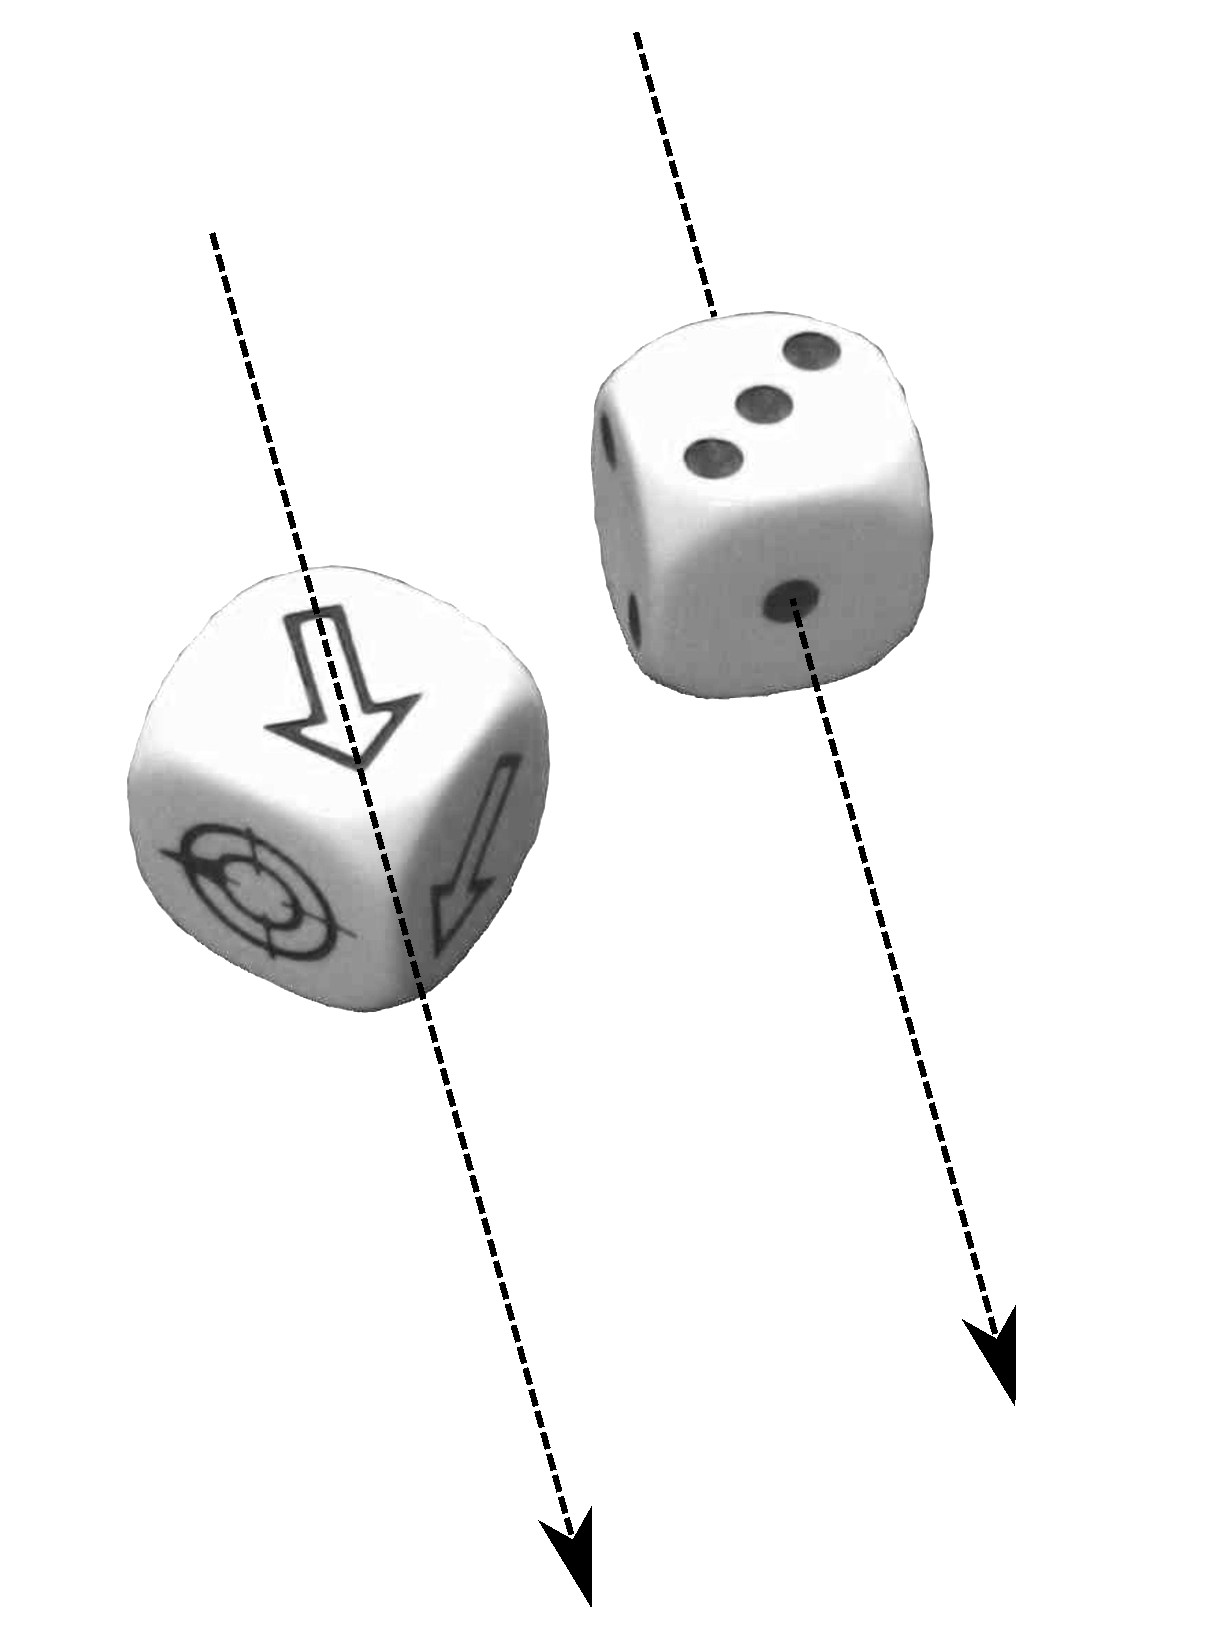
\includegraphics[width=4cm]{pics/deviation_dice.png}
\caption{Deux façons équivalentes de représenter un Dé de Direction.}
\label{figure/deviation_dice}
\end{figure}


%
%\newpage
%
\part{Logistique du champ de bataille}

\section{Mesurer les distances}

L'unité de mesure dans Batailles Fantastiques : Le 9\ieme{} Âge est le pouce, noté \distance{}. Il vaut 2,54 {\centi\meter} exactement. Toutes les distances et portées sont indiquées et mesurées en pouces. Pour déterminer la distance entre deux objets sur le champ de bataille, comme des unités, décors ou autres éléments, vous devez toujours mesurer entre les points au sol les plus proches des deux objets, même si cela traverse un quelconque obstacle. Entre deux figurines, les mesures se font donc bout de socle à bout de socle.

Les règles se réfèrent souvent à des objets étant à moins d'une certaine distance. Dans ce cas, mesurez la distance entre leurs points les plus proches de ces objets. Si cette distance est inférieure à la portée donnée, les objets sont considérés comme étant à portée. Notez que cela signifie qu'une figurine est toujours à portée d'elle-même et qu'une figurine ou une unité n'a pas besoin d'être entièrement à portée, une partie de celle-ci suffit.
 
\textbf{Les joueurs sont autorisés à mesurer n'importe quelle distance à tout moment.}

\section{Ligne de Vue}

\newfromWHB{Une figurine a une Ligne de Vue sur sa cible (point ou unité) si vous pouvez tracer une ligne droite depuis l'avant de son socle directement jusqu'à la cible, sans sortir de l'arc frontal de la figurine, et sans être bloqué par un Décor Occultant ou par le socle d'une figurine qui a une Taille \textbf{plus grande que la figurine et sa cible à la fois}.} Une figurine d'un rang arrière peut avoir les mêmes Lignes de Vue que la figurine du premier rang de la ou des même(s) colonne(s). On considère qu'une unité a une Ligne de Vue sur une cible si une ou plusieurs figurines de l'unité ont une Ligne de Vue sur cette cible. \newfromWHB{Les figurines d'une unité ne bloquent jamais les Lignes de Vue des autres figurines de cette unité.}

\subsection{Taille des figurines}
\label{modelheight}

\newfromWHB{Les figurines peuvent avoir trois Tailles :}

\noindent\textbf{Petite}

\newfromWHB{Toute figurine étant du type de troupe \infantry{}, \warbeast{}, \swarm{} ou \warmachine{}.}

\noindent\textbf{Moyenne}

\newfromWHB{Toute figurine étant du type de troupe \cavalry{}, \monstrousinfantry{}, \monstrouscavalry{}, \monstrousbeast{} ou \chariot{}.}

\noindent\textbf{Grande}

\newfromWHB{Toute figurine ayant la règle \largetarget{}.}


\section{Règle du Pouce d'Écart}

Dans des circonstances habituelles, les unités doivent toujours laisser un espace d'au moins \distance{\textbf{1}} entre elles, alliées ou ennemies, et avec les Terrains Infranchissables. \newfromWHB{Pendant un déplacement, cette distance est réduite à \textbf{0,5}\distance{}, mais à la fin du mouvement, l'écart d'un pouce doit être respecté.}

Quelques déplacements spéciaux autorisent une entorse à la Règle du Pouce d'Écart, comme les charges, qui permettent aux unités d'engager des Corps à Corps. D'autres types de déplacement permettent à une unité de se rapprocher à moins d'\distance{1} d'unités alliées ou de Terrains Infranchissables, mais seul un mouvement de charge permet le contact avec des unités ennemies. Si une unité est temporairement autorisée à ne pas respecter la Règle du Pouce d'Écart, elle peut l'ignorer par rapport à l'unité ou au Terrain Infranchissable aussi longtemps qu'elle reste à moins de \distance{1}. Elle ne peut cependant jamais entrer en contact socle à socle avec une unité ennemie qu'elle n'a pas chargée. Une fois que l'écart d'un pouce est à nouveau respecté, la règle recommence automatiquement à s'appliquer.

\section{Bords de table}

Les bords de table correspondent aux limites du jeu. Les figurines peuvent se retrouver temporairement en dehors de cette limite durant un déplacement, du moment que pas plus de la moitié du socle d'une figurine ne dépasse à n'importe quel moment, et tant qu'aucune partie de la figurine ne se retrouve en dehors à la fin du déplacement. Les Gabarits peuvent être placés partiellement en dehors du champ de bataille et affectent toujours les figurines sous la partie du Gabarit toujours sur le champ de bataille.


%
%\newpage
%
\part{Caractéristiques}

\section{Profil de Caractéristiques}

Chaque figurine possède un Profil, qui est composé de neuf caractéristiques présentée dans la table \ref{table/characteristics}.

\begin{table}[!htbp]
\centering
\begin{tabular}{M{0.6cm}M{2.8cm}M{12cm}@{}}
\hline
\textbf{M} & Mouvement & \flufffont{La vitesse à laquelle la figurine se déplace, en pouces par tour.} \tabularnewline
\textbf{CC} & Capacité de Combat & \flufffont{Détermine les chances de toucher et d'éviter d'être touché au Corps à Corps.} \tabularnewline
\textbf{CT} & Capacité de Tir & \flufffont{Détermine les chances de toucher avec des armes de Tir.} \tabularnewline
\textbf{F} & Force & \flufffont{Plus la Force est élevée, plus il est facile de blesser et de passer à travers l'armure.} \tabularnewline
\textbf{E} & Endurance & \flufffont{Une grande Endurance permet d'encaisser les coups plus facilement.} \tabularnewline
\textbf{PV} & Points de Vie & \flufffont{Quand une figurine perd tous ses Points de Vie, elle est retirée comme perte.} \tabularnewline
\textbf{I} & Initiative & \flufffont{Une plus grande Initiative permet de frapper en premier.} \tabularnewline
\textbf{A} & Attaques & \flufffont{Le nombre d'attaques qu'une figurine peut porter au Corps à Corps en une Manche.} \tabularnewline
\textbf{Cd} & Commandement & \flufffont{Mesure de la discipline et de la capacité à rester au combat dans des situations dangereuses.} \tabularnewline
\hline
\end{tabular}
\caption{\label{table/characteristics}Les Caractéristiques d'une figurine.}
\end{table}


Toutes les caractéristiques vont de 0 à 10 et ne peuvent jamais dépasser ces valeurs.

\noindent\textbf{Caractéristique à 0}

Quand la valeur d'une Caractéristique est égale à 0, cela peut être représenté par un tiret \og - \fg{} ou par une étoile \og \starsymbol{} \fg{}.

\noindent CC à 0 : La figurine est touchée automatiquement au Corps à Corps et ne peut toucher au Corps à Corps que sur un \result{6}.

\noindent CT à 0 : La figurine ne peut pas utiliser d'Arme de Tir.

\noindent F à 0 : Les attaques de la figurine ne peuvent pas blesser.

\noindent E à 0 : Les jets pour blesser dirigés contre la figurine réussissent sur 2+.

\noindent PV à 0 : La figurine est retirée comme perte.

\noindent A à 0 : Un élément de figurine dont la Caractéristique d'Attaques non modifiée est à 0 ne peut pas porter d'attaque au Corps à Corps.

\section{Test de Caractéristique}

Quand une figurine doit passer un Test de Caractéristique, lancez 1D6. Si le résultat est \result{6} ou s'il est strictement plus grand que la Caractéristique testée, le test est raté. Sinon, le test est réussi. Ainsi, les figurines avec une Caractéristique à 0 échoueront automatiquement tout Test lié à cette Caractéristique.

Quand une figurine doit passer un Test de Caractéristique et qu'elle possède plusieurs valeurs pour une même Caractéristique, comme un cheval et son cavalier, faites un test unique pour la figurine entière en utilisant la Caractéristique la plus haute. Quand un Test de Caractéristique doit être passé pour toute une unité, prenez la valeur la plus grande de l'unité.

\subsection{Caractéristique non modifiée}

Une Caractéristique non modifiée est la valeur de la Caractéristique qui peut être lue sur le profil de la figurine, en ignorant tous les équipements, sorts et règles l'affectant. Les seules exceptions sont les changements de Caractéristique appliqués lors de la construction de l'armée, comme par exemple en améliorant une figurine en \og Vétéran \fg{}, lui donnant +1 en Force. Ce type de modification est considéré comme faisant partie de la Caractéristique non modifiée de la figurine.

\subsection{Caractéristique Empruntée}
\label{borrowed_characteristics}

Dans certains cas,  une figurine peut emprunter ou utiliser la Caractéristique d'une autre figurine. La valeur de la Caractéristique est empruntée après toute modification venant de l'équipement, de sorts ou de règles spéciales affectant la figurine propriétaire. Les modifications liées à la figurine qui emprunte la caractéristique sont ensuite appliquées, en suivant les règles de priorité des modificateurs du paragraphe \ref{priority_of_modifiers} ci-dessous.

\subsection{Test de Commandement}

Un test de Commandement se passe en lançant 2D6 et en comparant le résultat avec la valeur de la Caractéristique de Commandement de la figurine. Si le résultat est strictement plus grand que le Commandement de la figurine, le test est raté. Sinon, le test est réussi. \newfromWHB{Si une unité dispose de plusieurs valeurs de Commandement quand elle doit passer un test, par exemple si un Personnage a rejoint l'unité, le propriétaire peut choisir la valeur à utiliser.}

Il y a beaucoup d'occasions différentes de tester le Commandement, comme les tests de Panique ou de Moral. Ces tests restent des tests de Commandement, peu importe les modificateurs et règles spéciales associés.

\subsection[Priorité des modificateurs]{\newfromWHB{Priorité des modificateurs}}
\label{priority_of_modifiers}

Quand une Caractéristique est modifiée, les modificateurs s'appliquent dans un ordre précis :
\begin{enumerate}
\item Caractéristique empruntée* ou fixée à une certaine valeur, comme par la \inspiringpresence{}, ou après un test de \fear{} raté.
\item Multiplicateurs, comme une division par deux, une Caractéristique doublée ou triplée. À moins que le contraire ne soit précisé, arrondissez toujours au supérieur.
\item Additions et soustractions, comme -1 ou +3.
\end{enumerate}
\noindent * Si la Caractéristique à emprunter est modifiée, appliquer ces modifications avant d'emprunter la Caractéristique. 

Si plusieurs modificateurs de la même étape doivent être appliqués, commencez par appliquer les modificateurs sans précision de valeur minimale ou maximale, puis ceux avec de telles précisions, comme \og -1 en Initiative jusqu'à un minimum de 1 \fg{}. Ensuite, appliquez les modificateurs dans l'ordre chronologique. Rappelez-vous qu'une Caractéristique ne peut jamais être modifiée, même temporairement, de façon à dépasser 10 ou tomber en dessous de 0.


%
%\newpage
%
\part{Préparer une partie}

\section{Construire votre Liste d'Armée}
\label{building_an_army}

Batailles Fantastiques : Le 9\ieme{} Âge propose une série de Livres d'Armée qui décrivent les spécificités de chaque armée. Chaque armée regroupe un ensemble unique de personnages, troupes et règles. Les \textbf{Personnages} sont répartis entre Seigneurs et Héros, et les \textbf{Troupes} entre unités de Base, unités Spéciales et unités Rares.

\noindent\hspace*{\fill} \begin{minipage}[t]{0.3\textwidth}
\begin{center}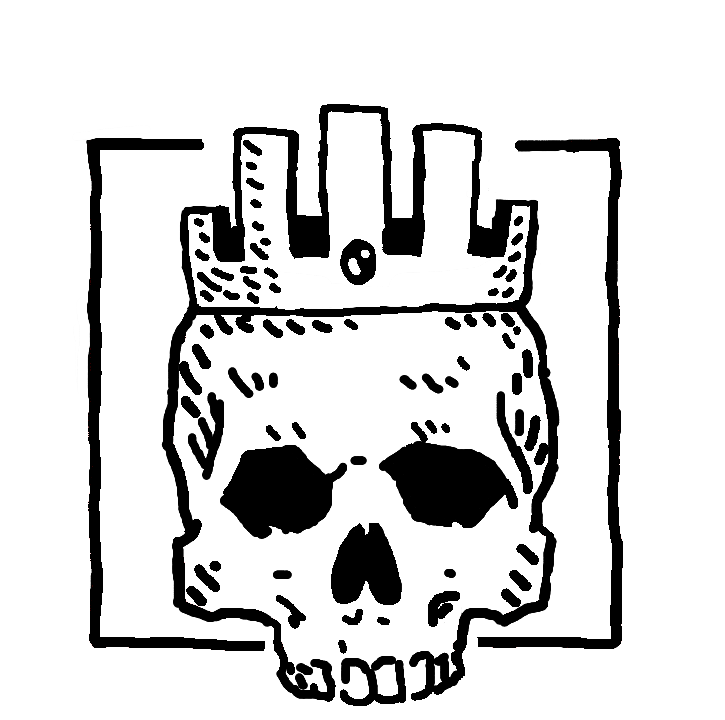
\includegraphics[width=2.5cm]{../Layout/pics/logo_lord.png}

Les Seigneurs sont les individus les plus puissants d'une armée.
\end{center}
\end{minipage}\hspace*{1cm}
\begin{minipage}[t]{0.3\textwidth}
\begin{center}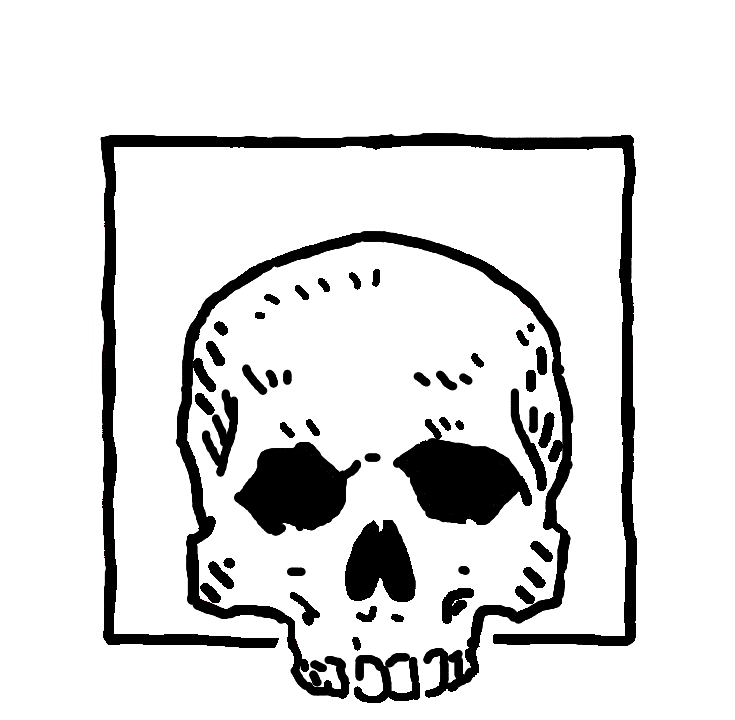
\includegraphics[width=2.5cm]{../Layout/pics/logo_hero.png}

Les Héros sont des individus exceptionnels.
\end{center}
\end{minipage}\hspace*{\fill}

\noindent\begin{minipage}[t]{0.3\textwidth}
\begin{center}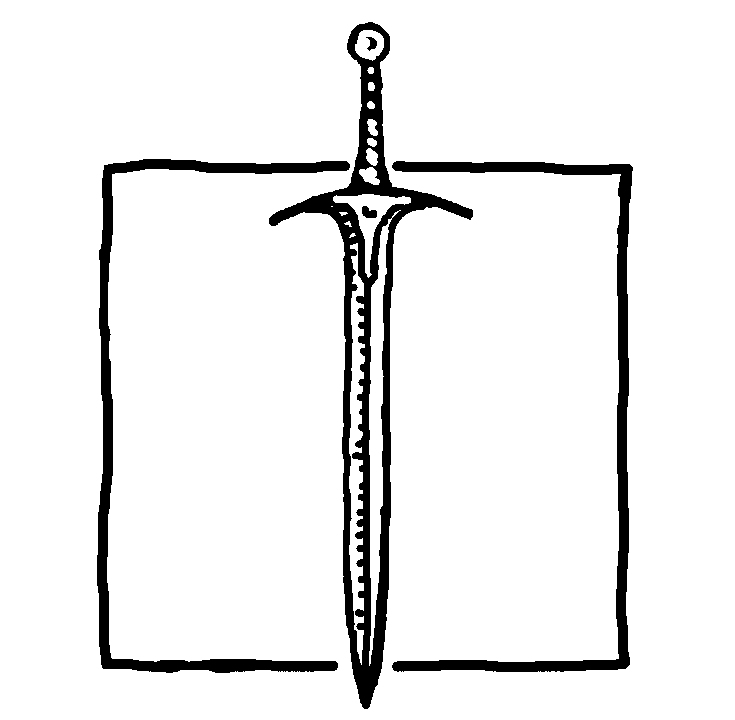
\includegraphics[width=2.5cm]{../Layout/pics/logo_core.png}

Les unités de Base représentent les guerriers les plus communs de l'armée.
\end{center}
\end{minipage}\hfill
\begin{minipage}[t]{0.3\textwidth}
\begin{center}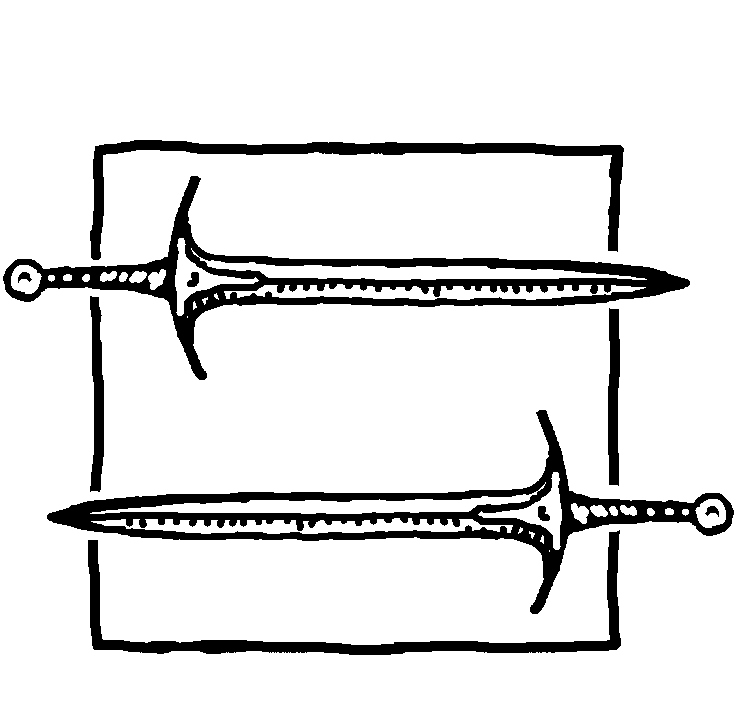
\includegraphics[width=2.5cm]{../Layout/pics/logo_special.png}

Les vétérans et régiments d'élite constituent les unités Spéciales.
\end{center}
\end{minipage}\hfill
\begin{minipage}[t]{0.3\textwidth}
\begin{center}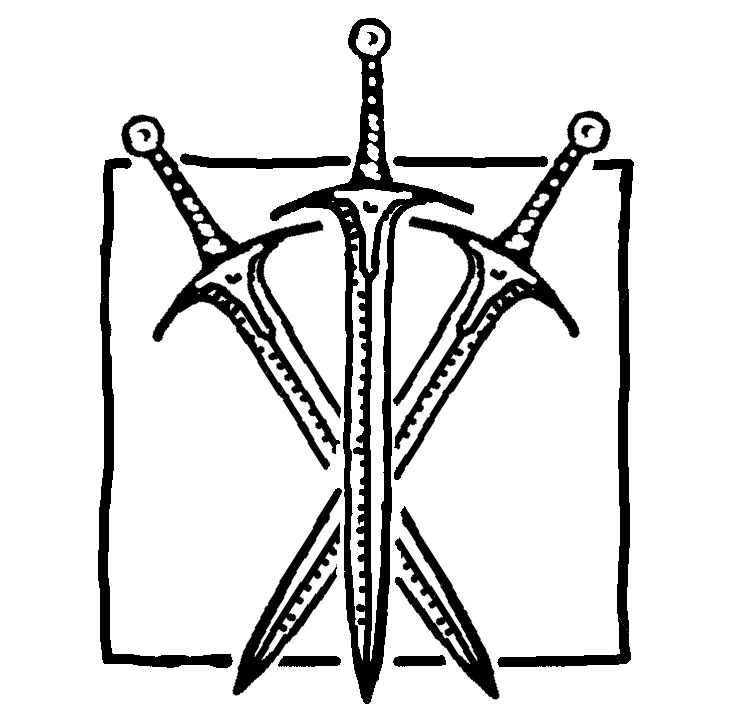
\includegraphics[width=2.5cm]{../Layout/pics/logo_rare.png}

Les unités Rares sont des troupes extraordinaires, des monstres peu communs et des machines de guerre inhabituelles.
\end{center}
\end{minipage}

\vspace*{10pt}
La première étape de la construction d'une armée est d'écrire un choix d'unités, leurs options et leurs Coûts en Points sur un document qu'on appelle \og Liste d'Armée \fg{}. La composition d'une liste est sujette à des règles et restrictions, que l'on décrit en détails dans la suite du chapitre.

\subsection{Coût en points}

Chaque unité, arme, amélioration, Objet Magique, etc. vaut un certain montant de points. Le Coût en Points d'une unité est la somme des Coûts en Points de chacune de ses figurines et des options. Le Coût en Points d'une armée est la somme des Coûts en Points de toutes ses unités.

\paragraph{\newfromWHB{Demi-point}}

La valeur en points d'une unité doit être entière. Si une amélioration coûte 0,5 point, le coût final de l'unité est arrondi à la valeur supérieure.

\paragraph{\newfromWHB{Coûts Seigneur / Héros}}

Si le coût d'une option ou d'un objet magique est écrit avec un \og / \fg{}, par exemple 50 / 40 pts, la première valeur est le coût pour un Seigneur tandis que la seconde s'applique pour un Héros ou un Champion.

\section{Restrictions}

Une armée de Batailles Fantastiques : Le 9\ieme{} Âge doit suivre des règles simples de composition, détaillées ci-dessous :

\begin{itemize}[label={\textbullet}]
\item \textbf{Coût en Points de l'armée}\newline
Le Coût en Points de l'armée, combinant la valeur de toutes les unités, équipements et options, ne doit pas dépasser la limite en points décidée pour la partie. Elle peut cependant descendre jusqu'à 20 points en dessous de cette limite.

\item \textbf{Catégories d'unités}\newline
Les unités sont regroupées en 5 Catégories. Le nombre de points que l'on peut dépenser dans chaque groupe dépend de la Catégorie. De plus, une même entrée du livre d'armée ne peut être prise qu'un certain nombre de fois. Ces informations sont résumées dans la table \ref{table/unitcategories} ci-dessous.

\begin{table}[!htbp]
\centering
\begin{tabular}{rcc}
\hline
 & \textbf{Limite de points} & \textbf{Limite de duplication} 			\tabularnewline
\textbf{Base} 					& min. 25 \% 			& \newfromWHB{max. 4} 	\tabularnewline
\textbf{Spécial} 				& - 					& max. 3 			\tabularnewline
\textbf{Rare} 					& max. 25 \% 			& max. 2 			\tabularnewline
\textbf{Héros} 					& max. \newfromWHB{50 \%} 	& \newfromWHB{max. 3} 	\tabularnewline
\textbf{Seigneurs} 			& max. \newfromWHB{35 \%} 	& \newfromWHB{max. 3} 	\tabularnewline
\textbf{Héros + Seigneurs} & max. 50 \% 			& - 				\tabularnewline
\hline
\end{tabular}
\caption{\label{table/unitcategories}Restrictions de composition d'armée.}
\end{table}

\newfromWHB{Parfois, certaines unités peuvent être déplacées d'une Catégorie à une autre. Par exemple, certaines règles peuvent autoriser un joueur à prendre un Char comme choix de Base plutôt qu'en choix Spécial. Dans de tels cas, il faut respecter à la fois la limite de duplication de son ancienne Catégorie et de sa nouvelle. La limite de points compte, quant à elle, seulement dans la nouvelle catégorie. Dans notre exemple précédent, vous ne pouvez pas inclure plus de 3 Chars dans votre armée, mais ceux-ci compteront dans les 25 \% d'unités de Base nécessaires.}

\item \textbf{Taille d'armée minimale}\newline
\newfromWHB{Une armée doit contenir au moins 4 unités sans compter les Personnages. On ne peut comptabiliser qu'une seule unité de type Machine de Guerre pour atteindre ce minimum.}
\item \textbf{Le Général}\newline
Un des Personnages de l'armée doit être nommé Général. Il faut donc qu'il y ait au moins un Personnage dans l'armée capable de tenir ce rôle. Une armée ne peut comporter qu'un seul Général.
\item \textbf{\newfromWHB{\oneofakind{} et \oneperarmy}}\newline
Les unités, options et objets marqués \oneofakind{} ou \oneperarmy{} ne peuvent être pris qu'une fois par armée. Ceux marqués \oneofakind{} peuvent être pris en deux exemplaires dans une Grande Armée.
\item \textbf{\newfromWHB{\zerotoXchoice{X}}}\newline
Certaines unités disposent d'une limite de duplication différente notée \zerotoXchoice{X}, par exemple \zerotoXchoice{2}. Cela signifie que ces unités peuvent être prises entre 0 et X fois, en ignorant les limites de duplication classiques. La limite maximale X est divisée par 2 pour une Patrouille en arrondissant à l'unité supérieure, et multipliée par 2 pour une Grande Armée.
\end{itemize}

\newpage
\section{Patrouilles et Grandes Armées}

Les règles de composition d'armée peuvent être modifiées selon la limite en points de la partie, si les armées sont plus petites ou grandes que la norme.

\begin{multicols}{2}\raggedcolumns

\begin{center}\textbf{\newfromWHB{Patrouilles}}\end{center}

Les armées de 1500 points ou moins sont appelées Patrouilles. La taille d'armée minimale est réduite à 3 unités. La table suivante donne les nouvelles limites de duplication :

\begin{center}
\begin{tabular}{rp{3.8cm}}
\hline
\textbf{Base} 							& max. 2 \tabularnewline
\textbf{Spécial} 						& max. 2 \tabularnewline
\textbf{Rare} 							& max. 1 \tabularnewline
\textbf{Héros et Seigneurs}	& max. 2 \tabularnewline
\textbf{\oneofakind}			    & max. 1 \tabularnewline
\textbf{\oneperarmy}				& max. 1 \tabularnewline
\textbf{\zerotoXchoice{X}} 	& divisée par 2,\newline arrondie au supérieur \tabularnewline
\hline
\end{tabular}
\end{center}

\columnbreak

\begin{center}\textbf{\newfromWHB{Grandes Armées}}\end{center}

Les armées de 4000 points ou plus sont appelées Grandes Armées. Les unités marquées \oneofakind{} peuvent être prises en deux exemplaires. La table suivante donne les nouvelles limites de duplication :

\begin{center}
\begin{tabular}{rl}
\hline
\textbf{Base} 							& max. 8 \tabularnewline
\textbf{Spécial} 						& max. 6 \tabularnewline
\textbf{Rare} 							& max. 4 \tabularnewline
\textbf{Héros et Seigneurs}	& max. 6 \tabularnewline
\textbf{\oneofakind}			    & max. 2 \tabularnewline
\textbf{\oneperarmy}				& max. 1 \tabularnewline
\textbf{\zerotoXchoice{X}} 	& doublée \tabularnewline
\hline
\end{tabular}
\end{center}
\end{multicols}

\newpage
\section{Liste d'Armée ouverte ?}

Les règles de ce jeu ont été équilibrées avec l'idée de listes d'armée complètement révélées. Par exemple, votre adversaire doit savoir quels Objets Magiques vos figurines possèdent. Nous encourageons les joueurs à partager leur Liste d'Armée complète avec leur adversaire au début de la partie, en détaillant unités, options, Objets Magiques, capacités spéciales, coûts en points, etc. Les seules choses qui ne doivent pas être montrées à votre adversaire sont celles explicitement citées comme cachées ou secrètes, comme par exemple dans quelle unité un Assassin est caché. Précisons que l'Assassin et son équipement sont quand même mentionnés dans la liste.

\subsection[Règles optionnelles pour listes cachées]{\newfromWHB{Règles optionnelles pour listes cachées}}
\label{hidden_lists}

Certains joueurs peuvent préférer jouer avec des listes dites \og cachées \fg{}. Rappelons que les règles du jeu n'ont pas été équilibrées dans cette optique. Dans ce cas, nous vous proposons de suivre les règles suivantes. La plus grande partie de votre armée doit rester connue de votre adversaire avant le début de la partie. Seuls quelques aspects sont secrets, ou \og cachés \fg{}. Les deux joueurs peuvent donner à leur adversaire une liste simplifiée dans laquelle les détails cachés sont omis.

Voilà les éléments qui peuvent être cachés : 

\begin{itemize}[label={-}]
\item Les Objets Magiques pris dans la liste commune de ce livre.
\item Les Objets Magiques spécifiques aux Livres d'Armée ainsi que toute option suivant les règles des Objets Magiques, comme les Objets Démoniaques et les Runes Naines.
\end{itemize}

Le reste doit être présenté dans la partie ouverte de votre liste. De plus, les Objets Magiques et assimilés qui ont un équivalent standard doivent être présentés sur la liste ouverte comme tels. Une Arme Lourde magique, par exemple, apparait comme une simple Arme Lourde.

Quand vous possédez au moins deux unités qui sont identiques dans la liste ouverte, mais qui ont une différence cachée, comme par exemple une Bannière Magique, vous devez avoir un moyen visible de les différencier, noté sur votre liste complète. Par exemple, la bannière rouge est la Bannière Magique, tandis que la bleue est ordinaire.

\paragraph{Révéler les Objets Magiques}

Un Objet Magique, ou équivalent, doit être révélé à la première utilisation. Un objet est considéré comme utilisé quand il a une chance d'affecter le jeu d'une quelconque façon. Entre autres :
\begin{itemize}[label={-}]
\item si cela affecte un jet de dé, même si le résultat obtenu sur le dé ne déclenche pas d'effet ;
\item si cela altère une attaque, via une Arme Magique ou tout objet dont une règle affecte l'attaque ;
\item si cela altère un jet de sauvegarde. L'objet doit alors être révélé avant que les dés ne soient jetés. Remarquez qu'un objet qui affecte une sauvegarde de la même manière que son équivalent standard le ferait, comme un Bouclier Magique, ne doit pas forcément être révélé.
\end{itemize}

Un objet qui augmente la mobilité ne compte comme étant utilisé que lorsque l'unité se déplace plus loin qu'elle ne le pourrait sans l'objet, ou lorsqu'elle charge. Déclarez alors l'objet avant de lancer le jet de distance de charge, mais après que les réactions ont été déclarées. Pour les Objets Runiques Nains, ne révélez que la Rune qui est utilisée, pas la combinaison complète.


%
%\newpage
%
\part{Séquence Pré-Partie}

Il y a plusieurs étapes à suivre dans un certain ordre afin de mettre en place une partie de Batailles Fantastiques : Le 9\ieme{} Âge. L'ensemble de ces étapes est appelé Séquence Pré-Partie. La première étape, et la plus importante, est de trouver un adversaire motivé et de vous mettre d'accord sur la taille de la partie. Les joueurs peuvent ensuite se dévoiler leurs Listes d'Armée et commencer à installer le champ de bataille. Puis ils déterminent le type de déploiement, les Objectifs Secondaires, les zones de déploiement et génèrent les sorts des \wizards{}. La dernière étape consiste à passer à ce qu'on appelle le Déploiement.

Voilà un résumé des étapes de la séquence pré-partie :

\hspace*{0.3cm}
\begin{tabular}{c|l}
1 & Décidez de la taille de la partie. \tabularnewline
2 & Montrez-vous vos Listes d'Armée. \tabularnewline
3 & Installez le champ de bataille. \tabularnewline
4 & Tirez au sort le type de déploiement. \tabularnewline
5 & Tirez au sort les Objectifs Secondaires. \tabularnewline
6 & Déterminez les zones de déploiement. \tabularnewline
7 & Générez les sorts. \tabularnewline
8 & Phase de Déploiement. \tabularnewline
\end{tabular}

\hypertarget{gamesize}{\subsection{Taille de la partie}}

Les deux armées qui se font face doivent avoir à peu près le même coût en points, afin que l'issue de la bataille dépende des stratégies et tactiques rusées des joueurs plutôt que d'une asymétrie dans la puissance des armées. Les deux joueurs doivent donc se mettre d'accord sur le coût en points des armées que chacun commandera, déterminant ainsi la taille de la partie. Des armées de 1500 à 3000 points correspondent à des petites escarmouches. De 3000 à 6000 points, la bataille commence à être plus importante. Au delà de 6000 points, le jeu met en scène un conflit massif entre des armées épiques. Nous recommandons une taille de partie autour de 4500 points pour profiter du meilleur équilibre du jeu.

\hypertarget{sharearmylist}{\subsection{Dévoiler les listes}}

Après avoir décidé de la taille de la partie, l'étape suivante est d'échanger les Listes d'Armée ainsi que toute information pertinente à propos de la partie à venir. Les joueurs peuvent aussi choisir de garder quelques aspects de leur armée secrets et de ne les révéler qu'au fur et à mesure de la partie, comme expliqué dans le paragraphe \ref{hidden_lists}.

\newpage
\hypertarget{buildbattlefield}{\subsection{Installer le champ de bataille}}

La partie se joue habituellement sur un champ de bataille de \distance{48} par \distance{72} (environ 1,20 {\meter} par 1,80 {\meter}). Pour de plus petites batailles, au format Patrouille, nous recommandons une table de \distance{36} par \distance{48} (environ 90 {\centi\meter} par 1,20 {\meter}) et pour les plus grandes parties, au format Grande Armée, ajustez le champ de bataille à la taille des armées. Bien qu'une partie puisse être jouée sur une table vierge, on y place habituellement quelques Décors. Les joueurs peuvent tout à fait se mettre d'accord sur le nombre, le type, la taille et la position des Décors. Sinon, voilà les règles standard pour générer un champ de bataille aléatoire :

\begin{itemize}[label={\textbullet}]
\item Divisez la table de jeu en sections de \distance{24} par \distance{24}, soit environ 60 {\centi\meter} par 60 {\centi\meter}. Si la table fait \distance{36} par \distance{48}, prenez plutôt des sections de \distance{18} par \distance{24}, soit environ 45 {\centi\meter} par 60 {\centi\meter}.

\item Placez chacun des trois Décors suivants au centre de sections choisies aléatoirement, avec un Décor au plus dans chaque section : un Bâtiment ou un Terrain Infranchissable (tirez au hasard), une Colline et une Forêt. Déplacez ensuite chaque Décor de \distance{2D6} dans une direction aléatoire.

\item Ajoutez 2D3 Décors (1D3 si la table fait \distance{36} par \distance{48}), en suivant les règles ci-dessus pour leur positionnement. Lancez 1D6 pour déterminer le type de chaque Décor additionnel :
\begin{enumerate}
\item Colline
\item Forêt
\item Champ
\item Eau peu profonde
\item Mur
\item Ruines
\end{enumerate}

\item Tous les Décors doivent être placés au moins à \distance{6} les uns des autres. Bougez-les aussi peu que possible de leur position initiale pour satisfaire à cette condition. Si cela n'est pas possible, retirez le Décor qui pose problème.

\item Nous vous recommandons des tailles de Décor comprises entre \distance{6} par \distance{8} (soit 15x20 {\centi\meter}) et \distance{6} par \distance{10} (15x25 {\centi\meter}), excepté pour les Murs pour lesquels nous conseillons \distance{1} par \distance{10} (2,5x25 {\centi\meter}).
\end{itemize}


\newpage
\hypertarget{deploymenttype}{\subsection{Type de déploiement}}

\hypertarget{deploymenttypefigure}{%
Tirez au hasard le type de déploiement en lançant 1D6 :
}

\hypertarget{frontlineclash}{\paragraph{1-2 : \frontlineclash{}}}
\label{figure/deployment}
\begin{minipage}[c]{0.35\textwidth}
\def\svgwidth{\textwidth}
\input{pics/deployment_one.pdf_tex}
\end{minipage}\hfill
\begin{minipage}[c]{0.62\textwidth}
La table est divisée en deux moitiés égales par une ligne centrale, dans le sens de la longueur. Les zones de déploiement commencent à \distance{12} de part et d'autre de cette ligne et s'étendent au delà. 
\end{minipage}

\hypertarget{refusedflank}{\paragraph{3-4 : \refusedflank{}}}

\begin{minipage}[c]{0.35\textwidth}
\def\svgwidth{\textwidth}
\input{pics/deployment_two.pdf_tex}
\end{minipage}\hfill
\begin{minipage}[c]{0.62\textwidth}
La table est divisée en deux moitiés par une diagonale de la table. Le joueur choisissant sa zone de déploiement décide de la diagonale à utiliser. Les zones de déploiement commencent à \distance{9} de part et d'autre de cette ligne et s'étendent au delà.
\end{minipage}

\hypertarget{encircle}{\paragraph{5 : \encircle{}}}

\newcommand{\deploymentfigAttacker}{\flufffont{Attaquant}}
\newcommand{\deploymentfigDefender}{\flufffont{Défenseur}}
\begin{minipage}[c]{0.35\textwidth}
\def\svgwidth{\textwidth}
\input{pics/deployment_three.pdf_tex}
\end{minipage}\hfill
\begin{minipage}[c]{0.62\textwidth}
La table est divisée en deux moitiés égales par une ligne centrale, dans le sens de la longueur. Le joueur choisissant sa zone de déploiement décide s'il veut être l'attaquant ou le défenseur. L'attaquant peut se déployer à plus de \distance{9} de la ligne centrale à plus du quart des bords courts de la table (\distance{18} sur une table de \distance{72} de long) et à plus de \distance{15} de la ligne médiane aux deux autres endroits, près des bords courts. Le défenseur fait le contraire : les limites de \distance{9} et \distance{15} sont inversées.
\end{minipage}

\hypertarget{counterthrust}{\paragraph{6 : \counterthrust{}}}

\begin{minipage}[c]{0.35\textwidth}
\def\svgwidth{\textwidth}
\input{pics/deployment_four.pdf_tex}
\end{minipage}\hfill
\begin{minipage}[c]{0.62\textwidth}
La table est divisée en deux moitiés égales par une ligne centrale, dans le sens de la longueur. Les zones de déploiement commencent à \distance{6} de part et d'autre de cette ligne et s'étendent au delà. Aucune unité ne peut être déployée à moins de \distance{18} d'une unité ennemie. Cela ne concerne pas les unités au déploiement spécial comme celles avec la règle \scout{}.

Les joueurs ne peuvent déployer qu'une seule unité par tour de déploiement, et posent donc une unité tour à tour. L'ensemble des Personnages et l'ensemble des Machines de Guerre comptent chacun comme une seule unité en terme de déploiement.
\end{minipage}


\newpage
\hypertarget{secondaryobjectives}{\subsection{Objectifs Secondaires}}

Avant de choisir les zones de déploiement, tirez au hasard un Objectif Secondaire en lançant 1D6 :

\paragraph{1-2 : Tenez la Ligne}

\flufffont{Tenez et défendez le centre du champ de bataille.}\newline
Placez un marqueur sur le centre du champ de bataille au besoin.

\paragraph{3-4 : Percée}

\flufffont{Envahissez le territoire ennemi.}\newline
Marquez la position des zones de déploiement.

\paragraph{5 : Capturez les Étendards}

\flufffont{Les cibles de valeur doivent être annihilées.}\newline
Après avoir déplacé les unités avec la règle \vanguard{} et avant de déterminer qui aura le premier Tour de Joueur, les deux joueurs doivent désigner chacun leur tour et ouvertement une unité ennemie avec la règle \scoring{}, jusqu'à en avoir choisi trois ou toutes les unités éligibles s'il y en a moins de trois. Les unités qui n'ont pas encore été déployées, comme les unités avec la règle \ambush{}, peuvent être désignées. Le joueur qui a fini de se déployer en premier commence à choisir.

\paragraph{6 : Sécurisez la Cible}

\flufffont{Des ressources cruciales ne doivent pas tomber entre les mains de l'ennemi.}\newline
Après avoir choisi les zones de déploiement, chaque joueur place un marqueur sur le champ de bataille, en commençant par celui qui a choisi sa zone de déploiement. Ces marqueurs doivent être positionnés à plus de \distance{12} de la zone de déploiement du joueur qui le place, et à plus de \distance{24} l'un de l'autre.

Référez-vous au chapitre \ref{scoring_and_victory_conditions} (page \pageref{scoring_and_victory_conditions}) pour plus de détails sur la capture d'un objectif et l'impact sur les Points de Victoire.

\hypertarget{deploymentzones}{\subsection{Zones de déploiement}}

Tirez au hasard afin de déterminer qui choisit les zones de déploiement. Par exemple, un joueur peut lancer 1D6 : sur 4+, c'est lui qui choisit. En cas de \frontlineclash{} ou de \counterthrust{}, il s'approprie un des bords longs du champ de bataille Pour un \refusedflank{}, il peut prendre un des quatre coins. Enfin, pour un \encircle{}, il choisit le côté et s'il est l'attaquant ou le défenseur.

\newpage
\hypertarget{generatespells}{\subsection{Générer les sorts}}
\label{generating_spells}

Chaque joueur génère les sorts pour tous ses \wizards{}, en commençant par le joueur qui a choisi sa zone de déploiement. Pour cela, sélectionnez un \wizard{} et consultez sa Voie de Magie, qui doit être inscrite sur la Liste d'Armée. Toutes les Voies de Magie peuvent être trouvées dans le Livre de Magie.

\paragraph{Sorts numérotés de 1 à 6}

Toutes les Voies de Magie comprennent des \og \learnedspells{} \fg{}, numérotés de 1 à 6. Lancez autant de D6 que de sorts que le \wizard{} connaît pour voir quels sorts il pourra utiliser lors de cette bataille. Si un \result{1} est obtenu, le \wizard{} connaît le sort numéro 1, et ainsi de suite. Si un \learnedspell{} est obtenu deux fois, parce que les dés donnent un double ou parce qu'un autre \wizard{} de la même armée a déjà choisi ce sort, le sort en double doit être remplacé par un autre sort de son choix de la même Voie de Magie qui n'a pas encore été choisi.

\paragraph{Sorts numérotés 0}

Certaines Voies de Magie comprennent un sort numéroté 0. C'est un type spécial de \learnedspell{}. Tout \wizard{} peut échanger un de ses \learnedspells{} de la même Voie contre ce sort. Notez qu'il ne peut pas être dupliqué au sein d'une armée.

Deux \wizards{} de la même armée ne peuvent pas connaître le même \learnedspell{} et aucun \wizard{} ne peut disposer d'un \learnedspell{} en plusieurs exemplaires. S'il est impossible de remplacer un \learnedspell{} en double par un autre, le sort est perdu. Les sorts qui ne sont pas générés en suivant ces règles, comme les sorts prédéterminés ou les \boundspells{}, sont ignorés pour la duplication des sorts. De tels sorts peuvent ainsi être présents plus d'une fois dans une même armée.

\paragraph{Sorts numérotés \og \attributespellnumber{} \fg{} ou \og \traitspellnumber{} \fg{}}

Certaines Voies de Magie comprennent des sorts numérotés \og \attributespellnumber{} \fg{} ou \og \traitspellnumber{} \fg{}. Ce sont des sorts spéciaux appelés respectivement \attributespells{} et \traitspells{}. Tout \wizard{} connaissant au moins un \learnedspell{} d'une Voie connaît aussi l'\attributespell{} et/ou le \traitspell{} de la même Voie en plus de ses autres sorts.

%
%\newpage
%% Base sur la VO 0.11.9
% Relecture technique: 
% Relecture syntaxique: 

\part[Déploiement]{\nouveau{Déploiement}}

\subsection*{Étapes du déploiement}

Le déploiement suit les étapes décrites dans la table \ref{table/etapes_deploiement}.

\begin{table}[!htbp]
\centering
\begin{tabular}{c|l}
\textbf{1} & \nouveau{Déterminez qui commence à se déployer}. \tabularnewline
\textbf{2} & Déployez des unités chacun votre tour. \tabularnewline
\textbf{3} & Déterminez qui va essayer d'avoir le premier tour. \tabularnewline
\textbf{4} & Déployez les unités restantes. \tabularnewline
\textbf{5} & Déployez les Éclaireurs. \tabularnewline
\textbf{6} & Déplacez les unités d'\emph{Avant-Garde}. \tabularnewline
\textbf{7} & Autres règles et capacités. \tabularnewline
\textbf{8} & Lancez le dé pour le premier tour. \tabularnewline
\end{tabular}
\caption{\label{table/etapes_deploiement}Étapes du déploiement.}
\end{table}

\subsection*{Qui commence à se déployer ?}

\nouveau{Le joueur qui n'a pas choisi sa zone de déploiement décide quel joueur commence son déploiement}.

\subsection*{Cœur du déploiement}

Les joueurs alternent alors, déployant tour à tour leurs unités, entièrement dans leurs zones de déploiement respectives. À chacun de ses tours, un joueur doit déployer au moins une unité, \nouveau{mais peut décider d'en déployer autant  qu'il le désire}. Les unités de type \emph{Machine de guerre} comptent pour une seule unité en terme de déploiement, et doivent être déployées en même temps. Les \emph{Personnages} suivent le même traitement. \nouveau{Quand un joueur a déployé toutes ses unités, à l'exception des unités qui ne sont pas déployées selon les règles normales, comme les \emph{Éclaireurs} ou les unités suivant la règle \emph{Embuscade}, le joueur doit annoncer s'il souhaite jouer en premier ou en second}.

\subsection*{Déploiement des unités restantes}

Quand un joueur a déployé toutes ses unités et a décidé s'il tentera de commencer premier ou second, l'autre joueur peut déployer ses unités restantes. Comptez combien d'unités il lui reste, l'ensemble des \emph{Machines de Guerre} et l'ensemble des \emph{Personnages} comptant toujours chacun pour une unité. Cela représente le \og nombre d'unités non déployées \fg , lequel sera utilisé à la fin des préparatifs.

\subsection*{Autres règles et aptitudes}

Toutes les règles et capacités restantes décrites comme ayant lieu juste avant le début de la partie doivent être déclenchées à cette étape.

\subsection*{Qui joue en premier ?}

\nouveau{Une fois toutes les unités déployées, les deux joueurs lancent 1D6. Le joueur qui a fini de déployer en premier ajoute le \og nombre d'unités non déployées \fg{} au résultat de son jet de dé}.
\begin{itemize}[label={-}]
\item Si le joueur qui a fini de se déployer en premier obtient un résultat strictement plus haut, il doit jouer en premier ou en second, en suivant strictement son souhait annoncé auparavant.
\item \nouveau{Si le score est une égalité ou si le joueur qui a fini de se déployer en second obtient un résultat plus haut, il peut choisir quel joueur aura le premier tour.}
\end{itemize}


%
%\newpage
%
\hypertarget{movementphase}{\part{Phase de Mouvement}}

Durant la Phase de Mouvement, vous avez la possibilité de déplacer vos figurines sur le champ de bataille.

\section{Séquence de la Phase de Mouvement}

La Phase de Mouvement est divisée en six étapes :

\hspace*{0.3cm}
\begin{tabular}{c|l}
1 & Début de la Phase de Mouvement et du Tour de Joueur. \tabularnewline
2 & Déclaration des Charges. \tabularnewline
3 & Déplacement des unités en Charge. \tabularnewline
4 & Mouvements Obligatoires. \tabularnewline
5 & Autres Mouvements. \tabularnewline
6 & Fin de la Phase de Mouvement. \tabularnewline
\end{tabular}


\hypertarget{declarecharges}{\section{Déclaration des charges}}

Si vous voulez que l'une de vos unités engage une unité ennemie au Corps à Corps, vous devez d'abord lui faire déclarer une charge. Déclarez lesquelles de vos unités vont charger ce tour-ci, et leur cible, une par une. À chaque fois que le Joueur Actif déclare une charge, le Joueur Réactif doit déclarer une Réaction pour l'unité chargée.

Une charge ne peut être déclarée que si :
\begin{itemize}[label={-}]
\item la cible est dans le champ de vision de l'unité qui charge,
\item la charge est effectivement possible, c'est-à-dire que la cible est à une distance inférieure à la distance maximale de charge,
\item il y a assez de place pour amener l'unité chargeant au contact de l'unité chargée.
\end{itemize}
Ne prenez pas en compte une éventuelle fuite en réaction à la charge, même si elle est obligatoire, pour vérifier si une charge est possible ou non. Prenez par contre en compte les charges déjà déclarées. Une unité ayant déclaré une charge va potentiellement bouger et ne plus gêner une autre charge.

\newpage
\hypertarget{chargereaction}{\subsection{Réactions aux charges}}
\label{chargereaction}

Quand une charge vient d'être déclarée contre une unité, cette dernière doit immédiatement déclarer une réaction à la charge parmi les trois possibles : \og Tenir la Position \fg{}, \og Tenir la Position et Tirer \fg{}, et \og Fuir \fg{}.

\paragraph{Tenir la Position}

L'unité ne fait rien. Les unités déjà engagées dans un Corps à Corps ne peuvent choisir que cette réaction.

\paragraph{Tenir la Position et Tirer}

Cette réaction n'est possible qu'à condition que l'unité chargée dispose d'Armes de Tir, que l'unité ennemie la chargeant ait au moins la moitié de son front dans l'Arc Frontal de l'unité chargée, et enfin que l'unité ennemie soit éloignée d'au moins sa valeur de Mouvement (la valeur la plus basse parmi les figurines qui chargent s'il y en a plusieurs). L'unité chargée effectue immédiatement une Attaque de Tir, avant que l'unité ennemie ne se déplace, comme elle le ferait durant la Phase de Tir, et ce même si l'ennemi est au delà de la portée maximale des armes utilisées. N'oubliez pas de prendre en compte les modificateurs pour toucher appropriés, comme Longue Portée ou Tenir la Position et Tirer. Suivez ensuite les règles de Tenir la Position. Une unité ne peut déclarer cette réaction qu'une seule fois par tour, même si elle est chargée à plusieurs reprises.

\paragraph{Fuir}

L'unité chargée fuit immédiatement dans la direction opposée de l'unité chargeant, en suivant la ligne droite passant par les centres des deux unités. Après qu'une unité a fait son mouvement de fuite, toutes les unités qui avaient déclaré une charge vers elle peuvent immédiatement tenter une Redirection de charge. Une unité chargée déjà en fuite doit toujours choisir cette réaction.

\texttt{NDT :} Pour illustrer les choix possibles de réactions, une unité peut très bien déclarer Tenir la Position en réaction à une première charge, Tenir la Position et Tirer suite à une deuxième charge, et enfin Fuir face à une troisième charge.

\paragraph{Rediriger une charge}

Quand une unité choisit de fuir en réaction à une charge, l'unité chargeant peut essayer de Rediriger sa Charge, en passant un test de Commandement. Si elle le rate, elle doit essayer de finir sa charge vers l'unité ayant fui. Si elle le réussit, elle peut immédiatement déclarer une nouvelle charge vers une autre unité, qui pourra à son tour choisir une réaction normalement. Si plusieurs unités avaient déclaré une charge vers l'unité fuyant, chaque unité peut tenter une redirection, dans l'ordre choisi par le Joueur Actif. Une unité ne peut rediriger sa charge qu'une seule fois par tour. Toutefois, si l'unité vers laquelle la charge est redirigée fuit aussi, alors la charge peut être tentée vers l'une ou l'autre des unités en fuite. Déclarez laquelle avant de jeter les dés pour la distance de charge.

\newpage
\hypertarget{movechargers}{\subsection{Déplacement des unités en charge}}
\label{move_chargers}

Une fois que toutes les charges et leurs réactions ont été déclarées, les unités en charge essayent d'atteindre leur cible. Le Joueur Actif choisit une unité qui a déclaré une charge et jette les dés pour déterminer la portée de charge de cette unité, puis la déplace. Répétez ce procédé pour chaque unité qui a déclaré une charge durant cette phase.

\paragraph{Portée de charge}

La portée de charge d'une unité est normalement sa valeur de Mouvement à laquelle on ajoute 2D6. Si le résultat est \textbf{égal ou supérieur} à la distance entre l'unité et sa cible, on dit que la portée de charge est suffisante. L'unité peut alors faire son mouvement de charge, si elle en a la place. Si la portée de charge obtenue est strictement inférieure à la distance entre les unités, ou s'il n'y a pas assez de place pour faire le mouvement de charge, la charge est ratée. L'unité en charge doit alors faire un mouvement de charge ratée (voir plus bas).

\paragraph{Mouvement de charge}

Un mouvement de charge suit les règles suivantes :
\begin{itemize}[label={-}]
\item L'unité chargeant peut avancer tout droit autant qu'elle le souhaite.
\item Une seule roue peut être effectuée pendant ce mouvement. Cette roue ne peut dépasser un angle de 90{\text{\degree}}.
\item L'ennemi doit se trouver en contact socle à socle avec l'avant de l'unité en charge, du côté de l'arc où se trouvait la majorité de l'avant de l'unité en charge quand la charge a été déclarée (voir la figure \ref{figure/chargefrontage}). Si le front de l'unité en charge est divisé en deux équitablement, tirez au hasard de quelle côté l'unité se trouve avant de déclarer une charge.
\item L'unité en charge ignore la Règle du Pouce d'Écart. Elle ne peut cependant entrer en contact socle à socle avec un ennemi que si elle lui a déclaré une charge.
\end{itemize}

\paragraph{Alignement}
\label{aligning_units}

Si l'unité en charge arrive à entrer en contact socle à socle, les unités doivent être alignées l'une avec l'autre, de manière à ce que leurs deux côtés soient parallèles et en contact. Le Joueur Actif tourne l'unité en charge autour du point de contact des deux unités, vers l'ennemi (voir figure \ref{figure/chargefrontage}). Si cela ne suffit pas à amener les deux unités en contact complet, parce que d'autres unités ou des Décors bloquent la rotation, tournez l'unité chargée à la place, vers l'unité en charge, ou encore une combinaison des deux, en tournant l'unité chargée le moins possible. L'unité chargée ne doit être déplacée que si c'est le seul moyen d'aligner les unités et ne peut jamais être tournée si elle était déjà engagée au Corps à Corps. Ces mouvements d'alignement font partie du mouvement de charge de l'unité et, de ce fait, ignorent la Règle du Pouce d'Écart. Une unité chargée ne fait jamais de test de Terrain Dangereux lors d'un mouvement d'alignement.

\newpage
\paragraph{Maximiser le contact}

Les mouvements de charge doivent être effectués de manière à satisfaire les conditions suivantes, par ordre décroissant de priorité :

\begin{itemize}[label={-}]
\item Première priorité : Ne charger qu'une seule unité ennemi à la fois. S'il n'est pas possible de réussir une charge sans impacter plusieurs unités, toutes ces dernières peuvent déclarer une réaction à la charge.
\item Deuxième priorité : L'unité chargée ne doit pas effectuer de rotation (voir le paragraphe ci-dessus). Si la rotation de l'unité chargée est inévitable, faire pivoter cette dernière aussi peu que possible. Les unités engagées au Corps à Corps ne peuvent jamais pivoter dans ce contexte.
\item Troisième priorité : Le nombre total d'unités alliées dans le combat doit être maximisé. Cette condition n'est applicable que si plusieurs unités chargent la même unité.
\item Quatrième priorité : Le maximum de figurines des deux camps doit être en contact socle à socle avec au moins une figurine ennemie, en comptant celles qui combattent à travers un vide.
\end{itemize}

S'il n'est pas possible de satisfaire à au moins une priorité, vous devez essayer de respecter les priorités les plus hautes dans la liste, même si cela signifie que plus de priorités ne seront pas satisfaites. Du moment que toutes les conditions ci-dessus sont remplies du mieux possible, le Joueur Actif peut placer ses unités en charge comme il lui plaît en suivant les règles de mouvement de charge.

\paragraph{Charger une unité en fuite}

Quand vous chargez une unité en fuite, suivez les mêmes règles que pour un mouvement de charge ordinaire, sauf que vous pouvez entrer au contact de n'importe quel côté de l'unité chargée et qu'aucun alignement ni maximisation ne doivent être faits. Si l'unité en charge entre en contact avec une unité en fuite, cette dernière est retirée comme perte. L'unité en charge peut alors passer un test de Commandement. S'il est réussi, l'unité peut effectuer un Pivot Post-Combat.

\paragraph{Charges multiples}

Si plusieurs unités déclarent une charge contre un même ennemi, les mouvements de charge sont faits d'une manière légèrement différente. Déterminez les distances de charge de toutes les unités concernées avant de les déplacer. Une fois établi quelles unités vont atteindre la cible, faites les déplacements de charges réussies et ratées en respectant l'ordre des priorités expliqué dans le paragraphe Maximiser le contact.

\paragraph{Charge impossible}

Quand les mouvements de charge sont effectués, une unité peut quelquefois en empêcher une autre de réussir sa charge. Quelquefois, il n'y a pas assez de place pour faire tenir toutes les unités en charge. Quand cela arrive, les unités ne pouvant plus atteindre le combat font un mouvement de charge ratée.

\newpage
\paragraph{Chemin Bloqué}
\label{blocked_path}

Pour éviter certaines situations d'abus où une unité ne peut pas charger une unité ennemie pourtant bien à portée et dans son champ de vision à cause d'un positionnement alambiqué des unités ennemies, appliquez la règle suivante. Si une unité ne peut pas réussir une charge seulement à cause d'unités ennemies non engagées dans des Corps à Corps qu'elle ne pourrait pas charger normalement, elle peut faire un mouvement spécial de charge. Bougez l'unité droit devant elle, jusqu'à sa distance de charge obtenue aux dés. Si cela amène l'unité en contact avec un ou plusieurs ennemis, ils comptent comme étant chargés. Au lieu de faire l'alignement normal, l'ennemi fait une Reformation de Combat de manière à ce que les unités soient alignées l'une avec l'autre. La Reformation doit être effectuée de façon à ce que le côté par lequel l'unité est chargé reste le même, que l'unité chargée conserve le même nombre de rangs et de colonnes, et que le nombre maximal de figurines dans les deux camps est en contact avec un ennemi. S'il n'est pas possible d'aligner les unités sans changer le nombre de rangs et de colonnes, vous pouvez le changer et vous n'avez alors pas à maximiser le nombre de figurines au contact. Si l'unité ennemie ne peut pas faire la Reformation de Combat de manière à s'aligner, ce mouvement spécial de charge ne peut pas être utilisé.

La figure \ref{figure/blockedpath} présente un cas où la règle Chemin Bloqué est applicable.

\hypertarget{failedchargemove}{\paragraph{Charge ratée}}

Si une unité obtient une portée de charge insuffisante, ou si la charge est un échec pour une autre raison, l'unité fait un mouvement de charge ratée. La longueur de ce déplacement est la valeur la plus grande parmi les résultats des dés lancés pour déterminer la portée de charge, en pouces. Faites faire une roue à l'unité, de manière à ce qu'un déplacement droit devant se fasse dans l'axe passant par le centre de l'unité et celui de sa cible, puis faites-la avancer. Ce n'est pas un mouvement de charge, donc la Règle du Pouce d'Écart ne doit pas être ignorée. Si l'unité chargée a été détruite avant de déplacer l'unité en charge, marquez le dernier emplacement du centre de l'unité disparue et faites le mouvement vers ce point. Une unité qui a raté une charge ne peut plus bouger durant cette Phase de Mouvement et ne peut pas tirer à la Phase de Tir qui suit.

\newcommand{\morethanhalfoffrontageisontheorangeunitsfrontarc}{\normalfontsize{Au moins la moitié du front est dans l'arc frontal de l'unité orange}}
\newcommand{\chargefrontageCharge}{\normalfontsize{\flufffont{Charge !}}}

\begin{figure}[!htbp]
\centering
\def\svgwidth{0.6\textwidth}
\input{pics/charge_frontage.pdf_tex}
\caption{Avant ou flanc ?\vspace*{10pt}\newline
La majorité de l'avant de l'unité verte, qui charge, est dans l'arc frontal de l'unité ennemie, en orange. L'unité verte doit donc entrer en contact avec la face avant de l'unité orange.}
\label{figure/chargefrontage}
\end{figure}

\newcommand{\blockedpathCharge}{\normalfontsize{\flufffont{Charge !}}}

\begin{figure}[!htbp]
\centering
\def\svgwidth{0.6\textwidth}
\input{pics/blocked_path.pdf_tex}
\caption{Cas d'application de la règle Chemin Bloqué.\vspace*{10pt}\newline
L'unité bleue charge l'unité verte à gauche mais aucune des deux unités ne peut s'aligner, et ce uniquement à cause de l'unité jaune à droite. L'unité bleue fait un mouvement de charge de Chemin Bloqué : elle avance droit devant, jusqu'à entrer en contact avec l'unité verte qui effectue ensuite une Reformation de Combat afin de s'aligner.}
\label{figure/blockedpath}
\end{figure}

\newcommand{\chargealignmentA}{a)}
\newcommand{\chargealignmentB}{b)}
\newcommand{\chargealignmentOne}{1}
\newcommand{\chargealignmentTwo}{2}
\newcommand{\chargealignmentCharge}{\normalfontsize{\flufffont{Charge !}}}

\begin{figure}[!htbp]
\centering
\hypertarget{chargealignmentfigure}{
\def\svgwidth{0.7\textwidth}
\input{pics/maximized_charge_models.pdf_tex}}
\caption{Maximiser le contact.\vspace*{10pt}\newline
a) L'unité violette, en charge, essaye de maximiser le nombre de figurines en contact. Cependant, les unités ne peuvent pas être alignées sans bouger l'unité verte, chargée.\vspace*{10pt}\newline
b) Comme l'unité violette pourrait charger de manière à ce que l'unité verte ne soit pas déplacée, elle doit plutôt effectuer ce mouvement.}
\label{figure/chargealignment}
\end{figure}

\newcommand{\multiplechargesCharge}{\flufffont{Charge !}}
\newcommand{\multiplechargesOne}{1)}
\newcommand{\multiplechargesTwoA}{2.a)}
\newcommand{\multiplechargesTwoB}{2.b)}
\newcommand{\multiplechargesTwoC}{2.c)}
\newcommand{\multiplechargesTwoD}{2.d)}

\begin{figure}[!htbp]
\begin{minipage}{0.5\textwidth}
\def\svgwidth{\textwidth}
\input{pics/multiplecharges.pdf_tex}
\end{minipage}\hfill\begin{minipage}{0.47\textwidth}
\caption{Charges Multiples.}
\label{figure/multiplecharges}

\vspace*{10pt}
\noindent 1) Des charges multiples sont déclarées contre une unité. Suivons les priorités données dans le paragraphe Maximiser le contact :
\begin{enumerate}
\item Pas de rotation.
\item Maximiser le nombre d'unités au combat.
\item Maximiser le nombre de figurines en contact socle à socle avec un ennemi.
\end{enumerate}

\vspace*{10pt}
\noindent 2.a) Le nombre d'unités est maximisé (4). Une fois cette priorité respectée, le nombre de figurines en contact socle à socle doit être maximisé (11 : 7 contre 4).

\vspace*{10pt}
\noindent 2.b) Le nombre d'unités est maximisé (4). Une fois cette priorité respectée, le nombre de figurines en contact socle à socle doit être maximisé (11 : 7 contre 4).

\vspace*{10pt}
\noindent 2.c) Le nombre d'unités est maximisé (4). Cependant, le nombre de figurines en contact socle à socle n'est pas maximisé (10 : 6 contre 4).

\vspace*{10pt}
\noindent 2.d) Le nombre d'unités n'est pas maximisé (3).
\end{minipage}
\end{figure}

\newpage
\hypertarget{compulsorymoves}{\section{Mouvements Obligatoires}}

Pendant cette étape de la Phase de Mouvement, toutes les unités qui ne choisissent pas si elles vont bouger ou non doivent bouger. Les unités en fuite, celles avec la règle \randommovement{}, ou encore celles ayant raté un test de \stupidity{} en font partie. Commencez par faire les Tests de Ralliement pour toutes les unités alliées en fuite. Effectuez les déplacements appropriés suivant la réussite ou non de ces tests. Enfin, déplacez les autres unités qui bougent pendant cette étape dans l'ordre de votre choix.

\hypertarget{rallytest}{\paragraph{Test de Ralliement}}

Au début de l'étape des Mouvements obligatoires, toutes les unités alliées en fuite doivent passer un test de Commandement, dans l'ordre souhaité par le Joueur Actif. Les unités qui tombent à un quart ou moins de leur effectif initial, l'effectif inscrit sur la liste d'armée, en prenant en compte les Personnages ayant rejoint l'unité, doivent passer leur test de Ralliement avec une valeur de Commandement divisée par deux, en arrondissant au supérieur. Par exemple, prenons une unité qui a commencé la partie avec 40 figurines. S'il en reste 9, mais que 2 Personnages ont rejoint l'unité, elle peut tout juste tenter un test de Ralliement avec son Commandement non divisé. Une unité qui réussit ce test n'est plus en fuite et peut immédiatement faire une Reformation. Une unité qui vient de se rallier ne peut plus bouger durant cette Phase de Mouvement, ni tirer durant la Phase de Tir qui suit. Si le test de Ralliement est raté, l'unité effectue immédiatement un mouvement de fuite.

\hypertarget{fleemove}{\paragraph{Mouvement de fuite}}

La distance de fuite est normalement de \distance{2D6}. Déplacez l'unité en fuite droit devant de la distance obtenue. Si ce mouvement devait faire terminer l'unité à moins d'\distance{1} d'une autre unité ou d'un Terrain Infranchissable, augmentez la distance de fuite du minimum nécessaire pour passer au-delà des obstacles. Si des figurines d'une unité en fuite traversent des figurines ennemies ou un Terrain Infranchissable, elles doivent passer un test de Terrain Dangereux (3). Si ce mouvement de fuite amène l'unité en contact d'un bord de table, l'unité est immédiatement détruite. Cela provoque éventuellement des tests de Panique aux unités aux alentours. Notez que ce mouvement de fuite est souvent précédé d'un Pivot, qui suit les mêmes règles que le mouvement de fuite. Les mouvements de fuite ignorent tout obstacle.

\subsection{Unités en fuite}

Quand une unité fuit, elle ne peut effectuer aucune action volontaire. Cela signifie que si une unité aurait normalement la possibilité de ne pas effectuer une action, alors elle ne peut pas effectuer cette action lors d'une fuite. Cela inclut, par exemple, déclarer des charges, déclarer une réaction à une charge autre que la fuite, se déplacer d'une autre façon qu'avec un mouvement de fuite, tirer, canaliser un Dé de Magie, lancer des sorts, dissiper des sorts ou encore activer des objets à Usage Unique. Enfin, une figurine en fuite ne peut pas faire profiter les unités proches de ses règles \inspiringpresence{} ou \holdyourground{}.

\newpage
\hypertarget{remainingmoves}{\section{Autres Mouvements}}

Les unités qui n'ont pas encore bougé durant cette phase ont l'occasion de le faire pendant l'étape des Autres Mouvements :

\hspace*{0.3cm}
\begin{tabular}{c|m{12cm}}
1 & Début de l'étape. Les Renforts arrivent.\tabularnewline
2 & Choisissez une unité à déplacer, et un type de mouvement parmi Mouvement Simple, Marche Forcée et Reformation, puis bougez-la.\tabularnewline
3 & Repassez au point 2 s'il reste des unités qui n'ont pas encore bougé durant la phase et que vous voulez les déplacer.\tabularnewline
4 & Si toutes les unités qui pouvaient bouger et que vous vouliez déplacer l'ont fait, l'étape est terminée.\tabularnewline
\end{tabular}

\hypertarget{advancemove}{\subsection{Mouvement Simple}}

Pendant un Mouvement Simple, une unité peut avancer, reculer ou faire des pas de côté. Elle ne peut cependant pas combiner ces directions. Les unités composées d'une seule figurine peuvent faire autant de Pivots qu'elles le souhaitent pendant un Mouvement Simple. Aucune figurine d'une unité effectuant un Mouvement Simple ne peut se déplacer sur une distance supérieure à sa valeur de Mouvement, en comparant la position initiale et la position finale. Si le déplacement fait suite à une Reformation Rapide, la distance est mesurée depuis la position après la Reformation.

\noindent\textbf{En Avant :} L'unité avance droit devant sur une distance maximale de la valeur de son Mouvement, en pouces. Elle peut faire autant de Roues que vous le souhaitez.

\noindent\textbf{En Arrière :} L'unité recule droit sur une distance maximale de la moitié de la valeur de son Mouvement. Par exemple, une unité avec une Caractéristique de Mouvement de 5 peut reculer de \distance{2,5}.

\noindent\textbf{Pas de Côté :} L'unité se déplace d'un des deux côtés sur une distance maximale de la moitié de la valeur de son Mouvement.

\hypertarget{marchmove}{\subsection{Marche Forcée}}
\label{march_move}

Pendant une Marche Forcée, une unité ne peut qu'avancer, et sur une distance maximale de deux fois sa caractéristique de Mouvement, en pouces. Elle peut faire autant de Roues que vous le souhaitez. Aucune figurine d'une unité effectuant une Marche Forcée ne peut se déplacer au delà du double de sa valeur de Mouvement, en comparant la position initiale et la position finale.

Si des unités ennemies se trouvent à moins de \distance{8} de l'unité voulant effectuer une Marche Forcée, cette dernière doit passer un test de Marche Forcée avant de bouger. Il s'agit d'un test de Commandement. S'il est réussi, l'unité peut faire une Marche Forcée normalement. Sinon, l'unité doit fait une Marche Forcée avec une pénalité de mouvement : la distance maximale est sa caractéristique de Mouvement au lieu du double. Une unité qui a effectué une Marche Forcée ne peut pas tirer lors de la Phase de Tir qui suit. Une unité composée d'une figurine seule peut faire autant de pivots que vous le souhaitez durant sa Marche Forcée.

\hypertarget{reform}{\subsection{Reformation}}

Repérez le centre de l'unité, puis retirez l'unité du champ de bataille. Vous pouvez la replacer dans n'importe quelle formation autorisée et orientée dans n'importe quelle direction, en suivant la Règle du Pouce d'Écart, tant que son centre reste à l'emplacement repéré. Après la Reformation, aucune figurine ne peut se retrouver à plus de deux fois la valeur de son Mouvement de sa position initiale. Une unité qui s'est reformée ne peut pas tirer lors de la Phase de Tir qui suit.

\newpage
\section{Pivots et Roues}

Un Pivot est pratiqué principalement par les figurines seules. Pour effectuer un Pivot, repérez le centre de l'unité et retirez-la du champ de bataille. Replacez-la ensuite dans la même formation, orientée dans la direction de votre choix, et en maintenant son centre à l'emplacement repéré. Suivez normalement la Règle du Pouce d'Écart.

Quand une unité effectue une Roue, elle fait une rotation autour d'un de ses coins avant, vers l'avant. La distance parcourue par l'unité est égale à celle parcourue par la figurine du coin avant opposé. On considère que toutes les figurines de l'unité ont parcouru cette distance.

\newcommand{\wheelsA}{a)}
\newcommand{\wheelsB}{b)}
\newcommand{\wheelsC}{c)}

\begin{figure}[!htbp]
\centering
\hypertarget{pivotsandwheelsfigure}{
\def\svgwidth{\textwidth}
\input{pics/wheels.pdf_tex}}
\caption{Exemples de Roues.\vspace*{10pt}\newline
Les unités de cet exemple ont chacune un Mouvement de 5.\vspace*{10pt}\newline
a) L'unité verte fait deux Roues pendant une Marche Forcée. Elle compte comme ayant bougé de \distance{10}, puisque la mesure de distance est prise au niveau du coin opposé au coin qui sert de point de rotation.\vspace*{10pt}\newline
b) L'unité turquoise fait une seule Roue pendant une Marche Forcée. Cependant, ce mouvement est non réglementaire, car même si la figurine du coin opposé n'a bougé que de \distance{9}, certaines figurines de l'unité sont à plus de \distance{10} de leur position initiale (voir le paragraphe \ref{march_move}, page \pageref{march_move}).\vspace*{10pt}\newline
c) L'unité jaune fait une seule Roue pendant une Marche Forcée. Elle compte comme ayant bougé de \distance{10}, puisque la mesure de distance est prise au niveau du coin opposé au coin qui sert de point de rotation. Remarquez qu'aucune figurine n'a bougé de plus de \distance{10} entre sa position initiale et sa position finale.}
\label{figure/wheels}
\end{figure}

%
%\newpage
%
\hypertarget{magicphase}{\part{Phase de Magie}}

Lors de la Phase de Magie, vos \wizards{} peuvent lancer des sorts et votre adversaire peut tenter de les dissiper.

\section{\wizards}

Les figurines pouvant lancer des sorts non liés à des \boundspells{} sont appelées \wizards{}. Tous les \wizards{} disposent de la règle \channel{}.

\paragraph{\wizardapprentices} 

Les \wizardapprentices{} ajoutent +1 au résultat de leurs jets de lancement et de dissipation de sorts.

\paragraph{\wizardmasters} 

Les \wizardmasters{} ajoutent +2 au résultat de leurs jets de lancement et de dissipation de sorts.

\paragraph{Nombre de Sorts}

Le nombre de \learnedspells{} que connaît un \wizard{} est précisé dans son profil.

\section{Sorts}

Les sorts peuvent être lancés pendant la Phase de Magie. Les sorts connus par un \wizard{} sont normalement déterminés au hasard avant le début de la partie, en utilisant les règles du paragraphe \ref{generating_spells} (page \pageref{generating_spells}). La plupart des sorts font partie d'une Voie de Magie. Chacun de vos \wizards{} doit choisir une Voie de Magie parmi celles auxquelles il a accès et générer ses sorts depuis cette Voie. La Voie choisie doit être inscrite dans la Liste d'Armée. Les sorts sont divisés en trois catégories :

\paragraph{\learnedspells}

Les \learnedspells{} sont les sorts numérotés de 0 à 6. Ces sorts n'ont pas d'effet particulier en dehors de la façon de les générer (paragraphe \ref{generating_spells}, p. \pageref{generating_spells}).

\paragraph{\traitspells}

Les \traitspells{} sont les sorts avec le label \og \traitspellnumber{} \fg{}. Ils sont générés de manière particulière : tous les \wizards{} qui génèrent au moins un sort depuis une Voie de Magie connaissent automatiquement le \traitspell{} de la Voie.

\paragraph{\attributespells}

Les \attributespells{} sont les sorts avec le label \og \attributespellnumber{} \fg{}. Tous les \wizards{} qui génèrent au moins un sort depuis une Voie de Magie connaissent automatiquement l'\attributespell{}.

Les \attributespells{} sont des sorts particuliers qui ne peuvent pas être lancés indépendamment. Ils peuvent être lancés gratuitement, si le lanceur le souhaite, en suivant les restrictions des types de sort et du moment qu'il y a une cible possible, après qu'un sort de la même Voie a été lancé avec succès et que ses effets ont été résolus. Les Attributs ne peuvent pas être dissipés.


\subsection{Propriétés des sorts}

Les sorts sont définis par 5 propriétés :

\paragraph{Nom} 

Utilisez le nom du sort pour annoncer le sort que le \wizard{} va tenter de lancer.

\paragraph{Valeur de Lancement} 

C'est la valeur minimale à obtenir pour lancer le sort avec succès. Les sorts peuvent avoir différentes Valeurs de Lancement (voir le paragraphe \ref{boosted_spells}).

\paragraph{Type}

Le Type du sort détermine quelles cibles peuvent être choisies. Un sort peut avoir plusieurs types ; leurs restrictions se cumulent. Par exemple, un sort de type \range{12}, \hex{} et \direct{} ne peut cibler que les unités ennemies à moins de \distance{12} dans l'arc frontal du lanceur. Sauf mention contraire, un sort ne peut viser qu'une cible.

\paragraph{Durée}

La Durée d'un sort indique le temps pendant lequel ses effets restent actifs.

\paragraph{Effet}

L'Effet d'un sort décrit ce qui arrive à la cible si le sort est lancé avec succès. L'Effet d'un sort n'est jamais affecté par les règles spéciales, les Objets Magiques, d'autres effets de sorts ou tout type de règle donnant des avantages au lanceur, sauf indication contraire.

\subsection{Sorts Améliorés}
\label{boosted_spells}

Certains sorts ont plusieurs Valeurs de lancement. La ou les valeurs plus élevées correspondent à des versions améliorées du sort. Une version améliorée d'un sort peut en changer les effets, ou en modifier les restrictions, comme sa portée ou ses cibles. Avant de jeter les dés pour tenter de lancer un sort, déclarez si vous souhaitez utiliser une version améliorée du sort, et laquelle. Sans déclaration de votre part, on considère toujours que le sort n'est pas amélioré.

\newpage
\subsection{Types de sorts}
\label{spell_types}

Le Type du sort détermine les restrictions sur la ou les cibles du sort. À moins que le contraire ne soit précisé, la cible doit être une unique unité.

\paragraph{\augment}

Ne peut cibler que des unités alliées, ou une figurine alliée si de type \focused{}.

\paragraph{\aura}

Ce sort a un effet de zone. Toutes les cibles réglementaires, en suivant les restrictions des autres types du sort, sont touchées. Par exemple, un sort de type \aura{}, \augment{} et \range{12} touche toutes les unités alliées à moins de \distance{12}.

\paragraph{\damage}

La cible ne peut pas être engagée au Corps à Corps.

\paragraph{\direct}

La cible doit se trouver dans l'arc frontal du lanceur.

\paragraph{\focused}

Seules les figurines uniques, ce qui comprend les Personnages dans des unités, peuvent être prises pour cible. Si la cible est une figurine en plusieurs éléments, comme un Char avec deux membres d'équipage et deux montures, ou un cavalier et son cheval, un seul élément peut être pris pour cible.

\paragraph{\caster}

Ne peut cibler que la figurine qui lance le sort. À moins que le sort soit aussi de type \focused{}, tous les éléments de la figurine sont affectés.

\paragraph{\hex}

Ne peut cibler que des unités ennemies, ou une figurine ennemie si de type \focused{}.

\paragraph{\ground}

Ne cible pas des unités ou des figurines, mais un point sur le champ de bataille, choisi par le joueur lançant le sort.

\paragraph{\range{X}}

Les sorts ont normalement une Portée maximale indiquée par \og \range{X} \fg{}. La cible doit être située à moins de \distance{X} du lanceur.

\paragraph{\missile}

Le lanceur doit avoir une Ligne de Vue sur la cible. Ni le lanceur, ni son unité ne peuvent être engagés au Corps à Corps pour pouvoir lancer ce sort.

\paragraph{\castersunit}

Ne peut cibler que l'unité dans laquelle se trouve le lanceur.

\paragraph{\universal}

Peut cibler des unités alliées ou ennemies, et une figurine alliée ou ennemie si de type \focused{}.


\subsection{Durée des sorts}

La Durée d'un sort indique pendant combien de temps ses effets persistent. Quatre Durées, décrites ci-dessous, sont possibles : \lastsoneturn{}, \instant{}, \permanent{} et \remainsinplay{}.

\paragraph{\lastsoneturn}

Les effets durent jusqu'au début de la prochaine Phase de Magie du lanceur. Si une unité affectée se divise en plusieurs unités, par exemple si un Personnage quitte l'unité, chacune des parties continue d'être affectée par le sort. Les Personnages qui rejoignent une unité déjà affectée par le sort ne sont pas concernés.

\paragraph{\instant}

Le sort n'a pas de durée : les effets sont résolus une fois, puis le sort prend immédiatement fin.

\paragraph{\permanent}

Les effets durent jusqu'à la fin de la partie ou jusqu'à ce qu'une condition décrite par le sort soit atteinte. Ces effets ne peuvent être supprimés par aucun autre moyen que cette condition. Si une unité affectée se divise en plusieurs unités, par exemple si un Personnage quitte l'unité, chacune des parties continue d'être affectée par le sort. Les Personnages qui rejoignent une unité déjà affectée par le sort ne sont pas concernés.

\hypertarget{remainsinplay}{\paragraph{\remainsinplay}}

Les effets durent jusqu'à ce que le sort soit dissipé ou que le lanceur soit tué. Le sort peut être dissipé lors de chaque Phase de Magie suivant le lancement (voir le paragraphe \ref{dispel_remains_in_play_spells}, page \pageref{dispel_remains_in_play_spells}). Si une unité affectée se divise en plusieurs unités, par exemple si un Personnage quitte l'unité, chacune des parties continue d'être affectée par le sort. Dans ce cas, une dissipation réussie permet de faire disparaître le sort sur toutes les unités affectées. Les Personnages qui rejoignent une unité déjà affectée par le sort ne sont pas concernés. Tant que le sort est actif, il ne peut pas être relancé par le même lanceur. Si le lanceur est tué, le sort est automatiquement dissipé et ses effets disparaissent à la première occasion où il aurait pu être normalement dissipé (voir la partie \ref{magic_phase_sequence}).

\newpage
\section{Séquence de la Phase de Magie}
\label{magic_phase_sequence}

La Phase de Magie est divisée en cinq étapes :

\hspace*{0.3cm}
\begin{tabular}{c|m{14cm}}
1 & Début de la phase. Jetez les dés pour les Flux de Magie et la \channel{}. \tabularnewline
2 & Les sorts de type \remainsinplay{} peuvent être dissipés (voir le paragraphe \ref{dispel_remains_in_play_spells}). \tabularnewline
3 & Le Joueur Actif peut tenter de lancer un sort (voir la partie \ref{spell_casting_sequence} page \pageref{spell_casting_sequence}). \tabularnewline
4 & Répétez les étapes 2 et 3 jusqu'à ce qu'aucun joueur ne tente une autre action. \tabularnewline
5 & Fin de la phase. Les capacités prenant effet à la fin de la phase sont déclenchées. \tabularnewline
\end{tabular}

\hypertarget{magicflux}{\subsection{Flux Magiques et Canalisation}}

Pendant la Phase de Magie, les sorts sont lancés et dissipés avec des Dés de Magie. Chaque joueur garde ses dés dans une réserve et peut piocher dedans pour lancer ou dissiper des sorts. Une réserve ne peut jamais contenir plus de 12 Dés de Magie, même temporairement, et aucun joueur ne peut utiliser plus de 12 Dés de Magie en une phase.

Au début de la Phase de Magie, le Joueur Actif lance 2D6 pour le jet des Flux Magiques. Le nombre de Dés de Magie du Joueur Actif est égal à la somme des résultats des deux dés, tandis que le nombre de Dés de Magie du Joueur Réactif est égal au résultat le plus élevé parmi les deux dés. Les deux joueurs peuvent alors faire une unique tentative de \channel{}. Pour tenter une \channel{}, lancez 1D6. Ajoutez +1 au résultat de ce jet pour chaque élément de figurine non en fuite possédant la règle \channel{} dans votre armée. Tous les \wizards{} ont la règle \channel{}. Si le total est de 7 ou plus, vous pouvez ajouter un Dé de Magie à votre réserve.

\subsection{Dissipation d'un sort restant en jeu}
\label{dispel_remains_in_play_spells}

Chaque joueur peut essayer de dissiper des sorts de type \remainsinplay{}, en commençant par le Joueur Réactif. Chacun peut dissiper ses propres sorts de type \remainsinplay{} automatiquement et sans utiliser de Dés de Magie, tandis que son adversaire devra faire une tentative de dissipation et ne pourra dissiper que des sorts lancés lors d'une Phase de Magie précédente. Les tentatives de dissipation sont faites avec des Dés de Magie et suivent les règles normales de dissipation. Cependant, pour dissiper avec succès, le résultat du jet de dissipation doit être \textbf{supérieur ou égal} à la plus petite valeur de lancement, non modifiée, de la version du sort qui est de type \remainsinplay{}. Ignorez les valeurs des versions améliorées.

\paragraph{Jeu de Devinettes}

Le Joueur Réactif ne sait pas si le Joueur Actif a l'intention de dissiper un sort de type \remainsinplay{} et doit prendre sa décision en premier. Il doit choisir s'il prend le risque de dépenser des Dés de Dissipation pour un sort que le Joueur Actif pourrait dissiper de lui-même, ou garder ses dés alors que le Joueur Actif pourrait décider de ne rien faire et mettre fin à la Phase de Magie, laissant en jeu le sort de type \remainsinplay{}.

\newpage
\hypertarget{spellcastingsequence}{\section{Séquence de lancement d'un sort}}
\label{spell_casting_sequence}

Chacun des \wizards{} non en fuite du Joueur Actif, ou chaque figurine avec un \boundspell{}, peut tenter de jeter chacun de ses sorts une fois par Phase de Magie.

\paragraph{Tentative de Lancement}

\begin{tabular}{c|m{14cm}}
1 & Le Joueur Actif indique quel \wizard{} tente de lancer quel sort, puis le nombre de Dés de Magie utilisés. Il doit préciser s'il opte pour une version améliorée du sort, ainsi que la cible du sort et de celle de l'Attribut si nécessaire. Le joueur peut lancer entre 1 et 5 Dés de Magie, dans la limite de sa réserve. \tabularnewline
2 & Le Joueur Actif lance le nombre de Dés de Magie annoncé, en les retirant de sa réserve. Additionnez les résultats des dés avec les modificateurs de lancer (voir le paragraphe \ref{magic_modifiers} ci-dessous) pour obtenir le total de lancement. \tabularnewline
3 & La tentative de lancement réussit si le total de lancement est \textbf{supérieur ou égal} à la valeur de lancement. Sinon, le lancement de sort échoue et le lanceur subit une \textbf{\lostfocus}. \tabularnewline
\end{tabular}

Si la tentative de lancement réussit, le sort n'est pas encore lancé car le Joueur Réactif peut tenter de le dissiper et l'empêcher d'être résolu.

\paragraph{Tentative de Dissipation}

\begin{tabular}{c|m{14cm}}
1 & Le Joueur Réactif peut désigner un \wizard{} n'étant pas en fuite pour tenter la dissipation et annonce combien de Dés de Magie il va utiliser. Il doit utiliser au moins un dé et jusqu'à la totalité de sa réserve. Il est possible de tenter une dissipation même sans avoir de \wizards{}. \tabularnewline
2 & Le Joueur Réactif lance le nombre de Dés de Magie annoncé, en les retirant de sa réserve. Additionnez les résultats des dés avec les modificateurs de dissipation (voir le paragraphe \ref{magic_modifiers} ci-dessous), pour obtenir le total de dissipation. \tabularnewline
3 & La tentative de dissipation réussit si le total de dissipation est \textbf{supérieur ou égal} au total de lancement. Le sort est alors dissipé et le lancement échoue. Sinon, la tentative de dissipation échoue et le \wizard{} à l'origine de cette tentative subit une \textbf{\lostfocus}. \tabularnewline
\end{tabular}

\paragraph{Résolution du Sort}

Si le sort n'a pas été dissipé, il est lancé avec succès. Appliquez les effets du sort, puis les effets de l'Attribut de la Voie. Si le sort a été lancé avec un \overwhelmingpower{}, résolvez les effets du \miscast{}.

\newpage
\hypertarget{magicmodifiers}{\subsection{Modificateurs Magiques}}
\label{magic_modifiers}

Lors d'une tentative de lancement ou de dissipation, ajoutez le bonus lié à la catégorie du \wizard{} (\wizardapprentice{} ou \wizardmaster{}) et tout autre modificateur, pour obtenir le total de lancement ou de dissipation. Les modificateurs cumulés ne peuvent ni dépasser un total de +3, ni descendre en dessous de -3. Il y a quelques exceptions à cette règle. Dans ce cas, ajoutez d'abord les modificateurs normaux jusqu'à un maximum de +3, puis ajoutez les modificateurs exceptionnels qui, eux, peuvent dépasser +3.

\hypertarget{lostfocus}{\subsection{\lostfocus}}

Un \wizard{} qui subit une \lostfocus{} ne peut ajouter aucun bonus à ses jets de lancement ou de dissipation pour le reste de la phase. Il reste affecté normalement par les Pouvoirs Irrésistibles et les \miscasts{}.

\subsection{Pas Assez de Puissance}

Quand vous tentez de lancer ou de dissiper un sort avec un seul Dé de Magie, un résultat de \result{1} ou \result{2} sur le Dé de Magie est toujours un échec, peu importent les modificateurs.

\subsection{\overwhelmingpower}

Quand vous lancez un sort, et qu'au moins deux Dés  de Magie donnent des \result{6} naturels, la tentative de lancement bénéficie d'un \overwhelmingpower{}. Quand cela arrive, lancez immédiatement un Dé de Magie supplémentaire provenant de votre réserve, s'il vous en restait, et ajoutez-le au total de lancement. Cela peut permettre de dépasser la limite usuelle de 5 Dés de Magie maximum pour une tentative de lancement. Si un sort est lancé avec un \overwhelmingpower{} et n'est pas dissipé, le lanceur subit un \miscast{}.

\newpage
\hypertarget{miscast}{\section{\miscast}}
\label{miscast}

Le résultat du jet de \miscast{} est égal à 1D3+1 multiplié par le Nombre de Dés de magie Utilisés pour lancer le sort, sans compter le dé additionnel du \overwhelmingpower{} (noté \og \textbf{NDU} \fg{}). Appliquez ensuite tous les effets correspondant au résultat du jet en suivant la Table des \miscasts{} (Table \ref{table/miscast}). Par exemple, si le résultat est de 16, appliquez les effets \witchfire{}, \amnesia{} et \catastrophicdetonation{}.

\vspace*{10pt}
\renewcommand{\arraystretch}{2}
\begin{table}[!htbp]
 \centering
\begin{tabular}{>{\raggedleft}p{2.5cm}p{12cm}}
\hline

\textbf{Jet de \miscast{} :}

(1D3+1)$\times$NDU &
\textbf{Effets du \miscast{}}\tabularnewline


\hline

\textbf{Toujours} & \textbf{\witchfire}

\vspace*{5pt}
L'unité du lanceur subit un nombre de touches égal au résultat du jet de \miscast{}. Le nombre de touches ne peut pas être supérieur au nombre de Points de Vie dans l'unité. Ces touches sont de Force NDU et ont les règles \magicalattacks{} et \armourpiercing{1}.\tabularnewline

\textbf{10+} & \textbf{\amnesia}

\vspace*{5pt}
Lancez 1D6. Sur 4+, le \wizard{} ne peut plus lancer le sort qui a provoqué le \miscast{} de la partie.\tabularnewline

\textbf{15+} & \textbf{\catastrophicdetonation}

\vspace*{5pt}
Lancez 1D6. Sur 4+, le \wizard{} perd un nombre de Points de Vie égal à la moitié de son nombre de Points de Vie de départ, en arrondissant au supérieur, sans sauvegarde d'aucune sorte possible.\tabularnewline

\textbf{20+} & \textbf{\breachintheveil}

\vspace*{5pt}
Lancez 1D6. Sur 4+, le \wizard{} est mort, sans sauvegarde d'aucune sorte possible. Retirez-le du jeu comme perte.\tabularnewline
\hline
\end{tabular}
\caption{Table des \miscasts{}.}
\label{table/miscast}
\end{table}
\renewcommand{\arraystretch}{1.5}


\newpage
\hypertarget{boundspells}{\section{\boundspell{}}}

Certains sorts sont liés à des \boundspells{} : ils sont contenus dans des Objets Magiques. Ces sorts peuvent être lancés par des figurines n'étant pas des \wizards{}. Posséder un \boundspell{} ne fait pas de la figurine un \wizard{}. Les Sorts Liés ne peuvent jamais être lancés en version améliorée.

\paragraph{Lancer un Sort Lié}

Lancer un Sort Lié à un \boundspell{} se fait de la même manière qu'un sort classique, sauf qu'il est impossible d'ajouter des modificateurs positifs, et que le lanceur ne subit jamais de \lostfocus{}. L'\attributespell{}, s'il y en a un, peut même être lancé normalement en cas de succès. Pour lancer un Sort Lié, un total de lancer \textbf{supérieur ou égal} au Niveau de Puissance de l'objet doit être obtenu.

\paragraph{Niveau de Puissance}

Le Niveau de Puissance correspond à la valeur de lancement du sort. Si le Sort Lié a aussi une valeur de lancement classique, le Niveau de Puissance la remplace.

\paragraph{\overwhelmingpower}

Un Sort Lié ne peut pas bénéficier du dé supplémentaire d'un \overwhelmingpower{}.

\paragraph{\miscast}

Si un \overwhelmingpower{} lors de la tentative de lancement d'un Sort Lié, ne suivez pas la procédure normale de \miscast{}. À la place, si le Sort Lié a été lancé avec au moins 4 Dés de Magie, le Sort Lié est perdu et ne peut plus être lancé de la partie.

\paragraph{Dissipation d'un Sort Lié}

Quand un joueur tente de dissiper un Sort Lié, il gagne un modificateur de +1 pour son jet de dissipation. C'est une exception à la règle des Modificateurs Magiques.

\newpage
\section{Effets magiques particuliers}

\hypertarget{magicalmove}{\subsection{Mouvement Magique}}
\label{magicalmove}

Tout mouvement réalisé pendant la Phase de Magie est un Mouvement Magique. Ce mouvement est effectué comme lors de l'étape des Autres Mouvements et suit les même restrictions. Les unités en fuite, au Corps à Corps, ou encore les unités avec la règle \randommovement{} ne peuvent donc pas se déplacer. Toute action habituellement autorisée pendant cette étape peut être faite, comme une Roue, une Reformation, quitter ou rejoindre une unité, à l'exception d'une Marche Forcée. Un Mouvement Magique a toujours une distance limite précisée : par exemple, \og la cible peut faire un Mouvement Magique de \distance{12} \fg{}. Cette valeur est utilisée à la place de la valeur de Mouvement de la cible. Rappelons qu'il n'est pas possible de faire une Marche Forcée. Une unité ne peut faire qu'un seul Mouvement Magique par Phase de Magie.

\hypertarget{recoverandraisewounds}{\subsection{Récupérer des PVs, Ressusciter des PVs}}
\label{recoverandraisewounds}

Certains sorts ou capacités permettent de récupérer des Points de Vie perdus pendant la bataille. La quantité de Points de Vie récupérés est notée dans la capacité  : \og Récupérer X PVs \fg{}. Si une unité contient plusieurs figurines, chaque figurine doit récupérer tous ses PVs perdus avant qu'une autre figurine ne puisse en récupérer à son tour. Les Personnages à l'intérieur des unités ne peuvent jamais récupérer de PVs grâce à une capacité qui fait récupérer des PVs à leur unité. Ils ne récupèrent des PVs que lorsqu'ils sont la seule cible du sort ou de la capacité. Récupérer des PVs ne peut jamais ramener à la vie des figurines retirées comme perte, ni permettre à une figurine de dépasser ses PVs initiaux. Tout PV récupéré en excès est perdu.

Ressusciter des PVs utilise les mêmes règles que Récupérer des PVs, à l'exception que cela peut ramener à la vie des figurines retirées comme perte. D'abord, les figurines de l'unité, sauf les Personnages, récupèrent tous leurs PVs perdus, puis les figurines sont ramenées à la vie dans l'ordre suivant : Champion, Porte-Étendard, Musicien et enfin les figurines ordinaires. Un effet avec la règle Une seule Utilisation déjà utilisé, ou un équipement détruit ne peut être récupéré de cette manière. Chaque figurine relevée doit récupérer la totalité de ses PVs avant qu'une autre figurine ne soit relevée. Cela ne peut pas permettre à une unité de dépasser ses effectifs initiaux. Tout PV ressuscité en excès est perdu. Les figurines relevées ne possédant pas la règle \frontrank{} doivent être placé au rang arrière. Les figurines relevées qui ne peuvent pas être placées dans une position réglementaire sont perdues.

\hypertarget{summonedunits}{\subsection{Unités invoquées}}
\label{summonedunits}

Les unités invoquées sont des unités créées pendant la partie. Toutes les figurines d'une unité nouvellement invoquée doivent être déployées à portée du sort ou de la capacité. Si l'unité est invoquée grâce à un sort de type \ground{}, au moins une des figurines doit être déployée sur le point ciblé et toutes les autres figurines doivent être déployées à portée du sort. De plus, les figurines invoquées doivent être placées au moins à \distance{1} des autres unités et des Terrains Infranchissables. Si l'unité ne peut pas être déployée en entier, alors aucune figurine ne doit être déployée. Une fois invoquées, ces unités comptent comme des unités ordinaires, dans le camp du lanceur du sort ou de la capacité. Elles n'apportent aucun Point de Victoire à l'adversaire quand elles sont détruites.

%
%\newpage
%
\hypertarget{shootingphase}{\part{Phase de Tir}}

Lors de la Phase de Tir, les figurines possédant des Attaques de Tir peuvent les utiliser.

\section{Séquence de la Phase de Tir}

La Phase de Tir est divisée en quatre étapes :

\hspace*{0.3cm}
\begin{tabular}{c|m{14cm}}
1 & Début de la Phase de Tir. \tabularnewline
2 & Choisissez une unité avec laquelle effectuer des Attaques de Tir, puis tirez. \tabularnewline
3 & Répétez l'étape 2 avec une autre unité qui n'a pas encore tiré lors de cette phase. \tabularnewline
4 & Quand toutes les unités pouvant tirer et que vous souhaitez faire tirer l'ont fait, la Phase de Tir prend fin. \tabularnewline
\end{tabular}

\subsection{Tirer avec une unité}

Chaque unité équipée d'Armes de Tir peut tirer une fois par Phase de Tir. Les unités en fuite, engagées au Corps à Corps, qui ont fait une Marche Forcée ou une Reformation, qui se sont ralliées ou qui ont déclaré une charge lors de la Phase de Mouvement de ce tour ne peuvent pas tirer.

Quand une unité veut tirer, commencez par désigner une cible sur laquelle l'unité a une Ligne de Vue. Il est interdit de tirer sur une unité engagée au Corps à Corps. Toutes les figurines d'une même unité doivent tirer sur la même cible. \textbf{Seules les figurines du premier et du deuxième rang peuvent tirer}. Si elles possèdent plusieurs Armes de Tir différentes, annoncez quelle arme est utilisée. Les figurines ordinaires doivent toutes utiliser la même, tandis que les Champions et Personnages peuvent choisir séparément. Chaque figurine de l'unité est libre de décider de ne pas tirer.

Vérifiez la Ligne de Vue de chaque figurine qui tire. Souvenez-vous que la Ligne de Vue est toujours tracée depuis l'avant. Les figurines qui n'ont pas de Ligne de Vue sur au moins une figurine de la cible ne peuvent pas tirer. Mesurez la portée pour chaque figurine qui tire jusqu'à l'unité ciblée. La portée est mesurée depuis la position réelle de chaque figurine jusqu'au point le plus proche de l'unité ciblée, même si ce point n'est pas en Ligne de Vue. Les figurines hors de portée ne peuvent pas tirer. Une fois que vous avez déterminé les figurines pouvant tirer, lancez les jets pour toucher pour chacune d'elles.


\section{Jets pour toucher au tir}

Quand vous lancez le jet pour toucher des Attaques de Tir, utilisez la Capacité de Tir (CT) de la figurine. Si la figurine a plusieurs profils, comme par exemple un cavalier et sa monture, utilisez la CT de l'élément qui tire. Le propriétaire de la figurine lance 1D6. Un résultat non modifié de \result{1} sur le dé est toujours un échec. Il ajoute ensuite sa Capacité de Tir : si le total est de \textbf{7} ou plus, l'attaque touche. Si au moins un tir a touché, suivez la procédure décrite dans le chapitre \ref{attacks_and_damage} à la page \pageref{attacks_and_damage}.

\newpage
\subsection{Modificateurs du jet pour toucher}
\label{to_hit_modifiers}

\begin{multicols}{2}\raggedcolumns

Les attaques de tir peuvent subir un ou plusieurs modificateurs sur leurs jets pour toucher. Additionnez simplement les modificateurs à la Capacité de Tir du tireur. La table ci-dessous décrit les modificateurs usuels, mais les sorts et capacités peuvent ajouter d'autres modificateurs. 

\vspace*{10pt}
\begin{center}
\begin{tabular}{p{4cm}l}
\hline
\raggedleft{}Bouger et Tirer & -1 \tabularnewline
\raggedleft{}Longue Portée & -1 \tabularnewline
\raggedleft{}Tenir la Position et Tirer & -1 \tabularnewline
\raggedleft{}Couvert Léger & -1 \tabularnewline
\raggedleft{}Couvert Lourd & -2 \tabularnewline
\textbf{Règles Spéciales} & \tabularnewline
\raggedleft{}\hardtarget{} & -1 \tabularnewline
\raggedleft{}\skirmishers{} & -1 \tabularnewline
\raggedleft{}\multipleshots{} & -1 \tabularnewline
\hline
\end{tabular}

\noindent Résumé des Modificateurs pour toucher.
\end{center}

\vspace*{\fill}\columnbreak

La table ci-dessous résume le résultat à obtenir sur le jet pour toucher selon la CT et les modificateurs.

\vspace*{10pt}
\begin{center}
\begin{tabular}{rl}
\hline
\textbf{CT + Modif.} & \textbf{Résultat nécessaire} \tabularnewline
6 ou plus & 2+ \tabularnewline
5 & 2+ \tabularnewline
4 & 3+ \tabularnewline
3 & 4+ \tabularnewline
2 & 5+ \tabularnewline
1 & \result{6} \tabularnewline
0 & \result{6} suivi d'un 4+ \tabularnewline
-1 & \result{6} suivi d'un 5+ \tabularnewline
-2 & \result{6} suivi d'un \result{6} \tabularnewline
-3 ou moins & impossible \tabularnewline
\hline
\end{tabular}

\noindent Jets pour toucher au Tir.
\end{center}
\vspace*{\fill}
\end{multicols}

\paragraph{Bouger et Tirer (-1)}

Si l'unité s'est déplacée lors de ce Tour de Joueur, ses figurines subissent un malus de -1 pour toucher.

\paragraph{Longue Portée (-1)}

Si la cible se trouve au-delà de la moitié de la portée de l'arme, le tireur subit un malus de -1 pour toucher. Souvenez-vous que la portée doit être mesurée individuellement pour chaque figurine.

\paragraph{Tenir la Position et Tirer (-1)}

Les Attaques de Tir réalisées pendant la réaction à la charge Tenir la Position et Tirer subissent un malus de -1 pour toucher.

\paragraph{Couvert}

Le Couvert est déterminé individuellement, pour chaque tireur. Il existe deux types de Couvert, Léger et Lourd. Dans les deux cas, le couvert est déterminé en observant la Ligne de Vue de la figurine qui tire. Tracez toutes les Lignes de Vue depuis un point de votre choix à l'avant du socle du tireur jusqu'à tout point de l'Empreinte au Sol de la cible. Exceptionnellement, ces Lignes de Vues peuvent sortir de l'arc frontal du tireur. Si ces lignes sont interrompues par un Décor ou des figurines, selon la nature et la position de ces derniers, le tir peut subir un malus pour toucher. Pour la détermination du Couvert, un tireur ignore toujours les figurines de sa propre unité et de l'unité ciblée, ainsi que le Décor dans lequel il se trouve. Une unité située dans une Forêt ne subit donc pas de malus de Couvert Léger pour tirer depuis la Forêt.

\newpage
\paragraph{Cible derrière un Couvert Léger (-1)}

Une figurine tirant sur une cible derrière un Couvert Léger subit un malus de -1 pour toucher. Le Couvert Léger s'applique si au moins la moitié de l'Empreinte au Sol de la cible est cachée par un ou plusieurs des éléments suivants (voir figure \ref{figure/soft_cover}) :
\begin{itemize}[label={-}]
\item \softterrain{}.
\item Figurines de n'importe quelle taille. Si vous tirez avec ou sur des figurines de Taille Gigantesque (voir le paragraphe \ref{modelheight}, page \pageref{modelheight}), ignorez les figurines de Taille Standard pour déterminer le Couvert.
\end{itemize}

\paragraph{Cible derrière un Couvert Lourd (-2)}

Une figurine tirant sur une cible derrière un Couvert Lourd subit un malus de -2 pour toucher. Le Couvert Lourd s'applique si au moins la moitié de l'Empreinte au Sol de la cible est cachée par un ou plusieurs des éléments suivants (voir figure \ref{figure/hard_cover}) :
\begin{itemize}[label={-}]
\item \hardterrain{}.
\item Figurines \textbf{de même Taille ou plus grand} que le tireur \textbf{et} sa cible (voir le paragraphe \ref{modelheight}, page \pageref{modelheight}).
\end{itemize}

\paragraph{Cible derrière un Couvert Léger et un Couvert Lourd}

Si un tireur subit à la fois des malus de Couvert Léger et de Couvert Lourd, ne comptez que le Couvert Lourd. Si l'Empreinte au Sol de la cible est cachée à la fois par des éléments pouvant offrir un Couvert Léger et un Couvert Lourd, mais pas assez pour obtenir l'un ou l'autre des Couverts, le tireur subit la pénalité de Couvert Léger si au moins la moitié de l'Empreinte au Sol de l'unité visée est cachée par l'ensemble des éléments. Par exemple, si la cible est cachée à 30 \% par un \softterrain{} et à 30 \% par un \hardterrain{}, le tireur subit la pénalité de Couvert Léger (voir figure \ref{figure/soft_and_hard_cover}).

\newcommand{\figureSCNotinlightofsight}{\normalfontsize{\textit{Pas de Ligne de Vue}}}
\newcommand{\figureSCA}{a)}
\newcommand{\figureSCB}{b)}
\newcommand{\figureSCC}{c)}
\newcommand{\figureSCWithinlightofsight}{\normalfontsize{\textit{Ligne de Vue !}}}
\newcommand{\figureSCLessthanhalfoffootprintobscured}{\normalfontsize{\textit{Moins de 50 \% cachée}}}
\newcommand{\figureSCMorethanhalfoffootprintobscured}{\normalfontsize{\textit{Plus de 50 \% cachée}}}

\vspace*{1.5cm}

\begin{figure}[!htbp]
\centering
\hypertarget{coverfigures}{
\def\svgwidth{\textwidth}
\input{pics/soft_cover.pdf_tex}}
\caption{Illustration d'un Couvert Léger.\vspace*{10pt}\newline
a) Ces figurines ne peuvent pas tirer, car elles n'ont pas de Ligne de Vue sur l'ennemi.\vspace*{10pt}\newline
b) Ces figurines peuvent tirer, car elles ont une Ligne de Vue sur l'ennemi, et il n'y a pas de Couvert puisque moins de la moitié de l'Empreinte au Sol de la cible est cachée par la Forêt.\vspace*{10pt}\newline
c) Ces figurines peuvent tirer, mais souffrent de la pénalité de Couvert Léger, car plus de la moitié de l'Empreinte au Sol de la cible est cachée par la Forêt.}
\label{figure/soft_cover}
\end{figure}


\begin{figure}[!htbp]
\centering
\def\svgwidth{\textwidth}
\input{pics/hard_cover.pdf_tex}
\caption{Illustration d'un Couvert Lourd.\vspace*{10pt}\newline
a) Ces figurines ne peuvent pas tirer, car les Lignes de Vue sont bloquées.\vspace*{10pt}\newline
b) Ces figurines peuvent tirer, car elles ont une Ligne de Vue sur l'ennemi, mais souffrent de la pénalité de Couvert Lourd, puisque plus de la moitié de l'Empreinte au Sol de la cible est cachée par le Terrain Infranchissable.\vspace*{10pt}\newline
c) Ces figurines peuvent tirer, et il n'y a pas de Couvert car moins de la moitié de l'Empreinte au Sol de la cible est cachée par le Terrain Infranchissable.}
\label{figure/hard_cover}
\end{figure}


\newcommand{\figureSHCSizeLarge}{\normalfontsize{Grande Taille}}
\newcommand{\figureSHCSizeStandard}{\normalfontsize{Taille Standard}}
\newcommand{\figureSHCLessthanhalffromhardcover}{\normalfontsize{\textit{Moins de 50 \% en Couvert Lourd}}}
\newcommand{\figureSHCLessthanhalffromsoftcover}{\normalfontsize{\textit{Moins de 50 \% en Couvert Léger}}}
\newcommand{\figureSHCMorethanhalftotal}{\normalfontsize{\textit{Plus de 50 \% en tout}}}

\begin{figure}[!htbp]
\begin{minipage}[t]{0.55\textwidth}
\def\svgwidth{\textwidth}
\input{pics/soft_and_hard_cover.pdf_tex}
\end{minipage}\hfill\begin{minipage}[b]{0.42\textwidth}
\caption{Cas de mélange de Couvert Léger et Lourd.\vspace*{10pt}\newline
Dans cet exemple, moins de la moitié de l'Empreinte au Sol de la cible est cachée par un \softterrain{} ou un \hardterrain{}. Toutefois, la combinaison des deux en cache plus de la moitié, donc la cible compte comme étant derrière un Couvert Léger.}
\label{figure/soft_and_hard_cover}
\end{minipage}
\end{figure}

\clearpage
\paragraph{Lignes de Vue et Couverts}

La figure \ref{figure/line_of_sight_and_cover} résume les cas les plus communs de ligne de vue et de couvert entre un tireur et sa cible quand une figurine se trouve sur la trajectoire.

\newcommand{\figureLoSCSoftcover}{\Largefontsize{Couvert Léger (-1)}}
\newcommand{\figureLoSCHardcover}{\Largefontsize{Couvert Lourd (-2)}}
\newcommand{\figureLoSCNocover}{\Largefontsize{Pas de Couvert}}
\newcommand{\figureLoSCNolineofsight}{\Largefontsize{Pas de Ligne de Vue}}
\newcommand{\figureLoSCSmall}{Standard}
\newcommand{\figureLoSCMedium}{Grande}
\newcommand{\figureLoSCLarge}{Gigantesque}

\begin{figure}[!htbp]
\centering
\def\svgwidth{12cm}
\input{pics/line_of_sight_and_cover.pdf_tex}
\caption{Ligne de Vue et Couvert dans des cas communs avec une figurine sur la trajectoire.}
\label{figure/line_of_sight_and_cover}
\end{figure}


%
%\newpage
%% Base sur la VO 0.11.9
% Relecture technique: 
% Relecture syntaxique: 

\part{Phase de corps à corps}

Durant la \emph{Phase de Corps à Corps}, toutes les figurines des deux camps engagées au combat avec une unité ennemie peuvent (et doivent) attaquer.

\section{Étapes de la phase de corps à corps}

Une \emph{Phase de Corps à Corps} est divisée selon les étapes de la table \ref{table/etapes_cac}.

\begin{table}[!htbp]
\centering
\begin{tabular}{c|m{12cm}}
\textbf{1} & Début de la \emph{Phase de Corps à Corps}. Appliquez la règle \emph{Plus Engagés} si nécessaire. \tabularnewline
\textbf{2} & Choisissez un combat où des figurines engagées au corps à corps ne se sont pas encore battues. \tabularnewline
\textbf{3} & Effectuez cette manche de corps à corps. \tabularnewline
\textbf{4} & Répétez les étapes 2 et 3 pour chaque combat qui n'a pas encore eu lieu pendant cette phase. \tabularnewline
\textbf{5} & Une fois que toutes les unités engagées au corps à corps ont combattu, la \emph{Phase de Corps à Corps} prend fin. \tabularnewline
\end{tabular}
\caption{\label{table/etapes_cac}Étapes de la phase de corps à corps.}
\end{table}

Un combat est défini comme un groupe d'unités de camps différents connectées via des contacts socle à socle. Ce groupe peut être simplement constitué de deux unités ennemies l'une de l'autre, de plusieurs unités contre une seule unité ennemie, ou encore d'une longue chaîne d'unités des deux camps. Exécutez toutes les étapes d'une manche de corps à corps pour toutes les unités impliquées avant de passer à un autre combat.

Les unités sont considérées comme \textbf{engagées au corps à corps} si une ou plusieurs figurines d'une unité sont en contact socle à socle avec une unité ennemie. Si une unité est engagée au corps à corps, toutes ses figurines comptent comme engagées au corps à corps. Les unités qui sont engagées au corps à corps ne peuvent pas se déplacer (sauf exceptions, lors des reformations de combat ou en cas de fuite par exemple).

\subsection{Plus engagés}

Une unité qui était engagée dans un combat auparavant, mais dont tous les adversaires ont bougé ou ont été retirés comme perte entre la \emph{Phase de Mouvement} précédente et cette \emph{Phase de Corps à Corps}, et dont le contact socle à socle n'a pas pu être maintenu en décalant légèrement les figurines, en suivant les instructions de la règle \emph{Plus au Corps à Corps}, suit la règle \emph{Plus d'Ennemis} (voir le paragraphe \ref{cac/moral} à la page \pageref{cac/plus_ennemis}). Avant que n'importe quel combat soit effectué, cette unité peut faire un \emph{Pivot Post-Combat}, une \emph{Reformation Post-Combat}, ou une \emph{Charge Irrésistible} si elle venait de charger. \nouveau{Ces actions ne peuvent pas être effectuées si l'unité a bougé après que l'unité ennemie a été retirée du combat, par exemple avec un \emph{Mouvement Magique}}.

\section{Étapes d'une manche de corps à corps}
\label{etapes_manche_cac}

Chaque manche de corps à corps est divisée de la manière suivante. Suivez les étapes dans l'ordre de la table \ref{table/etapes_manche_cac}.

\begin{table}[!htbp]
\centering
\begin{tabular}{c|m{12cm}}
\textbf{1} & Début de la manche de corps à corps. \tabularnewline
\textbf{2} & Choisissez les armes (voir le paragraphe \ref{equipement/cac} à la page \pageref{equipement/cac}). \tabularnewline
\textbf{3} & \emph{Faites Place} (voir la section \ref{personnages} à la page \pageref{personnages}). \tabularnewline
\textbf{4} & Lancez et relevez ou refusez les \emph{Défis} (voir la section \ref{personnages} à la page \pageref{personnages}). \tabularnewline
\vspace*{-0.4cm}
\textbf{5} & Exécutez les attaques par paliers d'Initiative :
	\begin{itemize}[label={-}, parsep=0cm,itemsep=0.05cm,topsep=0cm]
		\item Répartissez les cibles des attaques.
		\item Lancez les jets pour toucher, pour blesser, les jets de sauvegarde et retirez les pertes.
		\item Recommencez ces deux opérations pour le prochain palier d'Initiative.
 	\end{itemize}\tabularnewline
\textbf{6} & Déterminez quel camp a gagné cette manche de combat. Le(s) perdant(s) font un test de \emph{Moral}. \tabularnewline
\textbf{7} & Effectuez les tests de \emph{Panique} pour les unités proches. \tabularnewline
\textbf{8} & En cas de fuite, choisissez de poursuivre ou non. \tabularnewline
\textbf{9} & Jet des distances de fuite. \tabularnewline
\textbf{10} & Jet des distances de poursuite. \tabularnewline
\textbf{11} & Déplacement des unités en fuite. \tabularnewline
\textbf{12} & Déplacement des unités poursuivantes. \tabularnewline
\textbf{13} & \emph{Pivots Post-Combat} ou \emph{Reformations Post-Combat}. \tabularnewline
\textbf{14} & \emph{Reformations de Combat}. \tabularnewline
\textbf{15} & Fin de la manche, passez au prochain corps à corps. \tabularnewline
\end{tabular}
\caption{\label{table/etapes_manche_cac}Étapes d'une manche de corps à corps.}
\end{table}

Les combats ont lieu dans un ordre prédéfini, en commençant par les attaques des figurines ayant la plus haute valeur d'Initiative (10) jusqu'à la plus basse. Les attaques appartenant à chaque palier d'Initiative sont résolues simultanément. En situation normale, une figurine attaque à la valeur d'Initiative présente sur son profil. Certaines attaques peuvent cependant être résolues à une autre valeur d'Initiative que celle du profil, par exemple les \emph{Touches d'Impact} d'un char. Pour les figurines ayant plusieurs profils, comme un cavalier et sa monture, chaque élément de la figurine frappe à sa propre Initiative.

\subsection{Qui peut frapper}

Les figurines en contact socle à socle avec un adversaire peuvent attaquer au palier d'Initiative qui leur correspond. Les figurines des deux camps attaquent à chaque \emph{Phase de Corps à Corps}.

\subsubsection*{Attaques de soutien}

Les figurines au deuxième rang peuvent faire des \emph{Attaques de Soutien} par dessus des figurines du premier rang. Les \emph{Attaques de Soutien} ne peuvent être faites que contre des ennemis engagés avec le front de l'unité qui veut faire des \emph{Attaques de Soutien}. Une figurine ne peut faire qu'une seule attaque dans le cadre d'\emph{Attaques de Soutien}.

\subsubsection*{Formation en horde}

Les figurines déployées en formation de \emph{Horde} (voir le paragraphe \ref{horde} à la page \pageref{horde}) ont la règle \emph{Combat avec un Rang Supplémentaire}.

\subsubsection*{Rangs incomplets et attaques au-dessus des vides}

Parfois des rangs incomplets ou des \emph{Personnages} avec un socle incompatible peuvent créer des espaces vides au milieu d'unités engagées au corps à corps. Si deux unités sont en contact socle à socle, les figurines qui composent ces unités sont autorisées à attaquer à travers les vides, mais pas à attaquer à travers d'autres unités ou un \emph{Terrain Infranchissable}. Ces figurines sont considérées comme étant en contact socle à socle malgré les vides. La figure \ref{figure/combat_vides} illustre ce paragraphe.

\begin{figure}[!htbp]
\centering
\def\svgwidth{8cm}
\input{combat_vides.pdf_tex}
\caption{Toutes les figurines dont les couleurs sont dans une nuance un peu plus sombre peuvent attaquer. Remarquez que l'unité en rose est en formation de \emph{Horde}, et peut donc faire des \emph{Attaques de Soutien} avec son troisième rang. Notez aussi que l'unité verte n'est pas engagée via son front, et donc ne peut pas faire d'\emph{Attaques de Soutien} sur le flanc ou l'arrière. Les figurines dont les bordures sont en gras comptent comme étant en contact socle à socle avec leurs ennemis, même au-dessus des vides, et les autres peuvent faire des \emph{Attaques de Soutien}.}
\label{figure/combat_vides}
\end{figure}

\subsection{Répartir les attaques}

À chaque palier d'Initiative, avant que les jets d'attaques ne soient lancés, il faut annoncer comment sont réparties ces attaques. Si une figurine est au contact socle à socle avec plus d'une figurine, elle peut choisir laquelle frapper. Le nombre d'attaques qu'une figurine peut faire est égal à sa caractéristique Attaques. L'équipement, les règles spéciales, les sorts, etc., peuvent augmenter ou diminuer le nombre d'attaques. Si une figurine a plusieurs attaques, elle peut les répartir comme elle le souhaite entre les cibles en contact socle à socle avec elle. Une figurine qui fait des \emph{Attaques de Soutien} choisit ses cibles comme si elle était au premier rang, dans la même colonne. Si une figurine peut à la fois attaquer une figurine en contact socle à socle ou effectuer une \emph{Attaque de Soutien}, elle doit attaquer en priorité les figurines en contact. Assignez toutes les attaques d'un palier d'Initiative donné avant de lancer les jets pour toucher.

\newrule{Dans le cas où les figurines ordinaires d'une même unité n'ont pas toutes les mêmes Caractéristiques ou règles (comme des Endurances ou des sauvegardes différentes), utilisez la valeur ou les règles que possède la majorité des figurines de l’unité (l'attaquant choisit en cas d'égalité), et appliquez-les à tous les jets de dés (toucher, blesser, sauvegarde).}

\subsubsection*{Mêlée tourbillonnante}
\nouveau{Si une figurine ordinaire peut assigner ses attaques à un \emph{Personnage} ou un champion, elle peut toujours choisir de faire ses attaques contre des figurines ordinaires de la même unité à la place. C'est-à-dire que les figurines ordinaires ne sont pas obligées d'attaquer les figurines avec lesquelles elles sont en contact socle à socle et peuvent toujours attaquer l'unité en tant qu'entité à la place. \newrule{Suivez les règles normales des attaques de corps à corps, sauf que les touches réussies sont réparties sur l'unité (avec les règles habituelles). La répartition des touches ne peut cependant que se faire sur des figurines ordinaires.}
Notez que la règle Mêlée tourbillonnante ne s'applique pas aux \emph{Personnages}, qui ne peuvent répartir leurs attaques que contre les figurines avec lesquelles ils sont en contact socle à socle}.

\subsection{Jets pour toucher}

Pour faire les jets pour toucher, lancez un D6 pour chaque attaque, et comparez la CC de la figurine portant l'attaque avec la CC de la figurine qui défend.
\begin{itemize}[label={-}]
\item Si le défenseur a une CC \textbf{inférieure} à celle de l'attaquant, l'attaque touche sur \textbf{3+}.
\item Si le défenseur a une CC \textbf{égale} ou supérieure à celle de l'attaquant, l'attaque touche sur \textbf{4+}.
\item Si le défenseur a une CC \textbf{strictement supérieure au double} de celle de l'attaquant, l'attaque touche sur \textbf{5+}.
\end{itemize}

Cette règle est utilisée pour composer la table \ref{table/jetpourtoucher}.

\begin{table}[!htbp]
\centering
\begin{tabular}{c|cccccccccc}
\backslashbox{D}{A} & 1 & 2 & 3 & 4 & 5 & 6 & 7 & 8 & 9 & 10 \\
\hline
1 & \yel 4+ & \lem 3+ & \lem 3+ & \lem 3+ & \lem 3+ & \lem 3+ & \lem 3+ & \lem 3+ & \lem 3+ & \lem 3+ \\
2 & \yel 4+ & \yel 4+ & \lem 3+ & \lem 3+ & \lem 3+ & \lem 3+ & \lem 3+ & \lem 3+ & \lem 3+ & \lem 3+ \\
3 & \ora 5+ & \yel 4+ & \yel 4+ & \lem 3+ & \lem 3+ & \lem 3+ & \lem 3+ & \lem 3+ & \lem 3+ & \lem 3+ \\
4 & \ora 5+ & \yel 4+ & \yel 4+ & \yel 4+ & \lem 3+ & \lem 3+ & \lem 3+ & \lem 3+ & \lem 3+ & \lem 3+ \\
5 & \ora 5+ & \ora 5+ & \yel 4+ & \yel 4+ & \yel 4+ & \lem 3+ & \lem 3+ & \lem 3+ & \lem 3+ & \lem 3+ \\
6 & \ora 5+ & \ora 5+ & \yel 4+ & \yel 4+ & \yel 4+ & \yel 4+ & \lem 3+ & \lem 3+ & \lem 3+ & \lem 3+ \\
7 & \ora 5+ & \ora 5+ & \ora 5+ & \yel 4+ & \yel 4+ & \yel 4+ & \yel 4+ & \lem 3+ & \lem 3+ & \lem 3+ \\
8 & \ora 5+ & \ora 5+ & \ora 5+ & \yel 4+ & \yel 4+ & \yel 4+ & \yel 4+ & \yel 4+ & \lem 3+ & \lem 3+ \\
9 & \ora 5+ & \ora 5+ & \ora 5+ & \ora 5+ & \yel 4+ & \yel 4+ & \yel 4+ & \yel 4+ & \yel 4+ & \lem 3+ \\
10 & \ora 5+ & \ora 5+ & \ora 5+ & \ora 5+ & \yel 4+ & \yel 4+ & \yel 4+ & \yel 4+ & \yel 4+ & \yel 4+ \\
\end{tabular}
\caption{\label{table/jetpourtoucher}Résultat à obtenir pour toucher selon la CC (A : CC de l'Attaquant, D : CC du Défenseur.}
\end{table}

Des modificateurs pour toucher peuvent affecter ces chiffres. À moins qu'il ne soit mentionné autrement, un modificateur pour toucher s'applique aux jets pour toucher de tir et de corps à corps. Un jet pour toucher au corps à corps qui donne un \result{1} est toujours un échec, tandis qu'un \result{6} est toujours un succès.

Par exemple, une figurine avec 2 attaques et une CC de 3, équipée d'une Arme additionnelle (+1 Attaque), aura 3 attaques au total. Elle attribue 2 touches à une figurine avec une CC de 2, qu'elle touchera sur 3+, et la dernière attaque à une figurine avec une CC de 7, qu'elle touchera sur 5+. Si un ou plusieurs de ces jets pour toucher sont un succès, suivez la procédure décrite dans la section \ref{attaque_et_blessure} à la page \pageref{attaque_et_blessure}.

La figure \ref{figure/attribution} illustre l'attribution des attaques.

\begin{figure}[!htbp]
\centering
\def\svgwidth{8cm}
\input{attribution.pdf_tex}
\caption{Le \emph{Champion} de l'unité violette Ch et le \emph{Personnage} $ P_{2} $ sont bloqués dans un duel, indiqué par le damier en fond, ce qui signifie qu'ils ne peuvent que s'attaquer mutuellement. Les figurines roses et vertes peuvent attaquer les figurines ordinaires de l'unité ennemie. Les figurines avec des bords en gras peuvent attaquer un \emph{Personnage}, parfois \emph{Champion}. Les figurines en jaune et en violet qui n'ont pas de contour gras ne peuvent pas attaquer. Le \emph{Personnage} $ P_{1} $ ne peut pas attaquer parce que la seule figurine en contact socle à socle avec lui est le \emph{Champion} Ch rose qui est déjà en duel avec $ P_{2} $.}
\label{figure/attribution}
\end{figure}

\subsection{Plus au corps à corps}

Quand on retire les pertes, ou quand on bouge des figurines pour d'autres raisons, des unités engagées dans un corps à corps perdent parfois le contact socle à socle avec leurs adversaires. Quand cela arrive, les unités sont rapprochées de la manière suivante :
\begin{enumerate}
\item L'unité qui est en train de quitter le corps à corps sans avoir subi de pertes est déplacée d'une distance minimale pour rétablir le contact socle à socle.
\item Si cela ne permet pas de rétablir le contact socle à socle, c'est l'unité qui a subi des pertes qui est déplacée à la place, de la même manière.
\end{enumerate}

\newrule{Une unité qui a perdu le contact socle à socle avec un adversaire est déplacée vers l'avant, l'arrière ou sur un côté, voire une combinaison de deux directions (d'abord l'une, puis l'autre).} Les unités qui sont en contact socle à socle avec d'autres unités ennemies ne peuvent jamais effectuer cette manœuvre. Elles ne peuvent pas non plus bouger au travers d'une autre unité ou d'un \emph{Terrain Infranchissable}, mais elles peuvent bouger à moins d' 1{\pouce} des autres unités participant au même combat. Ce déplacement ne peut pas être utilisé pour changer le côté par lequel une unité est engagée, ce qui signifie que si une unité était engagée de flanc, elle doit le rester. Si plusieurs unités quittent le corps à corps en même temps, rapprochez-les dans l'ordre qui permet qu'un maximum d'unités reste au corps à corps. S'il y a plusieurs possibilités, le joueur actif décide de l'ordre. S'il n'y a pas moyen de rapprocher les unités en suivant ces règles au point de retrouver le contact socle à socle, les unités sont considérées comme n'étant plus au corps à corps. Elles doivent alors suivre la règle \emph{Plus d'Ennemis} (voir \ref{cac/moral} à la page \pageref{cac/moral}).

\section{Gagner une manche de combat}

Une fois que tous les paliers d'Initiative sont passés, et qu'ainsi toutes les figurines ont eu la possibilité d'attaquer, le vainqueur de la manche de combat est déterminé par le calcul du \emph{Résultat de Combat} de chaque camp. Additionnez simplement tous les bonus de \emph{Résultat de Combat}. Le camp avec le \emph{Résultat de Combat} le plus élevé gagne la manche, l'autre camp la perd. S'il y a égalité, les deux camps sont considérés comme vainqueurs de cette manche (un Musicien peut faire pencher la balance en faveur d'un camp, voir la partie "État-major"). Les bonus de \emph{Résultat de Combat} sont résumés dans la table \ref{table/resultat_combat}.

\begin{multicols}{2}
\begin{itemize}[label={-}]
\item \emph{Blessures infligées} \\ .\dotfill \textbf{+1 pour chaque blessure} \\
Chaque joueur additionne toutes les blessures non-sauvegardées causées à l'unité ennemie engagée dans le même combat pendant cette manche. Les ennemis qui étaient engagés dans ce corps à corps mais qui en sont sortis ou ont été exterminés pendant cette manche comptent aussi.
\bigskip
\bigskip
\item \emph{Massacre} \\ .\dotfill \textbf{+1 pour chaque blessure (max. \nouveau{3})} \\
Dans le cas d'un \emph{Défi}, les blessures infligées au delà du nécessaire pour tuer l'adversaire comptent aussi, jusqu'à un maximum de \nouveau{+3}. Remarquez que c'est le seul cas où les blessures excédentaires sont comptées, elles sont normalement perdues dans d'autres situations.
\bigskip
\item \emph{Charge} \dotfill \textbf{+1 ou +2} \\
Si c'est la première manche de corps à corps pour l'unité qui charge, alors cette unité reçoit +1 à son \emph{Résultat de Combat}. Si la charge est initiée avec la moitié ou plus de l'unité sur une colline, et que la charge finit avec la moitié ou plus de l'unité hors de la colline, elle reçoit un bonus de +2 à la place. Chaque camp ne peut obtenir le bonus de charge que d'une seule unité pour un même corps à corps pendant une manche.
\item \emph{Bonus de rang} \\ .\dotfill \textbf{+1 pour chaque rang (max. +3)} \\
Pour chaque camp, ajoutez +1 au \emph{Résultat de Combat} pour chaque \emph{Rang Complet} après le premier rang de l'unité, jusqu'à un maximum de +3. Ne comptez ce bonus que pour une seule unité par camp et par corps à corps, prenez l'unité donnant le meilleur \emph{Bonus de Rang}.
\bigskip
\item \emph{Étendards} \dotfill \textbf{+1} \\
Chaque camp peut ajouter +1 à son \emph{Résultat de Combat} s'il possède un ou plusieurs \emph{Porte-Étendards} engagés dans le corps à corps.
\item \emph{Grande bannière} \dotfill \textbf{+1} \\
Chaque camp peut ajouter +1 à son \emph{Résultat de Combat} s'il possède un ou plusieurs \emph{Porteurs de la Grande Bannière} engagés dans le corps à corps.
\item \emph{Attaque de flanc} \dotfill \textbf{+1 \nouveau{ou +2}} \\
Chaque camp peut ajouter +1 à son \emph{Résultat de Combat} s'il a une ou plusieurs unités engagées sur le flanc d'une unité ennemie dans le corps à corps. \nouveau{Si au moins une de ces unités a au moins un \emph{Rang Complet}, ajoutez +2 à place}.
\item \emph{Attaque sur l'arrière} \dotfill \textbf{+2 \nouveau{ou +3}} \\
Chaque camp peut ajouter +2 à son \emph{Résultat de Combat} s'il a une ou plusieurs unités engagées sur l'arrière d'une unité ennemie dans le corps à corps. \nouveau{Si au moins une de ces unités a au moins un \emph{Rang Complet}, ajoutez +3 à place}.
\end{itemize}
\end{multicols}

\begin{table}[!htbp]
\centering
\begin{tabular}{r|l}
Blessures infligées & +1 pour chaque blessure \tabularnewline
Massacre & +1 pour chaque blessure (max. \nouveau{+3}) \tabularnewline
Charge & +1 (+2 depuis une colline) \tabularnewline
Bonus de rang & +1 pour chaque rang (max. +3) \tabularnewline
Étendard & +1 \tabularnewline
Grande Bannière & +1 \tabularnewline
Attaque de flanc & +1 ou \nouveau{+2} \tabularnewline
Attaque sur l'arrière & +2 ou \nouveau{+3} \tabularnewline
\end{tabular}
\caption{\label{table/resultat_combat}Résumé des bonus au \emph{Résultat de Combat}.}
\end{table}

\section{Test de moral}
\label{cac/moral}

Chaque unité engagée dans un corps à corps du camp qui a perdu la manche de corps à corps doit effectuer un test de \emph{Moral}. L'ordre des tests est choisi par le propriétaire des unités. Un test de \emph{Moral} est un test de Commandement, avec comme malus la différence entre les deux \emph{Résultats de Combat}. Par exemple, si les \emph{Résultats de Combat} sont de 6 et 3, les unités du camp perdant effectuent un test de \emph{Moral} avec un modificateur de -3. Si le test de \emph{Moral} est raté, l'unité fuit. Si le test de \emph{Moral} est réussi, l'unité reste engagée au corps à corps.

\subsubsection*{Indomptable}

Toute unité possédant plus de \emph{Rangs Complets} que chaque unité ennemie engagée dans le même corps à corps est \emph{Indomptable} et \nouveau{ignore le modificateur de Commandement issu des \emph{Résultats de Combat}}.

\subsubsection*{Désorganisée}

\nouveau{Si une unité est engagée dans un corps à corps par une unité ennemie qui est sur son flanc ou son arrière, et qui possède au moins deux \emph{Rangs complets}, alors elle est \emph{Désorganisée} et ne peut pas bénéficier de la règle \emph{Indomptable}}.

\subsubsection*{Plus d'ennemis}
\label{cac/plus_ennemis}
Parfois, une unité extermine toutes les unités ennemies au contact socle à socle et se retrouve désengagée de tout corps à corps. Elle ne peut alors pas fournir de bonus sur le \emph{Résultat de Combat}, comme \emph{Étendards} ou \emph{Attaque de flanc}. Cette unité compte toujours comme ayant gagné le combat, et peut soit faire une \emph{Charge Irrésistible}, si elle y est autorisée, soit faire un \nouveau{\emph{Pivot Post-Combat}} ou une \emph{Reformation Post-Combat}.

Quand cela arrive dans des combats multiples, les blessures infligées à et par l'unité en question comptent pour le \emph{Résultat de Combat}, mais les autres bonus sont ignorés. Souvenez-vous que l'unité elle-même ne doit pas passer de test de \emph{Moral}, puisqu'elle compte toujours comme ayant gagné le combat.

\section{Poursuites et charges irrésistibles}

Avant de déplacer les unités qui ont raté leur test de \emph{Moral}, les unités ennemies qui sont au contact socle à socle avec celles-ci peuvent déclarer qu'elles poursuivent une des unités en fuite. Pour pouvoir poursuivre une unité en fuite, une unité ne doit pas être engagée avec une unité ennemie qui a réussi son test de \emph{Moral} \newrule{et doit être au contact socle à socle avec celle qui l'a raté}. Il est possible de décider de ne pas poursuivre des ennemis en fuite, à condition de réussir un test de Commandement. Si le test de Commandement est raté, l'unité devra poursuivre une des unités ennemies en fuite. Si le test de Commandement est réussi, l'unité peut faire un \nouveau{\emph{Pivot Post-Combat}} ou une \emph{Reformation Post-Combat}. 

\subsubsection*{\nouveau{Pivot Post-Combat}}
\nouveau{Une unité qui effectue un \emph{Pivot Post-Combat} pivote sur son centre et réorganise ses figurines avec la règle \emph{Au Premier Rang}, lesquelles doivent bien sûr rester positionnées de façon réglementaire. Ce mouvement est effectué après les mouvements de fuite et de poursuite.}

\subsubsection*{Reformation Post-Combat}
Une unité qui effectue une \emph{Reformation Post-Combat} peut faire une manœuvre de Reformation. Cependant, elle ne pourra pas déclarer de charge durant le tour de joueur suivant (et ne comptera pas comme \emph{Unité de Capture} pour les objectifs secondaires). Ce mouvement est effectué après les mouvements de fuite et de poursuite.

\subsubsection*{Charge Irrésistible}
Si une unité annihile toutes les unités avec lesquelles elle était en contact socle à socle à sa première manche de corps à corps, alors qu'elle a chargé, elle peut effectuer un mouvement de poursuite particulier qui s'appelle \emph{Charge Irrésistible}. La \emph{Charge Irrésistible} suit les règles de mouvement de poursuite, à l'exception de la direction. Une \emph{Charge Irrésistible} doit être dirigée droit devant.

\subsection*{Jet de distance de fuite et de poursuite}

Toute unité en fuite lance 2D6 pour déterminer sa distance de fuite et chaque unité qui a déclaré une poursuite jette 2D6 pour déterminer sa distance de poursuite. Si au moins une unité poursuivante obtient un résultat égal ou supérieur à la distance de fuite de l'unité qu'elle poursuit, alors cette dernière est rattrapée et détruite. Retirez l'unité du jeu, aucune sauvegarde ou règle spéciale ne peut la sauver. Placez cependant un marqueur à l'emplacement où le centre de l'unité qui vient d'être détruite serait arrivé après son mouvement de fuite si elle n'avait pas été rattrapée (voir ci-dessous).

\subsection*{Distance et déplacement des unités en fuite}
Chaque unité en fuite (qui n'a pas été détruite) doit fuir directement à l'opposé de l'unité ennemie en contact socle à socle qui a le plus de rangs. \nouveau{En cas d'égalité de nombre de rangs entre plusieurs unités, c'est le vainqueur du corps à corps qui décide à l'opposé de quelle unité la fuite doit se faire. Pivotez l'unité en fuite dans l'axe passant par son centre et le centre de l'unité adverse, puis déplacez-la d'un nombre de pouces égal au jet de fuite.} Suivez les règles de mouvement de fuite, à l'exception du fait que la traversée des unités qui sont engagées dans le même corps à corps ne provoquent pas de test de \emph{Terrain Dangereux}. Si plusieurs unités fuient d'un même combat, les unités se déplacent dans le même ordre que celui des jets de distance de fuite (leur propriétaire ayant choisi l'ordre dans lequel il a jeté les dés).

\subsection*{Distance et déplacement des unités en poursuite}

Chaque unité poursuivante effectue une rotation autour de son centre, par le sens le plus court, pour faire face au centre de l'unité poursuivie ou au marqueur placé à sa destruction. Cette rotation ignore tout obstacle et peut être faite à travers des figurines ou des décors.
\begin{itemize}[label={-}]
\item Cependant, si cette rotation fait finir le front de l'unité poursuivante sur une unité ennemie, elle compte comme l'ayant chargé. Retirez l'unité poursuivante du champ de bataille, puis replacez-la avec son front en contact socle à socle avec l'unité chargée, face au bon arc, et en maximisant le nombre de figurines engagées comme d'habitude. Cependant, s'il n'y a pas assez de place pour permettre cette charge, alors l'unité qui devait être chargée compte plutôt comme un \emph{Terrain Infranchissable} (voir plus bas).
\item Si la rotation ne fait pas finir le front de l'unité poursuivante sur une unité ennemie, mais sur une unité alliée ou un \emph{Terrain Infranchissable}, alors elle doit tourner pour faire le plus possible face à l'unité poursuivie, en s'arrêtant à 1{\pouce} de tout obstacle. Son mouvement de poursuite s'arrête ici.
\item Si aucun des cas ci-dessus n'est rencontré, l'unité ignore tout obstacle pendant sa rotation, puis se déplace droit vers l'unité en fuite. Si durant ce déplacement, elle ne peut pas éviter un obstacle ignoré pendant la rotation initiale, en faisant attention à la \emph{Règle du Pouce d'Écart}, à moins qu'il y ait charge, suivez la procédure habituelle pour maintenir l'espacement de 1{\pouce}. Revenez en arrière jusqu'à la dernière position réglementaire de l'unité en respectant l'espacement de 1{\pouce}. La plupart du temps, l'unité ne bouge finalement pas, mais tourne pour faire face à l'unité poursuivie autant que possible.
\end{itemize}

Si ce mouvement de poursuite devait amener l'unité poursuivante en contact avec un nouvel ennemi, elle déclare automatiquement une charge contre cette unité, en utilisant le jet de poursuite comme équivalent au jet de distance de charge. Cette charge suit les règles de charge habituelles, hormis que l'unité chargée ne peut déclarer aucune réaction. Si cela crée un nouveau corps à corps, il devra être effectué au prochain tour de joueur (en considérant l'unité comme une unité en charge). Cependant, si l'unité poursuivante arrive ainsi dans un corps à corps qui existait déjà et n'a pas encore été résolu, elle y participera normalement, ce qui lui permet de combattre à nouveau dans une même \emph{Phase de Corps à Corps}, voire de poursuivre à nouveau. Cette charge spéciale ne peut être faite contre une unité qui vient de fuir d'un combat impliquant l'unité poursuivante. Traiter l'unité en fuite comme une unité alliée pour le mouvement de poursuite (y compris pour la rotation initiale).

Si l'unité poursuivante ne se retrouve pas en situation de charge comme décrite dans le paragraphe ci-dessus, elle est déplacée directement vers l'unité en fuite, en respectant la \emph{Règle du Pouce d'Écart}. 

Si plusieurs unités venant d'un même corps à corps poursuivent, le propriétaire décide dans quel ordre elles seront déplacées, puis effectue les jets de distance de poursuite. Le joueur actif décide qui commence à déterminer l'ordre de mouvement de ses unités. Chaque joueur choisit l'ordre de mouvement de ses propres unités.

La figure \ref{figure/poursuite} illustre quelques cas de poursuite.

\subsubsection*{Poursuite hors de la table}

Si une unité qui poursuit rencontre un bord de table, elle quitte le champ de bataille. Elle reviendra à la prochaine étape des \emph{Autres Mouvements} du joueur la contrôlant, en utilisant la règle d'unité en \emph{Embuscade} arrivant (elle arrive automatiquement). Elle doit par contre être placée avec le rang arrière centré le plus proche possible sur le point de la table d'où elle est sortie, sans changer de formation. Les figurines qui sont sorties de la table lors d'une poursuite ne peuvent effectuer aucune action, ni utiliser d'objet magique, de capacités ou de règles spéciales tant qu'elles sont en dehors de la table.


\begin{figure}[!htbp]
\centering
\def\svgwidth{7.7cm}
\input{poursuite.pdf_tex}
\caption{Dans tous ces exemples, l'unité en violet est engagée sur le flanc de l'unité verte. L'unité verte gagne le combat. L'unité violette rate son test de \emph{Moral} et fuit de 9{\pouce}. L'unité verte la poursuit sur 8{\pouce}. \\
a) Dans ce premier exemple, il n'y a pas d'obstacle. L'unité verte est tournée vers l'unité violette et fait son mouvement de poursuite. \\
b) Dans ce deuxième exemple, la rotation de l'unité verte fait finir son front sur une unité ennemie, en rouge. L'unité verte doit donc charger l'unité rouge, déplacez-la en contact socle à socle avec celle-ci. \\
c) Dans ce troisième exemple, la rotation de l'unité verte fait finir son front sur une unité alliée, en vert clair. Dans ce cas, la rotation doit être arrêtée à 1{\pouce} de l'unité alliée. \\
d) Dans ce quatrième exemple, la rotation de l'unité verte fait finir une partie de ses figurines sur une autre unité, en bleu, alliée ou ennemie. Cependant, son front est dégagé, donc elle peut faire son mouvement de poursuite droit devant.}
\label{figure/poursuite}
\end{figure}

\section{Reformation de combat}

Après que toutes les fuites et poursuites ont été résolues, les unités restant dans des corps à corps peuvent tenter de faire une \emph{Reformation de Combat}. Les unités engagées sur plus d'un côté, par exemple de front et de flanc, ne peuvent jamais se reformer en combat. Pour pouvoir faire une \emph{Reformation de Combat}, les unités qui ont perdu la manche de corps à corps doivent réussir au préalable un test de Commandement, avec un Commandement équivalent à celui qui a du être utilisé pour le test de \emph{Moral}.

\nouveau{Si les deux camps veulent effectuer une \emph{Reformation de Combat}, le jouer actif décide qui commence}. Ce joueur doit alors faire les reformations de toutes ses unités, une par une, dans l'ordre qui lui plaît, avant que l'autre joueur puisse faire les siennes.

Quand une unité fait une \emph{Reformation de Combat}, retirez-la du champ de bataille, puis replacez-la dans une formation réglementaire, en contact socle à socle avec la ou les unités ennemies avec lesquelles elle était au corps à corps auparavant, en respectant les arcs engagés des unités ennemies. Vous pouvez ignorer la \emph{Règle du Pouce d'Écart} pour les unités appartenant à un même corps à corps, mais vous ne pouvez pas créer un contact socle à socle avec une unité avec laquelle votre unité en reformation n'en avait pas auparavant. Aucune figurine ne doit finir à plus de deux fois sa valeur de Mouvement de sa position de départ.

\nouveau{À la fin de toute \emph{Reformation de Combat}, vous devez avoir au moins autant de figurines en contact socle à socle avec des ennemis qu'il y en avait avant la reformation. Tout \emph{Personnage} qui était au corps à corps doit le rester, même si cela peut être avec des figurines différentes}. De plus, à la fin de toute \emph{Reformation de Combat}, toute figurine ennemie qui était au corps à corps avant la reformation doit toujours l'être, même si c'est avec d'autres figurines, voire même une autre unité.


%
%\newpage
%
\part{Attaques et blessures}
\label{attacks_and_damage}

Les attaques sont réparties entre Attaques de Corps à Corps et Attaques à Distance.

\paragraph{Attaques de Corps à Corps}

Toutes les attaques portées d'une entité à une autre au contact socle à socle et lors de la Phase de Corps à Corps, ou comme lors d'une Phase de Corps à Corps, sont considérées comme des Attaques de Corps à Corps.

\paragraph{\newfromWHB{Attaques à Distance}}

Toutes les attaques qui ne sont pas des Attaques de Corps à Corps sont des Attaques à Distance.

Toutes les Attaques à Distance réalisées lors de la Phase de Tir ou en réaction à une charge sont des \textbf{Attaques de Tir}.

\paragraph{\newfromWHB{Attaques Spéciales}}

Certaines figurines sont autorisées à faire des \textbf{Attaques Spéciales} pendant la Phase de Corps à Corps, de Mouvement ou de Tir. Les Attaques Spéciales ne profitent a priori pas des bonus conférés par les armes ou les règles spéciales qui affecteraient normalement les attaques de la même catégorie. C'est d'ailleurs explicitement précisé pour certaines Attaques Spéciales, comme le \stomp{}, les \grindingattacks{}, l'\crushattack{}, les \impacthits{} ou encore l'\breathweapon{}.

\section{Séquence d'une attaque}

Lorsqu'une ou plusieurs attaques touchent, suivez la séquence suivante :

\hspace*{0.3cm}
\begin{tabular}{c|m{14cm}}
1 & L'attaquant répartit les touches. \tabularnewline
2 & L'attaquant lance le ou les dés pour blesser. En cas de succès, passez à l'étape suivante. \tabularnewline 
3 & Le défenseur lance le ou les dés pour les Sauvegardes d'Armure. En cas d'échec, passez à l'étape suivante. \tabularnewline
4 & Le défenseur lance le ou les dés pour les sauvegardes spéciales. En cas d'échec, passez à l'étape suivante. \tabularnewline
5 & Le défenseur retire les PVs ou les pertes. \tabularnewline
6 & Le défenseur passe des tests de Panique si nécessaire. \tabularnewline
\end{tabular}

Réalisez chaque étape pour toutes les attaques qui ont été portées en même temps avant de passer à l'étape suivante. Les Attaques de Tir provenant d'une même unité ou toutes les Attaques de Corps à Corps d'un même palier d'Initiative en sont des exemples.

\newpage
\hypertarget{distributehits}{\section{Répartir les touches}}

\newfromWHB{Les attaques qui ciblent une unité dans son ensemble, comme la plupart des Attaques à Distance et des Attaques Spéciales de Corps à Corps, sont considérées comme touchant uniquement les figurines ordinaires.} Les touches provoquées par des Gabarits sur des figurines ordinaires, y-compris les Champions, sont réparties sur les figurines ordinaires à cette étape : cela signifie qu'un Gabarit ne peut pas toucher une figurine ordinaire spécifique. Cette répartition peut être modifiée lorsqu'un Personnage a rejoint une unité (voir la section \ref{characters}, page \pageref{characters}).

Les Attaques normales de Corps à Corps ne sont pas réparties mais Allouées avant que les jets pour toucher ne soient lancés. Ignorez donc ce paragraphe pour ces attaques. 

\newfromWHB{Dans le cas où une réserve de PVs (la plupart du temps des figurines ordinaires non Champion de la même unité) est composée de figurines avec des Caractéristiques ou des règles distinctes, comme une Endurance ou des sauvegardes différentes, utilisez la valeur ou les règles que possède la majorité des figurines de l'unité. En cas de répartition équitable, l'attaquant choisit. Appliquez-les à tous les jets de dés : toucher, blesser et sauvegardes.}

\hypertarget{towoundrolls}{\section{Jets pour blesser}}

Si l'attaque a une valeur en Force, elle doit blesser la cible pour avoir une chance de lui infliger des dégâts. Comparez la Force de l'attaque à l'Endurance de la cible. Une attaque avec une Force de 0 ne peut pas blesser. Le joueur qui a infligé les touches lance un dé pour blesser pour chaque attaque qui a touché la cible. Un résultat non modifié de \result{6} est toujours un succès tandis qu'un \result{1} est toujours un échec. Sinon, suivez le paragraphe suivant. Si l'attaque n'a pas de valeur en Force, suivez les règles données pour cette attaque particulière. 

\subsection{La table pour blesser}

Lancez 1D6 pour chaque touche. Pour déterminer quel résultat est nécessaire pour blesser la cible, croisez la colonne de la Force (F) correspondant à l'attaque avec la ligne de l'Endurance (E) de la cible sur la table \ref{table/to_wound}.

\begin{table}[!htbp]
\centering
\begin{tabular}{c|cccccccccc}
\backslashbox{\textbf{E}}{\textbf{F}} & \textbf{1} & \textbf{2} & \textbf{3} & \textbf{4} & \textbf{5} & \textbf{6} & \textbf{7} & \textbf{8} & \textbf{9} & \textbf{10} \tabularnewline
\hline
\textbf{1} & \yel 4+ & \lem 3+ & \gre 2+ & \gre 2+ & \gre 2+ & \gre 2+ & \gre 2+ & \gre 2+ & \gre 2+ & \gre 2+ \tabularnewline
\textbf{2} & \ora 5+ & \yel 4+ & \lem 3+ & \gre 2+ & \gre 2+ & \gre 2+ & \gre 2+ & \gre 2+ & \gre 2+ & \gre 2+ \tabularnewline
\textbf{3} & \red 6+ & \ora 5+ & \yel 4+ & \lem 3+ & \gre 2+ & \gre 2+ & \gre 2+ & \gre 2+ & \gre 2+ & \gre 2+ \tabularnewline
\textbf{4} & \red 6+ & \red 6+ & \ora 5+ & \yel 4+ & \lem 3+ & \gre 2+ & \gre 2+ & \gre 2+ & \gre 2+ & \gre 2+ \tabularnewline
\textbf{5} & \red 6+ & \red 6+ & \red 6+ & \ora 5+ & \yel 4+ & \lem 3+ & \gre 2+ & \gre 2+ & \gre 2+ & \gre 2+ \tabularnewline
\textbf{6} & \red 6+ & \red 6+ & \red 6+ & \red 6+ & \ora 5+ & \yel 4+ & \lem 3+ & \gre 2+ & \gre 2+ & \gre 2+ \tabularnewline
\textbf{7} & \red 6+ & \red 6+ & \red 6+ & \red 6+ & \red 6+ & \ora 5+ & \yel 4+ & \lem 3+ & \gre 2+ & \gre 2+ \tabularnewline
\textbf{8} & \red 6+ & \red 6+ & \red 6+ & \red 6+ & \red 6+ & \red 6+ & \ora 5+ & \yel 4+ & \lem 3+ & \gre 2+ \tabularnewline
\textbf{9} & \red 6+ & \red 6+ & \red 6+ & \red 6+ & \red 6+ & \red 6+ & \red 6+ & \ora 5+ & \yel 4+ & \lem 3+ \tabularnewline
\textbf{10} & \red 6+ & \red 6+ & \red 6+ & \red 6+ & \red 6+ & \red 6+ & \red 6+ & \red 6+ & \ora 5+ & \yel 4+ \tabularnewline
\end{tabular}
\caption{\label{table/to_wound}Résultat à obtenir pour blesser.}
\end{table}

\hypertarget{armoursavesandmodifiers}{\section{Sauvegarde d'Armure et malus}}

Si au moins un jet pour blesser est réussi, le propriétaire de l'unité attaquée peut tenter de se protéger de ces blessures avec une Sauvegarde d'Armure. Pour ce faire, il doit lancer 1D6 pour chaque jet pour blesser réussi et comparer le résultat à la valeur de Sauvegarde d'Armure de la figurine (voir le paragraphe \ref{armour_types}, page \pageref{armour_types}). Si le jet de Sauvegarde d'Armure est réussi, l'attaque est ignorée.

Si la Force de l'attaque est supérieure ou égale à 4, cette attaque applique un malus sur le jet de Sauvegarde d'Armure de -1 pour chaque point de Force au-delà de 3, jusqu'à un malus de -6, comme illustré dans la table \ref{table/armour}.

\begin{table}[!htbp]
\centering
\begin{tabular}{c@{\hspace{0.5cm}}cccccccccc}
\hline
\textbf{Force} & \textbf{1} & \textbf{2} & \textbf{3} & \textbf{4} & \textbf{5} & \textbf{6} & \textbf{7} & \textbf{8} & \textbf{9} & \textbf{10} \tabularnewline
\textbf{Malus} & 0 & 0 & 0 & \red -1 & \red -2 & \red -3 & \red -4 & \red -5 & \red -6 & \red -6 \tabularnewline
\hline
\end{tabular}
\caption{Malus sur le jet de sauvegarde d'armure par la Force.}
\label{table/armour}
\end{table}

Certaines règles spéciales et capacités peuvent également modifier le jet de Sauvegarde d'Armure, comme la règle \armourpiercing{}. 

\section{Régénération et Sauvegarde Invulnérable}

Si une blessure n'a pas été annulée par un jet de Sauvegarde d'Armure réussi, la figurine attaquée peut avoir une dernière chance d'éviter la blessure en réalisant un jet de \regeneration{} ou de \wardsave{}, si elle possède une de ces deux règles. La \regeneration{} et la \wardsave{} fonctionnent de la même manière que la Sauvegarde d'Armure, sauf qu'elles ne peuvent pas être modifiées ni combinées. Ces règles sont toujours données avec une valeur qui correspond au résultat minimal à obtenir sur 1D6 pour réussir la sauvegarde. Ce chiffre figure généralement entre parenthèses. Par exemple, une \wardsave{4} signifie que la blessure est annulée sur un résultat de \result{4} ou plus sur 1D6.

Faites autant de jets de sauvegarde que de blessures qui n'ont pas été évitées par la Sauvegarde d'Armure. Pour chaque jet de sauvegarde réussi, une attaque est ignorée.

Si une figurine a plusieurs instances des règles \regeneration{} et \wardsave{}, choisissez laquelle utiliser avant de jeter les dés. Une seule \regeneration{} \textbf{ou} \wardsave{} peut être utilisée contre une attaque.

La \regeneration{} et la \wardsave{} fonctionnent de la même manière, mais certains sorts ou règles spéciales affectent différemment ces deux types de sauvegarde.

\newpage
\section{Retirer les Points de Vie}

Retirez un Point de Vie pour chaque blessure pour laquelle la figurine attaquée a raté toutes ses sauvegardes.

\paragraph{Figurines non ordinaires}

Si une attaque a été répartie ou allouée à une figurine non ordinaire, elle perd un Point de Vie pour chaque sauvegarde ratée. Si elle tombe à 0 PV, elle meurt. Retirez-la comme perte. Sinon, gardez en mémoire les figurines qui ont été blessées et qui n'ont pas perdu tous leurs PVs. Vous pouvez par exemple placer des marqueurs de blessures près des figurines. Ces PVs perdus sont à prendre en compte lors de prochaines attaques. Quand une figurine est tuée, toutes les blessures excédentaires sont ignorées, sauf dans le cas d'un Défi où elles peuvent être comptabilisées comme bonus de Carnage pour le Résultat de Combat. 

\paragraph{Champions}

Même si les Champions sont des figurines ordinaires, chaque Champion a sa propre réserve de PVs et suit les règles des figurines non ordinaires ci-dessus. Si suffisamment de blessures sont subies par les figurines ordinaires pour anéantir l'ensemble de l'unité, les blessures excédentaires sont allouées au Champion, même s'il se bat dans un Défi.

\paragraph{Figurines ordinaires}

Les figurines ordinaires d'une même unité (sauf le Champion) partagent une réserve de PVs commune. Si une attaque a été allouée à une figurine ordinaire, retirez un PV de la réserve commune pour chaque sauvegarde ratée. Si les figurines ordinaires ont 1 PV chacune, retirez une figurine par PV perdu.

Si les figurines ordinaires disposent de plus d'un PV, retirez tous les PVs sur une même figurine, si possible, avant d'en retirer sur une autre. Gardez ensuite en mémoire les figurines blessées dont les PVs ne sont pas tombés à zéro. Ces PVs perdus sont à prendre en compte pour les prochaines attaques. Prenons un exemple : une unité de 10 Trolls, avec 3 PVs chacun, reçoit 7 blessures non sauvegardées. Retirez deux figurines, soit 6 PVs, et posez un marqueur indiquant qu'un autre Troll a perdu un PV. Plus tard, cette unité perd 2 PVs. C'est suffisant pour tuer un Troll, puisqu'un PV a été perdu précédemment. 

Si l'unité est détruite, toutes les blessures excédentaires sont allouées au Champion. S'il n'y a pas de Champion, elles sont perdues.

Si une unité est composée de figurines ordinaires de Types de Troupe différents, chaque type de figurine ordinaire a sa propre réserve de PVs. Parfois, une ou plusieurs figurines ordinaires bénéficient de règles spéciales supplémentaires, par exemple de Caractéristiques augmentées, de nouvelles capacités, etc. venant habituellement de sorts ou d'Objets Magiques. De telles différences sont ignorées lorsque vous retirez les pertes. Ces dernières sont retirées normalement depuis le dernier rang, même si une figurine dans ce rang possède des règles ou équipements différents. En effet, seule une différence de Type de Troupe implique une séparation des réserves de PVs. 

\newpage
\hypertarget{removecasualties}{\section{Retirer les pertes}}

\paragraph{Retirer les figurines ordinaires}

Les pertes en figurines ordinaires sont retirées depuis le rang arrière. Si l'unité ne possède qu'un seul rang, retirez les figurines de chaque côté aussi équitablement que possible. Notez que cette consigne s'applique à chaque groupe d'attaques simultanées, il n'y a pas de \og mémoire \fg{} du côté par lequel les précédentes figurines ont été retirées.

Si une figurine non ordinaire se trouve à l'endroit où une perte devrait normalement être retirée, enlevez plutôt la prochaine figurine ordinaire, puis déplacez la figurine non ordinaire pour prendre sa place.

\paragraph{Retirer les figurines non ordinaires}

Les figurines non ordinaires sont retirées directement depuis leur position quand elles sont perdues. Les figurines ordinaires sont ensuite déplacées pour combler les vides. Prenez les figurines nécessaires de la même manière que vous retireriez des pertes, c'est-à-dire du rang arrière, puis équitablement de chaque côté en cas de rang unique.

\paragraph{Unités engagées au Corps à Corps}

Si l'unité est composée d'un rang unique, \newfromWHB{retirez les pertes de chaque côté, de manière à ce que le nombre d'unités au contact soit maximisé en priorité, et qu'ensuite le nombre de figurines en contact socle à socle soit maximisé.}

\hypertarget{panictest}{\section{Test de Panique}}

Les tests de Panique sont des tests de Commandement qui doivent être passés immédiatement après qu'une des situations suivantes se produit :
\begin{itemize}[label={-}]
\item Une unité alliée est détruite à moins de \distance{6}. Cela comprend celles qui fuient hors de table.
\item Une unité alliée dans un rayon de \distance{6} rate un test de Moral et fuit.
\item Une unité alliée a fui au travers de l'unité.
\item L'unité subit, lors d'une même phase, 25\% ou plus de pertes en figurines par rapport au début de cette même phase. Cette règle s'appelle \textbf{Lourdes Pertes}.
\end{itemize}

Une unité qui rate un test de Panique doit fuir à l'opposé de l'unité ennemie la plus proche, dans l'axe passant par les centres des deux unités. S'il n'y a pas d'unités ennemies sur la table, la direction est aléatoire.

Si le test de Panique a été engendré par l'un des cas suivants, l'unité fuit plutôt directement à l'opposé de l'unité ennemie à l'origine du test de Panique :
\begin{itemize}[label={-}]
\item \newfromWHB{Un sort jeté par une figurine ennemie.}
\item \newfromWHB{Une règle d'une figurine ennemie (comme la \terror{}).}
\item L'unité subit de Lourdes Pertes, et les blessures permettant de passer le cap de 25\% de pertes ont été infligées par une unité ennemie.
\end{itemize}

Une unité engagée au Corps à Corps, déjà en fuite ou qui a déjà passé un test de Panique lors de cette phase n'a plus à passer de tests de Panique.

%
%\newpage
%
\hypertarget{trooptypes}{\part{Types de Troupe}}
\label{troop_types}

Toutes les figurines et unités sont définies par un Type de Troupe. Le Type de Troupe d'une unité est celui de la majorité de ses figurines ordinaires, ou la majorité de l'ensemble de ses figurines s'il n'y a pas de figurines ordinaires. L'adversaire du propriétaire choisit en cas d'égalité. Chaque Type de Troupe est associé à un certain nombre de règles décrites ci-dessous.

\renewcommand{\arraystretch}{1.2}
\newcommand{\trooptypestarttable}{\noindent\begin{tabular}{p{4.8cm}p{10.8cm}}}

\trooptypestarttable
\textbf{\infantry} & \tabularnewline
Pas de règles additionnelles. & \tabularnewline
\end{tabular}

\trooptypestarttable
\textbf{\warbeast} & \tabularnewline
Règles Spéciales : & \swiftstride{}. \tabularnewline
\end{tabular}

\trooptypestarttable
\textbf{\cavalry} & \tabularnewline
Règles de Type de Troupe : & \combinedprofile{}, \cavalrysupport{}. \tabularnewline
Règles Spéciales : & \swiftstride{}. \tabularnewline
\end{tabular}

\trooptypestarttable
\textbf{\monstrousinfantry} & \tabularnewline
Règles de Type de Troupe : & \monstrousranks{}, \monstroussupport{}. \tabularnewline
Règles Spéciales : & \stomp{1}. \tabularnewline
\end{tabular}

\trooptypestarttable
\textbf{\monstrousbeast} & \tabularnewline
Règles de Type de Troupe : & \monstrousranks{}, \monstroussupport{}. \tabularnewline
Règles Spéciales : & \swiftstride{}, \stomp{1}. \tabularnewline
\end{tabular}

\trooptypestarttable
\textbf{\monstrouscavalry} & \tabularnewline
Règles de Type de Troupe : & \combinedprofile{}, \monstrousranks{}, \cavalrysupport{}, \monstroussupport{}. \tabularnewline
Règles Spéciales : & \swiftstride{}. \tabularnewline
\end{tabular}

\trooptypestarttable
\textbf{\chariot} & \tabularnewline
Règles de Type de Troupe : & \combinedprofile{}, \newfromWHB{\monstrousranks{}}, \cavalrysupport{}. \tabularnewline
Règles Spéciales : & \swiftstride{}, \cannotmarch{}, \impacthits{1D6}. \tabularnewline
\end{tabular}

\trooptypestarttable
\textbf{\monster} & \tabularnewline
Règles de Type de Troupe : & \newfromWHB{\monsterranks{}}. \tabularnewline
Règles Spéciales : & \newfromWHB{\largetarget}, \stomp{1D6}, \newfromWHB{\terror}. \tabularnewline
\end{tabular}

\trooptypestarttable
\textbf{\newfromWHB{\riddenmonster}} & \tabularnewline
Règles de Type de Troupe : & \newfromWHB{Profil de \riddenmonster{}}, \newfromWHB{\monsterranks{}}. \tabularnewline
Règles Spéciales : & \newfromWHB{\largetarget}, \stomp{1D6}, \newfromWHB{\terror}. \tabularnewline
\end{tabular}

\trooptypestarttable
\textbf{\swarm} & \tabularnewline
Règles Spéciales : & \unbreakable{}, \unstable{}, \skirmisher{}. \tabularnewline
\end{tabular}

\trooptypestarttable
\textbf{\warmachine} & \tabularnewline
Règles de Type de Troupe : & Profil de \warmachine{}. \tabularnewline
Règles Spéciales : & \moveorfire{}, \cannotmarch{}, \reload{}. \tabularnewline
\end{tabular}
\renewcommand{\arraystretch}{1.5}

\section{Figurines à pied ou montées}

Certains sorts et règles peuvent affecter différemment les figurines montées et les figurines à pied. L'Infanterie, les Bêtes de Guerre, l'Infanterie Monstrueuse, les Bêtes Monstrueuses, les Monstres, les Nuées et les Machines de Guerre sont considérés comme des figurines \textbf{à pied}, à moins d'être des montures (comme un Palanquin), auquel cas ce sont des figurines montées. La \cavalry{}, la Cavalerie Monstrueuse, les Monstres Montés et les Chars sont considérés comme des figurines \textbf{montées}.

\subsection{Montures de Personnage}

Beaucoup de Personnages ont la possibilité de choisir une monture dans une liste fournie dans leur Livre d'Armée. Quand une figurine est montée, son Type de Troupe change :
\begin{itemize}[label={-}]
\item Une figurine montée sur une \textbf{\warbeast} devient de la \textbf{\cavalry}.
\item Une figurine montée sur une \textbf{\monstrousbeast} devient de la \textbf{\monstrouscavalry}.
\item \newfromWHB{Une figurine montée sur un \textbf{\monster} devient un \textbf{\riddenmonster}.}
\item \newfromWHB{Une figurine montée sur n'importe quel autre Type de Troupe prend le Type de Troupe de sa monture.} Elle compte alors comme une figurine montée et gagne les règles Profil Combiné et \cavalrysupport{}.
\end{itemize}

Tous les éléments de la figurine combinée suivent les règles des Personnages : Personnage, monture, et éventuellement cavaliers ou membres d'équipage supplémentaires. Les cavaliers ou membres d'équipage appartenant à la monture choisie ne comptent pas comme des \og montures \fg{}, ce qui signifie qu'ils peuvent par exemple utiliser leurs armes ou armures. Ils ont leur propre équipement qu'eux seuls peuvent utiliser. Cependant, la figurine combinée n'a qu'une seule Sauvegarde d'Armure. Il faut choisir d'utiliser l'Armure d'un des cavaliers ou membres d'équipage ou l'Armure du Personnage. Quel que soit le choix, cela inclut le \barding{} et la \mountsprotection{}.

\section{Règles des Types de Troupe}

\paragraph{\newfromWHB{\monsterranks}}

L'unité n'a besoin que d'une seule figurine pour former un Rang Complet.

\paragraph{\monstrousranks}

L'unité a seulement besoin d'un minimum de trois figurines pour former un Rang Complet et de six figurines par rang pour obtenir une formation de Horde.

\paragraph{\cavalrysupport}

Les montures ne peuvent pas porter d'Attaque de Soutien.

\paragraph{\monstroussupport}

La figurine peut porter jusqu'à trois Attaques de Soutien au lieu d'une seule.

\newpage
\paragraph{\combinedprofile}

La figurine a des profils différents pour chacun de ses éléments. Une figurine de \cavalry{} a généralement un profil pour la monture et un profil pour le cavalier. Une figurine de \chariot{} a généralement un profil pour le châssis, un profil pour les membres d'équipage et un profil pour les montures. Certains Chars n'ont qu'un seul profil pour le châssis et les montures.

\textbf{Quand il attaque ou tire}, chaque élément de la figurine utilise ses propres Caractéristiques. Chaque élément peut faire une Attaque de Tir dans la même phase, mais ils doivent tous tirer sur la même cible. Un membre de l'équipage d'un \chariot{} peut choisir de tirer avec une arme transportée par le \chariot{} à la place de son arme personnelle.

\textbf{Dans toutes les autres situations}, la figurine est considérée comme une seule figurine avec un unique ensemble de Caractéristiques défini ci-dessous. Ignorez les Caractéristiques des autres profils, sauf pour les tests de Caractéristique, pour lesquels on doit utiliser la plus haute valeur parmi tous les profils de la figurine.

\renewcommand{\arraystretch}{2.5}
\begin{center}
\begin{tabular}{>{\bfseries\raggedleft}p{3cm}p{12cm}}
\hline
Mouvement & Utilisez le Mouvement de la monture ou de l'attelage. \tabularnewline
Capacité de Combat & Utilisez la CC du cavalier ou la plus haute CC parmi les cavaliers ou membres d'équipage s'il y en a plusieurs. \tabularnewline
Endurance & \newfromWHB{Utilisez la plus haute Endurance parmi tous les profils.} \tabularnewline
Points de Vie & Utilisez la plus haute valeur de PV parmi tous les profils. Quand la figurine tombe à 0 PV, retirez la figurine entière comme perte. \tabularnewline
Commandement & Utilisez le Cd du cavalier ou le plus haut Cd parmi les cavaliers ou membres d'équipage s'il y en a plusieurs. \tabularnewline
Sauvegardes & Utilisez la meilleure Sauvegarde d'Armure, \regeneration{} et \wardsave{} disponible parmi celles des éléments de la figurine. La Sauvegarde d'Armure d'un cavalier peut être améliorée par un \barding{} et la règle \mountsprotection{}. \tabularnewline
\hline
\end{tabular}\end{center}
\renewcommand{\arraystretch}{1.5}

\newpage
\paragraph{\newfromWHB{Profil de Monstre Monté}}
\label{ridden_monster_profile}

La figurine a un profil pour le Monstre et un profil pour le ou les cavaliers ou membres d'équipage. Les attaques qu'elle subit sont toujours résolues contre le Monstre.

\textbf{Quand il attaque ou tire}, chaque élément de la figurine utilise ses propres Caractéristiques. Chaque élément peut faire une Attaque de Tir dans la même phase, mais ils doivent tous tirer sur la même cible. Un membre d'équipage ou un cavalier peut choisir de tirer avec une arme transportée par le Monstre à la place de son arme personnelle.

\textbf{Dans toutes les autres situations}, la figurine est considérée comme une seule figurine avec un unique ensemble de Caractéristiques défini ci-dessous. Ignorez les Caractéristiques des autres profils, sauf pour les tests de Caractéristique, pour lesquels on doit utiliser la plus haute valeur parmi tous les profils de la figurine.

\renewcommand{\arraystretch}{2.5}
\begin{center}
\begin{tabular}{>{\bfseries\raggedleft}p{3cm}p{12cm}}
\hline
Mouvement & Utilisez le Mouvement du Monstre. \tabularnewline
Capacité de Combat & Utilisez la CC du Monstre. \tabularnewline
Endurance & Utilisez l'Endurance du Monstre. \tabularnewline
Points de Vie & Utilisez les PVs du Monstre. Quand le Monstre tombe à 0 PV, retirez la figurine entière comme perte. \tabularnewline
Initiative & En cas de test d'Initiative, utilisez toujours l'Initiative du Monstre. \tabularnewline
Commandement & Utilisez le Cd du cavalier ou le plus haut Cd parmi les cavaliers ou membres d'équipage s'il y en a plusieurs. \tabularnewline
Sauvegardes & Utilisez les sauvegardes du Monstre uniquement. Toute pièce d'Armure ou \regeneration{} et \wardsave{} du cavalier n'a aucun effet, à moins que le contraire ne soit précisé. Les Monstres Montés ne peuvent bénéficier que du type d'armure \innatedefence{}. \tabularnewline
\hline
\end{tabular}\end{center}
\renewcommand{\arraystretch}{1.5}

\newpage
\paragraph{Profil de Machine de Guerre}

Une Machine de Guerre est considérée comme une figurine unique avec un seul ensemble de Caractéristiques défini ci-dessous :

\renewcommand{\arraystretch}{2.5}
\begin{center}
\begin{tabular}{>{\bfseries\raggedleft}p{4.5cm}p{10.5cm}}
\hline
Endurance & Utilisez l'Endurance de la Machine contre les Attaques à Distance et celle des servants contre les Attaques de Corps à Corps. \tabularnewline
Points de Vie & Utilisez les PVs de la Machine. \tabularnewline
Autres Caractéristiques et sauvegardes & Utilisez les Caractéristiques, l'Armure et les autres sauvegardes des servants. \tabularnewline
\hline
\end{tabular}\end{center}
\renewcommand{\arraystretch}{1.5}

Les Machines de Guerre ont des profils différents pour la machine et ses servants. Utilisez les PVs de la Machine dans tous les cas. Prenez l'Endurance de la Machine contre les Attaques à Distance et les Caractéristiques des servants pour toutes les autres situations. \newfromWHB{Les Machines de Guerre ratent automatiquement tout test de Caractéristique à l'exception des tests de Commandement} et ne peuvent pas effectuer de Marche Forcée, déclarer des charges, poursuivre ou choisir de fuir en réaction à une charge. Si une Machine de Guerre rate un test de Panique, elle ne fuit pas, mais ne peut pas tirer lors de sa prochaine Phase de Tir. Si la figurine tombe à 0 PV, retirez la figurine entière comme perte. Les Personnages ne peuvent jamais rejoindre une unité de Machine de Guerre.

Quand une unité charge une Machine de Guerre, suivez les règles normales des mouvements de charge, sauf que l'unité qui charge peut être amenée en contact n'importe où : les Machines de Guerre ont des socles ronds et n'ont ainsi ni front, ni flancs, ni arrière. Ignorez l'orientation de la Machine de Guerre ainsi que la maximisation du nombre de figurines au contact socle à socle. L'unité qui charge doit tout de même avoir son front en contact avec le socle de la Machine de Guerre. \newfromWHB{Les Machines de Guerre et les unités engagées au Corps à Corps contre elles ne peuvent pas effectuer de Reformation de Combat.} Au Corps à Corps, n'allouez pas les attaques de façon habituelle. Le joueur attaquant la Machine choisit au début de chaque Manche de Corps à Corps jusqu'à six figurines qui ne sont pas en contact avec d'autres ennemis. Il doit en choisir 6 ou autant que possible. Les Chars, l'Infanterie Monstrueuse, les Bêtes Monstrueuses et la Cavalerie Monstrueuse comptent pour 3 figurines chacun, et les Monstres et Monstres Montés comptent comme 6 figurines chacun. Seules les figurines choisies peuvent attaquer la Machine de Guerre, comme si elles étaient en contact socle à socle, et la Machine de Guerre ne peut riposter que sur ces figurines. Les pertes dans l'unité attaquante sont retirées normalement à l'arrière de l'unité. Si des figurines ordinaires parmi celles choisies pour l'assaut meurent avant d'avoir pu frapper, elles peuvent être remplacées. Les tests de Moral sont faits normalement, à l'exception du fait qu'une Machine de Guerre qui rate un test de Moral est détruite immédiatement.

\newpage
\section*{Résumé des Types de Troupe}

\renewcommand{\arraystretch}{2.5}
\begin{center}
\begin{tabular}{@{}>{\bfseries}M{2.5cm}|M{2cm}M{2.4cm}M{2.4cm}M{3cm}M{2cm}@{}}
 & \textbf{Type de Profil} & \textbf{Rang Complet (Horde)} & \textbf{Soutien} & \textbf{Règles Spéciales} & \textbf{Taille**} \tabularnewline
 \hline
\infantry{} & - & 5 (10) & 1 & - & Petite \tabularnewline

\warbeast{} & - & 5 (10) & 1 & \swiftstride{} & Petite \tabularnewline

\cavalry{} & \combinedprofile{} & 5 (10) & 1 (cavalier uniquement) & \swiftstride{} & Moyenne \tabularnewline

\monstrousinfantry{} & - & 3 (6) & jusqu'à 3 & \stomp{1} & Moyenne \tabularnewline

\monstrousbeast{} & - & 3 (6) & jusqu'à 3 & \swiftstride{}\newline \stomp{1} & Moyenne \tabularnewline

\monstrouscavalry{} & \combinedprofile{} & 3 (6) & jusqu'à 3 (cavalier uniquement) & \swiftstride{}\newline \stomp{1} & Moyenne \tabularnewline

\chariot{} & \combinedprofile{} & 3 (6) & 1 (1 membre d'équipage uniquement) & \swiftstride{} \newline \cannotmarch{} \newline \impacthits{1D6} & Moyenne \tabularnewline

\monster{} & - & 1 & - & \newfromWHB{\largetarget} \newline \stomp{1D6} \newline \newfromWHB{\terror} & Grande \tabularnewline

\riddenmonster{} & Profil de Monstre Monté & 1 & - & \newfromWHB{\largetarget} \newline \stomp{1D6} \newline \newfromWHB{\terror} & Grande \tabularnewline

\swarm{} & - & * (10) & 1 & \unbreakable{} \newline \unstable{} \newline \skirmisher{} & Petite \tabularnewline

\warmachine{} & Profil de Machine de Guerre & Pas de rangs & - & \moveorfire{} \newline \cannotmarch{} \newline \reload{} & Petite \tabularnewline
\end{tabular}
\end{center}
\noindent * Les Nuées ne peuvent pas avoir de Rang Complet puisqu'elles ont la règle \skirmisher{}.\newline
\noindent ** Une figurine avec la règle \largetarget{} est de Grande Taille.
\renewcommand{\arraystretch}{1.5}
%
%\newpage
%
\part{Équipement Standard}
\label{mundane_equipment}

Les armes et armures qui ne sont pas des Objets Magiques sont des équipements standard.

\hypertarget{closecombatweapons}{\section{Armes de Corps à Corps}}
\label{close_combat_weapons}

Les armes listées ici sont utilisées au Corps à Corps et peuvent apporter avantages comme inconvénients. Les règles des armes n'ont d'effet que lorsque la figurine utilise l'arme en question. Elles ne s'appliquent donc pas aux Attaques Spéciales telles que le \stomp{} ou quand la figurine se bat avec une autre arme.

\vspace*{10pt}
\renewcommand{\arraystretch}{2}
\begin{center}
\begin{tabular}{>{\raggedleft\bfseries}p{2.5cm}p{12.5cm}}
\hline
\textnormal{Arme} & Règles \tabularnewline
\hw{} & Toutes les figurines sont équipées d'une \hw{}. Une \hw{} ne peut jamais être perdue, détruite ni neutralisée. Si une figurine possède n'importe quelle autre Arme de Corps à Corps, elle ne peut pas choisir d'utiliser son \hw{}, à moins que le contraire ne soit précisé. Une \hw{} maniée par une figurine à pied peut être utilisée avec un \shield{} pour obtenir la règle \parry{}.\tabularnewline
\gw{} & \requirestwohands{}. Les attaques portées avec une \gw{} ont +2 en Force, mais sont faites à Initiative 0, quelle que soit l'Initiative du porteur. \tabularnewline
\flail{} & \requirestwohands{}. Les attaques portées avec un \flail{} ont +2 en Force. Les Attaques de Corps à Corps allouées contre le porteur ont un bonus de +1 pour toucher. \tabularnewline
\halberd{} & \requirestwohands{}. Les attaques portées avec une \halberd{} ont +1 en Force. \tabularnewline
\spear{} & Quand il utilise cette arme, le porteur gagne la règle \fightinextrarank{}. Les attaques portées avec une \spear{} ont la règle \armourpiercing{1}, plus la règle \lethalstrike{} quand elles sont allouées à de la \cavalry{}, des \chariots{} ou de la \monstrouscavalry{} engagés sur le front du porteur. Les figurines montées ne peuvent pas utiliser de \spear{}. \tabularnewline
\lance{} & Les attaques portées avec une \lance{} ont +2 en Force pendant la Manche de Corps à Corps suivant directement une charge du porteur. Ce bonus ne peut être utilisé que pour les attaques allouées à l'unité chargée. Seule une figurine montée, une \warbeast{} ou une \monstrousbeast{} peuvent utiliser une \lance{}. \tabularnewline
\lightlance{} & Suit les mêmes règles qu'une \lance{}, mais ne donne qu'un bonus de +1 en Force. \tabularnewline
\pw{} & \requirestwohands{}. Quand il utilise cette arme, le porteur a +1 Attaque et +1 en Initiative. \tabularnewline
\hline
\end{tabular}
\end{center}
\renewcommand{\arraystretch}{1.5}

\newpage
\subsection{Choix d'Arme}

Quand une figurine possède plusieurs Armes de Corps à Corps, elle doit choisir laquelle utiliser au début de chaque combat et doit continuer à l'utiliser pour toute la durée du combat. Quand une figurine est attaquée par une Attaque à Distance, elle doit utiliser les armes et armures qui lui confèrent un bonus de Sauvegarde, même si elle est en train d'utiliser une autre arme au Corps à Corps. Par exemple, une figurine qui combat avec une \gw{} et qui est ciblée par une Attaque à Distance doit utiliser son \shield{} contre cette attaque. Elle doit ensuite continuer à se battre avec l'\gw{}. Toutes les figurines ordinaires d'une même unité doivent choisir la même arme. À moins que le contraire ne soit précisé, les montures ne bénéficient jamais des effets des armes.


\hypertarget{shootingweapons}{\section{Armes de Tir}}
\label{shooting_weapons}

Les armes listées ici sont utilisées pour effectuer des Attaques de Tir. Chaque figurine ne peut normalement utiliser qu'une seule Arme de Tir par phase, même si elle en possède plusieurs. Toutes les figurines ordinaires non Champion d'une même unité doivent choisir la même Arme de Tir. Chaque arme dispose d'une portée maximale, d'une valeur de Force et de règles spéciales. Les règles spéciales d'une Arme de Tir ne s'appliquent qu'aux Attaques de Tir effectuées avec cette arme.

\vspace*{10pt}
\renewcommand{\arraystretch}{2}
\begin{center}
\begin{tabular}{>{\raggedleft\bfseries}p{2.5cm}>{\centering}p{1.5cm}>{\centering}p{2cm}p{8.8cm}}
\hline
\textnormal{Arme} & Portée & Force & Règles Spéciales \tabularnewline
\crossbow{} & \distance{30} & 4 & \unwieldy{} \tabularnewline
\bow{} & \distance{24} & 3 & \volleyfire{} \tabularnewline
\longbow{} & \distance{30} & 3 & \volleyfire{} \tabularnewline
\throwingweapons{} & \distance{12} & Utilisateur & \multipleshots{2}, \quicktofire{} \tabularnewline
\handgun{} & \distance{24} & 4 & \unwieldy{}, \armourpiercing{1} \tabularnewline
\pistol{} & \distance{12} & 4 & \armourpiercing{1}, \quicktofire{}\newline Compte comme une \pw{} au Corps à Corps. \tabularnewline
\hline
\end{tabular}
\end{center}
\renewcommand{\arraystretch}{1.5}

\newpage
\hypertarget{artilleryweapons}{\section{Armes d'Artillerie}}
\label{artillery_weapons}

Les armes listées ici sont des Armes de Tir particulières. Ces armes sont quelquefois montées sur des figurines de type \warmachine{}, mais elles peuvent aussi être fixées sur le châssis d'un \chariot{}, être portées par un Monstre ou correspondre à un Objet Magique. Les Armes d'Artillerie sont des Armes de Tir et ont toujours la règle \og \reload{} \fg{}. Chaque Arme d'Artillerie a son propre profil avec une portée, une Force et des règles spéciales, que vous trouverez avec sa description.

\paragraph{\boltthrower}

Les attaques d'une \boltthrower{} disposent de la règle \penetrating{}.

\paragraph{\volleygun{X}}

Les attaques d'une \volleygun{} disposent de la règle \multipleshots{X} et ne subissent pas le modificateur pour toucher associé à cette règle. Si le nombre de tirs X est aléatoire (\volleygun{2D6} par exemple), suivez la règle suivante. Si un seul \result{6} naturel est obtenu, après relances, sur le jet du nombre de tirs, ces attaques subissent un malus de -1 pour toucher. Si au moins deux \result{6} naturels sont obtenus, après relances, sur le jet du nombre de tirs, les tirs sont annulés et la \volleygun{} subit un Incident de Tir : effectuez un jet sur la Table des Incidents de Tir et appliquez l'effet correspondant.

\paragraph{\cannon{} (\distance{X})}

Les attaques de \cannon{} disposent de la règle \penetrating{} et ignorent les modificateurs pour toucher dûs aux Couverts, Légers ou Lourds. Elles gagnent un bonus de +1 pour toucher si l'unité ciblée comprend uniquement des figurines avec la règle \toweringpresence{}. Si un \result{1} naturel est obtenu sur le jet pour toucher, le \cannon{} subit un Incident de Tir : le tir est annulé, effectuez un jet sur la Table des Incidents de Tir et appliquez l'effet correspondant. Dans ce cas, le jet ne peut pas être relancé.

\paragraph{\catapult{} (\distance{X})}
\label{catapult}

Les attaques de \catapult{} ignorent les modificateurs pour toucher dûs aux Couverts, Légers ou Lourds. Effectuez le jet pour toucher et suivez la procédure suivante :

\begin{itemize}[label={-}]
\item Sur un résultat naturel de \result{1}, la \catapult{} subit un Incident de Tir : le tir est annulé, effectuez un jet sur la Table des Incidents de Tir et appliquez l'effet correspondant. Dans ce cas, le jet ne peut pas être relancé.
\item Si le jet pour toucher est réussi, l'attaque gagne la règle \areaattack{X}. L'attaque est résolu avec la Force précisée dans la description de la \catapult{}.
\item Sur tout autre résultat, faites un jet pour toucher pour une nouvelle attaque de \catapult{}, appelée Touche Partielle, qui ignore tout Incident de Tir. Si elle touche, elle gagne la règle \areaattack{X-1}, toutes les touches sont réalisées avec une Force divisée par deux en arrondissant au supérieur et perdent les éventuelles règles et Force indiquées entre crochets. Si l'attaque ne touche pas, aucune autre attaque n'est générée.
\end{itemize}

\paragraph{\flamethrower}

Il n'y a pas de jet pour toucher pour le \flamethrower{}. Lancez à la place 1D6 ; ce n'est pas un jet pour toucher. Sur un résultat naturel de \result{1}, le \flamethrower{} subit un Incident de Tir : effectuez un jet sur la Table des Incidents de Tir avec un malus de -1 et appliquez l'effet correspondant. Sur tous les autres résultats, l'attaque est réussie. Utilisez la règle \penetrating{} avec l'exception suivante : ajoutez 1D3 touches par rang (ou colonne) plutôt qu'une seule, avec un maximum de touches par rang (ou colonne) égal au nombre de figurine dans ce rang (ou cette colonne). Certains \flamethrowers{} ont des règles supplémentaires précisées entre accolades, comme \Strength{} 4 \{5\}, \{\multiplewounds{1D3}{}\}. Dans ce cas, utilisez la Force et les règles entre accolades uniquement quand la cible du tir est à Courte Portée.


\newpage
\hypertarget{themisfiretable}{\subsection{Table des Incidents de Tir}}
\label{the_misfire_table}

Un jet pour toucher provoquant un Incident de Tir ne peut pas être relancé. Quand une Arme d'Artillerie subit un Incident de Tir, lancez 1D6 et consultez l'effet correspondant au résultat dans la table \ref{table/misfire_table}. Les résultats de 0 ou moins surviennent lorsque l'Arme d'Artillerie subit un malus sur son jet, comme par exemple pour le \flamethrower{}.

\vspace*{10pt}
\begin{table}[!htbp]
\centering
\begin{tabular}{M{2cm}m{12cm}}
\textbf{Résultat} & \centering\textbf{Effet} \tabularnewline
\hline
\textbf{0 ou moins} & \textbf{Explosion !}\vspace*{3pt}\newline 
Toutes les figurines à moins de \distance{1D6} de l'Arme d'Artillerie subissent une touche de Force 5. L'Arme d'Artillerie est détruite, retirez-la comme perte. \tabularnewline
\textbf{1 à 2} & \textbf{Défaillance Critique}\vspace*{3pt}\newline 
Le mécanisme de tir est endommagé. La figurine ne peut plus tirer avec cette arme pour le restant de la partie. \tabularnewline
\textbf{3 à 4} & \textbf{Enrayé}\vspace*{3pt}\newline
Cette Arme d'Artillerie ne peut pas être utilisée au prochain Tour de Joueur du propriétaire. \tabularnewline
\textbf{5+} & \textbf{Dysfonctionnement}\vspace*{3pt}\newline
La figurine subit une blessure sans sauvegarde d'aucune sorte possible. \tabularnewline
\hline
\end{tabular}
\caption{Effets d'un Incident de Tir.}
\label{table/misfire_table}
\end{table}

\newpage
\hypertarget{armourtypes}{\section{Types d'Armure}}
\label{armour_types}

La Sauvegarde d'Armure d'une figurine ou élément de figurine est déterminée par son Armure, parfois modifiée par des règles spéciales et des sorts. La Sauvegarde d'Armure est calculée en combinant toutes les pièces d'Armure. Chaque pièce d'Armure ajoute un bonus au jet de sauvegarde, pour atteindre un maximum de +6. Si le jet de sauvegarde, en incluant les modificateurs, est supérieur ou égal à 7, le jet de Sauvegarde d'Armure est réussi. Un résultat non modifié de \result{1} sur le dé est toujours un échec.

Il existe 5 types différents d'Armure.

\begin{multicols}{2}
\vspace{3.25ex plus 1ex minus .2ex}
\begin{center}\noindent\textbf{Armure Complète}\end{center}
\vspace{1.5ex plus .2ex}

Un élément de figurine ne peut porter qu'une seule Armure Complète.

\noindent\begin{itemize}[label={-}, topsep=0cm, itemsep=0pt]
\item \la{} : +1
\item \ha{} : +2
\item \platearmour{} : +3
\end{itemize}

\vspace{3.25ex plus 1ex minus .2ex}
\begin{center}\noindent\textbf{Montures}\end{center}
\vspace{1.5ex plus .2ex}

\noindent\begin{itemize}[label={-}, topsep=0cm, itemsep=0pt]
\item \mountsprotection{6} : +1
\item \mountsprotection{5} : +2
\end{itemize}

Peu importe le nombre de montures qu'une figurine peut avoir, elle ne peut bénéficier que d'une seule instance de la règle ci-dessus.

\noindent\begin{itemize}[label={-}, topsep=0cm, itemsep=0pt]
\item \barding{} : +1. La monture subit un malus de -1 en Mouvement.
\end{itemize}

\columnbreak

\vspace{3.25ex plus 1ex minus .2ex}
\begin{center}\noindent\textbf{Boucliers}\end{center}
\vspace{1.5ex plus .2ex}

Un élément de figurine ne peut porter qu'un seul Bouclier. Au Corps à Corps, un Bouclier ne peut pas être utilisé avec une arme qui possède la règle \requirestwohands{}.

\noindent\begin{itemize}[label={-}, topsep=0cm, itemsep=0pt]
\item \shield{} : +1
\end{itemize}

\vspace{3.25ex plus 1ex minus .2ex}
\begin{center}\noindent\textbf{\innatedefence{}}\end{center}
\vspace{1.5ex plus .2ex}

Un élément de figurine ne peut bénéficier que d'une instance de cette règle : utilisez la meilleure disponible.

\noindent\begin{itemize}[label={-}, topsep=0cm, itemsep=0pt]
\item \innatedefence{6} : +1
\item \innatedefence{5} : +2
\item \innatedefence{4} : +3
\item et ainsi de suite.
\end{itemize}

\end{multicols}

\paragraph{Autres}

Il existe d'autres moyens d'augmenter la Sauvegarde d'Armure : des équipements spéciaux, des Objets Magiques (un heaume par exemple), des règles spéciales, certains sorts, etc. mais seulement jusqu'à un maximum de +6.

Par exemple, si une figurine s'équipe d'une \la{} (+1), d'un \shield{} (+1), d'un Heaume (+1) et qu'elle monte un destrier avec \mountsprotection{6} (+1) avec un \barding{} (+1), elle totalise un bonus de +5 à ses jets de Sauvegarde d'Armure. Cela veut dire qu'un jet de \result{2} ou plus donnera un résultat supérieur ou égal à \result{7} et sera réussi. Il est d'usage d'appeler une telle sauvegarde \og Sauvegarde d'Armure de 2+ \fg{}. Remarquez qu'avec une limite de +6 à la Sauvegarde d'Armure, aucune figurine ne peut avoir de meilleure Sauvegarde d'Armure que 1+. Rappelons que même avec une telle sauvegarde, un jet non modifié de \result{1} est toujours un échec.

%
%\newpage
%
\part{Personnages}
\label{characters}

Hormis dans le cas où cela est spécifiquement mentionné, toute figurine inscrite dans la section Personnages d'un Livre d'Armée est un Personnage.

\section{Personnages isolés}

Un Personnage que vous souhaitez laisser seul peut être considéré comme une unité constituée d'une seule figurine. En conséquence, les règles normales des unités s'appliquent.

\section{Rejoindre une unité}

Les Personnages peuvent faire partie intégrante des autres unités en les rejoignant. Cela peut être réalisé en déployant le Personnage dans une unité en début de partie ou en amenant le Personnage au contact de l'unité au cours de l'étape des Autres Mouvements. Les unités engagées au Corps à Corps ou en fuite ne peuvent pas être rejointes.

Les Personnages peuvent aussi rejoindre d'autres Personnages pour constituer une unité composée exclusivement de Personnages.

Quand un Personnage rejoint une unité, il est doit être placé dans une position règlementaire pour suivre la règle \frontrank{} (voir le paragraphe \ref{front_rank}, page \pageref{front_rank}). Il peut être positionné librement sur tout emplacement règlementaire qu'il pourrait avoir atteint avec son Mouvement en bougeant à travers l'unité qu'il a rejointe, déplaçant éventuellement d'autres figurines, y-compris avec la règle \frontrank{}. Déplacez ces dernières aussi peu que possible, de manière à maintenir toutes les figurines dans des positions règlementaires. Si le Personnage n'a pas assez de mouvement pour atteindre la position souhaitée, il ne peut pas rejoindre l'unité.

Quand un Personnage rejoint une unité qui ne possède qu'un seul rang, son propriétaire peut choisir soit de déplacer une figurine au second rang, soit d'élargir le front de l'unité en plaçant la figurine remplacée à l'une des extrémités de l'unité.

Une unité rejointe par un Personnage ne peut plus se déplacer au cours de la même étape des Autres Mouvements. Pour déterminer quelle figurine a bougé ou a effectué une Marche Forcée (pour le tir, par exemple), le Personnage et l'unité sont traités individuellement pour le Tour de Joueur pendant lequel le Personnage a rejoint l'unité. Par exemple, si l'unité ne s'est pas déplacée et que le Personnage a effectué une Marche Forcée pour la rejoindre, le Personnage compte comme ayant fait une Marche Forcée et on considère que le reste de l'unité n'a pas bougé.

Un Personnage qui rejoint une unité est considéré comme faisant partie intégrante de celle-ci et suit toutes les règles auxquelles elle est astreinte.

\paragraph{Unité Combinée détruite}

Si toutes les figurines ordinaires d'une unité combinée sont tuées, laissant au moins un Personnage sans troupes, les Personnages survivants forment toujours une unité, qui est considérée comme étant la même unité qu'auparavant pour tous les effets en cours (comme les sorts de type \lastsoneturn{}) et pour la Panique. En effet, l'unité n'est pas considérée comme détruite, mais il se peut que les Personnages aient à passer un test en raison de Lourdes Pertes.

\newpage
\paragraph{Quitter une unité Combinée}
\label{leaving_a_combined_unit}

Un Personnage peut quitter une unité combinée au cours de l'étape des Autres Mouvements si l'unité est en mesure de se déplacer, c'est-à-dire si elle n'est pas engagée au Corps à Corps, ne s'est pas déjà déplacée au cours de cette étape, n'est pas en train de fuir, etc. Si vous désirez effectuer une Marche Forcée et qu'une unité ennemie est à moins de \distance{8}, passez un test de Marche Forcée pour l'ensemble de l'unité avant de bouger une figurine. Une unité quittée par un ou plusieurs Personnages n'est pas considérée comme ayant elle-même bougé (pour tirer, par exemple). Si vous devez passer un test de Marche Forcée, déclarez quelles figurines le passent. Cela peut être un Personnage, plusieurs Personnages ou l'unité entière (Personnages et figurines ordinaires). Si le test n'est passé que par des Personnages et que tous ces derniers quittent l'unité, les figurines restant dans l'unité ne sont pas obligées de faire une Marche Forcée. Elles doivent cependant passer un test si elles veulent en effectuer une. Si un Personnage qui a passé le test reste finalement dans l'unité, l'unité entière doit faire une Marche Forcée et doit passer un test si elle ne l'a pas déjà fait. Lorsqu'il quitte son unité, un Personnage peut se déplacer à travers elle et sortir par n'importe quel bord de l'unité. Il peut faire un mouvement de Vol s'il dispose de cette règle. Le Personnage compte comme faisant partie intégrante de l'unité jusqu'à ce qu'il l'ait physiquement quittée. Cela signifie qu'il est affecté par des éventuelles altérations du Mouvement touchant l'unité au cours de sa sortie. Si le Personnage ne possède pas assez de mouvement pour être placé à plus d'\distance{1} de l'unité, il ne peut pas la quitter. Un Personnage ne peut pas quitter et rejoindre la même unité durant la même phase de jeu.

\paragraph{Charger hors d'une unité}

Un Personnage peut aussi quitter une unité combinée en chargeant hors de celle-ci. Pour ceci, déclarez une charge avec le Personnage pendant l'étape de Déclaration des Charges, comme vous le feriez pour n'importe quelle unité. Si une telle manœuvre est réalisée, l'unité elle-même ainsi que d'éventuels autres Personnages dans l'unité ne peuvent pas déclarer de charge dans le même Tour de Joueur. Les tirs résultant d'une réaction à une charge de Personnage sortant d'une unité combinée sont tous alloués au Personnage. Lorsqu'un Personnage charge hors d'une unité, il utilise sa propre valeur de Mouvement, peut utiliser un mouvement de Vol s'il dispose de la règle associée, et est affecté par des éventuelles altérations du Mouvement touchant l'unité pour son mouvement de charge. Si la charge est réussie, sortez le Personnage de l'unité et chargez normalement. Il ignore les figurines de l'unité qu'il quitte pour ce mouvement de charge. Si la charge est ratée, le Personnage réalise un déplacement de charge ratée qui le fait sortir de l'unité. Si ce mouvement est trop court pour positionner le Personnage à plus d'\distance{1} de son unité d'origine, il ne bouge pas, et l'unité est considérée comme ayant raté une charge.

\paragraph{Distribuer les touches sur une Unité Combinée}
\label{distributing_hits_at_combined_units}

Quand une attaque touche une unité combinée, il y a deux possibilités pour distribuer les touches :

\setlength\columnseprule{0.5pt}
\begin{multicols}{2}\raggedcolumns

\noindent
\begin{center}\textbf{Les Personnages sont du même Type de Troupe que l'unité}\end{center}
\begin{center}\textbf{- et -}\end{center}
\begin{center}\textbf{L'unité comprend au moins 5 figurines ordinaires}\end{center}

\noindent Toutes les touches sont distribuées sur les figurines ordinaires. Les Personnages ne peuvent pas subir de touches.

\columnbreak

\noindent
\begin{center}\textbf{Les Personnages sont d'un Type de Troupe différent de l'unité}\end{center}
\begin{center}\textbf{- ou -}\end{center}
\begin{center}\textbf{L'unité comprend au plus 4 figurines ordinaires}\end{center}

\noindent Le joueur attaquant distribue les touches sur les figurines ordinaires et les Personnages. Ces touches doivent être distribuées le plus équitablement possible. Aucune figurine ne peut subir de deuxième touche tant que toutes les autres n'en ont pas subi une, et ainsi de suite.

\end{multicols}
\setlength\columnseprule{0pt}

Notez que si une unité avec au moins 5 figurines ordinaires contient à la fois des Personnages du même Type de Troupe que l'unité et d'un Type de Troupe différent, les Personnages avec le même Type de Troupe que les figurines ordinaires ne peuvent pas recevoir de touches.

\subsection{\frontrank}
\label{front_rank}

Tous les Personnages et les figurines d'État-Major ont la règle \frontrank{}. Les figurines qui suivent cette règle doivent toujours être placées le plus à l'avant possible de leur unité. Normalement, cela signifie qu'elles doivent être placées au premier rang. Si le premier rang est déjà pleinement occupé par d'autres figurines avec cette règle, elles sont placées au deuxième rang, et ainsi de suite.

Lorsqu'une unité avec des figurines qui suivent la règle \frontrank{} se déplace, ces figurines peuvent être réorganisées, tant que le nouvel agencement respecte la règle. Cela peut se faire au cours d'un Mouvement Simple, d'une Marche Forcée ou d'une Reformation, et compte dans la limite de mouvement de l'unité. Mesurez entre la position initiale et la position d'arrivée de la figurine repositionnée pour déterminer de quelle distance elle s'est déplacée et vérifier qu'elle n'a pas dépassé son quota de mouvement.

Si une figurine avec la règle \frontrank{} quitte une unité ou est retirée comme perte, l'espace inoccupé qu'elle laisse doit être comblé par des figurines des autres rangs, si possible en déplaçant des figurines avec la règle \frontrank{} vers le front de l'unité. Si plus d'une figurine avec la règle \frontrank{} est éligible, le propriétaire des figurines décide laquelle de ces figurines est avancée. Si toutes les figurines avec la règle \frontrank{} sont déjà autant à l'avant que possible, comblez tout espace vide avec des figurines ordinaires des rangs arrières.

Parfois, on vous demandera de réorganiser les figurines avec la règle \frontrank{} de manière à ce qu'elles soient toutes autant à l'avant de l'unité que possible. Quand cela se produit, déplacez aussi peu de figurines que possible pour respecter la règle.

\paragraph{Socles Compatibles}

Si une figurine avec la règle \frontrank{} possède un socle de la même taille que ceux des figurines ordinaires de l'unité dans laquelle elle se trouve, ou que son socle est de la même taille qu'un multiple entier de ces socles, on dit que son socle est Combatible. Par exemple, un socle de \unit{40x40}{\milli\meter} dans une unité de figurines avec des socles de \unit{20x20}{\milli\meter} est un Socle Compatible. Le Personnage est alors placé dans l'unité normalement, en déplaçant le nombre nécessaire de figurines. Le front du socle du Personnage doit être placé le plus à l'avant possible de l'unité pour respecter la règle \frontrank{}. La figurine est considérée comme étant dans tous les rangs que son socle remplit. Pour calculer le nombre de figurines dans chaque rang de l'unité (décompte des Rangs Complets, formation en Horde, \areaattack{}, \penetrating{}, etc.) considérez que la figurine compte comme autant de figurines ordinaires que son socle, plus grand, occupe. Une figurine ne peut pas rejoindre une unité ayant plus d'un rang et une largeur inférieure à celle de son socle. De même, une unité ne peut pas effectuer de Reformation qui lui donnerait des rangs moins larges que le socle d'un Personnage de cette unité.

Si une figurine a un Socle Compatible plus long que ceux des figurines ordinaires de son unité, l'unité est autorisée à avoir plus d'un Rang Incomplet, \textbf{à condition} que tous les Rangs Incomplets après le premier ne soient constitués de figurines avec des socles plus longs. Cela signifie que seules les parties arrières des socles plus longs peuvent former plusieurs Rangs Incomplets.

\paragraph{Socles Incompatibles}

Si, en revanche, une figurine avec la règle \frontrank{} ne possède pas un Socle Compatible, comme par exemple un socle de \unit{50x50}{\milli\meter} dans une unité de figurines sur des socles de \unit{20x20}{\milli\meter}, on parle de Socle Incompatible. Le Personnage doit être placé au contact d'un côté de l'unité, aligné avec le front de celle-ci. Seuls deux Personnages avec des Socles Incompatibles peuvent rejoindre une même unité, en les plaçant de chaque côté. Ces figurines sont considérées comme étant au premier rang de l'unité, mais ne sont pas prises en compte dans le nombre de figurines des rangs, que ce soit pour obtenir un Rang Complet ou une formation en Horde. Elles forment chacune une colonne d'une figurine.

La figure \ref{figure/front_rank} illustre un cas complexe d'agencement d'unité avec des Personnages.

\newcommand{\figFRA}{a)}
\newcommand{\figFRB}{b)}
\newcommand{\figFRCharOne}{$ P_{1} $}
\newcommand{\figFRCharTwo}{$ P_{2} $}
\newcommand{\figFRCharThree}{$ P_{3} $}
\newcommand{\figFRCharFour}{$ P_{4} $}
\newcommand{\figFRChamp}{\textit{Ch}}
\newcommand{\figFRStand}{\textit{Ét}}
\newcommand{\figFRMus}{\textit{Mu}}

\begin{figure}[!htbp]
\centering
\hypertarget{frontrankfigure}{
\def\svgwidth{0.8\textwidth}
\input{pics/front_rank.pdf_tex}
\caption{Quelques illustrations de la règle \frontrank{}.\vspace*{10pt}\newline
a) Le Personnage $ P_{1} $ a un Socle Incompatible et est placé à côté de l'unité. Les Personnages $ P_{2} $ et $ P_{3} $ ont des Socles Compatibles et sont intégrés à l'unité, le plus à l'avant possible. Cette unité est considérée comme ayant 3 Rangs Complets : $ P_{1} $ n'est pas pris en compte, tandis que $ P_{2} $ compte comme 2 figurines de large.\vspace*{10pt}\newline
b) Quand le Personnage $ P_{4} $ rejoint l'unité, le Musicien (\textit{Mu}) doit être déplacé sur le côté de manière à avoir toutes les figurines avec la règle \frontrank{} le plus à l'avant de l'unité possible.}
\label{figure/front_rank}
}
\end{figure}

\newpage
\hypertarget{makeway}{\subsection{Faites Place}}
\label{make_way}

À la troisième étape d'une Manche de Corps à Corps (voir le paragraphe \ref{combat_round_sequence}, page \pageref{combat_round_sequence}), tout Personnage placé au premier rang et qui n'est pas en contact socle à socle avec une figurine ennemie peut être déplacé de manière à entrer en contact avec une figurine ennemie au contact de l'avant de l'unité du Personnage. Cette figurine ennemie doit être au contact du front de l'unité du Personnage. Pour ceci, échangez les positions de ce Personnage avec une ou des figurines non-Personnage de son unité. Une figurine avec un Socle Incompatible ne peut jamais utiliser cette règle.

\newpage
\hypertarget{thegeneral}{\section{Le Général}}
\label{thegeneral}

\subsection{Choisir le Général}
\label{choosing_the_general}

Toutes les armées doivent être dirigées par un Général. Le Général est le Personnage avec le plus haut Commandement de votre armée, sauf Porteur de la Grande Bannière et Personnages avec la règle \notaleader{}. Si plusieurs Personnages se disputent le plus haut Commandement, vous êtes libre de choisir lequel est votre Général, mais cela doit être mentionné dans votre Liste d'Armée.

Le Général de l'armée possède la règle \textbf{\inspiringpresence}.


\hypertarget{thebsb}{\section{Le Porteur de la Grande Bannière}}
\label{thebsb}

\subsection{Choisir le Porteur de la Grande Bannière}

Certains Personnages peuvent être promus Porteur de la Grande Bannière. Cette possibilité apparait parmi les options dans leur entrée de Livre d'Armée. Une armée ne peut inclure qu'un seul Porteur de la Grande Bannière.

Le Porteur de la Grande Bannière possède la règle \textbf{\holdyourground}.

\subsection{Bannière Magique}

Si un Porteur de la Grande Bannière a la possibilité de prendre des Objets Magiques, il lui est permis d'acquérir une Bannière Magique. Cette Bannière Magique peut être soit comptabilisée dans sa limite de points d’Objets Magiques, soit prise sans limite de points. Dans ce dernier cas, il ne peut pas prendre d'autres Objets Magiques.


\newpage
\hypertarget{challenges}{\section{Défis}}

\subsection{Lancer un Défi}

Les Personnages et les Champions engagés au Corps à Corps peuvent lancer un Défi. À la quatrième étape d'une Manche de Corps à Corps (voir le paragraphe \ref{combat_round_sequence}, page \pageref{combat_round_sequence}), le Joueur Actif peut désigner l'un de ses Personnages ou Champions et lancer un Défi avec ce dernier. S'il ne le fait pas, le Joueur Réactif peut à son tour lancer un Défi avec un Personnage ou Champion.

\subsection{Relever ou refuser un Défi}

Si un Défi a été lancé, le joueur adverse peut choisir l'un de ses propres Personnages ou Champions engagé dans le même Corps à Corps pour relever le Défi et combattre la figurine à l'origine du Défi. La figurine qui relève le Défi doit se trouver dans une unité en contact avec l'unité de la figurine qui l'a lancé.

Si un Défi n'est pas relevé, on le dit refusé. Dans ce cas, le joueur qui a lancé le Défi désigne l'un des Personnages de son adversaire qui aurait pu accepter le Défi, s'il y en a un. Les Champions ne peuvent pas être désignés. Le Commandement de ce Personnage est réduit à 0 et ni lui, ni son unité ne peuvent utiliser sa règle \stubborn{} (s'il en disposait) jusqu'à la fin du Tour de Joueur au cours duquel le combat se termine, ou jusqu'à ce que ce qu'il relève ou lance un Défi. Il ne peut par ailleurs porter aucune Attaque de Corps à Corps pendant cette Manche de Corps à Corps. Il perd la règle \holdyourground{}, et n'ajoute pas +1 au Résultat de Combat de son camp pour cette manche si c'est le Porteur de la Grande Bannière.

\subsection{Relever un Défi}
\label{fighting_a_challenge}

Si un Défi est relevé, la figurine à l'origine du Défi et celle qui l'a relevé sont considérées comme étant au contact socle à socle, même si leurs socles ne se touchent pas physiquement. Elles doivent allouer toutes leurs attaques contre leur vis-à-vis. Cela comprend les Attaques Spéciales réalisées normalement contre les unités, telles que le \stomp{}, l'\breathweapon{}, les \impacthits{} et les \grindingattacks{}, qui sont dirigées intégralement contre l'autre combattant. Dans le cas du \stomp{}, ce dernier doit être d'un Type de Troupe vulnérable au \stomp{}, sinon l'attaque est perdue. Aucune autre figurine ne peut allouer d'attaques contre les deux combattants. Aucune attaque ou touche provenant d'Attaques de Corps à Corps ne peut être distribuée sur eux. Si un des combattants est tué pendant la Phase de Corps à Corps avant que son adversaire n'ait pu porter toutes ses attaques, ce qui peut arriver pour une figurine qui attaque sur plusieurs paliers d'Initiative (comme par exemple un cavalier et sa monture, ou une figurine qui possède la règle \stomp{}), toutes les attaques restantes de ce dernier doivent être dirigées contre la figurine tuée, comme si elle était encore vivante et en contact socle à socle, de façon à obtenir des points de Carnage.

Si l'une des deux figurines engagées dans le Défi est éliminée, fuit le combat ou si le combat s'achève pour une quelconque raison (par exemple si le combat est séparé en deux avec la règle Diviser le Combat), le Défi est considéré comme terminé à la fin de la phase. Si aucune des figurines n'est tuée avant la prochaine Manche de Corps à Corps, le Défi continue. Aucun autre Défi ne peut être lancé dans le même combat tant que l'un des deux protagonistes du duel n'a pas été tué.

\subsection{Carnage}

Pendant un Défi, les blessures excédentaires comptent dans le Résultat de Combat, jusqu'à un maximum de +3.

%
%\newpage
%% Base sur la VO 0.99.0
% Relecture technique: 
% Relecture syntaxique: 

\part{État-majors}
\label{etat_majors}

Certaines unités proposent une option pour promouvoir des figurines d'\emph{État-Major}, qui peuvent être un \emph{Champion}, un \emph{Musicien}, ou encore un \emph{Porte-Étendard}. Chacune de ces figurines est une amélioration d'une figurine ordinaire, qui devient alors une figurine d'\emph{État-Major}. Elles ont la règle \emph{Au premier rang}, décrite au paragraphe \ref{au_premier_rang} à la page \pageref{au_premier_rang}.

\section{État-major et pertes}

Les \emph{Musiciens} et \emph{Porte-Étendards} sont considérés comme des figurines ordinaires, donc les blessures qui leur sont infligées occasionnent des pertes retirées à l'arrière de l'unité, comme pour toute figurine ordinaire. Si un \emph{Musicien} ou un \emph{Porte-Étendard} devait être retiré comme perte du fait de son positionnement dans l'unité, comme par exemple s'il est au bout d'une unité formée d'un seul rang, retirez-le, puis remettez-le à la place d'une figurine ordinaire restante. Les \emph{Champions} peuvent être ciblés de la même manière que des \emph{Personnages}. Cependant, si assez de blessures sont infligées à une unité pour tuer toutes les figurines ordinaires, les éventuelles blessures excédentaires sont reportées sur le \emph{Champion}, même s'il combat dans un \emph{Défi}.

\section{Musiciens}

\subsubsection*{Reformation Rapide}

Une unité contenant un \emph{Musicien} peut faire une \emph{Reformation Rapide} en faisant un test de Commandement. Si le test est raté, l'unité doit faire une \emph{Reformation} normale. S'il est réussi, l'unité fait une \emph{Reformation} avec les avantages suivants :
\begin{itemize}[label={-}]
\item L'unité peut tirer dans la \emph{Phase de Tir} à venir.
\item L'unité peut faire un \emph{Mouvement Simple} après la \emph{Reformation}.
\end{itemize}

\subsubsection*{Du nerf !}

Si un résultat de combat est nul, le camp qui possède un \emph{Musicien} gagne le combat. Si les deux camps possèdent un \emph{Musicien}, le combat est une égalité. Si un test de \emph{Moral} est provoqué par une victoire procurée par un \emph{Musicien}, \nouveau{aucun modificateur du Commandement pour avoir perdu le combat n'est appliqué à l'unité qui perd}, ni pour le test de \emph{Moral}, ni pour le test de \emph{Reformation de Combat}. Les unités \emph{Instables} ne sont pas affectées.

\subsubsection*{Rappel à l'ordre}

Une unité en fuite qui possède un \emph{Musicien} a un bonus de +1 à son Commandement pour faire son test de \emph{Ralliement}.

\section{Porte-étendard}

\subsubsection*{Bonus de combat}

Un camp qui possède au moins un \emph{Porte-Étendard} a un bonus de +1 à son résultat de combat.

\subsubsection*{Étendard capturé}

Quand un \emph{Porte-Étendard} est retiré comme perte alors qu'il était engagé dans un corps à corps, on considère que l'étendard est capturé par l'adversaire. Si une unité contenant un \emph{Porte-Étendard} perd un combat et rate son test de \emph{Moral}, \nouveau{remplacez sa figurine par une figurine ordinaire}, et l'étendard est capturé. Il est considéré comme perdu pour tout aspect du jeu, comme le bonus au \emph{Résultat de Combat} ou toute bannière magique.

\subsection{\nouveau{Porte-étendard Vétéran}}

\nouveau{Certaines unités ont la possibilité de sélectionner un \emph{Porte-étendard Vétéran}. Un \emph{Porte-étendard Vétéran} peut sélectionner une bannière magique coûtant 25 points maximum. Un \emph{Porte-étendard Vétéran} suit la règle \emph{Unique}. Il ne peut donc être représenté qu'une seule fois par armée (ou deux fois en cas de Grande Armée).}

\section{Champions}

\subsubsection*{Premier entre ses pairs}

Tous les champions ont un bonus de \nouveau{+1 Attaque, +1 en Capacité de Combat et +1 en Capacité de Tir}. Si la figurine est composée de plusieurs éléments, seules les caractéristiques du cavalier, ou d'un seul membre d'équipage, sont augmentées.

\subsubsection*{\nouveau{Meneur de charge}}

Une unité contenant un \emph{Champion} réussit automatiquement les charges nécessitant un résultat du jet de distance de charge de \result{4} ou moins. Sinon, elle lance les dés normalement.

%
%\newpage
%
\part{Terrains et Décors}

\section{Types de Terrain}

\paragraph{Terrain Dangereux (X)}

Lorsqu'une figurine effectue une Marche Forcée, charge \newfromWHB{(à l'exception d'une Charge Ratée)}, fuit, poursuit ou fait une Charge Irrésistible au travers, en entrant ou en sortant d'un Terrain Dangereux, elle doit effectuer un test de Terrain Dangereux. \newfromWHB{Lancez 4D6 pour un Char, un Monstre ou un Monstre Monté, 2D6 pour une figurine de type Infanterie Monstrueuse, Bête Monstrueuse ou Cavalerie Monstrueuse}, et 1D6 pour toute autre figurine. Pour chaque \result{1} obtenu, la figurine subit une blessure avec la règle \armourpiercing{6}.

\newfromWHB{Cette règle apparaît sous la forme Terrain Dangereux (X). Dans ce cas, la figurine subit une blessure pour chaque résultat de dé inférieur ou égal à X.}

Les tests de Terrain Dangereux doivent être passés dès que la figurine touche le Décor en question. Dans la plupart des cas, le moment où une figurine meurt importe peu. Il est donc plus aisé d'effectuer tous les tests de Terrain Dangereux d'une unité en même temps. Les blessures dues aux tests de Terrain Dangereux sont allouées à la réserve de PVs correspondant à la figurine, comme d'habitude. Une figurine ne passe jamais plus d'un test de Terrain Dangereux pour un même élément de Décor durant un mouvement, mais il se peut qu'elle doive passer plusieurs tests en raison de différents éléments de Décor ou capacités.

\paragraph{Décor Occultant}

Aucune Ligne de Vue ne peut être tracée au travers d'un Décor Occultant. Il est possible de se déplacer à travers certains Décors Occultants, comme les Collines. Pour ces derniers, les Lignes de Vue peuvent être tracées depuis ou vers l'intérieur du Décor, mais jamais au travers. 

\paragraph{Décor et Couvert Léger}

Une unité sur, dans ou occultée par un Décor offrant un Couvert Léger bénéficie d'un Couvert Léger si au moins la moitié de son Empreinte au Sol est occultée par ce Décor (vis-à-vis des Lignes de Vue du tireur). \newfromWHB{Les Lignes de Vue d'une figurine ne sont pas affectées par le Décor sur ou dans lequel elle se trouve.}

\paragraph{Décor et Couvert Lourd}

Une unité sur, dans ou occultée par un Décor offrant un Couvert Lourd bénéficie d'un Couvert Lourd si au moins la moitié de son Empreinte au Sol est occultée par ce Décor (vis-à-vis des Lignes de Vue du tireur). \newfromWHB{Les Lignes de Vue d'une figurine ne sont pas affectées par le Décor sur ou dans lequel elle se trouve.}

\newpage
\section{Liste des Terrains particuliers}

Un Terrain ou Décor est une zone topographique du champ de bataille qui peut mélanger Terrain Dangereux, Décor Occultant, Couvert Léger ou Lourd, voire d'autres règles spéciales selon son type.

\subsection{Terrain Découvert}

Les Terrains Découverts n'ont normalement aucun effet sur les Lignes de Vue, les Couverts ou le mouvement. Toute partie du champ de bataille qui n'est pas couverte par un autre élément de Décor est considéré comme Terrain Découvert.

\subsection{Terrain Infranchissable}

\noindent\begin{tabular}{>{\bfseries\raggedleft}p{2.2cm}p{13.5cm}}
Ligne de Vue & Un Terrain Infranchissable est un Décor Occultant. \tabularnewline
Couvert & Un Terrain Infranchissable offre un Couvert Lourd. \tabularnewline
Mouvement & Aucune figurine ne peut se déplacer dans ou à travers un Terrain Infranchissable. Si un mouvement de charge amène une figurine à moins d'\distance{1} d'un Terrain Infranchissable, son unité ignore l'écart d'un pouce jusqu'à ce qu'elle se soit éloignée à plus d'\distance{1}. \tabularnewline
\end{tabular}

\subsection{Champ}

\noindent\begin{tabular}{>{\bfseries\raggedleft}p{2.2cm}p{13.5cm}}
Couvert & Un Champ offre un Couvert Léger à toute unité dont au moins la moitié de l'Empreinte au Sol est dans le Champ, sauf si c'est une \largetarget{}. \tabularnewline
Mouvement & Un Champ est un Terrain Dangereux (1) pour la Cavalerie, les Chars et la Cavalerie Monstrueuse. \tabularnewline
Facile à Embraser & Une unité dont au moins la moitié de l'Empreinte au Sol est dans un Champ gagne la règle \flammable{}. Un Champ est un Terrain Dangereux (1) pour une figurine avec des \flamingattacks{} (sur la figurine ou son arme). \tabularnewline
\end{tabular}

\subsection{Colline}

\noindent\begin{tabular}{>{\bfseries\raggedleft}p{2.2cm}p{13.5cm}}
Ligne de Vue & \newfromWHB{Une Colline est un Décor Occultant.} \tabularnewline
Couvert & \newfromWHB{Une Colline offre un Couvert Léger aux unités partiellement sur elle.\newline
Une Colline offre un Couvert Lourd aux unités complètement hors de la Colline.} \tabularnewline
Position surélevée & \newfromWHB{Une figurine dont au moins la moitié du socle repose sur une Colline est considérée comme étant de Grande Taille pour les Lignes de Vue et le Couvert.} \tabularnewline
Charger d'une Colline & Lors de la Manche de Corps à Corps d'un tour où une unité charge, si au moins la moitié de son Empreinte au Sol était sur une Colline au début de son mouvement de charge, et que moins de la moitié de son Empreinte au Sol est toujours sur la Colline à la fin de ce mouvement, elle gagne un bonus de +1 au Résultat de Combat. \tabularnewline
\end{tabular}

\subsection{Forêt}

\noindent\begin{tabular}{>{\bfseries\raggedleft}p{2.2cm}p{13.5cm}}
Couvert & Une Forêt offre un Couvert Léger. \tabularnewline
Mouvement & Une Forêt est un Terrain Dangereux (1) pour la Cavalerie, les Chars, la Cavalerie Monstrueuse et les unités qui effectuent un mouvement de Vol. \tabularnewline
Rangs Brisés & Une unité avec la majorité de son Empreinte au Sol dans une Forêt ne peut jamais être Indomptable. \tabularnewline
\stubborn{} & Une unité avec la règle \skirmisher{} ou un Personnage d'Infanterie seul dont la majorité de l'Empreinte au Sol est dans une Forêt gagne la règle \stubborn{}. \tabularnewline
\end{tabular}

\subsection{Ruines}

\noindent\begin{tabular}{>{\bfseries\raggedleft}p{2.2cm}p{13.5cm}}
Couvert & Des Ruines offrent un Couvert Lourd à toute unité dont au moins la moitié de l'Empreinte au Sol est à l'intérieur, sauf si c'est une \largetarget{}. \tabularnewline
Mouvement & Les Ruines sont un Terrain Dangereux (1) pour toute unité qui n'a pas la règle \skirmisher{}. Elles sont un Terrain Dangereux (2) pour la Cavalerie, les Chars et la Cavalerie Monstrueuse. \tabularnewline
\end{tabular}

\subsection{\water}

\noindent\begin{tabular}{>{\bfseries\raggedleft}p{2.2cm}p{13.5cm}}
Mouvement & Aucune unité ne peut effectuer de Marche Forcée dans, à travers ou pour sortir d'\water{}. Les \water{} sont un Terrain Dangereux (1) pour la Cavalerie, les Chars et la Cavalerie Monstrueuse. \tabularnewline
Désordre & \newfromWHB{Un rang au moins partiellement immergé ne compte jamais comme un Rang Complet. Si la majorité d'une unité se situe dans des \water{}, elle compte comme n'ayant aucun Rang Complet. Cette règle n'affecte pas les unités avec la règle \strider{} ou \strider{\water}.} \tabularnewline
\end{tabular}

\subsection{Mur}

\noindent\begin{tabular}{>{\bfseries\raggedleft}p{2.2cm}p{13.5cm}}
Couvert & Un Mur offre un Couvert Lourd à toute unité, sauf avec la règle \largetarget{}, dont au moins la moitié de l'avant du premier rang (ou socle si figurine seule) défend le Mur (voir ci-dessous). Si l'unité qui la prend pour cible est dans l'arc arrière ou dans un arc latéral, utilisez le côté correspondant de l'unité pour déterminer si elle bénéficie d'un Couvert. \tabularnewline
Mouvement & Ignorez les Murs pour les déplacements et le positionnement des unités. Un Mur est un Terrain Dangereux (1) pour la Cavalerie, les Chars et la Cavalerie Monstrueuse. \tabularnewline
Défendre un Mur & \newfromWHB{Une figurine alignée et en contact socle à socle avec un Mur le Défend.} \tabularnewline
Combat & Les figurines qui Défendent un Mur gagnent la règle \distracting{} contre les attaques venant d'une unité qui vient de les charger et qui est sur le même côté de l'unité en défense que le Mur. Cet effet ne dure que pour la première Manche de Corps à Corps suivant la charge. \tabularnewline
\end{tabular}

\subsection{Bâtiment}

\noindent\begin{tabular}{>{\bfseries\raggedleft}p{2.2cm}p{13.5cm}}
Ligne de Vue & Un Bâtiment est un Décor Occultant. \tabularnewline
Couvert & Un Bâtiment offre un Couvert Lourd. \tabularnewline
Entrer dans un Bâtiment & Une unité constituée uniquement d'Infanterie, de Bêtes de Guerre, de Nuées, d'Infanterie Monstrueuse ou de Bêtes Monstrueuses peut entrer dans un Bâtiment \textbf{vide} \newfromWHB{en entrant en contact avec lui pendant l'étape des Autres Mouvements. L'unité entière pénètre dans le Bâtiment. Aucune figurine de l'unité ne peut parcourir plus de trois fois la valeur de sa Caractéristique de Mouvement en faisant cela : mesurez la distance entre la position initiale de chaque figurine et le point le plus proche du Bâtiment.} Les unités du Type de Troupe mentionnés plus haut peuvent aussi être déployées directement dans un Bâtiment vide. Quand une unité est dans un Bâtiment, son centre et considéré comme étant le centre du Bâtiment et la portée depuis et jusqu'aux figurines se mesure en partant des bords du Bâtiment. Pour pouvoir déployer une unité sans la règle \scout{} dans un Bâtiment, ce dernier doit se trouver intégralement dans votre zone de déploiement. On considère qu'une unité dans un Bâtiment a exactement un rang et une colonne, et aucun Rang Complet. On dit qu'elle est en Garnison dans le Bâtiment. \tabularnewline
\flammable{} & \newfromWHB{Les figurines en Garnison dans un Bâtiment gagnent la règle \flammable{}.} \tabularnewline
Quitter un Bâtiment & Une unité en Garnison dans un Bâtiment peut l'abandonner pendant l'étape des Autres Mouvements si elle n'y est pas entrée pendant le même Tour de Joueur. Quand elle le quitte, l'unité est déployée dans n'importe quelle formation tant que son rang arrière touche le Bâtiment et qu'aucune figurine n'a parcouru plus de deux fois la valeur de sa Caractéristique de Mouvement depuis un bord du Bâtiment. L'unité ne peut alors plus bouger de la phase. Une unité en Garnison ne peut pas déclarer de charge. Il est aussi possible de quitter un Bâtiment quand l'unité en Garnison rate un test de Panique ou perd un combat et rate un test de Moral. Quand cela arrive, commencez par regarder la direction de la fuite et l'endroit où devrait finir le centre de l'unité. Placez ensuite l'unité avec son centre en ce point, avec son front dans la direction de la fuite et dans n'importe quelle formation autorisée qui respecte la Règle du Pouce d'Écart. Si ce n'est pas possible, déployez l'unité dans une formation autorisée, avec son front dans la direction de la fuite, puis déplacez l'unité jusqu'à ce qu'elle puisse être placée. \tabularnewline
Tirer depuis un Bâtiment & Une unité qui tire depuis un Bâtiment compte comme étant de Grande Taille. \newfromWHB{Pas plus de 15 figurines (ou 5 dans le cas de figurines de Type Monstrueux) ne peuvent tirer à la fois d'un Bâtiment.} \tabularnewline
Attaques à Distance sur une Garnison & Un Bâtiment offre un Couvert Lourd à une unité en Garnison. Si un Gabarit touche le Bâtiment, on considère qu'il a touché 1D6 figurines de la Garnison. Si le Gabarit possède des règles particulières pour sa touche centrale, et que le centre touche le Bâtiment, appliquez ces règles pour toutes les touches. \tabularnewline
Autres mouvements & Toute unité qui n'entre pas, ne quitte pas ou n'attaque pas un Bâtiment le traite exactement comme un Terrain Infranchissable. \tabularnewline
\end{tabular}

\noindent\begin{tabular}{>{\bfseries\raggedleft}p{2.2cm}p{13.5cm}}
Attaquer un Bâtiment & La déclaration et la résolution des charges contre un Bâtiment se fait normalement avec les exceptions suivantes. L'unité en Garnison ne peut pas déclarer une fuite en réaction à la charge. Déplacez l'unité en charge en contact avec le Bâtiment, en alignant et en maximisant le contact (le Bâtiment devrait avoir un socle rectangulaire). Le Bâtiment ne peut pas être déplacé pour maximiser le contact. \tabularnewline
Corps à Corps dans un Bâtiment & Les montures, quel que soit leur type, ne peuvent pas combattre contre l'unité en Garnison et aucune figurine dans le combat ne peut bénéficier de \impacthits{}, \lance{}, \lightlance{}, \mountsprotection{} ou \barding{}. Jusqu'à 10 figurines dans chaque camp qui ne sont pas en contact avec d'autres ennemis peuvent combattre. On les appelle les Assiégeants et les Défenseurs. Les Chars, l'Infanterie Monstrueuse, les Bêtes Monstrueuses et la Cavalerie Monstrueuse comptent pour 3 figurines, et les Monstres et Monstres Montés comptent pour 6. Ces figurines sont choisies au début de chaque Manche de Corps à Corps, en commençant par les Assiégeants.

Chaque figurine peut allouer ses attaques contre n'importe quelle figurine ennemie qui a été choisie. Elles comptent toutes comme étant en contact socle à socle. Toute figurine ordinaire tuée peut être remplacée par une autre figurine ordinaire. Les autres figurines ne peuvent pas être remplacées. Par exemple, si un Personnage a été choisi et qu'il est tué avant d'avoir pu attaquer, il n'est pas remplacé et seules 9 figurines pourront attaquer dans son camp.

Quand le combat se termine, calculez le Résultat de Combat comme d'habitude, \newfromWHB{sauf que l'unité en Garnison compte comme n'ayant aucun rang pour le Résultat de Combat et la règle Indomptable. Les Étendards (communs ou Grande Bannière) ne comptent que si les figurines les portant participent au combat.} Une fois le combat résolu, trois cas sont possibles :
\begin{itemize}[label={\textbullet}]
\item \newfromWHB{Si le combat est une égalité, ou si les Assiégeants ont gagné mais l'unité en Garnison a réussi son test de Moral, chaque unité Assiégeante peut au choix effectuer un Pivot Post-Combat, en ignorant le Bâtiment, puis être poussée à \distance{1} du Bâtiment, ou continuer à assiéger le Bâtiment. Dans ce dernier cas, les unités comptent comme étant engagées au Corps à Corps et l'assaut se poursuivra durant la prochaine Phase de Corps à Corps. Si une unité Assiégeante est engagée au Corps à Corps avec d'autres unités ennemies que l'unité en Garnison, elle doit choisir de poursuivre l'assaut.}
\item \newfromWHB{Si les Assiégeants l'emportent et que toutes les unités ennemies ont raté leur test de Moral et fui ou ont été annihilées, ils peuvent soit choisir de rentrer dans le Bâtiment (s'ils le peuvent), soit effectuer un Pivot Post-Combat, en ignorant le Bâtiment, puis être poussés à \distance{1} du Bâtiment. Dans le cas d'un Combat Multiple, ils peuvent aussi choisir de poursuivre une unité ennemie en fuite \textbf{si ce n'était pas} l'unité en Garnison.}
\item \newfromWHB{Si l'unité en Garnison gagne, les Assiégeants doivent passer un test de Moral, comme d'habitude, et fuir s'ils le ratent. L'unité en Garnison ne peut pas poursuivre. Si les Assiégeants réussissent leur test de Moral, ils sont repoussés à \distance{1} du Bâtiment, ainsi que toute autre unité ayant participé au combat et n'étant pas en Garnison. Les unités ne sont plus engagées au Corps à Corps.}
\end{itemize}\tabularnewline
\end{tabular}

%
%\newpage
%
\part{Conditions de Victoire et Points}
\label{scoring_and_victory_conditions}

\section{Gagner des Points de Victoire}

À la fin de la partie, faites le total de vos points de victoire en suivant ces quelques règles :

\noindent\begin{tabular}{>{\bfseries\raggedleft}p{2.2cm}p{13.5cm}}
Morts ou Déserteurs & Pour chaque unité ennemie qui a été détruite ou qui a fui en dehors du champ de bataille, vous gagnez \textbf{autant de Points de Victoire que sa valeur en points}. \tabularnewline
Effrayés & \newfromWHB{Pour chaque unité ennemie en fuite sur le champ de bataille, vous gagnez \textbf{autant de Points de Victoire que la moitié de sa valeur en points} (arrondie au supérieur).} \tabularnewline
Décimés & \newfromWHB{Pour chaque unité réduite à 25 \% ou moins de son effectif de PVs de départ, vous gagnez \textbf{autant de Points de Victoire que la moitié de sa valeur en points} (arrondie au supérieur). Les Personnages sont comptés séparément des unités qu'ils ont rejointes.}

Notez que si une unité ennemie est à la fois Effrayée et Décimée, vous gagnez autant de Points de Victoire que sa valeur en points. \tabularnewline
Le Roi est Mort & Si le Général ennemi a été tué ou a fui le champ de bataille, vous gagnez \textbf{100 Points de Victoire}. \tabularnewline
Leur Bannière est à Terre & Si le Porteur de la Grande Bannière ennemi a été tué au Corps à Corps ou a perdu un combat et a raté son test de Moral, vous gagnez \textbf{100 Points de Victoire}. \tabularnewline
Étendards Capturés & Vous gagnez \textbf{\newfromWHB{50} Points de Victoire} pour chaque Porte-Étendard ennemi qui a été tué au Corps à Corps, ou qui a perdu un combat et raté son test de Moral. \tabularnewline
\end{tabular}

\hypertarget{secondaryobjectives}{\subsection[Objectifs Secondaires]{\newfromWHB{Objectifs Secondaires}}}
\label{secondary_objectives}

Chaque Objectif Secondaire choisi en début de partie peut faire gagner des Points de Bataille supplémentaires (voir plus bas le paragraphe \ref{who_is_the_winner}).

\noindent\begin{tabular}{>{\bfseries\raggedleft}p{2.2cm}p{13.5cm}}
Tenez la Ligne & Le joueur avec le plus d'\scoringunits{} à moins de \distance{6} du centre du champ de bataille à la fin de la partie gagne cet Objectif Secondaire. \tabularnewline
Percée & Le joueur qui a le plus d'\scoringunits{} dans la zone de déploiement de son adversaire à la fin de la partie remporte cet Objectif Secondaire. \tabularnewline
Capturez les Étendards & Le joueur qui possède le plus grand nombre de Porte-Étendards en vie, parmi ceux qui avaient été désignés au début de la partie, remporte cet Objectif Secondaire. \tabularnewline
Sécurisez la Cible & À la fin de la partie, le joueur qui contrôle le plus de marqueurs remporte cet Objectif Secondaire. Pour contrôler un marqueur, il faut avoir plus d'\scoringunits{} que son adversaire à moins de \distance{6} du marqueur. Si une même unité est à moins de \distance{6} des deux marqueurs, elle ne compte que pour le marqueur le plus proche de son centre. Déterminez-le aléatoirement si les deux marqueurs sont à égale distance. \tabularnewline
\end{tabular}

\newpage
\subsection[\scoringunits]{\newfromWHB{\scoringunits}}

Les \scoringunits{} servent à tenir les Objectifs Secondaires. Toute unité avec un Porte-Étendard, à l'exception du Porteur de la Grande Bannière, compte comme une \scoringunit{}, sauf si :
\begin{itemize}[label={\textbullet}]
\item Au moins une figurine dans l'unité possède la règle \lighttroops{}.
\item L'unité est en fuite.
\item L'unité a utilisé sa règle \ambush{} et est entrée sur le champ de bataille au Tour 4 ou plus tard.
\item L'unité a fait une Reformation Post-Combat à la dernière phase.
\end{itemize}

\section{Qui a gagné ?}
\label{who_is_the_winner}

Une fois que tous les Points de Victoire ont été comptabilisés, un total de 20 Points de Bataille est divisé entre les joueurs, en fonction de l'écart entre leurs Points de Victoire. Calculez cette différence et référez-vous à la table ci-dessous pour la convertir en Points de Bataille.

Si un Objectif Secondaire a été remporté par un joueur, il gagne 3 Points de Bataille supplémentaires, tandis que son adversaire en perd 3. Si plus d'un Objectif Secondaire a été utilisé, regardez plutôt le joueur qui en a gagné le plus.

\hypertarget{victorypointstable}{\subsection[Table des Points de Bataille]{\newfromWHB{Table des Points de Bataille}}}
\label{victory_points_table}

\begin{center}
\noindent\begin{tabular}{M{4.3cm}M{3cm}M{2cm}M{2cm}}
\hline
\multicolumn{2}{c}{\textbf{Différence de Points de Victoire}} & \multicolumn{2}{c}{\textbf{Points de Bataille}} \tabularnewline
\textbf{Pourcentage du Coût Total de l'Armée} & (à 2500 pts) & \textbf{Gagnant} & \textbf{Perdant} \tabularnewline
0 - 5\% & 0 - 125 & 10 & 10 \tabularnewline
>5 - 10\% & 126 - 250 & 11 & 9 \tabularnewline
>10 - 20\% & 251 - 500 & 12 & 8 \tabularnewline
>20 - 30\% & 501 - 750 & 13 & 7 \tabularnewline
>30 - 40\% & 751 - 1000 & 14 & 6 \tabularnewline
>40 - 50\% & 1001 - 1250 & 15 & 5 \tabularnewline
>50 - 70\% & 1251 - 1750 & 16 & 4 \tabularnewline
>70\% & >1750 & 17 & 3 \tabularnewline
\multicolumn{2}{c}{Remporter un Objectif Secondaire} & +3 & -3 \tabularnewline
\hline
\end{tabular}
\end{center}

\subsection{Règles optionnelles simplifiées pour déterminer le vainqueur}

Remporter un Objectif Secondaire apporte un nombre de Points de Victoire égal à 20\% de la taille de la partie. Une fois que tous les points de victoire ont été comptabilisés, comparez les résultats.
\begin{itemize}[label={\textbullet}]
\item Si la différence entre les totaux est de moins de 10\% de la taille de la partie, il s'agit d'une \textbf{Égalité}.
\item Si la différence entre les totaux est entre 10 et 50\%, il s'agit d'une \textbf{Victoire} pour le joueur qui a le plus de Points de Victoire.
\item Si la différence entre les totaux est de plus de 50\%, il s'agit d'un \textbf{Massacre}.
\end{itemize}

%
%\newpage
%
\part{Règles Spéciales}
\label{special_rules}

Les règles spéciales sont des effets ou capacités liés à des éléments de figurine, des figurines entières, des armes ou des sorts. Vous trouverez en détail la façon dont ces règles doivent être appliquées après la liste des règles spéciales ci-dessous.

\vspace*{20pt}
\hypertarget{specialrulestable}{%
\begin{framed}
\vspace*{-10pt}
\setlength\columnseprule{0.5pt}
\begin{multicols}{3}\raggedcolumns
\noindent\hyperlink{requirestwohands}{\requirestwohands}\newline
\hyperlink{randomattacks}{\randomattacks{}}\newline
\hyperlink{grindingattacks}{\grindingattacks{}}\newline
\hyperlink{divineattacks}{\divineattacks}\newline
\hyperlink{crushattack}{\crushattack}\newline
\hyperlink{poisonedattacks}{\poisonedattacks}\newline
\hyperlink{flamingattacks}{\flamingattacks}\newline
\hyperlink{lightningattacks}{\lightningattacks}\newline
\hyperlink{magicalattacks}{\magicalattacks}\newline
\hyperlink{sweepingattack}{\sweepingattack}\newline
\hyperlink{penetrating}{\penetrating}\newline
\hyperlink{breathweapon}{\breathweapon{}}\newline
\hyperlink{toxicattacks}{\toxicattacks}\newline
\hyperlink{areaattack}{\areaattack{}}\newline
\hyperlink{vanguard}{\vanguard}\newline
\hyperlink{multiplewounds}{\multiplewounds{}{}}\newline
\hyperlink{hardtarget}{\hardtarget}\newline
\hyperlink{channel}{\channel}\newline
\hyperlink{scoring}{\scoring}\newline
\hyperlink{fastcavalry}{\fastcavalry}\newline
\hyperlink{devastatingcharge}{\devastatingcharge}\newline
\hyperlink{thunderouscharge}{\thunderouscharge}\newline
\hyperlink{fightinextrarank}{\fightinextrarank}\newline
\hyperlink{wizardconclave}{\wizardconclave{}}\newline
\hyperlink{lethalstrike}{\lethalstrike}\newline
\hyperlink{swiftstride}{\swiftstride}\newline
\hyperlink{distracting}{\distracting}\newline
\hyperlink{otherworldly}{\otherworldly}\newline
\hyperlink{scout}{\scout}\newline
\hyperlink{ambush}{\ambush}\newline
\hyperlink{unwieldy}{\unwieldy}\newline
\hyperlink{ethereal}{\ethereal}\newline
\hyperlink{hellfire}{\hellfire}\newline
\hyperlink{frenzy}{\frenzy}\newline
\hyperlink{metalshifting}{\metalshifting}\newline
\hyperlink{bodyguard}{\bodyguard{}}\newline
\hyperlink{strider}{\strider{}}\newline
\hyperlink{hatred}{\hatred}\newline
\hyperlink{immunetopsychology}{\immunetopsychology}\newline
\hyperlink{unbreakable}{\unbreakable}\newline
\hyperlink{flammable}{\flammable}\newline
\hyperlink{engineer}{\engineer}\newline
\hyperlink{insignificant}{\insignificant}\newline
\hyperlink{daemonicinstability}{\daemonicinstability}\newline
\hyperlink{unstable}{\unstable}\newline
\hyperlink{weaponmaster}{\weaponmaster}\newline
\hyperlink{pathmaster}{\pathmaster{}}\newline
\hyperlink{undead}{\undead}\newline
\hyperlink{randommovement}{\randommovement{}}\newline
\hyperlink{moveorfire}{\moveorfire}\newline
\hyperlink{fireborn}{\fireborn}\newline
\hyperlink{parry}{\parry}\newline
\hyperlink{cannotmarch}{\cannotmarch}\newline
\hyperlink{notaleader}{\notaleader}\newline
\hyperlink{armourpiercing}{\armourpiercing{}}\newline
\hyperlink{fear}{\fear}\newline
\hyperlink{stomp}{\stomp{}}\newline
\hyperlink{warplatform}{\warplatform}\newline
\hyperlink{accurate}{\accurate}\newline
\hyperlink{inspiringpresence}{\inspiringpresence}\newline
\hyperlink{toweringpresence}{\toweringpresence}\newline
\hyperlink{reload}{\reload}\newline
\hyperlink{lightningreflexes}{\lightningreflexes}\newline
\hyperlink{regeneration}{\regeneration{}}\newline
\hyperlink{magicresistance}{\magicresistance{}}\newline
\hyperlink{wardsave}{\wardsave{}}\newline
\hyperlink{stupidity}{\stupidity}\newline
\hyperlink{stubborn}{\stubborn}\newline
\hyperlink{holdyourground}{\holdyourground}\newline
\hyperlink{terror}{\terror}\newline
\hyperlink{multipleshots}{\multipleshots{}}\newline
\hyperlink{quicktofire}{\quicktofire}\newline
\hyperlink{volleyfire}{\volleyfire}\newline
\hyperlink{skirmisher}{\skirmisher}\newline
\hyperlink{impacthits}{\impacthits{}}\newline
\hyperlink{lighttroops}{\lighttroops}\newline
\hyperlink{fly}{\fly{}}
\end{multicols}
\setlength\columnseprule{0pt}
\vspace*{-10pt}
\end{framed}
}

\paragraph{Attaques Spéciales}

Les Attaques Spéciales, comme le \stomp{} ou l'\breathweapon{}, ne sont pas faites avec l'arme de la figurine. Elles ne bénéficient pas des règles spéciales qui modifient les Attaques de Corps à Corps ou les Attaques de Tir normales (ni même des règles spéciales qui modifient les Caractéristiques). Cependant, les Attaques Spéciales peuvent profiter d'autres sources de règles et de changements de Caractéristiques, comme les sorts et les Objets Magiques, tant que ce ne sont pas des règles spéciales. Par exemple, une \gw{} ou la règle spéciale \thunderouscharge{} n'augmentent pas la Force des attaques de \stomp{}, mais une Potion de Force ou le sort \og \shamanismspellzero{} \fg{} (qui augmentent la Force) le font.

\vspace*{20pt}
\begin{framed}
\vspace*{-10pt}
\setlength\columnseprule{0.5pt}
\begin{multicols}{3}\raggedcolumns
\noindent\hyperlink{grindingattacks}{\grindingattacks{}}\newline
\hyperlink{crushattack}{\crushattack}\newline
\hyperlink{sweepingattack}{\sweepingattack}\newline
\hyperlink{breathweapon}{\breathweapon{}}\newline
\hyperlink{stomp}{\stomp{}}\newline
\hyperlink{impacthits}{\impacthits{}}
\end{multicols}
\setlength\columnseprule{0pt}
\vspace*{-10pt}
\end{framed}

\newpage
\section{Liste des Règles Spéciales} 

\newspecialrule{requirestwohands}{\requirestwohands}

Une figurine qui se sert de cette arme ne peut pas utiliser de \shield{} en même temps.

\newspecialrule{randomattacks}{\randomattacks{X}}

L'élément de figurine possède un nombre aléatoire d'Attaques qui correspond à la valeur entre parenthèses. Des modificateurs peuvent y être ajoutés. Par exemple, une figurine avec \randomattacks{1D3+2} peut avoir entre 3 et 5 Attaques. L'élément de figurine peut exceptionnellement dépasser la limite de 10 Attaques normalement imposée par la Caractéristique Attaques.

\newspecialrule{grindingattacks}{\grindingattacks{X} (Attaque Spéciale)}

L'élément de figurine doit porter une Attaque Spéciale de Corps à Corps à sa propre Initiative contre une unique unité ennemie en contact socle à socle. L'attaque inflige un nombre de touches égal à la valeur indiquée entre parenthèses. Les touches sont automatiques et sont faites à la Force de l'élément de figurine. Les \grindingattacks{} sont des Attaques Spéciales, donc elles ne bénéficient jamais des équipements et règles spéciales de la figurine. Si une figurine dispose d'\grindingattacks{} et de \impacthits{}, elle ne peut utiliser qu'une des deux règles au choix lors d'une même Manche de Corps à Corps. Quand plusieurs éléments de figurine de la même unité utilisent cette règle, et si X est un nombre aléatoire (\grindingattacks{2D3} par exemple), déterminez séparément le nombre de touches de chacune des \grindingattacks{}.

\newspecialrule{divineattacks}{\divineattacks}

Les Sauvegardes Invulnérables réussies contre des attaques avec cette règle, ou contre des Attaques de Corps à Corps provenant d'une figurine ayant cette règle, doivent être relancées.

\newspecialrule{crushattack}{\crushattack{} (Attaque Spéciale)}

L'élément de figurine peut échanger toutes ses Attaques normales de Corps à Corps contre une unique Attaque Spéciale. Elle ne peut pas être portée comme Attaque de Soutien. Elle est résolue à Initiative 0 avec une Force de 10 et la règle \multiplewounds{1D3+1, \clippedwings}{}. Une \crushattack{} est une Attaque Spéciale, donc elle ne bénéficie jamais des équipements et règles spéciales de la figurine. Elle est cependant allouée comme si c'était une Attaque normale de Corps à Corps. La figurine peut utiliser d'autres Attaques Spéciales comme le \stomp{} ou les \impacthits{}.

\newspecialrule{poisonedattacks}{\poisonedattacks}

Une attaque avec cette règle, ou une attaque provenant d'une figurine avec cette règle (Attaques de Tir et de Corps à Corps), blesse automatiquement, sans aucun jet pour blesser nécessaire, si le jet pour toucher est réussi et a donné un résultat non modifié de \result{6}. Une Attaque de Tir nécessitant un 7+ (ou plus) pour toucher ne peut pas bénéficier des \poisonedattacks{}. Si une attaque peut occasionner plusieurs touches (avec la règle \areaattack{} ou \penetrating{} par exemple), seule une touche au choix de l'attaquant blesse automatiquement. Les autres touches doivent blesser avec un jet normal.

\newspecialrule{flamingattacks}{\flamingattacks}

S'applique aux attaques avec cette règle et aux attaques provenant d'une figurine avec cette règle (Attaques de Tir et de Corps à Corps). Il n'y a habituellement pas d'effet particulier, mais il existe des interactions avec d'autres règles comme \flammable{} ou \regeneration{}.

\newspecialrule{lightningattacks}{\lightningattacks}

Une unité avec la règle \fly{} qui subit au moins une touche d'une attaque avec cette règle ou d'une attaque provenant d'une figurine ayant cette règle subit 1D6 touches additionnelles de Force 4 à la fin de la phase.

\newspecialrule{magicalattacks}{\magicalattacks}

S'applique aux attaques avec cette règle et aux attaques provenant d'une figurine avec cette règle. Il n'y a habituellement pas d'effet particulier, mais il existe des interactions avec d'autres règles comme \ethereal{}. Une figurine avec cette règle l'applique à toutes ses attaques, Attaques Spéciales y-compris, comme le \stomp{}, les \impacthits{} ou l'\breathweapon{}, à moins que le contraire ne soit précisé. Toutes les attaques provenant de Sorts ou d'Objets Magiques disposent de la règle \magicalattacks{}.

\newspecialrule{sweepingattack}{\sweepingattack{} (Attaque Spéciale)}

Attaque Spéciale à Distance. Cette attaque peut être utilisée par les unités composées de figurines ayant cette règle. À la fin de l'étape des Autres Mouvements, désignez une unité ennemie non engagée au Corps à Corps à travers ou au-dessus de laquelle l'unité a fait un Mouvement Simple ou une Marche Forcée pendant cette phase (même si les socles ne se sont que partiellement superposés). Cette attaque peut aussi être utilisée à la fin d'une Phase de Magie durant laquelle l'unité a effectué un Mouvement Magique. Chaque figurine de l'unité effectue une attaque contre l'unité ennemie choisie. Cette attaque touche automatiquement et est résolue suivant la description dans le profil de l'unité. Quand une figurine porte une \sweepingattack{}, la distance dont elle s'est déplacée est comptée en deux temps : de sa position initiale à l'endroit où elle a effectué l'attaque, puis de cet endroit à sa position finale.

\newspecialrule{penetrating}{\penetrating}

Quand une arme avec cette règle touche, regardez dans quel arc de vision de la cible se trouve le tireur. L'arme inflige un nombre de touches égale au nombre de rangs de la cible si le tireur est dans son arc frontal ou arrière ou au nombre de colonnes si le tireur est dans un arc latéral. Dans les deux cas, le nombre de rangs ou de colonnes affectés ne peut pas dépasser 5, et aucune figurine ne peut subir plus d'une touche d'une même attaque avec cette règle.

Quelques attaques avec cette règle disposent d'une plus grande Force et de règles spéciales additionnelles précisés entre crochets (\Strength{} 3 [6], [\multiplewounds{1D3}{}] par exemple). Dans ce cas, une seule touche de cette attaque utilise les règles entre crochets. Les autres touches n'en bénéficient pas.

\newspecialrule{breathweapon}{\breathweapon{X} (Attaque Spéciale)}

L'élément de figurine peut utiliser cette attaque une fois par partie. Si une figurine dispose de plusieurs instances de cette règle, elle ne peut en utiliser qu'une seule par phase. Cette attaque peut être faite soit comme une Attaque Spéciale de Tir, soit comme une Attaque Spéciale de Corps à Corps.
\begin{itemize}[label={\textbullet}]
\item Comme une Attaque Spéciale de Tir, normalement pendant la Phase de Tir. Choisissez une cible en utilisant les règles normales des Attaques de Tir. L'attaque a une portée de \distance{6}. Elle peut être utilisée même si la figurine a effectué une Marche Forcée pendant ce tour, et peut servir à Tenir la Position et Tirer en réponse à une charge.
\item Comme une Attaque Spéciale de Corps à Corps, normalement pendant la Phase de Corps à Corps. L'attaque est portée à l'Initiative de l'élément de figurine. Déclarez que vous utilisez l'\breathweapon{} quand vous allouez les attaques et désignez une unité en contact socle à socle à attaquer.
\end{itemize}

L'\breathweapon{}, que ce soit comme Attaque de Tir ou de Corps à Corps, inflige 2D6 touches automatiques à sa cible. La Force et les règles spéciales éventuelles de ces touches sont données entre parenthèses, comme dans \og \breathweapon{\Strength{} 4, \flamingattacks{}} \fg{}. Quand plusieurs éléments de figurine de la même unité utilisent cette règle, déterminez le nombre de touches de chaque \breathweapon{} séparément.

\newspecialrule{toxicattacks}{\toxicattacks{}}

Une attaque avec cette règle, ou une Attaque de Corps à Corps provenant d'un élément de figurine avec cette règle, a toujours Force 3 et la règle \armourpiercing{6}.

\newspecialrule{areaattack}{\areaattack{X}}

Quand une attaque avec cette règle spéciale touche une unité, choisissez jusqu'à X rangs différents de l'unité de manière à maximiser le nombre de touches. Pour chaque rang sélectionné, l'unité subit X touches, jusqu'à un maximum égal au nombre de figurines du rang. Aucune figurine ne peut subir plus d'une touche d'une même \areaattack{}.

Parfois, une plus grande Force et des règles spéciales additionnelles peuvent être précisés entre crochets (par exemple \Strength{} 3 [7], [\multiplewounds{1D3}{}]). Dans ce cas, une seule touche résultant de l'attaque utilise les règles entre crochets. Les autres touches ne sont pas concernées.

La figure \ref{figure/areaattack} illustre quelques cas d'\areaattack{}.

\newcommand{\figAAOneHit}{\normalfontsize{1 touche}}
\newcommand{\figAATwoHits}{\normalfontsize{2 touches}}
\newcommand{\figAAThreeHits}{\normalfontsize{3 touches}}
\newcommand{\figAATotalOneHit}{Total : 1 touche}
\newcommand{\figAATotalFourHits}{Total : 4 touches}
\newcommand{\figAATotalSixHits}{Total : 6 touches}
\newcommand{\figAAAreaAttack}[1]{\areaattack{#1}}

\begin{figure}[!htbp]
\centering
\hypertarget{areaattackfigure}{
\def\svgwidth{0.6\textwidth}
\input{pics/area_attack.pdf_tex}
}
\caption{Quelques cas d'\areaattack{}.\vspace*{10pt}\newline
L'unité verte est touchée par une \areaattack{2}. Il y a au moins deux rangs avec au moins deux figurines.\newline
Nombre de touches : $ 2 + 2 = 4 $.\vspace*{10pt}\newline
L'unité orange est touchée par une \areaattack{3}. Le premier rang a au moins trois figurines, tandis que le second rang n'en a qu'une. Il n'y a pas de troisième rang.\newline
Nombre de touches : $ 3 + 1 = 4 $.\vspace*{10pt}\newline
L'unité violette est touchée par une \areaattack{}. La valeur de l'\areaattack{} n'a pas d'importance puisqu'il n'y a qu'une seule figurine, donc il n'y a qu'un seul rang d'une seule figurine.\newline
Nombre de touches : $ 1 $.\vspace*{10pt}\newline
L'unité bleue est touchée par une \areaattack{4}. Le premier et le second rang ont trois figurines. Il n'y a pas de troisième et quatrième rang.\newline
Nombre de touches : $ 3 + 3 = 6 $.%
}
\label{figure/areaattack}
\end{figure}

\newspecialrule{vanguard}{\vanguard}

Après le Déploiement (y-compris des \scouts{}), les unités composées uniquement de figurines avec cette règle peuvent effectuer un mouvement de \distance{12}. Il est fait comme pendant l'étape des Autres Mouvements, avec les mêmes restrictions et possibilités d'action, comme la Roue, la Reformation, rejoindre et quitter des unités, etc. La distance de déplacement est de \distance{12} plutôt que de la valeur de la Caractéristique de Mouvement de l'unité et la Marche Forcée n'est pas autorisée. Une unité ne peut pas se retrouver à moins de \distance{12} d'un ennemi à l'issue de ce mouvement. Cette limite est réduite à \distance{6} si l'ennemi en question a utilisé la règle \vanguard{} ou \scout{}. Une unité qui a fait un déplacement d'\vanguard{} ne peut pas déclarer de charge lors du premier Tour si son camp a joué en premier. Si les deux joueurs désirent faire des déplacements d'\vanguard{}, ils alternent les déplacements, une unité après l'autre, en commençant par le joueur qui a finit de se déployer en premier. Au lieu de déplacer une unité avec la règle \vanguard{}, un joueur peut déclarer qu'il arrête tout déplacement d'\vanguard{}.

\newspecialrule{multiplewounds}{\multiplewounds{X}{Y}}

Les blessures non sauvegardées causées par des attaques avec cette règle ou des Attaques de Corps à Corps provenant de figurines ayant cette règle sont multipliées par la valeur entre parenthèses (X). Si la valeur donnée est aléatoire, comme dans \og \multiplewounds{1D3}{} \fg{}, lancez un dé pour chaque blessure concernée. Le nombre de blessures une fois multiplié ne peut jamais être plus grand que la Caractéristique de PVs de la cible, sans prendre en compte les blessures déjà subies précédemment dans la bataille. Par exemple, si une attaque avec \multiplewounds{1D6}{} blesse un Troll (3 PVs), et qu'un \result{5} est obtenu pour le nombre de blessures, alors ce nombre est réduit à 3 blessures.

Si \textbf{(\clippedwings{})} est précisé après la valeur X, toute blessure non sauvegardée infligée par une attaque avec cette règle contre une figurine avec la règle \fly{} est multipliée par X+1 plutôt que X.

Parfois, cette règle est liée à certains Types de Troupe ou règles spéciales. Dans ce cas, ce sera précisé entre parenthèses (Y), comme dans \og \multiplewounds{2}{\infantry} \fg{}. Dans ce cas, la règle \multiplewounds{}{} ne s'applique que lorsque les attaques sont dirigées contre le Type de Troupe donné, ou contre un propriétaire de la règle spéciale donnée.

\newspecialrule{hardtarget}{\hardtarget}

Les Attaques de Tir ciblant une unité dont la majorité des figurines disposent de cette règle subissent une pénalité de -1 sur leurs jets pour toucher.

\newspecialrule{channel}{\channel}
\label{channel_special_rule}

Chaque élément de figurine avec cette règle ajoute +1 au jet de \channel{} de son camp. Tous les \wizards{} disposent de cette règle.

\newspecialrule{scoring}{\scoring}

Une unité dont au moins une figurine possède la règle \scoring{} est considéré comme une \scoringunit{} et peut être utilisée pour la capture d'Objectifs Secondaires. Toute armée se doit d'avoir quelques \scoringunits{} pour pouvoir disputer les Objectifs Secondaires, c'est pourquoi les unités qui disposent de la règle \scoring{} sont mises en valeur dans les Livres d'Armée par la présence d'un icône représentant un fanion :

\begin{center}

\includegraphics[width=2.5cm]{../Layout/pics/logo_scoring.png}
\end{center}

La règle \scoring{} peut être perdue au cours d'une partie :
\begin{itemize}[label={-}]
\item Une unité perd la règle \scoring{} tant qu'elle est en fuite.
\item Une unité qui a utilisé la règle \ambush{} et qui est entrée sur le champ de bataille au quatrième Tour de Jeu ou plus tard perd la règle \scoring{} pour le reste de la partie.
\item Une unité qui a effectué une Reformation Post-Combat perd la règle \scoring{} jusqu'à la fin du Tour de Joueur.
\end{itemize}

\newspecialrule{fastcavalry}{\fastcavalry}

La figurine gagne les règles \vanguard{} et \lighttroops{}. Une unité constituée uniquement de figurines avec cette règle, qui fuit volontairement en réaction à une charge et se rallie au Tour de Joueur allié consécutif, peut se déplacer et tirer pendant ce Tour de Joueur. L'unité fraîchement ralliée ne peut pas charger et compte comme ayant bougé pour le Tir. Cette règle n'est pas applicable si l'unité a raté son test de Ralliement au Tour de Joueur consécutif à la fuite, ou si la fuite était involontaire comme après un test de Panique raté.

\newspecialrule{devastatingcharge}{\devastatingcharge}

L'élément de figurine gagne +1 Attaque lors de la première Manche de Corps à Corps après que la figurine a chargé avec succès.

\newspecialrule{thunderouscharge}{\thunderouscharge}

L'élément de figurine gagne +1 en Force pour ses Attaques normales de Corps à Corps lors de la première Manche de Corps à Corps après que la figurine a chargé avec succès. Ce bonus ne peut être utilisé que pour des attaques dirigées contre l'unité ennemie chargée.

\newspecialrule{fightinextrarank}{\fightinextrarank}

La figurine peut porter des Attaques de Soutien depuis un rang supplémentaire. Cela permettra normalement aux figurines avec cette règle de porter des attaques depuis les trois premiers rangs. Cette règle est cumulable, permettant à un rang supplémentaire d'attaquer pour chaque instance de la règle.

\newspecialrule{wizardconclave}{\wizardconclave{}}

Le Champion de l'unité gagne +1 PV en plus des augmentations de Caractéristiques normalement associées aux Champions. Il devient un \wizardapprentice{}. Il connaît des sorts prédéterminés qui sont précisés dans le Livre d'Armée. Le Champion connaît aussi les \traitspells{} et \attributespells{} associés aux Voies correspondantes aux sorts prédéterminés.

\newspecialrule{lethalstrike}{\lethalstrike}

Si une attaque avec cette règle, ou provenant d'un élément de figurine ayant cette règle, obtient un \result{6} non modifié sur le jet pour blesser, alors elle gagne la règle \armourpiercing{6} et ignore les Sauvegardes de \regeneration{}.

\newspecialrule{swiftstride}{\swiftstride}

Une unité entièrement composée de figurines avec cette règle lance 1D6 supplémentaire et ignore le dé ayant donné le résultat le plus bas pour ses jets de distance de Charge, Charge Irrésistible, Fuite ou Poursuite. En général, cela fait lancer trois dés pour n'en conserver que les deux meilleurs.

\newspecialrule{distracting}{\distracting}

Les Attaques de Corps à Corps allouées à la figurine subissent une pénalité de -1 pour toucher. Cette pénalité ne peut pas être combinée avec un autre modificateur négatif sur le jet pour toucher.

\newspecialrule{otherworldly}{\otherworldly}

La figurine gagne les règles \magicalattacks{}, \immunetopsychology{} et \wardsave{5}. Une unité avec cette règle ne peut être rejointe que par des Personnages ayant cette règle, et un Personnage avec la règle \otherworldly{} ne peut rejoindre qu'une unité ayant cette règle.

\newspecialrule{scout}{\scout}

Avant de commencer le déploiement d'une armée qui contient des unités avec la règle \scout{}, vous devez annoncer lesquelles de ces unités utiliseront cette règle, en commençant par le joueur qui a choisi les zones de déploiement. Déployez l'armée normalement sauf les unités désignées. Ces dernières sont déployées une fois que toutes les autres, dans les deux camps, ont été déployées. Elles peuvent êtres placées dans votre zone de déploiement en suivant les règles normales, ou n'importe où ailleurs à condition qu'elles soient au moins à \distance{18} de toute unité ennemie. Cette limite est réduite à \distance{12} si l'unité avec la règle \scout{} est entièrement déployée dans une Forêt, des Ruines, un Champ ou des \water{}. Une unité avec la règle \scout{} déployée hors de la zone de déploiement de son propriétaire ne peut pas déclarer de charge lors du premier Tour si son camp a joué en premier. Si les deux joueurs désirent utiliser la règle \scout{}, ils alternent les déploiements, une unité chacun, en commençant par le joueur qui a fini de se déployer en premier.

\newspecialrule{ambush}{\ambush}

Avant de commencer le déploiement d'une armée qui contient des unités avec la règle \ambush{}, mais après avoir choisi les zones de déploiement, vous devez annoncer lesquelles de ces unités utiliseront cette règle, en commençant par le joueur qui a choisi les zones de déploiement. Déployez l'armée normalement sauf les unités désignées. À partir du deuxième Tour de Jeu, lancez un dé pour chaque unité en \ambush{} au début de chacune de vos étapes des Autres Mouvements. Une fois tous les dés lancés, chaque unité pour laquelle un 3+ a été obtenu peut entrer sur le champ de bataille depuis n'importe quel bord de table. Positionnez l'unité avec l'intégralité de son rang arrière en contact avec un bord de table. Elle est ensuite libre de se déplacer pendant l'étape des Autres Mouvements mais ne peut pas effectuer de Marche Forcée, et aucune figurine ne doit finir à plus de deux fois la valeur de sa Caractéristique de Mouvement du bord de table. Si une unité en \ambush{} n'a pas pu entrer sur le champ de bataille, en ratant ses jets sur 3+, à la fin de la partie, elle comme ayant été détruite. Un Personnage en \ambush{} peut être déployé directement dans une unité en \ambush{} s'il peut la rejoindre dans des conditions normales. Déclarez-le alors au moment de déterminer quelles unités de l'armée sont en \ambush{}. Dans ce cas, lancez un seul dé pour l'Unité Combinée. Jusqu'à son arrivée sur le champ de bataille, une unité en \ambush{} ne peut effectuer aucune action et tous ses objets, règles et capacités sont inutilisables.

\newspecialrule{unwieldy}{\unwieldy}

Les Armes de Tir avec cette règle, et les Attaques de Tir provenant d'un élément de figurine ayant cette règle, subissent une pénalité additionnelle de -1 pour toucher, pour un total de -2 quand elle se déplace et tire. Si les règles \unwieldy{} et \quicktofire{} sont combinées, la figurine peut ignorer la pénalité normale pour Bouger et Tirer mais pas la pénalité de cette règle.

\newspecialrule{ethereal}{\ethereal}

La figurine traite tous les Décors comme du Terrain Découvert pour son mouvement, mais ne peut pas finir un déplacement à l'intérieur ou à moins d'\distance{1} d'un Terrain Infranchissable. Un élément de figurine avec cette règle gagne la règle \magicalattacks{} et, si ce n'est pas une monture, une \wardsave{5}, qui est améliorée en \wardsave{3} contre les attaques \textbf{sans} la règle \magicalattacks{}. Une unité qui contient au moins un élément de figurine ordinaire non monture avec la règle \ethereal{} ne peut être rejointe que par des Personnages dont au moins un élément de figurine non monture possède cette règle.

\newspecialrule{hellfire}{\hellfire}

Les sauvegardes de \regeneration{} ne peuvent pas être utilisées contre des attaques avec cette règle ou provenant d'éléments de figurine ayant cette règle. À la fin de chaque phase, toute unité ayant subi pendant cette phase au moins une blessure non sauvegardée provenant d'un élément de figurine ou d'une attaque avec cette règle subit 1D3 touches additionnelles de Force 3.

\newspecialrule{frenzy}{\frenzy}

L'élément de figurine gagne +1 Attaque et la règle \immunetopsychology{}. À votre tour, une fois que toutes les charges ont été déclarées, chacune de vos unités dont au moins une figurine ou élément de figurine dispose de la règle \frenzy{} doit passer un test de \frenzy{} (test de Commandement) si elle n'a pas déclaré de charge. Si le test est raté, l'unité doit déclarer une charge contre l'unité ennemie la plus proche qui peut être chargée, s'il y en a une. Les Personnages ne sont pas forcés de charger hors de leur unité. Une unité dont au moins une figurine ou élément de figurine dispose de la règle \frenzy{} doit toujours poursuivre et effectuer une Charge Irrésistible dès que possible. Une figurine, ou élément de figurine, avec la \frenzy{} perd immédiatement cette règle si elle perd une Manche de Corps à Corps.

\newspecialrule{metalshifting}{\metalshifting}

Les attaques avec cette règle, ainsi que les Attaques de Corps à Corps portées par des éléments de figurine ayant cette règle, ne demandent pas des jets pour blesser normaux. Le résultat de leurs jets pour blesser doit être supérieur ou égal à la Sauvegarde d'Armure de la cible. Un \result{6} non modifié est toujours une réussite et un \result{1} non modifié est toujours un échec. Ces attaques ont les règles \flamingattacks{} et \armourpiercing{6}.

\newspecialrule{bodyguard}{\bodyguard{X}}

Un Personnage qui rejoint une unité qui contient au moins une figurine avec cette règle gagne la règle \stubborn{}. Quand un nom ou un type de Personnage est précisé entre parenthèses, la règle ne fonctionne que pour les Personnages qui remplissent cette condition.

\newspecialrule{strider}{\strider{}}

La figurine réussit automatiquement tout test de Terrain Dangereux provoqué par les Décors. Les Décors ne peuvent pas l'empêcher d'effectuer une Marche Forcée, ni lui faire perdre des Bonus de Rangs ou la règle Indomptable. Parfois, cette règle ne fonctionne que pour certains types de Décors, qui sont alors précisés entre parenthèses.

\newspecialrule{hatred}{\hatred}

L'élément de figurine peut relancer ses jets pour toucher ratés durant la première Manche de chaque Corps à Corps. Parfois, cette règle ne fonctionne que contre un certain type d'ennemi, qui est alors précisé entre parenthèses. Par exemple, \og \hatred{} (Livre d'Armée : Empire de Sonnstahl) \fg{} signifie que la \hatred{} ne s'applique que contre des figurines provenant du Livre d'Armée de l'Empire de Sonnstahl.

\newspecialrule{immunetopsychology}{\immunetopsychology}

Si plus de la moitié des figurines d'une unité dispose de cette règle, l'unité réussit automatiquement ses tests de Panique et ne peut pas déclarer de fuite en réaction à une charge. Les figurines avec la règle \immunetopsychology{} sont insensibles aux effets de la règle \fear{}.

\newspecialrule{unbreakable}{\unbreakable}

L'unité gagne la règle \immunetopsychology{} et réussit automatiquement ses tests de Moral. Un Personnage avec cette règle ne peut rejoindre qu'une unité ayant cette règle, et une unité avec la règle \unbreakable{} ne peut être rejointe que par des Personnages ayant cette règle.

\newspecialrule{flammable}{\flammable}

Les jets pour blesser ratés des attaques avec la règle \flamingattacks{} dirigées contre la figurine doivent être relancés.

\newspecialrule{engineer}{\engineer}

Une Machine de Guerre à moins de \distance{3} de la figurine peut utiliser la Capacité de Tir de cette dernière à la place de la sienne et peut relancer ses jets d'Incidents de Tir. Si plusieurs Machines de Guerre se trouvent à moins de \distance{3} de l'\engineer{}, désignez laquelle recevra les bonus pour ce Tour de Joueur avant de faire feu. Si la Machine de Guerre utilise un \flamethrower{}, tous les D3 lancés pour déterminer le nombre de touches effectuées peuvent être relancés. Vous ne pouvez pas choisir de relancer qu'une partie des D3.

Cette règle ne peut pas être utilisée si l'\engineer{} est Engagé au Corps à Corps.

\newspecialrule{insignificant}{\insignificant}

Les unités composées entièrement de figurines avec cette règle ne provoquent pas de tests de Panique chez les unités alliées sans cette règle. Seuls les Personnages avec la règle \insignificant{} peuvent rejoindre des unités avec cette règle.

\newspecialrule{daemonicinstability}{\daemonicinstability}
\label{daemonicinstability}

Quand l'unité rate un test de Moral, elle ne s'enfuit pas du Corps à Corps. À la place, elle subit un nombre de blessures égal à la valeur qu'il manquait pour réussir le test. Une formule simplifiée s'écrit \textbf{2D6 + RC - Cd}, en ignorant le minimum de 0 pour la Caractéristique de Commandement. Ces blessures sont réparties comme pour la règle \unstable{}, sans sauvegarde d'aucune sorte possible. Un Personnage avec cette règle ne peut rejoindre qu'une unité ayant cette règle, et une unité avec la règle \daemonicinstability{} ne peut être rejointe que par des Personnages ayant cette règle. Si une unité possède à la fois les règles \daemonicinstability{} et \unstable{}, ignorez la règle \unstable{}.

\newspecialrule{unstable}{\unstable}

L'unité ne peut être rejointe que par des Personnages avec la règle \unstable{}. L'unité réussit automatiquement ses tests de Moral. Si elle perd un combat, elle subit une blessure sans sauvegarde d'aucune sorte possible pour chaque point de différence entre les Résultats de Combat.

Ce nombre de blessures peut être réduit dans certaines situations. Appliquez les modificateurs dans l'ordre suivant :
\begin{enumerate}
\item Si l'unité est \textbf{\stubborn}, divisez le nombre de blessures subies par deux, en arrondissant au supérieur.
\item Si l'unité est \textbf{Indomptable} et si le nombre de blessures subies est supérieur à 12, réduisez-le à 12.
\item Si l'unité est à portée de la règle \textbf{\holdyourground}, déduisez le Bonus de Rangs de l'unité au nombre de blessures subies. Les unités n'ayant pas de Bonus de Rangs déduisent 1 au nombre de blessures subies à la place.
\end{enumerate}
Appliquez tout autre modificateur (objet, règle spéciale, sort, etc.) après ces trois étapes.

Les blessures sont distribuées dans cet ordre :
\begin{enumerate}
\item Figurines ordinaires à l'exception des Champions.
\item Champion.
\item Personnages (distribuées par le propriétaire et aussi équitablement que possible).
\end{enumerate}

\newspecialrule{weaponmaster}{\weaponmaster}

Au début de chaque Manche de Corps à Corps, l'élément de figurine peut choisir avec quelle arme il va combattre. Cela lui permet notamment de choisir son \hw{} même s'il dispose d'autres armes. S'il possède une Arme Magique, il doit par contre l'utiliser.

\newspecialrule{pathmaster}{\pathmaster{}}

Le \wizard{} ne génère par ses sorts au hasard comme dans la procédure normale. Il peut à la place choisir librement ses sorts dans sa Voie (si une Voie est précisée entre parenthèses, il doit l'utiliser).

\newspecialrule{undead}{\undead}

L'unité gagne les règles \immunetopsychology{} et \unstable{}. Elle ne peut pas effectuer de Marche Forcée à moins de commencer son mouvement à portée de la règle \inspiringpresence{} d'une figurine alliée. La seule réaction à une charge qu'elle peut avoir est de Tenir la Position.

\newspecialrule{randommovement}{\randommovement{X}}

L'unité ne peut pas déclarer de charge et ne peut pas se déplacer pendant l'étape des Autres Mouvements. Cela signifie qu'elle ne peut pas effectuer de Mouvement Magique. Elle doit bouger pendant l'étape des Mouvements Obligatoires. Elle perd la règle \swiftstride{}, si elle l'avait, et se déplace toujours de la distance indiquée entre parenthèses pour une Charge, une Charge Irrésistible, une Fuite ou une Poursuite.

L'unité se déplace pendant l'étape des Mouvements Obligatoires en suivant les règles de Poursuite, avec les exceptions suivantes. Elle peut choisir librement la direction vers laquelle se tourner avant de lancer les dés de la distance de Poursuite. Elle ne peut pas sortir du champ de bataille par un bord de table. Enfin, elle ne doit passer des tests de Terrain Dangereux que si son mouvement lui fait charger une unité ennemie (ainsi que lors d'une fuite, de la poursuite d'un ennemi ou d'une Charge Irrésistible).

Un Personnage avec la règle \randommovement{} ne peut rejoindre que des unités ayant cette règle, en se déplaçant à leur contact pendant l'étape des Mouvements Obligatoires. De même, une unité avec cette règle ne peut être rejointe que par des Personnages ayant cette règle. Si une unité dispose de plusieurs valeurs de \randommovement{}, utilisez la valeur la plus basse.

\newspecialrule{moveorfire}{\moveorfire}

Les Armes de Tir avec cette règle, et les éléments de figurine ayant cette règle, ne peuvent pas tirer si la figurine s'est déplacée pendant le Tour de Joueur actuel.

\newspecialrule{fireborn}{\fireborn}

L'élément de figurine dispose d'une \wardsave{2} contre les \flamingattacks{}. Une figurine qui possède la règle \fireborn{} ne peut pas utiliser la règle \regeneration{}.

\newspecialrule{parry}{\parry}

Les Attaques de Corps à Corps provenant d'adversaires à l'avant d'une figurine avec la règle \parry{} ne peuvent jamais toucher plus facilement que sur 4+. Ce n'est pas un modificateur pour toucher. Appliquez cette règle avant tout modificateur pour toucher.

\newspecialrule{cannotmarch}{\cannotmarch}

Une unité comprenant au moins une figurine avec cette règle ne peut pas effectuer de Marche Forcée.

\newspecialrule{notaleader}{\notaleader}

La figurine ne peut en aucun cas devenir le Général de l'armée.

\newspecialrule{armourpiercing}{\armourpiercing{X}}

Les attaques avec cette règle, et les Attaques de Corps à Corps portées par des éléments de figurine ayant cette règle, infligent une pénalité de -X à la Sauvegarde d'Armure de l'ennemi contre ces attaques, en plus du modificateur normal lié à la Force, X étant le chiffre entre parenthèses. Si une attaque dispose de plusieurs instances de cette règle, n'utilisez que la plus grande valeur.

Si la valeur X entre parenthèses est précédée d'un signe \result{+}, ajoutez cette valeur à celle de la plus efficace des instances de la règle \armourpiercing{} plutôt que de la remplacer. Si l'attaque ne disposait pas d'autres instances de la règle, utilisez directement cette valeur.

\newspecialrule{fear}{\fear}

Toute unité en contact socle à socle avec au moins une figurine ennemie disposant de cette règle subit un malus de -1 en Commandement. Une figurine qui possède la règle \immunetopsychology{} ou \fear{} est immunisée aux effets de la \fear{}. Au début de chaque Manche de Corps à Corps, toute unité en contact socle à socle avec au moins une figurine ennemie disposant de la règle \fear{} doit passer un test de Commandement. Si ce test est raté, la Capacité de Combat des figurines de cette unité est réduite à 1 pour le reste de la Manche de Corps à Corps.

\newspecialrule{stomp}{\stomp{X} (Attaque Spéciale)}

La figurine doit porter une Attaque Spéciale de Corps à Corps pendant la Phase de Corps à Corps, à Initiative 0, contre une seule unité ennemie au contact socle à socle, et ce uniquement si l'unité cible est de Type de Troupe \infantry{}, \warbeast{}, \swarm{} ou \warmachine{}. Cette attaque inflige un nombre de touches égal à la valeur indiquée entre parenthèses (X). Elles touchent automatiquement et ont une Force égale à celle de la figurine. Une touche de \stomp{} ne peut être allouée qu'à une figurine d'un type cité plus haut ; ignorez simplement les figurines d'un Type de Troupe différent lors de la distribution des touches. Quand plusieurs figurines de la même unité utilisent cette règle et quand X est un nombre aléatoire (\stomp{1D6} par exemple), déterminez le nombre de touches de chaque \stomp{} séparément.

Pour les figurines en plusieurs éléments, les cavaliers ne peuvent jamais porter d'attaque de \stomp{}. Une attaque de \stomp{} ne peut être allouée à une figurine que si elle peut normalement être Piétinée. Le \stomp{} est une Attaque Spéciale, donc il ne bénéficie jamais des équipements et règles spéciales de la figurine.

\newspecialrule{warplatform}{\warplatform}
\label{warplatform}

La figurine peut rejoindre et quitter une unité comme si elle était un Personnage, même si elle n'est pas un Personnage, et même si elle possède la règle \toweringpresence{}. Elle suit les règles des Personnages pour la distribution des touches. Quand elle rejoint une unité d'au moins 5 figurines (sans compter la \warplatform{}) et se déplace avec elle, elle peut effectuer une Marche Forcée même si son Type de Troupe le lui interdit normalement, par exemple si c'est un \chariot{}. Elle doit toujours être placée au centre du premier rang de l'unité qu'elle rejoint, repoussant éventuellement en arrière des figurines avec la règle \frontrank{}, et doit garder cette position à tous moments. Si deux positions sont également centrées, par exemple dans une unité avec un nombre impair de figurines au premier rang, la \warplatform{} peut être placée indifféremment aux deux endroits. Si elle ne peut pas être placée au centre du premier rang, par exemple à cause de Socles Incompatibles, ou si le premier rang est trop étroit, alors elle ne peut pas rejoindre l'unité. Ainsi, elle ne peut jamais rejoindre une unité dont les Socles sont Incompatibles et il ne peut y avoir qu'une seule \warplatform{} par unité. La figurine perd la règle \swiftstride{} associée à son Type de Troupe si c'est un \chariot{}.

\newspecialrule{accurate}{\accurate}

Les Armes de Tir avec cette règle, ainsi que les Attaques de Tir portées par des éléments de figurine ayant cette règle, ne subissent pas le malus de -1 pour toucher au Tir à Longue Portée.

\newspecialrule{inspiringpresence}{\inspiringpresence}

La figurine, si elle n'est pas en fuite, donne la possibilité à toutes les unités alliées à moins de \distance{12} d'utiliser son Commandement à la place du leur, si elles le souhaitent. Cette capacité suit les règles normales des Caractéristiques Empruntées (paragraphe \ref{borrowed_characteristics}, page \pageref{borrowed_characteristics}), donc les effets modifiant le Commandement de la figurine sont pris en compte avant qu'il lui soit transmis. Ce Commandement peut ensuite être modifié à nouveau par des effets affectant l'unité.

\newspecialrule{toweringpresence}{\toweringpresence}

La figurine est de Taille Gigantesque. Elle ne peut jamais être rejointe ou rejoindre une unité, à moins que ce soit une \warplatform{}. La portée de ses éventuelles règles \inspiringpresence{} et \holdyourground{} est augmentée de \distance{6}.

\newspecialrule{reload}{\reload}

Les Armes de Tir avec cette règle, ainsi que les Attaques de Tir portées par des éléments de figurine ayant cette règle, ne peuvent jamais être utilisées en réaction à une charge pour Tenir la Position et Tirer.

\newspecialrule{lightningreflexes}{\lightningreflexes}

L'élément de figurine gagne un bonus de +1 pour toucher au Corps à Corps. Si l'élément de figurine souffre d'un modificateur qui fixe son Initiative à 0, ou s'il attaque au Corps à Corps à Initiative 0 (par exemple s'il utilise une \gw{}), ignorez ce modificateur (l'élément de figurine attaque à son Initiative normale) et le bonus de +1 pour toucher des \lightningreflexes{}.

\newspecialrule{regeneration}{\regeneration{X}}

La \regeneration{} est une sauvegarde spéciale qui est effectuée après un jet raté de Sauvegarde d'Armure. La valeur de cette sauvegarde est indiquée entre parenthèses. Une sauvegarde de \regeneration{} ne peut pas être effectuée après une \wardsave{}. Si une figurine possède les deux, choisissez laquelle utiliser. La \regeneration{} ne peut pas être utilisée contre des \flamingattacks{}, ni des attaques avec la règle \lethalstrike{} pour lesquelles un \result{6} a été obtenu pour blesser. Une figurine qui possède la règle \fireborn{} ne peut pas utiliser la règle \regeneration{}.

\newspecialrule{magicresistance}{\magicresistance{X}}
\label{magicresistance}

Toutes les figurines d'une unité qui contient au moins une figurine avec une \magicresistance{} ajoutent la valeur entre parenthèses (X) à leurs jets de \wardsave{} (en utilisant les mêmes règles que pour ajouter des Sauvegardes d'Armure) mais uniquement contre des blessures causées directement par des effets de sorts. La \magicresistance{}, comme la plupart des règles spéciales, ne se cumule pas. Remarquez qu'elle ne fournit pas de \wardsave{} contre les blessures indirectes des sorts, comme des règles conférées à des figurines qui occasionnent des blessures plus tard.

\newspecialrule{wardsave}{\wardsave{X}}

La \wardsave{} est une sauvegarde spéciale qui est effectuée après un jet raté de Sauvegarde d'Armure. La valeur de cette sauvegarde est indiquée entre parenthèses. Deux instances de \wardsave{} ne se cumulent pas, on utilise la meilleure. Une \wardsave{} ne peut pas être effectuée après une sauvegarde de \regeneration{}. Si une figurine possède les deux, choisissez laquelle utiliser.

\newspecialrule{stupidity}{\stupidity}

Au début de votre Tour de Joueur, chacune de vos unités dont au moins une figurine ou élément de figurine possède la règle \stupidity{} doit passer un test de Commandement si elle n'est pas en fuite ou engagée au Corps à Corps. Si le test est raté, l'unité doit avancer de \distance{1D6} tout droit à l'étape des Mouvements Obligatoires, en s'arrêtant à \distance{1} des Terrains Infranchissables et des autres unités. Elle ne peut alors effectuer aucune action volontaire pendant ce Tour de Joueur, comme charger, bouger, tirer, lancer des sorts, etc. Si la figurine n'a pas de front, par exemple si son socle est rond, elle se déplace dans une direction aléatoire. Toutes les figurines ayant la règle \stupidity{} ont également la règle \immunetopsychology{}.

\newspecialrule{stubborn}{\stubborn}

Une unité dont au moins une figurine dispose de cette règle ignore toute pénalité à son Commandement liée au Résultat de Combat quand elle passe un test de Moral ou un test de Commandement pour faire une Reformation de Combat.

\newspecialrule{holdyourground}{\holdyourground}

La figurine, si elle n'est pas en fuite, donne à toutes les unités alliées à moins de \distance{12} la capacité de relancer leurs tests de Commandement ratés. Elles n'y sont pas obligées.

\newspecialrule{terror}{\terror}

Quand une unité avec au moins une figurine avec cette règle déclare une charge, la cible doit faire un test de Panique. Si le test est raté, la cible de la charge doit fuir en réaction à la charge, si elle y est normalement autorisée. De plus, toutes les figurines avec la règle \terror{} ont aussi la règle \fear{} et sont immunisées aux effets de la \fear{} et de la \terror{}.

\newspecialrule{multipleshots}{\multipleshots{X}}

Les Armes de Tir avec cette règle, et les éléments de figurine ayant cette règle, peuvent tirer plusieurs fois plutôt qu'une seule pendant une Phase de Tir. Le nombre de tirs possible est précisé entre parenthèses. Cependant, si cette règle est utilisée, une pénalité de -1 pour toucher s'ajoute pour tous les tirs. Toutes les figurines ordinaires d'une unité doivent utiliser cette règle si au moins l'une d'entre elles l'utilise, si possible.

\newspecialrule{quicktofire}{\quicktofire}

Les Armes de Tir avec cette règle, et les Attaques de Tir provenant d'éléments de figurine ayant cette règle, ne subissent pas de pénalité de -1 pour toucher pour Bouger et Tirer, et sont utilisables dans le cadre d'un tir de réaction à une charge (Tenir la Position et Tirer), quelle que soit la distance à laquelle se trouve l'unité qui charge (et donc même si elle est normalement trop proche).

\newspecialrule{volleyfire}{\volleyfire}

Les Armes de Tir avec cette règle, et les Attaques de Tir provenant d'éléments de figurine ayant cette règle, ignorent les figurines sur la trajectoire du tir pour déterminer s'il y a un Couvert. Elles n'ignorent cependant pas les Décors et doivent avoir une Ligne de Vue sur leur cible. De plus, si l'unité n'a pas bougé pendant ce Tour de Joueur, et si le tir n'est pas fait en réaction à une charge, toutes les figurines dont l'Arme de Tir a la règle \volleyfire{} peuvent tirer, même si elles ne font pas partie des deux premiers rangs qui sont habituellement les seuls autorisés à tirer.

\newspecialrule{skirmisher}{\skirmisher}

La figurine gagne la règle \lighttroops{}. Un Tir sur des \skirmishers{} subit une pénalité de -1 pour toucher.

Les \skirmishers{} ne sont pas placés au contact socle à socle les uns des autres mais espacés de 12,5\unit{}{\milli\meter} lorsqu'ils forment une unité. On considère que ces espaces font partie intégrante de l'unité pour déterminer les Lignes de Vue. Ils ont une hauteur équivalente à celle de la fraction la plus importante des figurines de l'unité. En dehors de cet écart entre les figurines, l'unité suit les règles normales et possède donc une face avant, deux flancs et une face arrière, les figurines du second rang peuvent porter des Attaques de Soutien, etc. Une unité de \skirmishers{} ne peut être rejointe que par des Personnages partageant son Type de Troupe. Un Personnage qui les rejoint gagne la règle \skirmisher{} tant qu'il reste avec l'unité. L'unité cesse d'avoir la règle \skirmisher{} quand toutes les figurines possédant la règle sont éliminées et contracte immédiatement sa formation pour retrouver une formation compacte normale, de manière à ce que le centre du premier rang ne soit pas déplacé. Décalez normalement les unités qui perdent le contact socle à socle de manière à le retrouver. Le Personnage est toujours considéré comme ayant un Socle Incompatible pour son placement dans l'unité à moins qu'il n'ait exactement la même taille de socle que les figurines de l'unité qu'il a rejointe.

\newcommand{\figSkirmiA}{a)}
\newcommand{\figSkirmiB}{b)}
\newcommand{\figSkirmiDist}{\smallfontsize 12,5\unit{}{\milli\meter}}
\newcommand{\figSkirmiCharOne}{$P_{1}$}
\newcommand{\figSkirmiCharTwo}{$P_{2}$}

\begin{figure}[!htbp]
\centering
\hypertarget{skirmishersfigure}{
\def\svgwidth{\textwidth}
\input{pics/skirmishers.pdf_tex}}
\caption{Comportement des \skirmishers{}.\vspace*{10pt}\newline
a) L'unité verte est une unité de \skirmishers{} rejointe par un Personnage avec un Socle Incompatible.\vspace*{10pt}\newline
b) L'unité verte est maintenant engagée au Corps à Corps. Les figurines vertes avec un bord en gras peuvent attaquer et être attaquées par le Personnage $ P_{2} $. Les figurines bleues avec un bord en gras peuvent attaquer et être attaquées par le Personnage $ P_{1} $.\newline
Les figurines avec un bord en pointillé ne peuvent pas attaquer du tout.}
\label{figure/skirmishers}
\end{figure}

\newpage
\newspecialrule{impacthits}{\impacthits{X} (Attaque Spéciale)}

Un élément de figurine avec cette règle en contact socle à socle avec une unité ennemie doit porter une Attaque Spéciale de Corps à Corps lors de la première Manche de Corps à Corps après avoir chargé avec succès. Les \impacthits{} sont résolues à Initiative 10 et infligent un nombre de touches égal à la valeur précisée entre parenthèses à l'unité chargée. Les touches sont automatiques et ont une Force égale à la Force de l'élément de figurine. Elles profitent d'un bonus de +1 en Force pour chaque Rang Complet après le premier dans l'unité qui inflige les \impacthits{} à condition que ces rangs soient entièrement composés de figurines avec la règle \impacthits{}. Les \impacthits{} sont des Attaques Spéciales, donc elles ne bénéficient jamais des équipements et règles spéciales de la figurine.

Si une figurine dispose d'\grindingattacks{} et de \impacthits{}, elle ne peut utiliser qu'une des deux règles au choix lors d'une même Manche de Corps à Corps. Si la valeur entre parenthèses est précédée d'un signe \result{+}, ajoutez cette valeur à une autre instance de la règle \impacthits{} possédée par l'élément de figurine, si il en possède une. Sinon, utilisez simplement cette valeur sans prendre en compte le signe \result{+}. Quand plusieurs figurines d'une même unité utilisent cette règle, et si X est un nombre aléatoire (\impacthits{1D6} par exemple), déterminez le nombre de touches de chaque instance de la règle séparément.

Pour les figurines de \chariot{}, seul l'élément de figurine représentant le châssis peut utiliser cette Attaque Spéciale. Pour les autres figurines en plusieurs éléments, seules les montures peuvent l'utiliser.

\newspecialrule{lighttroops}{\lighttroops}

Une unité entièrement composée de figurines avec cette règle peut effectuer un nombre illimité de Reformations quand elle se déplace pendant l'étape des Autres Mouvements, et ce en Mouvement Simple comme en Marche Forcée. Elle peut tirer même si elle s'est reformée ou a effectué une Marche Forcée. Aucune figurine ne peut avoir parcouru plus de distance que sa valeur de Mouvement entre sa position initiale et sa position finale, en ayant contourné les obstacles et respecté la Règle du Pouce d'Écart (ou deux fois sa valeur de Mouvement si elle a fait une Marche Forcée). Si la figurine a effectué une action pendant son déplacement, comme une \sweepingattack{}, la distance parcourue est mesurée en prenant en compte le passage par le point de l'action. Si plus de la moitié des figurines de l'unité possède la règle \lighttroops{}, l'unité compte comme n'ayant aucun Rang Complet. Un Personnage avec la règle \lighttroops{} qui rejoint une unité qui possède au moins une figurine sans cette règle, perd la règle \lighttroops{} tant qu'il reste avec cette unité.

\newspecialrule{fly}{\fly{X}}

La figurine gagne les règles \swiftstride{} et \lighttroops{}. Une unité composée entièrement de figurines avec cette règle peut effectuer un Mouvement de \fly{} quand elle fait un Mouvement de Charge ou pendant l'étape des Autres Mouvements. Quand elle fait un Mouvement de \fly{}, remplacez la valeur de la Caractéristique de Mouvement de la figurine par la valeur donnée entre parenthèses. Tous les modificateurs de mouvement habituels s'appliquent aussi à cette valeur. Un Mouvement de \fly{} peut être combiné à une Marche Forcée. Une unité qui effectue un Mouvement de \fly{} ignore les Décors et les unités pendant son déplacement, de sa position initiale à sa position finale, mais doit respecter la Règle du Pouce d'Écart à la fin du mouvement (à moins qu'elle ne charge, car dans ce cas, les exceptions habituelles à cette règle s'appliquent toujours). Elle est toujours affectée par les effets des Décors depuis lesquels elle décolle ou dans lesquels elle atterrit.

\newpage
\section{Appliquer les Règles Spéciales}
\label{applying_special_rules}

\subsection{Règles Spéciales et Figurines en Plusieurs Éléments}

\paragraph{Quels éléments de la figurine ont la règle spéciale?}

Quand une règle spéciale est indiquée sur le profil d'une figurine en plusieurs éléments, tous ses éléments possèdent la règle, à moins que le contraire ne soit précisé.

Si un Personnage et sa monture optionnelle apparaissent sur des profils différents, les règles listées dans le profil du Personnage ne sont pas transférées à sa monture, comme si toutes les règles précisaient \og Cavalier uniquement \fg{}. Dans l'autre sens, cela s'applique aussi aux montures prises dans la partie Montures d'un Livre d'Armée : leurs règles ne sont pas transférées à leurs cavaliers.

\paragraph{Quels éléments de la figurine sont affectées par la règle spéciale?}

Les règles spéciales ont un ou plusieurs effets, qui sont appliqués à des éléments de figurines ou à des figurines entières. Si une règle spéciale a plusieurs effets, ceux-ci peuvent s'appliquer à différents niveaux.

\begin{itemize}[label={\textbullet}]
\item \textbf{Changements de Caractéristiques}\newline
Les effets modifiant les valeurs des Caractéristiques ne s'appliquent qu'à l'élément de figurine qui possède la règle spéciale.
\item \textbf{Attaques Spéciales}\newline
Les effets donnant des Attaques Spéciales (telles que les \grindingattacks{}, l'\breathweapon{}, le \stomp{}, les \impacthits{}...) ne fonctionnent que pour l'élément de figurine qui possède la règle spéciale.
\item \textbf{Modificateurs d'attaques}\newline
Les effets modifiant les attaques (tels que le \lethalstrike{}, la \hatred{}, \armourpiercing{}...) ne s'appliquent qu'à l'élément de figurine qui possède la règle spéciale. Ils ne fonctionnent que pour les Attaques de Corps à Corps portées par l'élément de figurine (et donc pas pour les Attaques de Tir ou les Attaques Spéciales), à moins que le contraire ne soit précisé (comme c'est le cas pour les \poisonedattacks{} et les \magicalattacks{}).
\item \textbf{Défense}\newline
Les effets défensifs tels que \distracting{}, \fireborn{}, la \regeneration{}, la Sauvegarde d'Armure, la \wardsave{}, etc. s'appliquent toujours à la figurine entière.\newline
Les \riddenmonsters{} sont une exception à cette règle : les effets défensifs propres au cavalier sont ignorés pour la figurine entière.
\item \textbf{Autres}\newline
Tous les autres effets fonctionnent pour la figurine entière et s'appliquent à tous ses éléments.
\end{itemize}

\subsection{Effets et Unités}

Certains effets ne fonctionnent qu'au niveau d'une unité. On peut citer les effets de mouvement (\fastcavalry{}, \fly{}), les effets de déploiement (\vanguard{}, \scout{}), les effets liés aux tests de Moral (\unbreakable{}, \unstable{}) ou encore les effets qui autorisent ou forcent une unité à effectuer une action particulière (\frenzy{}).

Certaines règles spéciales précisent combien de figurines la possédant doivent être présentes dans l'unité pour que la règle s'applique. Chaque figurine en plusieurs éléments compte alors pour 1 si au moins un élément de la figurine possède la règle.

Par exemple, considérons un Personnage monté sur une \monstrousbeast{} qui possède la règle \frenzy{}. Par défaut, la \frenzy{} n'est pas transférée au cavalier, donc il ne reçoit pas d'attaque supplémentaire. En revanche, lorsqu'il s'agit de passer un test de \frenzy{}, ou pour poursuivre ou effectuer une Charge Irrésistible, la figurine entière est considérée comme ayant la règle \frenzy{}.

\subsection{Armes et Règles Spéciales}

Si une arme a une règle spéciale qui modifie les attaques, seules les attaques portées avec cette arme bénéficient de cette règle. Ainsi, une \handgun{} qui possède la règle \armourpiercing{} fera des Attaques de Tir qui auront la règle \armourpiercing{}. En revanche, la figurine ne bénéficiera pas de cette règle lorsqu'elle attaquera au Corps à Corps ou si elle tire avec une autre arme.

\subsection{Règles Spéciales dupliquées}

Quelquefois, une figurine possède plusieurs instances de la même règle spéciale, par exemple quand elle gagne une règle qu'elle avait déjà ou quand elle gagne une règle via plusieurs sources. À moins que le contraire ne soit spécifié, les effets de la même règle spéciale ne sont pas cumulatifs et les différentes instances n'ajoutent pas d'effet supplémentaire. Si la règle dupliquée possède différentes valeurs entre parenthèses (X), choisissez simplement la meilleure valeur. Si X correspond au résultat d'un lancer de dé, il se peut qu'on ne sache pas clairement quelle est la meilleure valeur. Dans ce cas, choisissez quelle règle appliquer avant de lancer les dés.

Par exemple, on considérera qu'une unité qui possède les règles \magicresistance{2} et \magicresistance{3} n'utilise que \magicresistance{3}. Par contre, certaines règles sont explicitement cumulatives, comme \fightinextrarank{}. Une unité qui possède déjà une instance de cette règle et en gagne une autre sera donc capable de combattre avec deux rangs supplémentaires. 

%
%\newpage
%% Base sur la VO 0.11.9
% Relecture technique: 
% Relecture syntaxique: 


\part{Objets magiques}

\section{Catégories d'objets magiques}

Les Objets magiques sont répartis en 6 catégories :
\begin{itemize}[label={-}, itemsep=0.2cm]
\item \textbf{Armes magiques.}
\item \textbf{Armures magiques.}
\item \textbf{Talismans.}
\item \textbf{Objets enchantés.}
\item \textbf{Objets cabalistiques.}
\item \textbf{Bannières magiques.}
\end{itemize}

De plus, chaque type d'Objet magique possède les règles spécifiques suivantes.

\subsubsection*{Armes magiques}

Une figurine qui possède une Arme magique (comprenant les Armes de base magiques) \textbf{doit} l'utiliser, même si elle possède plusieurs autres armes. Une Arme de base magique ne peut pas être utilisée pour la règle \emph{Parade}. Si une Arme magique est détruite, elle devient son équivalent ordinaire.

\subsubsection*{Armures magiques}

Si une figurine possède une Armure du même type que son Armure magique, l'Armure magique la remplace. Par exemple, si une figurine possède une Armure lourde et qu'elle achète une Armure légère magique, l'Armure lourde standard est perdue. Un Bouclier magique ne peut pas être utilisé avec une Arme à une main pour la règle \emph{Parade}.

Les \emph{Sorciers} ne peuvent pas prendre d'Armure magique, à moins qu'ils ne possèdent déjà une Armure standard, ou l'option pour en avoir. Ils ont tout de même accès à la \emph{Protection innée}, à l'\emph{Armure naturelle} et aux montures et leur Caparaçon. \newrule{Ignorez les armures des autres cavaliers ou membres d'équipage montés sur la même monture que le sorcier.}

\subsubsection*{Talismans et objets enchantés}

Pas de règles additionnelles.

\subsubsection*{Objets cabalistiques}

Les Objets cabalistiques ne peuvent être choisis que par des \emph{Sorciers}.

\subsubsection*{Bannières magiques}

Seuls les Porte-étendards peuvent avoir accès aux Bannières magiques, a priori le \emph{Porte-étendard} d'une unité, le \emph{Porte-étendard Vétéran} d'une unité et le \emph{Porteur de la Grande Bannière}.

\subsection{Types d'objets magiques}
Tous les Objets magiques sont d'un type, leur équivalent ordinaire, et suivent donc toutes les règles et restrictions de ces objets standards en plus de leurs règles propres. Ainsi, une Lance de cavalerie magique donne un bonus de +2 en Force lors d'une charge et elle ne peut être portée que par une figurine montée, une Bête de Guerre ou une Bête Monstrueuse, comme une Lance de cavalerie standard. 

\subsection{Restrictions}

Tous les Objets magiques sont \emph{Uniques}, donc aucun Objet magique ne peut être possédé en double au sein d'une même armée. Aucune figurine ne peut porter plus d'un Objet magique d'une même catégorie, les catégories étant : \emph{Armes magiques}, \emph{Armures magiques}, \emph{Talismans}, \emph{Objets enchantés}, \emph{Objets cabalistiques} et \emph{Bannières magiques}. De plus, chaque type d'Objet magique peut obéir à des restrictions supplémentaires.

\subsection{Coût en points}

Le coût en points des Objets magiques est donné après leur nom. \nouveau{Certains Objets magiques ont deux coûts en points (par exemple, \emph{Épée de Géant} (60 {pts} / 50 {pts})). La première valeur est le coût pour un \emph{Seigneur}, et la seconde pour un \emph{Héros} ou un Champion d'unité}.

\subsection{Qui est affecté ?}

Les Objets magiques font souvent référence à leur \emph{Porteur} dans leurs règles. Ces règles s'appliquent alors à la figurine pour laquelle l'objet a été sélectionné, \textbf{sans jamais inclure la monture}. D'autres Objets magiques font référence à la \emph{Figurine}, ou \nouveau{la \emph{Figurine} du porteur. Cela signifie que l'objet fonctionne pour l'intégralité de la figurine, y compris la monture. Remarquez que cette règle prend le pas sur les restrictions du \emph{Profil de Monstre Monté} à la page \pageref{profil_monstre_monte}}. Enfin une troisième catégorie d'objet comprend dans ses règles le mot-clé \emph{Unité}. Ces objets affectent toutes les figurines de l'unité, y compris les montures et le porteur.

\subsection{Usage Unique}

Les \newrule{effets} qui portent la mention \emph{Usage Unique} ne peuvent être utilisés qu'une fois \textbf{dans toute la partie}.


\subsection{Objets magiques communs}

Les Objets magiques listés dans les paragraphes suivants sont considérés comme des Objets magiques communs et sont disponibles pour toutes les figurines ou unités qui ont la possibilité d'avoir accès aux Objets magiques. Il existe aussi souvent des Objets magiques spécifiques à chaque armée.

\newpage

\subsection{Armes magiques}

\begin{multicols}{2}
\begin{itemize}[label={-}]
\item \textbf{Épée de Géant} \dotfill 60 {pts} / 50 {pts} \\
\textit{Arme de base}. Les attaques effectuées avec cette arme ont un bonus de +3 en Force.

\item \textbf{Lame de Conflit} \dotfill 45 {pts} \\
\textit{Arme de base}. Le porteur possède +3 Attaques \newrule{quand il attaque avec cette arme}.

\item \textbf{Trancheuse de Crânes} \dotfill 40 {pts} \\
\textit{Arme de tir}. Portée \unit{24}{\pouce}, Force 4, \emph{Perforant (1)}, \emph{Tirs multiples (4)}, Touche toujours sur 4+.

\item \textbf{Épée Ogre} \dotfill 40 {pts} \\
\textit{Arme de base}. Les attaques effectuées avec cette arme ont un bonus de +2 en Force.

\item \textbf{Épée d'Obsidienne} \dotfill 35 {pts} \\
\textit{Arme de base}. Les attaques effectuées avec cette arme ont la règle spéciale \emph{Perforant (6)}.

\item \textbf{Épées d'Escrimeur} \dotfill 35 {pts} \\
\textit{Paire d'armes}. Le porteur a une Capacité de Combat de 10 \newrule{quand il attaque avec cette paire d'armes}. Figurine à pied uniquement.

\item \textbf{Tueuse de Rois} \dotfill 30 {pts} \\
\textit{Arme de base}. Le porteur possède +1 en Force et +1 Attaque \newrule{quand il attaque avec cette arme} pour chaque \emph{Personnage} ennemi en contact socle à socle avec l'unité du porteur (le bonus est calculé et prend effet au niveau d'Initiative où sont effectuées les attaques de cette arme).

\item \textbf{Hache de Bataille} \dotfill 25 {pts} \\
\textit{Arme de base}. Le porteur possède +2 Attaques \newrule{quand il attaque avec cette arme}.

\item \textbf{Hallebarde Fléau-des-bêtes} \dotfill 25 {pts} \\
\textit{Hallebarde}. Les attaques effectuées avec cette arme sont de Force 5 (quels que soient les éventuels modificateurs) et ont la règle spéciale \emph{Blessures multiples (2)} contre les \emph{Bêtes monstrueuses}, la \emph{Cavalerie monstrueuse}, les \emph{Chars}, l'\emph{Infanterie monstrueuse}, les \emph{Monstres} et les \emph{Monstres montés}.

\item \textbf{Épée de Hâte} \dotfill 25 {pts} \\
\textit{Arme de base}. Le porteur a Initiative 10 \newrule{quand il attaque avec cette arme}. Les attaques effectuées avec cette arme ne peuvent jamais blesser plus difficilement que sur 4+ (un 5+ ou 6+ est ramené à 4+).

\item \textbf{Épée des Héros} \dotfill \newrule{30} {pts} / \newrule{20} {pts} \\
\textit{Arme de base}. Les attaques effectuées avec cette arme ont un bonus de +1 en Force. Le porteur gagne aussi +1 Attaque \newrule{quand il attaque avec cette arme}. Quand il utilise cette arme, le porteur ne peut pas avoir plus de 4 Attaques, ni une Force supérieure à 5 (les éventuels modificateurs ne peuvent plus s'appliquer). Personnage uniquement.

\item \textbf{L'Arracheur de Chair} \dotfill 20 {pts} \\
\textit{Arme lourde}. Les attaques effectuées avec cette arme ont la règle spéciale \emph{Perforant (1)}.

\item \textbf{Épée Sacrée} \dotfill 20 {pts} \\
\textit{Arme de base}. Les attaques effectuées avec cette arme possèdent la règle spéciale \emph{Attaques Divines} et ont \emph{Relance des jets pour blesser ratés}.

\item \textbf{Épée de Force} \dotfill 15 {pts} \\
\textit{Arme de base}. Les attaques effectuées avec cette arme ont un bonus de +1 en Force.

\item \textbf{Épée de Frappe} \dotfill 15 {pts} \\
\textit{Arme de base}. Les attaques effectuées avec cette arme ont un bonus de +1 pour toucher.

\item \textbf{Lance Enflammée} \dotfill 10 {pts} \\
\textit{Lance de cavalerie}. Les attaques effectuées avec cette arme ont la règle spéciale \emph{Attaques Enflammées}.

\item \textbf{Épées Hurlantes} \dotfill 10 {pts} \\
\textit{Paire d'armes}. Le porteur provoque la \emph{Peur}.

\item \textbf{Épée Tranchante} \dotfill 5 {pts} \\
\textit{Arme de base}. Les attaques effectuées avec cette arme ont la règle spéciale \emph{Perforant (1)}.

\end{itemize}
\end{multicols}

\newpage

\subsection{Armures magiques}

\begin{multicols}{2}
\begin{itemize}[label={-}]
\item \textbf{Bouclier à Champ de Force} \dotfill 70 {pts} \\
\emph{Bouclier}. La figurine du porteur possède une \emph{Sauvegarde Invulnérable (5+)} contre les attaques à distance.

\item \textbf{Armure du Destin} \dotfill 50 {pts} \\
\emph{Armure lourde}. Le porteur possède une \emph{Sauvegarde Invulnérable (4+)}.

\item \textbf{Heaume de Tromperie} \dotfill 35 {pts} \\
\emph{Aucun type}. Sauvegarde d'Armure de 6+. Les jets pour blesser réussis contre le porteur doivent être relancés. Ne peut pas être pris par une \emph{Grande Cible}.

\item \textbf{Cotte de Maille en Mithril} \dotfill 35 {pts} / 25 {pts} \\
\emph{Armure lourde}. Figurine à pied uniquement. Sauvegarde d'Armure de 2+. Cette Sauvegarde d'Armure ne peut pas être améliorée.

\item \textbf{Cuirasse Étincelante} \dotfill 30 {pts} \\
\emph{Armure lourde}. Le porteur gagne la règle spéciale \emph{Distrayant}.

\item \textbf{Armure de Bonne Fortune} \dotfill 25 {pts} \\
\emph{Armure lourde}. Le porteur possède une \emph{Sauvegarde Invulnérable (5+)}.

\item \textbf{Plastron de Bronze} \dotfill 25 {pts} \\
\emph{Armure lourde}. \emph{Usage unique}. À n'importe quel moment où la figurine du porteur reçoit une touche, l'objet peut être activé. Pour le restant de la phase, la figurine du porteur possède une Sauvegarde d'Armure de 1+. Si la figurine du porteur a la règle spéciale \emph{Grande Cible}, elle gagne une Sauvegarde d'Armure de 2+ à la place.

\item \textbf{Cape en Cuir de Dragon} \dotfill 25 {pts} \\
Le porteur a la règle spéciale \emph{Protection innée (5+)}. Figurine à pied uniquement.

\item \textbf{Armure du Parieur} \dotfill 15 {pts} \\
\emph{Armure lourde}. Le porteur possède une \emph{Sauvegarde Invulnérable (6+)}.

\item \textbf{Heaume en Écailles de Dragon} \dotfill 10 {pts} \\
\emph{Aucun type}. Sauvegarde d'Armure de 6+. Le porteur possède la règle spéciale \emph{Né du feu}.

\item \textbf{Bouclier Renforcé} \dotfill 5 {pts} \\
\emph{Bouclier}. Ajoutez +1 en Sauvegarde d'Armure du porteur en plus du bonus de Bouclier, pour un total de +2, si le porteur utilise ce bouclier.

\item \textbf{Bouclier de Chance} \dotfill 5 {pts} \\
\emph{Bouclier}. Ignorez la première touche subie par la figurine du porteur s'il utilise ce bouclier (si le porteur est touché par plusieurs attaques simultanément, il choisit quelle attaque ignorer).

\end{itemize}
\end{multicols}

\newpage

\subsection{Talismans}

\begin{multicols}{2}
\begin{itemize}[label={-}]
\item \textbf{Talisman de Protection Suprême} \\ .\dotfill 50 {pts} \\
Le porteur possède une \emph{Sauvegarde Invulnérable (4+)}.

\item \textbf{Graine de Renaissance} \dotfill 50 {pts} \\
Le porteur a la règle spéciale \emph{Régénération (4+)}.

\item \textbf{Pierre d'Annulation d'Obsidienne} \\ .\dotfill 45 {pts} \\
Le porteur a la règle spéciale \emph{Résistance à la magie (3)}.

\item \textbf{Pierre du Crépuscule} \dotfill 30 {pts} \\
Le porteur peut relancer ses jets de sauvegarde d'armure ratés.

\item \textbf{Gemme d'Obsidienne} \dotfill 30 {pts} \\
Le porteur a la règle spéciale \emph{Résistance à la magie (2)}.

\item \textbf{Talisman de Protection Majeure} \dotfill 25 {pts} \\
Le porteur possède une \emph{Sauvegarde Invulnérable (5+)}.

\bigskip\medskip
\item \textbf{Amulette de Pierres Précieuses} \dotfill 15 {pts} \\
\emph{Usage Unique}. Peut être activé quand la figurine du porteur rate une Sauvegarde d'Armure, quand elle ne peut pas l'utiliser, ou subit une blessure et n'a pas de Sauvegarde d'Armure. Le porteur possède une \emph{Sauvegarde Invulnérable (4+)} contre cette blessure.

\item \textbf{Éclat d'Obsidienne} \dotfill 10 {pts} \\
Le porteur a la règle spéciale \emph{Résistance à la magie (1)}.

\item \textbf{Talisman de Protection} \dotfill 5 {pts} \\
Le porteur possède une \emph{Sauvegarde Invulnérable (6+)}.

\item \textbf{Charme de Chance} \dotfill 5 {pts} \\
\emph{Usage Unique}. Peut être activé quand la figurine du porteur rate une Sauvegarde d'Armure. Le porteur peut relancer cette Sauvegarde d'Armure.

\item \textbf{Gemme de Feu de Dragon} \dotfill 5 {pts} \\
Le porteur possède la règle spéciale \emph{Né du feu}.

\end{itemize}
\end{multicols}

\newpage

\subsection{Objets enchantés}

\begin{multicols}{2}
\begin{itemize}[label={-}]
\item \textbf{Tapis Volant} \dotfill 40 {pts} / 30 {pts} \\
Le porteur possède la règle spéciale \emph{Vol (6)}. Figurine à pied uniquement.

\item \textbf{Capuche de Magicien} \dotfill 40 {pts} \\
Le porteur possède la règle spéciale \emph{Stupide}. Si le porteur n'avait pas de niveau de magie, il devient un \emph{Sorcier} de niveau 2. Au lieu de choisir sa \emph{Discipline Magique} normalement, le porteur tire au sort une des 8 \emph{Disciplines} de base au début de la partie.

\item \textbf{Couronne de Moquerie} \dotfill 35 {pts} \\
\emph{Usage Unique}. Au lieu de tenter un jet de dissipation, vous pouvez utiliser cet objet. Le sort est automatiquement dissipé. Cet objet ne peut être sélectionné que dans une armée ne contenant aucun \emph{Sorcier}.

\item \textbf{Boule de Cristal} \dotfill 35 {pts} \\
Le porteur possède la règle spéciale \emph{Réflexes Foudroyants}.

\item \textbf{Sceptre de Domination} \dotfill 30 {pts} \\
\emph{Usage Unique}. Peut être activé au début de n'importe quelle \emph{Phase de Corps à Corps}. Pour la durée de la phase, le porteur possède la règle spéciale \emph{Tenace}.

\item \textbf{Anneau de Feu} \dotfill 25 {pts} \\
\emph{Objet de sort}. Niveau de pouvoir 3. Contient le sort \emph{Boule de feu} (Discipline Magique du Feu).

\item \textbf{Gemme de Chance} \dotfill 25 {pts} \\
Les attaques à distance contre l'unité du porteur doivent relancer tout \result{6} naturel obtenu lors du jet pour blesser. Cet objet ne fonctionne pas sur une \emph{Grande cible}.

\item \textbf{Potion de Force} \dotfill 20 {pts} \\
\emph{Usage Unique}. Peut être activé au début de n'importe quelle phase ou round de combat. Pour la durée du tour du joueur, le porteur possède +2 en Force.

\item \textbf{Icône de Fer Maudit} \dotfill 20 {pts} \\
Le porteur et son unité possèdent une \emph{Sauvegarde Invulnérable (5+)} contre les blessures causées par des \emph{Armes d'Artillerie}.

\item \textbf{Statuette Divine} \dotfill 15 {pts} \\
La figurine du porteur possède la règle spéciale \emph{Attaques Divines}.

\item \textbf{Potion de Rapidité} \dotfill 5 {pts} \\
\emph{Usage Unique}. Peut être activé au début de n'importe quelle phase ou round de combat. Pour la durée du tour du joueur, le porteur possède +3 en Initiative.

\end{itemize}
\end{multicols}

\newpage

\subsection{Objets cabalistiques}

\begin{multicols}{2}
\begin{itemize}[label={-}]
\item \textbf{Parchemin de Retour de Flamme} \\ .\dotfill 55 {pts} \\
\emph{Usage Unique}. Au lieu de tenter un jet de dissipation, vous pouvez utiliser ce parchemin. Après que les effets du sort et de l'\emph{Attribut de la Discipline} ont été appliqués, et à moins que le sort ait été lancé avec un \emph{Pouvoir irrésistible}, le lanceur du sort doit faire un jet sur la table des \emph{Fiascos}. Cet objet n'a aucun effet contre les \emph{Objets de sort} et les sorts lancés avec un seul dé de pouvoir.

\item \textbf{Grimoire de Puissance Cabalistique} \\ .\dotfill 50 {pts} / 35 {pts} \\
Le porteur reçoit un bonus de +1 pour lancer et dissiper les sorts.

\item \textbf{Essence de Libre Pensée} \dotfill 40 {pts} / 30 {pts} \\
Le porteur peut inscrire 2 \emph{Disciplines Magiques} sur sa liste d'armée au lieu d'une seule parmi celles dont il a accès. Il peut choisir celle qu'il utilisera, au début de la partie, avant la génération des sorts.

\item \textbf{Parchemin de Dissipation} \dotfill 35 {pts} \\
\emph{Usage Unique}. Au lieu de tenter un jet de dissipation, vous pouvez utiliser ce parchemin. Le sort est automatiquement dissipé.

\item \textbf{Grimoire de Connaissance Mystique} \\ .\dotfill 25 {pts} / 15 {pts} \\
Le porteur génère un sort supplémentaire.

\item \textbf{Baguette Tellurique} \dotfill 25 {pts} / 15 {pts} \\
\emph{Usage Unique}. Le porteur peut choisir d'utiliser cet objet pour relancer un jet sur la table des \emph{Fiascos}.

\item \textbf{Parchemin d'Entrave} \dotfill 20 {pts} \\
\emph{Usage Unique}. Au lieu de tenter un jet de dissipation, vous pouvez utiliser ce parchemin. Le \emph{Sorcier} lançant le sort ne peut pas lancer ce sort au prochain tour de jeu.

\item \textbf{Sceptre de Pouvoir} \dotfill 20 {pts} / 15 {pts} \\
\emph{Usage Unique}. Le porteur peut relancer un unique dé de pouvoir lors du lancement d'un sort.

\item \textbf{Parchemin de Protection} \dotfill 15 {pts} \\
\emph{Usage Unique}. Au lieu de tenter un jet de dissipation, vous pouvez utiliser ce parchemin. Toutes les figurines ciblées par ce sort ont une \emph{Sauvegarde Invulnérable (4+)} contre ce sort.

\item \textbf{Baguette de Stabilité} \dotfill 15 {pts} \\
\emph{Usage Unique}. Le porteur peut augmenter un seul de ses jets de dissipation d'un modificateur de +1D6 (ce n'est pas un dé de dissipation) et ignorer la règle \emph{Pas assez de puissance !} (c'est une exception à la limitation des Modificateurs magiques).

\end{itemize}
\end{multicols}

\newpage

\subsection{Bannières magiques}

\begin{multicols}{2}
\begin{itemize}[label={-}]
\item \textbf{Bannière de Rasoirs} \dotfill 45 {pts} \\
L'unité du porteur possède la règle spéciale \emph{Perforant (1)}.

\item \textbf{Bannière du Gardien} \dotfill 40 {pts} \\
L'unité du porteur possède les règles spéciales \emph{Guide} et \emph{Rapide}.

\item \textbf{Icône d'éther} \dotfill 30 {pts} \\
L'unité du porteur peut dissiper des sorts comme si elle était un \emph{Maître sorcier}.

\item \textbf{Icône Divine} \dotfill 30 {pts} \\
L'unité du porteur possède la règle spéciale \emph{Attaques Divines}, mais doit relancer ses propres jets de \emph{Sauvegarde Invulnérable} réussis.

\item \textbf{Bannière de Discipline} \dotfill 25 {pts} \\
L'unité du porteur possède +1 en Commandement.

\item \textbf{Bannière de Vitesse} \dotfill 25 {pts} \\
L'unité du porteur gagne +1 en Mouvement.

\item \textbf{Bannière de Feu} \dotfill 20 {pts} \\
Au début \newrule{de la phase de corps à corps de chaque joueur, et avant que l'unité du porteur ne tire}, le pouvoir de la bannière peut être activé. Dans ce cas, chaque attaque non spéciale de corps à corps ou de tir de l'unité du porteur gagne la règle spéciale \emph{Attaques Enflammées}.

\item \textbf{Bannière de Guerre} \dotfill 15 {pts} \\
L'unité du porteur ajoute +1 au \emph{Résultat de combat} dans tout corps à corps où elle est impliquée.

\medskip
\item \textbf{Icône de la Compagnie Implacable} \\ .\dotfill 15 {pts} \\
\emph{Usage Unique}. Vous pouvez activer cette bannière pendant n'importe lequel de vos tours, au début de l'étape des \emph{Autres Mouvements}. L'unité du porteur peut tripler son mouvement en \emph{Marche Forcée} au lieu de le doubler pour ce tour (jusqu'à un maximum de \unit{15}{\pouce}). Cette bannière ne peut pas être utilisée au tour 1 si l'unité a utilisé sa règle spéciale \emph{Avant-garde} ou \emph{Éclaireurs}. Figurines d'\emph{Infanterie} uniquement.

\item \textbf{Icône Étincelante} \dotfill 5 {pts} \\
\emph{Usage Unique}. Doit être activée la première fois que l'unité du porteur rate un test de Commandement. L'unité peut alors choisir de relancer ce test raté. L'Icône Étincelante est perdue si le test de Commandement est relancé grâce à une autre capacité, comme celle de la Grande Bannière.

\item \textbf{Bannière de Courage} \dotfill 5 {pts} \\
L'unité du porteur réussit automatiquement les tests de \emph{Terreur} et est immunisée aux effets de la règle spéciale \emph{Peur}.

\end{itemize}
\end{multicols}

%
%\newpage
%
\newgeometry{top=2.5cm, bottom=2.2cm, left=1.5cm, right=1.5cm}

\hypertarget{summaries}{\part{Résumés}}

{\normalfontsize

\vspace*{10pt}
\begin{minipage}[t]{.35\linewidth}

\paragraph{Structure du Tour}

\begin{tabular}{c|l}
1 & \hyperlink{movementphase}{Phase de Mouvement}. \tabularnewline
2 & \hyperlink{magicphase}{Phase de Magie}. \tabularnewline
3 & \hyperlink{shootingphase}{Phase de Tir}. \tabularnewline
4 & \hyperlink{closecombatphase}{Phase de Corps à Corps}. \tabularnewline
\end{tabular}

\vspace*{20pt}
\paragraph{Séquence Pré-Partie}

\begin{tabular}{c|l}
1 & Décidez de la \hyperlink{gamesize}{Taille de la Partie}. \tabularnewline
2 & \hyperlink{sharearmylist}{Montrez-vous vos Listes d'Armée}. \tabularnewline
3 & \hyperlink{buildbattlefield}{Installez le champ de bataille}. \tabularnewline
4 & Déterminez le \hyperlink{deploymenttype}{Type de Déploiement}. \tabularnewline
5 & Choisissez les \hyperlink{secondaryobjectives}{Objectifs Secondaires}. \tabularnewline
6 & Déterminez les \hyperlink{deploymentzones}{Zones de Déploiement}. \tabularnewline
7 & \hyperlink{generatespells}{Générez les Sorts}. \tabularnewline
8 & \hyperlink{deploymentphase}{Phase de Déploiement}. \tabularnewline
\end{tabular}

\vspace*{20pt}
\paragraph{Séquence de Déploiement}

\begin{tabular}{c|l}
1 & \hyperlink{whodeploysfirst}{Déterminez qui commence à se déployer}. \tabularnewline
2 & \hyperlink{deployunits}{Déployez des unités} chacun votre tour. \tabularnewline
3 & Déterminez qui veut jouer en premier. \tabularnewline
4 & \hyperlink{deployremainingunits}{Déployez les unités restantes}. \tabularnewline
5 & Déployez les \hyperlink{scout}{Éclaireurs}. \tabularnewline
6 & Déplacez les unités avec \hyperlink{vanguard}{\vanguard{}}. \tabularnewline
7 & Autres règles et capacités. \tabularnewline
8 & \hyperlink{rollforfirstturn}{Lancez le dé pour le premier tour}. \tabularnewline
\end{tabular}

\end{minipage}\hfill\begin{minipage}[t]{.60\linewidth}

\paragraph{Séquence de la Phase de Mouvement}

\begin{tabular}{c|p{9.6cm}}
1 & Début de la phase. \tabularnewline
2 & Début de l'étape des Charges. \tabularnewline
3 & Le Joueur Actif \hyperlink{declarecharges}{Déclare ses Charges}. Il nomme l'unité qui charge et sa cible. À chaque fois que le Joueur Actif déclare une charge, le Joueur Réactif doit annoncer et effectuer la \hyperlink{chargereaction}{Réaction à la Charge} de l'unité ciblée. \tabularnewline
4 & Une fois que toutes les charges et réactions ont été déclarées, les unités en charge tentent d'arriver au Corps à Corps : \hyperlink{movechargers}{le Joueur Actif effectue les jets de Distance de Charge}. \tabularnewline
5 & Si une unité en charge n'arrive pas à atteindre sa cible, elle doit faire un \hyperlink{failedchargemove}{Mouvement de Charge Ratée}. \tabularnewline
6 & Si une unité en charge a obtenu une distance suffisante pour atteindre sa cible, le Joueur Actif la déplace puis l'aligne en contact avec l'unité ciblée de manière à maximiser le contact. L'unité en charge et sa cible sont maintenant au Corps à Corps. \tabularnewline
7 & Fin de l'étape des Charges. \tabularnewline
8 & Début de l'étape des \hyperlink{compulsorymoves}{Mouvements Obligatoires}. \tabularnewline
9 & Le Joueur Actif peut essayer de rallier ses unités en fuite en passant des \hyperlink{rallytest}{Tests de Ralliement}. \tabularnewline
10 & Les unités toujours en fuite doivent effectuer un \hyperlink{fleemove}{Mouvement de Fuite}. \tabularnewline
11 & Les unités avec la règle \hyperlink{randommovement}{\randommovement{}} ou tout autre forme de mouvement obligatoire doivent maintenant se déplacer. \tabularnewline
12 & Fin de l'étape des Mouvements Obligatoires. \tabularnewline
13 & Début de l'étape des \hyperlink{remainingmoves}{Autres Mouvements}. \tabularnewline
14 & Les unités du Joueur Actif qui ne se sont pas encore déplacées pendant cette Phase de Mouvement peuvent maintenant effectuer un \hyperlink{advancemove}{Mouvement Simple}, une \hyperlink{marchmove}{Marche Forcée} ou une \hyperlink{reform}{Reformation}. \tabularnewline
15 & Fin de l'étape des Autres Mouvements. \tabularnewline
16 & Fin de la phase. \tabularnewline
\end{tabular}

\vspace*{20pt}
\begin{framed}
\paragraph{Terrains Dangereux}

Lancez le nombre de dés correspondant au Type de Troupe de la figurine.\newline
Terrain Dangereux (1) : le test rate sur un \result{1}.\newline
Terrain Dangereux (2) : le test rate sur \result{1} ou \result{2}.\newline
Terrain Dangereux (3) : le test rate sur \result{1}, \result{2} ou \result{3}.\newline
Une blessure avec la règle \armourpiercing{6} pour chaque test raté.
\end{framed}

\end{minipage}

\newpage

\begin{multicols}{2}\raggedcolumns

\paragraph{Séquence de la Phase de Magie}

\begin{tabular}{c|p{7.4cm}}
1 & Début de la Phase de Magie. Lancez les dés pour les \hyperlink{magicflux}{\textbf{Flux de Magie}} et la \hyperlink{magicflux}{\textbf{\channel}}. \tabularnewline
2 & Les sorts de type \hyperlink{remainsinplay}{\textbf{\remainsinplay}} peuvent être dissipés. \tabularnewline
3 & Le Joueur Actif peut \hyperlink{spellcastingsequence}{\textbf{tenter de lancer un sort}}. \tabularnewline
4 & Répétez les étapes 2 et 3 jusqu'à ce qu'aucun joueur ne tente quoi que ce soit. \tabularnewline
5 & Fin de la Phase de Magie. Les capacités prenant effet à la fin de la phase sont déclenchées. \tabularnewline
\end{tabular}

\vspace*{10pt}
\paragraph{Tentative de Lancement de Sort}

\begin{tabular}{c|m{7.4cm}}
1 & Le Joueur Actif indique quel Sorcier tente de lancer quel sort. Il doit préciser s'il opte pour une version améliorée du sort, ainsi que la cible du sort et de celle de l'attribut si nécessaire. Il indique enfin le nombre de Dés de Pouvoir utilisés, entre 1 et 5. \tabularnewline
2 & Le Joueur Actif lance le nombre de Dés de Pouvoir annoncé, en les retirant de sa réserve. Additionnez les résultats des dés avec les modificateurs magiques (tels qu'un Pouvoir Irrésistible) pour obtenir le total de lancement. \tabularnewline
3 & La tentative de lancement réussit si le total de lancement est \textbf{supérieur ou égal} à la valeur de lancement. Sinon, le lancement de sort échoue et le lanceur subit une \lostfocus{}. \tabularnewline
\end{tabular}

\vspace*{10pt}
\paragraph{Tentative de Dissipation}

\begin{tabular}{c|m{7.4cm}}
1 & Le Joueur Réactif peut désigner un Sorcier n'étant pas en fuite pour tenter la dissipation et annonce combien de Dés de Dissipation il va utiliser. Il doit utiliser au moins un dé et jusqu'à la totalité de sa réserve. Il est possible de tenter une dissipation même sans avoir de Sorcier. \tabularnewline
2 & Le Joueur Réactif lance le nombre de Dés de Dissipation annoncé, en les retirant de sa réserve. Additionnez les résultats des dés avec les modificateurs magiques (tels qu'un Pouvoir Irrésistible) pour obtenir le total de dissipation. \tabularnewline
3 & La tentative de dissipation réussit si le total de dissipation est \textbf{supérieur ou égal} au total de lancement. Le sort est alors dissipé et le lancement échoue. Sinon, la tentative de dissipation échoue et le Sorcier à l'origine de cette tentative subit une \lostfocus{}. \tabularnewline
\end{tabular}

\vspace*{20pt}
\begin{framed}
\vspace*{-17pt}
\paragraph{Modificateurs Magiques}

\noindent Sorcier Apprenti, Niveau 1 à 2 : +1

\vspace*{3pt}
\noindent Maître Sorcier, Niveau 3 à 4 : +2

\vspace*{3pt}
\noindent \overwhelmingpower{} : + 1D3 + NDU.

\vspace*{3pt}
\noindent La somme des modificateurs hors \overwhelmingpower{} ne peut pas dépasser +3.

\end{framed}

\vspace*{\fill}
\columnbreak

\paragraph{Table des \miscasts{}}

\begin{center}
\begin{tabular}{cm{6.75cm}@{}}
\hline
\textbf{2 à 4} & \textbf{\breachintheveil}

\vspace*{3pt}
Centrez le gabarit de \distance{5} sur le lanceur. Toute figurine touchée par le gabarit subit une touche.

\vspace*{3pt}
Si \textbf{4} Dés de Pouvoir ont été utilisés, lancez un dé. Sur un résultat de 1 à 3, retirez le lanceur de la partie.

\vspace*{3pt}
Si \textbf{5} Dés de Pouvoir ont été utilisés, retirez le lanceur de la partie.\tabularnewline
\textbf{5 à 6} & \textbf{\catastrophicdetonation}

\vspace*{3pt}
Centrez le gabarit de \distance{3} sur le lanceur. Toute figurine touchée par le gabarit subit une touche. Le lanceur doit subir une touche.\tabularnewline
\textbf{7} & \textbf{\witchfire}

\vspace*{3pt}
L'unité du lanceur subit NDU touches, distribuées comme des tirs. Le lanceur ne peut cependant subir qu'une seule touche au plus.\tabularnewline
\textbf{8 à 9} & \textbf{\sorcerousbacklash}

\vspace*{3pt}
Le lanceur et tout Sorcier allié subissent une touche. \tabularnewline
\textbf{10 à 12} & \textbf{\amnesia}

\vspace*{3pt}
Le Niveau de Magie du lanceur est diminué de NDU-2. Il perd un sort pour chaque Niveau de Magie perdu, en commençant par le sort ayant causé le \miscast{} et en tirant les autres au hasard.\tabularnewline
\hline
\end{tabular}
\end{center}

\vspace*{5pt}
\noindent Les touches infligées par un \miscast{} ont une Force de NDU+2 et les règles \magicalattacks{} et \armourpiercing{1}. Le Sorcier ayant provoqué le \miscast{} ne peut utiliser aucune sauvegarde.

\vspace*{5pt}
\noindent Quel que soit le résultat du jet, retirez NDU Dés de Pouvoir de la réserve du propriétaire du lanceur.

\vspace*{30pt}
\begin{framed}
\vspace*{-17pt}
\paragraph{\boundspells{}}

\noindent Pour lancer un sort lié à un Objet de Sort avec succès, le jet de lancement doit être supérieur ou égal à son Niveau de Puissance.
\begin{itemize}[label={-}]
\item Aucun modificateur positif ne peut être ajouté au jet de lancement.
\item Un échec ne provoque pas de \lostfocus{} pour le lanceur.
\item Un objet de sort ne bénéficie pas du bonus de lancement d'un Pouvoir Irrésistible.
\item L'Attribut de la Voie est lancé normalement.
\end{itemize}

\noindent En cas de Pouvoir Irrésistible :
\begin{itemize}[label={-}, itemsep=3pt]
\item Si 4 dés ou plus ont été lancés, l'\boundspell{} est perdu et le sort ne peut plus être lancé de la partie.
\item Retirez NDU Dés de Pouvoir de la réserve du propriétaire du lanceur.
\end{itemize}
\end{framed}

\vspace*{\fill}
\end{multicols}

\newpage

\begin{minipage}[t]{.68\linewidth}

\paragraph{Phase de Tir}

\begin{tabular}{c|p{11cm}}
1 & Le Joueur Actif peut choisir une unité autorisée à effectuer une Attaque de Tir et déclarer la cible. \tabularnewline
2 & Le Joueur Actif doit \hyperlink{measuringdistances}{Mesurer la Distance} pour s'assurer que l'unité ennemie ciblée est bien à portée de l'Attaque de Tir. Il doit aussi vérifier que la cible est en \hyperlink{lineofsight}{Ligne de Vue}. \tabularnewline
3 & Le Joueur Actif effectue les jets pour toucher et compare avec la Table pour toucher au Tir. \tabularnewline
4 & Il fait un \hyperlink{towoundroll}{Jet pour Blesser} pour chaque touche réussie. \tabularnewline
5 & Pour chaque blessure reçue, le Joueur Réactif peut tenter une \hyperlink{armoursaveandmodifiers}{Sauvegarde d'Armure} et une \hyperlink{regeneration}{Sauvegarde de \regeneration{}} ou une \hyperlink{wardsave}{\wardsave{}} selon les possibilités de la figurine blessée. \tabularnewline
6 & Le Joueur Réactif \hyperlink{removecasualties}{Retire les Pertes} pour chaque blessure non sauvegardée et marque les blessures infligées aux figurines à plusieurs PVs. \tabularnewline
7 & Le Joueur Actif peut sélectionner une nouvelle unité pour tirer et retourner à l'étape 1. \tabularnewline
8 & Dès qu'une unité atteint de Lourdes Pertes, c'est-à-dire dès qu'elle a perdu au moins 25\% de ses effectifs pendant la Phase de Tir, elle doit passer un \hyperlink{panictest}{Test de Panique}. \tabularnewline
9 & Fin de la phase. \tabularnewline
\end{tabular}

\vspace*{10pt}
\paragraph{Table des Incidents de Tir}

\begin{center}
\begin{tabular}{M{2cm}m{8cm}}
\textbf{Résultat} & \centering\textbf{Effet} \tabularnewline
\hline
\textbf{0 ou moins} & \textbf{Explosion !}\vspace*{3pt}\newline 
Toutes les figurines à moins de \distance{1D6} de l'Arme d'Artillerie subissent une touche de Force 5. L'Arme d'Artillerie est détruite, retirez-la comme perte. \tabularnewline
\textbf{1 à 2} & \textbf{Défaillance Critique}\vspace*{3pt}\newline 
Le mécanisme de tir est endommagé. La figurine ne peut plus tirer avec cette arme pour le restant de la partie. \tabularnewline
\textbf{3 à 4} & \textbf{Enrayé}\vspace*{3pt}\newline
Cette Arme d'Artillerie ne peut pas être utilisée au prochain Tour de Joueur du propriétaire. \tabularnewline
\textbf{5+} & \textbf{Dysfonctionnement}\vspace*{3pt}\newline
La figurine subit une blessure sans sauvegarde d'aucune sorte possible. \tabularnewline
\hline
\end{tabular}
\end{center}

\end{minipage}\hfill\begin{minipage}[t]{.29\linewidth}

\paragraph{Table pour toucher au Tir}

\begin{center}
\begin{tabular}{rl}
\hline
\textbf{CT + Modif.} & \textbf{Résultat nécessaire} \tabularnewline
6 ou plus & 2+ \tabularnewline
5 & 2+ \tabularnewline
4 & 3+ \tabularnewline
3 & 4+ \tabularnewline
2 & 5+ \tabularnewline
1 & \result{6} \tabularnewline
0 & \result{6} suivi d'un 4+ \tabularnewline
-1 & \result{6} suivi d'un 5+ \tabularnewline
-2 & \result{6} suivi d'un \result{6} \tabularnewline
-3 ou moins & impossible \tabularnewline
\hline
\end{tabular}
\end{center}

\vspace*{10pt}
\paragraph{Pénalités pour toucher}

\begin{center}
\begin{tabular}{rl}
\hline
Bouger et Tirer & -1 \tabularnewline
Longue Portée & -1 \tabularnewline
Tenir la Position et Tirer & -1 \tabularnewline
Couvert Léger & -1 \tabularnewline
Couvert Lourd & -2 \tabularnewline
\hline
\end{tabular}
\end{center}

\end{minipage}

\vspace*{20pt}
\def\svgwidth{\textwidth}
\input{pics/line_of_sight_and_cover_summary.pdf_tex}

\newpage

\begin{multicols}{2}\raggedcolumns

\paragraph{Phase de Corps à Corps}

\begin{tabular}{c|p{7.4cm}}
1 & Début de la Phase de Corps à Corps. Appliquez la règle \hyperlink{nolongerengaged}{Plus Engagés} si nécessaire. \tabularnewline
2 & Le Joueur Actif choisit un combat. \tabularnewline
3 & Résolvez cette Manche de Corps à Corps. \tabularnewline
4 & Répétez les étapes 2 et 3 pour chaque combat qui n'a pas encore eu lieu pendant cette phase. \tabularnewline
5 & Une fois que toutes les unités engagées au Corps à Corps ont combattu, la Phase de Corps à Corps prend fin. \tabularnewline
\end{tabular}

\paragraph{Séquence d'une Manche de Corps à Corps}

\begin{tabular}{c|p{7.3cm}}
1 & Début de la Manche de Corps à Corps. \tabularnewline
2 & Choisissez les armes. \tabularnewline
3 & Appliquez la règle \hyperlink{makeway}{Faites Place}. \tabularnewline
4 & Lancez et relevez ou refusez les \hyperlink{challenges}{Défis}. \tabularnewline
5 & Exécutez les attaques par palier d'Initiative :
	\begin{enumerate}[parsep=0cm,itemsep=0.05cm, topsep=3pt]
		\item Allouez les attaques.
		\item Lancez les jets pour toucher, pour blesser, les jets de sauvegarde et retirez les pertes.
		\item Recommencez pour le palier d'Initiative suivant.
 	\end{enumerate}\tabularnewline
6 & Déterminez quel camp a gagné cette Manche de Corps à Corps. Le(s) perdant(s) passent un \hyperlink{breaktest}{Test de Moral}. \tabularnewline
7 & En cas d'échec, les unités alliées à moins de \distance{6} passent un \hyperlink{panictest}{Test de Panique}. \tabularnewline
8 & En cas de fuite, choisissez de poursuivre ou de vous réfréner. \tabularnewline
9 & Jet des distances de fuite. \tabularnewline
10 & Jet des distances de poursuite. \tabularnewline
11 & Déplacement des unités en fuite. \tabularnewline
12 & Déplacement des unités poursuivantes. \tabularnewline
13 & \hyperlink{postcombatpivots}{Pivots Post-Combat ou Reformations Post-Combat}. \tabularnewline
14 & \hyperlink{combatreform}{Reformations de Combat}. \tabularnewline
15 & Fin de la manche, passez au prochain Corps à Corps. \tabularnewline
\end{tabular}

\paragraph{Quand une attaque touche}

\begin{tabular}{c|p{7.4cm}}
1 & L'Attaquant \hyperlink{distributehits}{Répartit les touches}. \tabularnewline
2 & L'Attaquant lance les jets pour blesser. Passez à l'étape suivante pour les jets réussis. \tabularnewline
3 & Le Défenseur tente ses Sauvegardes d'Armure. Passez à l'étape suivante pour les jets ratés. \tabularnewline
4 & Le Défenseur tente ses sauvegardes spéciales. Passez à l'étape suivante pour les jets ratés. \tabularnewline
5 & Le Défenseur retire les PVs et les pertes. \tabularnewline
6 & Le Défenseur passe éventuellement un \hyperlink{panictest}{Test de Panique}. \tabularnewline
\end{tabular}

\paragraph{Modificateur d'Armure}

\begin{center}
\begin{tabular}{c@{\hspace{0.5cm}}cccccccccc}
\hline
\textbf{Force} & \textbf{1} & \textbf{2} & \textbf{3} & \textbf{4} & \textbf{5} & \textbf{6} & \textbf{7} & \textbf{8} & \textbf{9} & \textbf{10} \tabularnewline
\textbf{Malus} & 0 & 0 & 0 & \red -1 & \red -2 & \red -3 & \red -4 & \red -5 & \red -6 & \red -6 \tabularnewline
\hline
\end{tabular}
\end{center}

\vspace*{\fill}
\columnbreak

\paragraph{Résumé du Résultat de Combat}

\begin{center}
\begin{tabular}{rl}
\hline
Blessures Infligées & \textbf{+1} par blessure \tabularnewline
Massacre & \textbf{+1} par blessure (max. \textbf{+3}) \tabularnewline
Charge & \textbf{+1} (\textbf{+2} depuis une Colline) \tabularnewline
Bonus de Rang & \textbf{+1} par rang (max. \textbf{+3}) \tabularnewline
Porte-Étendard & \textbf{+1} \tabularnewline
Grande Bannière & \textbf{+1} \tabularnewline
Attaque de Flanc & \textbf{+1} ou \textbf{+2} \tabularnewline
Attaque de l'Arrière & \textbf{+2} ou \textbf{+3} \tabularnewline
\hline
\end{tabular}
\end{center}

\vspace*{10pt}
\begin{framed}
\vspace*{-17pt}
\paragraph{Général et Porteur de la Grande Bannière}

\begin{itemize}[label={-}]
\item Un Général non en fuite donne son Commandement à toutes les unités alliées à moins de \distance{12}.
\item Un Porteur de la Grande Bannière non en fuite donne la capacité de relancer leurs tests de Commandement ratés à toutes les unités alliées à moins de \distance{12}.
\item Une \largetarget{} augmente la portée des deux règles précédentes de \distance{6}.
\end{itemize}
\end{framed}

\paragraph{Table pour toucher au Corps à Corps}

\begin{center}
\begin{tabular}{c|cccccccccc@{}}
\backslashbox{\textbf{D}}{\textbf{A}} & \textbf{1} & \textbf{2} & \textbf{3} & \textbf{4} & \textbf{5} & \textbf{6} & \textbf{7} & \textbf{8} & \textbf{9} & \textbf{10} \\
\hline
\textbf{1} & \yel 4+ & \lem 3+ & \lem 3+ & \lem 3+ & \lem 3+ & \lem 3+ & \lem 3+ & \lem 3+ & \lem 3+ & \lem 3+ \\
\textbf{2} & \yel 4+ & \yel 4+ & \lem 3+ & \lem 3+ & \lem 3+ & \lem 3+ & \lem 3+ & \lem 3+ & \lem 3+ & \lem 3+ \\
\textbf{3} & \ora 5+ & \yel 4+ & \yel 4+ & \lem 3+ & \lem 3+ & \lem 3+ & \lem 3+ & \lem 3+ & \lem 3+ & \lem 3+ \\
\textbf{4} & \ora 5+ & \yel 4+ & \yel 4+ & \yel 4+ & \lem 3+ & \lem 3+ & \lem 3+ & \lem 3+ & \lem 3+ & \lem 3+ \\
\textbf{5} & \ora 5+ & \ora 5+ & \yel 4+ & \yel 4+ & \yel 4+ & \lem 3+ & \lem 3+ & \lem 3+ & \lem 3+ & \lem 3+ \\
\textbf{6} & \ora 5+ & \ora 5+ & \yel 4+ & \yel 4+ & \yel 4+ & \yel 4+ & \lem 3+ & \lem 3+ & \lem 3+ & \lem 3+ \\
\textbf{7} & \ora 5+ & \ora 5+ & \ora 5+ & \yel 4+ & \yel 4+ & \yel 4+ & \yel 4+ & \lem 3+ & \lem 3+ & \lem 3+ \\
\textbf{8} & \ora 5+ & \ora 5+ & \ora 5+ & \yel 4+ & \yel 4+ & \yel 4+ & \yel 4+ & \yel 4+ & \lem 3+ & \lem 3+ \\
\textbf{9} & \ora 5+ & \ora 5+ & \ora 5+ & \ora 5+ & \yel 4+ & \yel 4+ & \yel 4+ & \yel 4+ & \yel 4+ & \lem 3+ \\
\textbf{10} & \ora 5+ & \ora 5+ & \ora 5+ & \ora 5+ & \yel 4+ & \yel 4+ & \yel 4+ & \yel 4+ & \yel 4+ & \yel 4+ \\
\end{tabular}
\end{center}

\paragraph{Table pour blesser}

\begin{center}
\begin{tabular}{c|cccccccccc@{}}
\backslashbox{\textbf{E}}{\textbf{F}} & \textbf{1} & \textbf{2} & \textbf{3} & \textbf{4} & \textbf{5} & \textbf{6} & \textbf{7} & \textbf{8} & \textbf{9} & \textbf{10} \tabularnewline
\hline
\textbf{1} & \yel 4+ & \lem 3+ & \gre 2+ & \gre 2+ & \gre 2+ & \gre 2+ & \gre 2+ & \gre 2+ & \gre 2+ & \gre 2+ \tabularnewline
\textbf{2} & \ora 5+ & \yel 4+ & \lem 3+ & \gre 2+ & \gre 2+ & \gre 2+ & \gre 2+ & \gre 2+ & \gre 2+ & \gre 2+ \tabularnewline
\textbf{3} & \red 6+ & \ora 5+ & \yel 4+ & \lem 3+ & \gre 2+ & \gre 2+ & \gre 2+ & \gre 2+ & \gre 2+ & \gre 2+ \tabularnewline
\textbf{4} & \red 6+ & \red 6+ & \ora 5+ & \yel 4+ & \lem 3+ & \gre 2+ & \gre 2+ & \gre 2+ & \gre 2+ & \gre 2+ \tabularnewline
\textbf{5} & \red 6+ & \red 6+ & \red 6+ & \ora 5+ & \yel 4+ & \lem 3+ & \gre 2+ & \gre 2+ & \gre 2+ & \gre 2+ \tabularnewline
\textbf{6} & \red 6+ & \red 6+ & \red 6+ & \red 6+ & \ora 5+ & \yel 4+ & \lem 3+ & \gre 2+ & \gre 2+ & \gre 2+ \tabularnewline
\textbf{7} & \red 6+ & \red 6+ & \red 6+ & \red 6+ & \red 6+ & \ora 5+ & \yel 4+ & \lem 3+ & \gre 2+ & \gre 2+ \tabularnewline
\textbf{8} & \red 6+ & \red 6+ & \red 6+ & \red 6+ & \red 6+ & \red 6+ & \ora 5+ & \yel 4+ & \lem 3+ & \gre 2+ \tabularnewline
\textbf{9} & \red 6+ & \red 6+ & \red 6+ & \red 6+ & \red 6+ & \red 6+ & \red 6+ & \ora 5+ & \yel 4+ & \lem 3+ \tabularnewline
\textbf{10} & \red 6+ & \red 6+ & \red 6+ & \red 6+ & \red 6+ & \red 6+ & \red 6+ & \red 6+ & \ora 5+ & \yel 4+ \tabularnewline
\end{tabular}
\end{center}

\vspace*{\fill}
\end{multicols}

\newpage

\paragraph{Résumé des Types de Troupe}

\rowcolors{1}{white}{black!10}
\begin{center}
\begin{tabular}{@{}>{\bfseries}M{2.5cm}M{2cm}M{2.2cm}M{2.2cm}M{3cm}M{1.8cm}M{1.3cm}@{}}
 & \textbf{Type de Profil} & \textbf{Rang Complet (Horde)} & \textbf{Soutien} & \textbf{Règles Spéciales} & \textbf{Taille$^{2}$} & \textbf{DTD$^{3}$} \tabularnewline
\infantry{} & - & 5 (10) & 1 & - & Petite & 1 \tabularnewline

\warbeast{} & - & 5 (10) & 1 & \swiftstride{} & Petite & 1 \tabularnewline

\cavalry{} & \combinedprofile{} & 5 (10) & 1 (cavalier uniquement) & \swiftstride{} & Moyenne & 1 \tabularnewline

\monstrousinfantry{} & - & 3 (6) & jusqu'à 3 & \stomp{1} & Moyenne & 2 \tabularnewline

\monstrousbeast{} & - & 3 (6) & jusqu'à 3 & \swiftstride{}\newline \stomp{1} & Moyenne & 2 \tabularnewline

\monstrouscavalry{} & \combinedprofile{} & 3 (6) & jusqu'à 3 (cavalier uniquement) & \swiftstride{}\newline \stomp{1} & Moyenne & 2 \tabularnewline

\chariot{} & \combinedprofile{} & 3 (6) & 1 (1 membre d'équipage uniquement) & \swiftstride{} \newline \cannotmarch{} \newline \impacthits{1D6} & Moyenne & 4 \tabularnewline

\monster{} & - & 1 & - & \largetarget{} \newline \stomp{1D6} \newline \terror{} & Grande & 4 \tabularnewline

\riddenmonster{} & Profil de Monstre Monté & 1 & - & \largetarget{} \newline \stomp{1D6} \newline \terror{} & Grande & 4 \tabularnewline

\swarm{} & - & $^{1}$ (10) & 1 & \unbreakable{} \newline \unstable{} \newline \skirmisher{} & Petite & 1 \tabularnewline

\warmachine{} & Profil de Machine de Guerre & Pas de rangs & - & \moveorfire{} \newline \cannotmarch{} \newline \reload{} & Petite & 1 \tabularnewline
\end{tabular}
\end{center}
\noindent $^{1}$ Les Nuées ne peuvent pas avoir de Rang Complet puisqu'elles ont la règle \skirmisher{}.\newline
\noindent $^{2}$ Une figurine avec la règle \largetarget{} est de Grande Taille.\newline
\noindent $^{3}$ DTD : Dés utilisés pour les tests de Terrain Dangereux.

\paragraph{Décors Particuliers}

\noindent TD : Terrain Dangereux. CCCM : Cavalerie, Chars et Cavalerie Monstrueuse.

\rowcolors{1}{white}{black!10}
\begin{center}
\begin{tabular}{@{}>{\bfseries}M{2cm}M{4.8cm}M{4.8cm}M{4.8cm}}
\textbf{Décor} & \textbf{Mouvement} & \textbf{Couvert} & \textbf{Autres} \tabularnewline
\hyperlink{fields}{Champ} &
TD (1) pour CCCM et figurines avec \flamingattacks{}. &
Offre un Couvert Léger si au moins de la moitié de l'Empreinte au Sol est dans le Champ. Ne s'applique pas à une \largetarget{}. &
Donne \flammable{}. \tabularnewline
\hyperlink{hills}{Colline} &
- &
Décor Occultant.\newline
Partiellement sur la Colline : Couvert Léger.\newline
Complétement hors de la Colline : Couvert Lourd.&
Donne \largetarget{}.\newline
Charger depuis la Colline donne +1 au Résultat de Combat. \tabularnewline
\hyperlink{water}{\water} &
TD (1) pour CCCM. &
- &
Supprime les Rangs Complets.\tabularnewline
\hyperlink{forests}{Forêt} &
TD (1) pour CCCM et les unités effectuant un Mouvement de \fly{}. &
Offre un Couvert Léger. &
Supprime Indomptable. Donne \stubborn{} aux \skirmishers{} et aux Personnages d'Infanterie seuls.\tabularnewline
\hyperlink{walls}{Mur} &
Ignorer le Mur pour le déplacement et le positionnement. TD (1) pour CCCM. &
Offre un Couvert Lourd. \distracting{} à la première Manche de Corps à Corps. Ne s'applique pas à une \largetarget{}. &
- \tabularnewline
\hyperlink{ruins}{Ruines} &
TD (1) pour toute unité non \skirmisher{}. TD(2) pour CCCM. &
Partiellement dans les Ruines : Couvert Lourd. Ne s'applique pas à une \largetarget{}. &
- \tabularnewline
\hyperlink{impassableterrain}{Terrain Infranchissable} &
\distance{1} d'écart.\newline
TD (3) pour les unités en fuite. &
Décor Occultant\newline
Couvert Lourd &
- \tabularnewline
\end{tabular}
\end{center}

\newpage

\paragraph{Touches de Gabarit}

Placement optimal des Gabarits circulaires. Les socles verts font \unit{20x20}{\milli\meter}, les socles magenta \unit{25x25}{\milli\meter}, les socles cyan \unit{40x40}{\milli\meter} et les socles oranges \unit{25x50}{\milli\meter}.

\vspace*{10pt}

{\largefontsize
\def\svgwidth{\textwidth}
\input{pics/Templates.pdf_tex}}

\vspace*{10pt}

\begin{center}
\begin{tabular}{M{2.5cm}M{2.5cm}M{2.5cm}M{2.5cm}M{2.5cm}}
\hline
Taille de socle & \unit{20x20}{\milli\meter} & \unit{25x25}{\milli\meter} & \unit{40x40}{\milli\meter} & \unit{25x50}{\milli\meter} \tabularnewline
Gabarit de \distance{3} & 22 & 16 & 9 & 11 \tabularnewline
Gabarit de \distance{5} & 48 & 34 & 16 & 24 \tabularnewline
\hline
\end{tabular}
\end{center}

\vspace*{20pt}

Un \linetemplate{} est une ligne droite tracée entre deux points. \newfromWHB{Toutes les figurines dont le socle se situe sous la ligne sont touchées.} On peut aussi déterminer le nombre de figurines touchées en additionnant le nombre de rangs et de colonnes traversés et en retirant un. Dans la figure \ref{figure/linetemplate}, 4 rangs et 4 colonnes sont traversés, soit 4 + 4 - 1 = 7 figurines touchées.

\vspace*{10pt}

\begin{center}
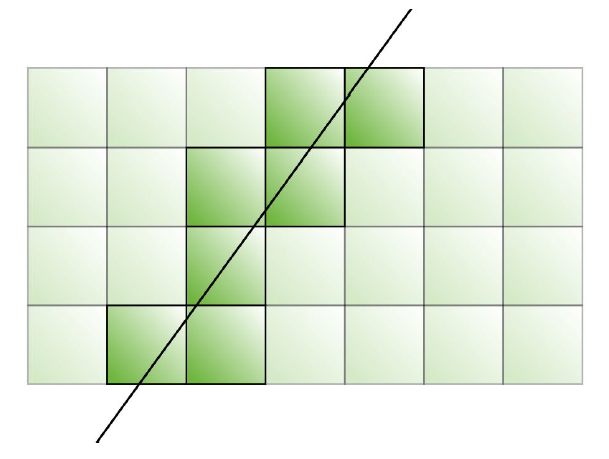
\includegraphics[width=7cm]{pics/linetemplate.png}
\end{center}
}

\end{document}